% !TeX spellcheck = en_GB
\documentclass[letterpaper,twoside,12pt]{memoir}

\title{Harnessing Neural Dynamics\\as a Computational Resource}%:\\Building Blocks for Computational Neuroscience and Artificial Agents}
\author{Andreas Stöckel}

% Setup microtype for pdfLaTex
\usepackage[final,tracking=true,expansion=true]{microtype}

\usepackage[sb]{libertine} % or \usepackage[sb]{libertinus}
\usepackage[T1]{fontenc}
\usepackage{textcomp}
\usepackage[scaled=0.81]{beramono}
\usepackage[lcgreekalpha]{libertinust1math} % slanted integrals, by default
\usepackage{amsthm} % libertinust1math loads amsmath
\usepackage[scr=boondoxo,bb=boondox]{mathalfa} %Omit bb=boondox for default libertinus bb
\usepackage[utf8]{inputenc}

\captionnamefont{\sffamily\small\bfseries}
\captionstyle{\sffamily\small}

\setlength{\parskip}{0.5em}

% Page layout
\setlrmarginsandblock{2.83cm}{2.83cm}{*}
\setheaderspaces{*}{0.75cm}{*}
\setheadfoot{\baselineskip}{1.25cm}
%\setulmarginsandblock{4.4cm}{4.5cm}{*}
\setulmarginsandblock{3.4cm}{3.5cm}{*}
\setmarginnotes{0.5cm}{2cm}{0em}
\checkandfixthelayout

%\setsubsecheadstyle{\itshape\raggedright}
\setsubsecheadstyle{\itshape\large\raggedright}
\setsecnumdepth{subsection}
\settocdepth{subsection}

\newcommand{\parahead}[1]{\itshape{{#1}.}\hspace{0.5em}}
\setparaindent{0em}
\setbeforeparaskip{\parskip}
\setafterparaskip{0em}
\setparaheadstyle{\parahead}

\newcommand{\subsubhead}[1]{\bfseries{{#1}.}\hspace{0.5em}}
\setsubsubsecindent{0em}
\setbeforesubsubsecskip{1em}
\setaftersubsubsecskip{0em}
\setsubsubsecheadstyle{\subsubhead}

% Header and footer setup
\nouppercaseheads
\makeatletter
\makepagestyle{headings}
\makepsmarks{headings}{%
	\createmark{chapter}{left}{shownumber}{\@chapapp\ }{. \ }
	\createmark{section}{right}{shownumber}{}{. \ }
	\createplainmark{toc}{both}{\contentsname}
	\createplainmark{lof}{both}{\listfigurename}
	\createplainmark{lot}{both}{\listtablename}
	\createplainmark{bib}{both}{\bibname}
	\createplainmark{index}{both}{\indexname}
	\createplainmark{glossary}{both}{\glossaryname}
}
\makeatother
\makeevenhead{headings}{\small\sffamily\leftmark}{}{}
\makeoddhead{headings}{}{}{\small\sffamily\rightmark}
\makeevenfoot{headings}{}{\small\sffamily\thepage}{}
\makeoddfoot{headings}{}{\small\sffamily\thepage}{}
\pagestyle{headings}

\copypagestyle{chapter}{plain}
\makeevenfoot{chapter}{}{\small\sffamily\thepage}{}
\makeoddfoot{chapter}{}{\small\sffamily\thepage}{}

\renewcommand{\contentsname}{Table of Contents}

% See https://stackoverflow.com/a/46767059
\makeatletter
\newenvironment{OpeningQuote}{\begingroup\small\raggedleft\begin{minipage}{0.9\textwidth}}{\end{minipage}\\[2em]\endgroup\def\if@endpe{\@doendpe\let\par\@@par\iffalse}}
\makeatother
\newcommand{\OpeningQuoteSource}[2]{\par\vspace{0.5em}\raggedleft--- \textsc{#1}\\\textit{#2}}

\newenvironment{PriorPublication}{
\begin{figure}[b!]
\rule{\textwidth}{2pt}\\[0.25em]
\small%
\sffamily%
\textbf{Material in this chapter from prior publications}\\[0.25cm]
}{
\end{figure}
}

\newenvironment{Contributions}{
\begin{figure}[b!]
\small%
\sffamily%
\textbf{Contributions in this chapter}\\[0.25cm]
}{
\end{figure}
}
\usepackage{amsmath}
\usepackage{amsthm}
\usepackage{amssymb}
\usepackage{graphicx}
\usepackage{csquotes}
\usepackage{mathrsfs} % mathscr
\usepackage{mathtools}
\usepackage{booktabs}
\usepackage{xspace}
\usepackage{longtable}
\usepackage{multirow}
\usepackage{rotating}

\usepackage{marvosym} % Lightning symbol

% Restateable theorems
\usepackage{thmtools}
\usepackage{thm-restate}


%\usepackage{imakeidx}

\usepackage[toc,acronym]{glossaries} % Glossary.
%\usepackage{glossary-mcols}

\usepackage[labelfont={small,bf,sf},textfont={small,sf}]{caption}
\usepackage{subcaption}

\usepackage[a-1b]{pdfx}

% Setup Bibtex

\usepackage[
	style=authoryear,
	uniquename=false,
	mincitenames=1,
	maxcitenames=1,
	citetracker=true,
	natbib=true,
	sorting=nyt,
	hyperref=true,
	backref=false]{biblatex}
\setlength{\bibnamesep}{0.5em}


% See https://tex.stackexchange.com/a/478787
\makeatletter
\AtEveryCitekey{%
  \ifciteseen
    {}
    {\defcounter{maxnames}{3}}%
}
\makeatother

\usepackage{siunitx}

%\DefineBibliographyStrings{english}{%
%  backrefpage = {cited on page~},
%  backrefpages = {cited on pages~},
%}

\DeclareFieldFormat{citehyperref}{%
  \DeclareFieldAlias{bibhyperref}{noformat}% Avoid nested links
  \bibhyperref{#1}}

\DeclareFieldFormat{textcitehyperref}{%
  \DeclareFieldAlias{bibhyperref}{noformat}% Avoid nested links
  \bibhyperref{%
    #1%
    \ifbool{cbx:parens}
      {\bibcloseparen\global\boolfalse{cbx:parens}}
      {}}}

%\savebibmacro{cite}
%\savebibmacro{textcite}
%
%\renewbibmacro*{cite}{%
%  \printtext[citehyperref]{%
%    \restorebibmacro{cite}%
%    \usebibmacro{cite}}}
%
%\renewbibmacro*{textcite}{%
%  \ifboolexpr{
%    ( not test {\iffieldundef{prenote}} and
%      test {\ifnumequal{\value{citecount}}{1}} )
%    or
%    ( not test {\iffieldundef{postnote}} and
%      test {\ifnumequal{\value{citecount}}{\value{citetotal}}} )
%  }
%    {\DeclareFieldAlias{textcitehyperref}{noformat}}
%    {}%
%  \printtext[textcitehyperref]{%
%    \restorebibmacro{textcite}%
%    \usebibmacro{textcite}}}
%

\definecolor{linkBlue}{HTML}{003399}
\definecolor{linkGreen}{HTML}{2E8B57} % SeaGreen

\usepackage{hyperref} % with basic options
\hypersetup{
    pdfborder={0 0 0},
    plainpages=false,
    unicode=true,
    colorlinks=false,
%    colorlinks=true,
%    allcolors=linkBlue,
%    citecolor=linkGreen
}
\usepackage{cleveref}
\renewcommand\thesubfigure{\Alph{subfigure}}

\theoremstyle{theorem}
\declaretheorem{theorem}
\declaretheorem[name=Claim]{claim}
\declaretheorem[name=Lemma]{lemma}

\theoremstyle{definition}
\newtheorem{definition}{Definition}[chapter]
\DeclareMathOperator{\vol}{vol}

\renewcommand{\vec}[1]{\mathbf{#1}}
\newcommand{\mat}[1]{\mathbf{#1}}
\newcommand{\tmp}[1]{\mathfrak{#1}}
\renewcommand{\phi}{\varphi}
\renewcommand{\epsilon}{\varepsilon}
%\newcommand{\oh}{\mathcal{o}}
\newcommand{\oh}{o}

\DeclareMathOperator{\diag}{\mathrm{diag}}
\DeclareMathOperator{\adj}{\mathrm{adj}}
\DeclareMathOperator{\sign}{\mathrm{sgn}}
\DeclareMathOperator{\correspondsTo}{\overset{\wedge}{=}}
\DeclareMathOperator{\supposedEq}{\overset{!}{=}}
\DeclareMathOperator{\lstsqEq}{{=\kern-0.8em{\raisebox{0.35em}\sim\hspace{0.1em}}}}


%% DRAFT 
%\usepackage{showframe}
\usepackage[normalem]{ulem}
\usepackage{lipsum}
\usepackage[textsize=small]{todonotes}

\newglossarystyle{symbols}{%
  \setglossarystyle{long}%
  \renewenvironment{theglossary}%
     {\renewcommand{\arraystretch}{1.25}%
      \begin{longtable}[l]{@{}p{\dimexpr 1cm-\tabcolsep}p{\dimexpr \textwidth-1.25cm}}}
     {\end{longtable}}%
 }
\newglossarystyle{acronyms}{%
  \setglossarystyle{long}%
  \renewenvironment{theglossary}%
     {\renewcommand{\arraystretch}{1.25}%
      \begin{longtable}[l]{@{}p{\dimexpr 2cm-\tabcolsep}p{\dimexpr \textwidth-2.25cm}}}
     {\end{longtable}}%
 }


\addbibresource{bibliography.bib}

\makeindex

% Starts creation of a glossary.
\makeglossaries
% !TeX spellcheck = en_GB

\newcommand*{\Reals}{\gls{Reals}\xspace}
\newglossaryentry{Reals}{
	name=\ensuremath{\mathbb{R}},
	type=symbols,
	sort=Reals,
	description={The real number-line, i.e., all values of a scalar magnitude},
}

\newcommand*{\Ball}{\gls{Ball}\xspace}
\newglossaryentry{Ball}{
	name=\ensuremath{\mathbb{B}},
	type=symbols,
	sort=Ball,
	description={A hyperball, the set of all $d$ dimensional vectors within radius $r$ of the coordinate origin, in other words
	$r \mathbb{B}^d = \{ \vec x \in \mathbb{R}^d \mid \, \|x\|_2 \leq r \}$,
	where the notation $r \mathbb{B}^d$ denotes the radius $r$ and dimensionality $d$ of the hyperball
	},
}


\newcommand*{\Normal}{\gls{Normal}\xspace}
\newglossaryentry{Normal}{
	name=\ensuremath{\mathcal{N}},
	type=symbols,
	sort=Normal,
	description={The normal distribution. The notation $\nu \sim \mathcal{N}(\mu, \sigma)$ indicates that $\nu$ is a normal-distributed random variable with mean $\mu$ and standard deviation $\sigma$},
}

\newcommand*{\Dec}{\gls{Dec}\xspace}
\newglossaryentry{Dec}{
	name=\ensuremath{\mat{D}},
	type=symbols,
	sort=Dec,
	description={A decoding matrix of shape $\mathbb{R}^{d \times \Npop}$. Decoding matrices are used within the Neural Engineering Framework to either reconstruct the value represented by a population of neurons (the identity decoder) or to decode a specific function. In the latter case, we sometimes write $\mat{D}^f$ to denote the function that is being decoded.},
}

\newcommand*{\Npop}{\gls{Npop}\xspace}
\newglossaryentry{Npop}{
	name=\ensuremath{n},
	type=symbols,
	sort=npop,
	description={Number of neurons in a neuron population.
	This determines the dimensionality of the associated activity vector $\vec a$},
}

\newcommand*{\Nsmpls}{\gls{Nsmpls}\xspace}
\newglossaryentry{Nsmpls}{
	name=\ensuremath{N},
	type=symbols,
	sort=Nsmpls,
	description={This symbol is typically used to indicate the number of samples in an optimization problem},
}

\newcommand*{\Ndim}{\gls{Ndim}\xspace}
\newglossaryentry{Ndim}{
	name=\ensuremath{d},
	type=symbols,
	sort=Ndim,
	description={Number of dimensions represented by a neuron population},
}

\newcommand*{\Xrepr}{\gls{Xrepr}\xspace}
\newglossaryentry{Xrepr}{
	name=\ensuremath{\mathbb{X}},
	type=symbols,
	sort=Xrepre,
	description={Set of possible values represented by a neuron population. We assume that this is a compact set with finite volume, i.e., $\vol(\mathbb{X})$},
}


\newcommand*{\vRest}{\gls{vRest}\xspace}
\newglossaryentry{vRest}{
	name=\ensuremath{v_\mathrm{rest}},
	type=symbols,
	sort=vrest,
	description={Resting potential of a neuron.
	This is the membrane potential that can be measured in a neuron when no input is applied.
	In vertebrates the resting potential is typically close to \SI{-65}{\milli\volt}.
	The resting potential is generally equal to the \enquote{leak potential} \EL, though different in semantics}
	% TODO check potentials
}

\newcommand*{\vReset}{\gls{vReset}\xspace}
\newglossaryentry{vReset}{
	name=\ensuremath{v_\mathrm{reset}},
	type=symbols,
	sort=vreset,
	description={Reset potential. TODO}
	% TODO check potentials
}


\newcommand*{\vTh}{\gls{vTh}\xspace}
\newglossaryentry{vTh}{
	name=\ensuremath{v_\mathrm{th}},
	type=symbols,
	sort=vth,
	description={Threshold potential. TODO}
	% TODO check potentials
}


\newcommand*{\CMem}{\gls{CMem}\xspace}
\newglossaryentry{CMem}{
	name=\ensuremath{C_\mathrm{m}},
	type=symbols,
	sort=Cm,
	description={Membrane capacitance. TODO}
}

\newcommand*{\EL}{\gls{EL}\xspace}
\newglossaryentry{EL}{
	name=\ensuremath{E_\mathrm{L}},
	type=symbols,
	sort=EL,
	description={Leak potential. In contrast to the resting potential \vRest, which is an empirical measurement, the leak potential $E_\mathrm{L}$ is the reversal potential of a so-called \enquote{leak-channel}.
	The leak-channel merely a modelling convenience that summarises the state of multiple ion channels of the neuron at rest}
	% TODO check potentials
}

\newcommand*{\gL}{\gls{gL}\xspace}
\newglossaryentry{gL}{
	name=\ensuremath{g_\mathrm{L}},
	type=symbols,
	sort=gL,
	description={Leak conductance. TODO}
}


\newcommand*{\gE}{\gls{gE}\xspace}
\newglossaryentry{gE}{
	name=\ensuremath{g_\mathrm{E}},
	type=symbols,
	sort=gE,
	description={Excitatory conductance. TODO}
}

\newcommand*{\gI}{\gls{gI}\xspace}
\newglossaryentry{gI}{
	name=\ensuremath{g_\mathrm{I}},
	type=symbols,
	sort=gI,
	description={Inhibitory conductance. TODO}
}



\begin{document}

	%\frontmatter
	%% !TeX spellcheck = en_GB
\thispagestyle{empty}
\begin{center}
	\sffamily
	\vfill
	\Huge
	\thetitle
	
	\vfill
	
	\normalsize
	by \\
	
	\vfill
	
	\Large
	\theauthor \\
	
	\vfill
	\vfill
	\vfill
	
	\normalsize
	A thesis \\
	presented to the University of Waterloo \\ 
	in fulfillment of the \\
	thesis requirement for the degree of \\
	Doctor of Philosophy \\
	in \\
	Computer Science \\
	
	\vfill
	\vfill

	Waterloo, Ontario, Canada, 2021 \\
	
	\vfill
	
	\copyright\ \theauthor~2021 \\
\end{center}
\clearpage
	%% !TeX spellcheck = en_GB
\begin{center}\textbf{Examining Committee Membership}\end{center}

  \bigskip

  \noindent
The following served on the Examining Committee for this thesis. The decision of the Examining Committee is by majority vote.
  \bigskip
  
  \noindent
\begin{tabbing}
Internal-External Member \quad \=  \kill % using longest text to define tab length
External Examiner \>  Wulfram Gerstner \\ 
\> Professor, \\
\> School of Life Sciences and\\
\> School of Computer and Communication Sciences, \\
\> École Polytechnique Fédérale de Lausanne\\[0.75cm]
%%%%
Supervisor \> Chris Eliasmith \\
\> Professor, \\
\> Department of Philosophy and \\
\> Department of Systems Design Engineering, \\
\> University of Waterloo \\[0.75cm]
%%%%
Internal Member \> Robin Cohen \\
\> Professor, \\
\> Department of Computer Science, \\
\> University of Waterloo \\[0.5cm]
%%%%%
Internal Member \> Jeff Orchard \\
\> Professor, \\
\> Department of Computer Science, \\
\> University of Waterloo \\[0.5cm]
%%%%%
Internal-External Member \> Sue Ann Campbell \\
\> Professor, \\
\> Department of Applied Mathematics, \\
\> University of Waterloo
\end{tabbing}

\clearpage
	%% !TeX spellcheck = en_GB
\begin{center}\textbf{Author's Declaration}\end{center}

\noindent
This thesis consists of material all of which I authored or co-authored: see Statement of Contributions included in the thesis. This is a true copy of the thesis, including any required final revisions, as accepted by my examiners.

\bigskip

\noindent
I understand that my thesis may be made electronically available to the public.

\clearpage
	%% !TeX spellcheck = en_GB
\phantomsection
\addcontentsline{toc}{chapter}{Statement of Contributions}
\begin{center}\textbf{Statement of Contributions}\end{center}

Andreas Stöckel is the sole author of Chapters 1, 4, and 6.
These chapters were either not written for publication or are based on self-published technical reports.
The remaining chapters are, in heavily edited and extended form, based on the following published works:

\begin{enumerate}
	\item[{[1]}] \fullcite{stoeckel2021}
	\item[{[2]}] \fullcite{stockel2021connecting}
\end{enumerate}

\noindent Use of these publications in this thesis is with permission of the publishers.
All figures in this thesis, with the sole exception of \Cref{fig:izhikevich_whichmod_figure1}, were created by the author.
Annotations such as \enquote{inspired by} or \enquote{adapted from} merely indicate the source of the presented information.

\subsubsection{Contributions to the individual publications}

\begin{enumerate}
	\item[{[1]}] This research was conducted by Andreas Stöckel.
	Chris Eliasmith supervised this work and helped designing the experiments.
	Andreas Stöckel wrote all the underlying code, conducted the experiments, created the figures, and wrote the manuscript.
	Chris Eliasmith edited the manuscript.
	\item[{[2]}] This research was conducted by Andreas Stöckel and Terrence C.~Stewart.
	Andreas Stöckel was responsible for conducting the experiments, contributing the underlying theoretical work, writing, creating all figures, and conducting the literature review.
	Terrence C.~Stewart helped with designing the final network, exploring the parameter space, and writing the paper.
	Chris Eliasmith supervised this work, provided helpful feedback, and edited the manuscript.
\end{enumerate}

\subsubsection{Use of these publications in this thesis}

\begin{description}
	\item[\normalfont\emph{Chapter~2:}] Small parts of this chapter are based on [1], in particular the description of the Neural Engineering Framework in Sections~2.3.3-2.3.5.
	\item[\normalfont\emph{Chapter~3:}] The introduction of Chapter~3, and Sections 3.2-3.4, 3.6 are in part based on [1].
	The experiments in Section 3.3 and 3.4 and the corresponding figures are, with minor changes, as previous published.
	\item[\normalfont\emph{Chapter~4:}] This chapter is in large parts based on [2].
\end{description}

\clearpage

	%% !TeX spellcheck = en_GB
\begin{abstract}
\end{abstract}
\clearpage
	%% !TeX spellcheck = en_GB
\begin{center}\textbf{Acknowledgements}\end{center}

Foremost, I thank Loblaws for keeping me alive by selling food at reasonable prices.
I mean, if the president chooses it, it must be good!
Furthermore, I would like to thank the friendly Canadian border agent who did not deport me after I said that hockey sucks.
Lastly, I thank IKEA for furnishing my home; what would life be without Billy the bookshelf?

\vfill

\todo[inline]{Write acknowledgements}


\clearpage

	%% !TeX spellcheck = en_GB
{
\noindent
\raggedleft
\emph{To Margaret, the spider.\\You vanished prematurely from our lives;\\one day, you were hunting in your usual spot\\behind the kitchen cutting boards;\\the other day, you were gone.\\[0.5em]May we never forget you.}\\
\vfill
\raggedright
\includegraphics[width=0.4\textwidth]{media/margaret.jpg}
\vfill
\todo[inline]{Write dedication}
\clearpage
}

	%\tableofcontents
	%\clearpage
	%\listoffigures
	%\clearpage
	%\listoftables

	\mainmatter

	%\setcounter{chapter}{0}
	%\include{chapters/chapter_introduction}

	%\setcounter{chapter}{1}
	%% !TeX spellcheck = en_GB
\chapter{Modelling Neurobiological Systems}
\label{chp:modelling_neurobiological_systems}

\chapterprecishere{First, it is an overstatement to describe what I am attempting here as an \enquote{approach toward the understanding}; it is merely a somewhat systematized set of speculations as to how such an approach ought to be made. That is, I am trying to guess which of the---mathematically guided---lines of attack seem, from the hazy distance in which we see most of them, a priori promising, and which ones have the opposite appearance.\par\raggedleft--- \textup{John von Neumann}, The Computer and the Brain (1958)}

%\begin{Contributions}
%We primarily review fundamental neurobiology, as well as prior work in the form of the Neural Engineering Framework.
%The author's main contribution lies in the presentation of the material.
%\end{Contributions}

\begin{PriorPublication}
Parts of this chapter, particularly \Cref{sec:nef}, are based on \citet{stoeckel2021}.
Some figures in this chapter were adapted from material previously prepared for the University of Waterloo course SYDE 556/720, \enquote{Simulating Neurobiological Systems} taught by the author in winter 2020.
\end{PriorPublication}

The desire to understand cognition is by no means a new one---wondering about one's own thought processes has surely been part of the human condition since prehistoric times.
Today, we know that nerve cells in the brain are the primary functional and structural units that give rise to biological cognition.
This is referred to as the \emph{neuron doctrine}\index{neuron doctrine}, a view that garnered support through observations made by Santiago Ramón y Cajal\index{Ramón y Cajal, Santiago} and Charles Scott Sherrington\index{Sherrington, Charles Scott} at the turn of the nineteenth century \citep[Chapter~2]{yuste2015neuron,bear2016neuroscience}.
%Highly debated at the time, an alternative view was that the nervous system is a single entity, comparable to the then well understood network of blood vessels \citep[Chapter~2]{bear2016neuroscience}.

Although the nature of neurons as independent units is undisputed, the neuron doctrine continues to be scrutinised.
There is an argument to be made that neural circuits are better described from the perspective of neural ensembles\index{neural ensemble} instead of individual neurons \citep{yuste2015neuron,churchland1992computational}---an idea that we revisit in the context of population codes.
Furthermore, it is still a matter of debate in how far structures such as Glial cells\index{glial cell}, must be taken into account to accurately model brain function \citep[e.g.,][]{verkhratsky2000ion}.
%Indeed, some scientists take rather extreme stances regarding the influence of Glial cells on high-level cognition \citep[e.g.,][]{agid2021glial}.

%Some fundamental questions, such as what the best abstractions for describing brain function are, or what kind of structures should be included in models, garner little consensus among scientists.

\begin{figure}
	\centering
	\includegraphics{media/chapter_modelling_neurobiological_systems/levels.pdf}
	\caption[Illustration of temporal and spatial scales in neuroscience]{Illustration of temporal and spatial scales in neuroscience. Placement of individual concepts is a deliberately coarse estimate and, in some cases, open to debate. Spatial scale and levels of organisation adapted from \citet[Figure~1.4, p.~11]{churchland1992computational}.}
	\label{fig:spatial_and_temporal_scales}
	\vspace*{-0.5em}
\end{figure}

%While some of this dissent is simply due to researchers focusing on different aspects of the brain,
The fact that,  after more than a century of research, such fundamental debates still persist, illustrates that neuroscience (and by extension the other cognitive sciences) are still in their early days.
This is not due to a lack of talent or dedication;
rather, the gaps in our knowledge are a testament to the intrinsic difficulty of understanding complex systems such as the brain.

In some regard, neuroscience may be compared to physics.
Both study and predict the behaviour of natural systems, and both study phenomena that span vast spatial and temporal scales
%For example, in neurobiology, understanding neural mechanisms requires an analysis of molecular processes on the scale of nanometres and microseconds, while the behaviour of an organism can span metres and decades
(cf.~\Cref{fig:spatial_and_temporal_scales}).
Unlike physics, neuroscience is concerned with the behaviour of living objects consisting of billions of complex elements.%
\footnote{The human brain has $67$-$86\times10^{9}$ neurons and $\sim$$85\times10^9$ glial cells \citep{vonbartheld2016search}. Each neuron in cerebral cortex possesses $10^3$-$10^4$ synapses \citep[Chapter~6]{braitenberg2013anatomy}.}
The evolved nature of brains in particular makes it challenging to disentangle structures merely responsible for metabolic function, from those orchestrating behaviour.
Therefore, as demanded by many in the field \citep[e.g.,][]{marr1982vision,churchland1992computational,eliasmith2003neural}, neuroscience should be guided by predictive computational modelling and theory.%, with the goal to systematically connect mechanisms to behaviour, and to abstract unnecessary detail.

Here, the term \enquote{theory}, refers to overarching concepts applicable to different models \citep[e.g.,][]{stevens2000models}.
Continuing our physics analogy, successful physical theories such as Newtonian or Lagrangian mechanics, describe phenomena at different scales---from falling apples to solar systems orbiting their galactic centre.
Translating this to neuroscience, we would like our theories to connect low-level mechanisms (e.g., neurons, synapses, action potentials) to high-level behaviour (e.g.,~motor control, decision making, language).
As of now, there is no widely accepted theory that accomplishes this \citep{eliasmith2013how}.

All this is not to say that neuroscience has stagnated over the past decades.
To the contrary.
New recording methods---such as fMRI (functional magnetic resonance imaging), high-density multi-electrode arrays, calcium imaging, and optogenetics---have widened our perspective on brain function \citep{sejnowski2014putting}. Researchers have mapped out individual brain circuits \citep[e.g.,][]{shepherd2012handbook}, can describe neurons at a molecular level \citep[e.g.,][]{sobolevsky2009xray}, and determined the roles specific brain regions play in cognition \citep[e.g.,][]{kanwisher2006fusiform}.

Paradoxically, recent progress in neuroscience has made finding theories that bridge multiple levels of analysis \emph{more}, and not less important.
The central challenge is that each dataset on its own is fairly limited, mostly because different recording techniques possess dissimilar temporal and spatial characteristics \citep{sejnowski2014putting}.
The data we have access to is not detailed enough to directly inform large-scale models, and our theories are not sophisticated enough to combine heterogneous datasets. As already pointed out by \citet{churchland1992computational}, neuroscience has been, and still is, \enquote{data poor \emph{and} theory poor}.
A major difficulty in modelling brain function hence lies in building models that can be constrained by, and that make predictions compatible with, the different scales at which current recording techniques operate (\cite{eliasmith2003neural}, Chapter~1; \cite{eliasmith2013how}).

There are a few attempts at developing such theories, or, less ostentatiously, \emph{modelling frameworks}, that facilitate describing the nervous systems at different scales.
Examples include the Neural Engineering Framework (NEF)~\citep{eliasmith2003neural}, Efficient, Balanced Spiking Networks (EBN)~\citep{boerlin2011spikebased,boerlin2013predictive}, and FORCE~\citep{sussillo2009generating,nicola2017supervised}.
Generally speaking, these approaches describe how to translate dynamical systems---corresponding to some hypothesized behavioral model---into an idealized spiking neural network that adheres to desired neurophysiological constraints, such as neural tuning, firing rate distributions, and population-level connectivity ~\citep{komer2016unified,nicola2017supervised}.
The resulting networks can then be analysed using the same techniques as biological systems, bridging gap between empirical data and theory.

The goal of the first part of this thesis is to extend the Neural Engineering Framework to better take mechanistic constraints often found in the neuroscience literature into account.
To this end, we first review of fundamental neuroscientific concept, and continue with a description of the NEF, as well as a list of biological constraints currently not well-captured by the NEF.
We then, in subsequent chapters, propose extensions to the NEF that alleviate these issues.
Subsequently, we use some of these techniques to construct a model of eyeblink conditioning in the cerebellum.
In the second part of this thesis, we then apply the concepts we discussed in the context of modelling neurobiological systems to machine learning.

\clearpage

\section{Morphology and Physiology of Individual Neurons}
\label{sec:neurophysiology}

\begin{figure}
	\centering
	{\phantomsubcaption\label{fig:neuron_sketches_motor}}%
	{\phantomsubcaption\label{fig:neuron_sketches_pyramidal}}%
	{\phantomsubcaption\label{fig:neuron_sketches_purkinje}}%
	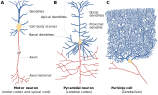
\includegraphics{media/chapter_modelling_neurobiological_systems/neuron_sketches.pdf}
	\caption[Drawings of neurons in different brain regions]{Drawings of neurons in different brain regions.
	Although key structural elements can be identified across neurons, they can have wildly different morphologies.
	Redrawn from Ramón y Cajal.
	Overall presentation from \citet{kandel2012principles}, Figure~2-3D, p.~25.
	\textbf{(A)} Schematic drawing of a motor neuron (\cite{ramonycajal1894nouvelles}, Figure 6, p.~25).
	\textbf{(B)} Human cortical pyramidal neuron (\cite{howell1916textbook}, Figure~84, p.~187).
	\textbf{(C)} Human purkinje cell in the cerebellum (\cite{ramonycajal1909histologie}, Figure~9, p.~61).
	\label{fig:neuron_sketches}
	}
\end{figure}

Neurons come in various sizes, shapes, and degrees of interconnectedness.
Ramón y Cajal's\index{Ramón y Cajal, Santiago} drawings (schematically redrawn in \Cref{fig:neuron_sketches}) offer a glimpse of the morphological diversity found in the nervous system.
Some neurons possess only few branches (also \emph{projections}\index{neuron!projection}) and have a comparably simple structure, whereas others, such as Cerebellar Purkinje cells, feature sprawling dendritic trees more deserving of the name \enquote{dendritic forest}.

It should come as no surprise that the following review of neural morphology and physiology cannot do justice to the sheer complexity observed in nature.
Our goal is to instead focus on structural and functional elements commonly observed across all neurons.
As a side-effect, the resulting characterisation of the nervous system lends itself well to computational models.
%While the simplifications we make come at the risk of ignoring details that could turn out to be essential for modelling brain function, some simplification
%Yet, as discussed above, we would like to develop theories that bridge as many levels of scale as possible.
%The aspects of biology that we incorporate into our models are known to play a major role in overall brain function.
We open with a high-level overview of neural function and structure, and then focus on aspects of neural electrophysiology that will be relevant in later sections, including the generation of the membrane potential, action potentials, and synaptic transmission.
Readers interested in a more thorough introduction to neuroscience are encouraged to consult introductory neuroscience textbooks such as \citet{bear2016neuroscience}, \citet{purves2017neuroscience}, or \citet{kandel2012principles}.

\subsection{Functional and Structural Overview}
\label{sec:neurons_overview}

\begin{figure}
	\centering
	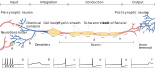
\includegraphics{media/chapter_modelling_neurobiological_systems/neuron_signals_overview.pdf}
	\caption[Schematic overview of neural function]{Schematic overview of neural function. Inset diagrams illustrate the membrane potential over time at the indicated locations (data from simulations of an instructional compartmental Hodgkin-Huxley type model neuron). Arrows indicate the predominant flow of information. \emph{Input:} Neurons receive signals from pre-neurons through synapses. For chemical synapses, action potentials (\enquote{spikes}) arriving at the pre-synapse (\emph{a}) cause a release of neurotransmitter that induces a post-synaptic potential (PSP) in the neuron (\emph{b}). \emph{Integration:} PSPs from multiple pre-neurons interact in the dendrites. Under certain conditions the neuron produces its own action potential (\emph{c}). \emph{Conduction:} The action potential travels along the axon (\emph{d}-\emph{e}). \emph{Output:} The neuron induces a PSP in its post-synaptic neuron (\emph{f}).
	}
	\label{fig:neuron_signal_overview}
\end{figure}

From the perspective of computer science---and as suggested by the neuron doctrine---neurons are fundamental units of computation in biological systems.
Specifically, neurons employ weak bioelectric signals, variations in their membrane potential, to compute.
As depicted in the lower portion of \Cref{fig:neuron_signal_overview}, these variations can either be gradual, as is the case when the neuron is in its \emph{subthreshold} regime\index{membrane potential!subthreshold}, or manifest themselves as rapid swings between the highest and lowest voltages that can be produced by a neuron; in this case the neuron is in its \emph{superthreshold} regime.
These rapid voltage changes are called \emph{action potentials}\index{action potential}, or, more colloquially, \enquote{\emph{spikes}}, harking back to their prominent appearance on oscillograms.
% TODO: Index: spike -> action potential

Typically, gradual subthreshold potentials are not directly accessible from other parts of the network;
this analogue code is solely part of a neuron's internal state.
Hence, from the perspective of other neurons in the network, a neuron is either \enquote{silent} or \enquote{spiking}.
This binary nature of neurons fascinated early computer scientists such as \citet{vonneumann1958computer}\index{Von Neumann,John} and led to the development of the first artificial neural networks by \citet{mcculloch1943logical}.

Neuroscientists typically divide neural information processing into four stages: input, integration, conduction, and output \citep[Chapter 2]{kandel2012principles}.
These stages roughly correspond to different features of neural structure, as depicted in \Cref{fig:neuron_signal_overview}.

The \emph{input region} corresponds to the so-called dendrites, and the synapses embedded therein.%
\footnote{
The difference between input and output regions of a neuron is not always clear-cut.
Invertebrate unipolar cells only possess a single branch that protrudes from the cell body.
This branch is referred to as \enquote{axon} although it carries both input and output \citep[Chapter~2]{kandel2012principles}.}
Dendrites are tree-like structures protruding out of the cell body, and are typically less than two millimetres long \citep[Chapter~1]{bear2016neuroscience}.
They are usually classified according to their location relative to the cell body.
For example, in pyramidal cells (cf.~\Cref{fig:neuron_sketches_pyramidal}) dendrites directly connected to the soma are called \emph{basal}\index{dendrite!basal}; dendrites indirectly connected to the soma through longer projections are called \emph{apical}\index{dendrite!apical}.
Apical dendrites are sometimes additionally divided---using standard anatomical terminology---into parts referred to as \emph{proxmial} or \emph{distal}; that is, they are either closer or father away from the soma \citep[e.g.,][Figure~5]{seamans1997contributions}.

Synapses form the coupling sites between neurons and---in the case of chemical synapses, and as discussed in more detail below---establish a unidirectional flow of information.
This ensures that pre-synaptic neurons only influence the state of the post-synaptic neuron, but not vice-versa \citep[Chapter~8]{kandel2012principles}.
Some neurons in the periphery of the nervous system act as sensors; they transduce modalities such as temperature, pressure or light and do not rely on synaptic inputs \citep[Chapter~22]{kandel2012principles}.

The neuron's \emph{integration region} is formed by the cell body and, to some degree, the dendritic tree itself.
Signals from several pre-neurons interact here.
This interaction may elicit the generation of an output signal.
As we mentioned before, this output takes the form of an \emph{action potential}\index{action potential} in most vertebrate neurons \citep[Chapter~2]{kandel2012principles}.
Crucially, and in contrast to artificial neural networks, the integration process has a temporal component.
That is, the input \emph{history} is relevant for the generation of the output, and not just the momentary input.

The \emph{conductive region} corresponds to a neuron's axon\index{axon}.
The axon carries signals generated by the neuron to other parts of the nervous system.
Two features of the axon work in tandem to ensure signal integrity \citep[Chapter~7]{kandel2012principles}.
First, the axon is electrically well insulated, being tightly wrapped in Schwann's cells\index{Schwann's cell}, a type of glial cell\index{glial cell}.
Second, axons actively renew action potentials at Nodes of Ranvier\index{Node of Ranvier}, gaps between neighbouring glial cells.
Conduction is unidirectional in the sense that action potentials only travel away from the origin of excitation.
Notably, in larger animals such as humans, individual neurons conduct signals across micrometres (between neighbouring neurons), centimetres (connecting different parts of the brain), and metres (motor neurons in the spinal cord).%

Finally, the \emph{output region} corresponds to synapses embedded in the axon terminals.
These synapses connect to the input region of post-neurons, completing the cycle.
In the case of chemical synapses, the arrival of an action potential at the pre-synapse, the \enquote{synaptic bouton}\index{synaptic bouton}, causes the release of neurotransmitter molecules.
Receptors in the post-neuron transduce neurotransmitters into an input signal, a so-called post-synaptic potential.
In the periphery, axon terminals may be electrically coupled to muscle fibres, where the arrival of an action potential generates movement \citep[Chapter~8 \& 9]{kandel2012principles}.

\subsection{Ion channels and the membrane potential}
\label{sec:membrane_potential}

\begin{figure}
	\centering
	{\phantomsubcaption\label{fig:neuron_membrane_potential_membrane}}%
	{\phantomsubcaption\label{fig:neuron_membrane_potential_membrane_isolated}}%
	{\phantomsubcaption\label{fig:neuron_membrane_potential_membrane_channel}}%
	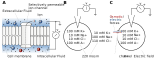
\includegraphics{media/chapter_modelling_neurobiological_systems/neuron_membrane_potential.pdf}
	\caption[Membrane potential as a result of selectively permeable ion channels]{
	Membrane potential as a result of selectively permeable ion channels.
	\textbf{(A)} The cell membrane separates the intra- and extracellular fluid. Charge carriers (e.g., ions) are in solution in the fluids. The membrane potential is the voltage \vMem across the membrane.
	Specific ions may pass through selectively permeable channels.
	\textbf{(B)} If the membrane was a perfect insulator, there would be no membrane potential. Molar concentration in $\mathrm{mM} = \si{\milli\mole\per\litre}$; values illustrative. $A^-$ corresponds to charged anionic molecules.
	The individual fluids are electrically neutral.
	\textbf{(C)} Adding a selectively permeable ion channel results in a membrane potential specific to the ion species at which electric and osmotic forces cancel out.
	Illustrations (B, C) adapted from \citet{reichert2000neurobiologie}, Figures 2.8 and 2.10.}
\end{figure}

As mentioned above, neurons process information by systematically varying their membrane potential\index{membrane potential}\index{potential!membrane} \vMem (more precisely, their \emph{transmembrane} potential).
The membrane potential is the electrical potential between the in- and outside of a cell.
The boundary between these regions is formed by the cell membrane, a double-layer of lipids.%
\footnote{To be clear, \emph{all} biological cells possess bioelectrical properties, including a membrane potential.
This was for example analysed in detail by Julius Bernstein\index{Bernstein, Julius} in the early 1900s \citep{bernstein1912elektrobiologie}. Membrane potentials are important for homeostasis and cell-to-cell communication \citep{moorhouse2016membrane}.
For example, electrical gradients between cells are crucial for laying out the body plan of organisms \citep{levin2014molecular}.
Neurons should be thought of as cells shaped by evolution to excel at bioelectrical signalling, but are not unique in their use of bioelectricity.}
By convention, if the \emph{inside} is more positively charged than the outside, we report a positive voltage (\Cref{fig:neuron_membrane_potential_membrane}).

Measuring the membrane potential when a neuron is at rest---that is, when the cell does not receive any input---reveals the so-called resting potential \vRest.
In mammals, \vRest ranges from \SIrange{-50}{-85}{\milli\volt} depending on the cell type \citep{moorhouse2016membrane}.

Upon closer investigation, the presence of a non-zero resting potential is rather surprising.
The in- and outside of the cell are filled with watery solutions: the intracellular fluid (\enquote{cytoplasm}\index{cytoplasm}) and the extracellular fluid.
Both fluids are electrically neutral.
That is, although the fluids contain ions and anionic charge carriers in solution, the overall positive and negative charges are balanced.
There should be no measurable electrical potential (\Cref{fig:neuron_membrane_potential_membrane_isolated}).


\subsubsection{Selectively permeable ion channels generate the membrane potential}
\begin{figure}
	\centering
	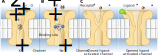
\includegraphics{media/chapter_modelling_neurobiological_systems/channel.pdf}%
	{\phantomsubcaption\label{fig:ion_channels_k}}%
	{\phantomsubcaption\label{fig:ion_channels_na}}%
	{\phantomsubcaption\label{fig:ion_channels_gate}}%
	\caption[Schematic illustration of ion channels  embedded into the cell membrane]{Schematic illustration of ion channels embedded in the cell membrane. Ion channels are pores that selectively let ions of a certain species pass. Selectivity is achieved by exploiting the radius and charge distributions of the ion and its watery hull. \textbf{(A)} Although the $\mathrm{K^+}$ ion is larger than the $\mathrm{Na^+}$ ion, its watery hull is more compact, and it can pass through narrower channels. \textbf{(B)}  $\mathrm{Na^+}$ selectivity is achieved by a negative binding site in the channel that stabilises the $\mathrm{K^+}$ ion and its hull to let it pass.  \textbf{(C)} Ion channels can change their conformation depending on external factors (e.g.~mechanical forces, chemicals, electrical potentials); here, a chemical ligand opens a channel. Inspired by \citet[Figure~5-1, p.~102 and Figure~5-6, p.~109]{kandel2012principles}; see ibid.~for more information.}
\end{figure}
The resting potential can be explained if we assume that the cell membrane is selectively permeable for some ions through so-called \emph{ion channels}\index{ion channel}.
The presence of ion channels has been postulated for a long time, though it is only thanks to relatively recent studies that we understand the molecular machinery that underpins selective permeability \citep[Chapter~5]{kandel2012principles}.

Ion channels are porous proteins embedded in the cell membrane.
They accomplish the impressive feat of acting as an \enquote{atomic sieve}.
This \enquote{sieve} only lets a single ion of a certain kind (in chemical parlance: \emph{ion species}\index{ion species}) pass at a time, as is illustrated in \Cref{fig:ion_channels_k,fig:ion_channels_na}.
Furthermore, as we will see both in the context of action potential generation and synaptic transmission, these proteins can change their shape, or \emph{conformation}, depending on various external circumstances, effectively opening or closing the channel (\Cref{fig:ion_channels_gate}).

Of course, the mere presence of selectively permeable channels does not explain the membrane potential.
For this, we have to consider that despite being electrically neutral, the intra- and extracellular fluids contain different concentrations of the individual charge carriers.
In particular, there are large concentration gradients for potassium ($\mathrm{K^+}$), sodium ($\mathrm{Na^+}$) and chloride ($\mathrm{Cl^-}$) ions.
For example, the concentration of potassium ions $\mathrm{K^+}$ is about \SI{140}{\milli\mol\per\litre} in the cytoplasm, compared to \SI{3}{\milli\mol\per\litre} in the extracellular fluid.
If the cell membrane was permeable for $\mathrm{K}^+$ ions, an osmotic force would act on the ions, driving them outside.

This ionic flow disturbs the charge balance of the intra- and extracellular fluids and results in a non-zero membrane potential.
In turn, this potential results in an electric force that counters the osmotic pressure.
In our $\mathrm{K}^+$ example, the intracellular fluid becomes negatively charged and the ensuing electric attraction reduces the net force acting on the $\mathrm{K}^+$ ions.
The system converges to an equilibrium point where the electric and osmotic forces cancel out (\Cref{fig:neuron_membrane_potential_membrane_channel}).
The membrane potential at this point is called the \emph{equilibrium}\index{equilibrium potential}\index{potential!equilibrium} or \emph{reversal potential}\index{reversal potential}\index{potential!reversal}, as the ionic flow direction reverses at this point.
For clarity, we use the term reversal potential when talking about the equilibrium potential for a membrane permeable for a \emph{single} ion.


\subsubsection{Single selectively permeable ion channel: Nernst equation}
For a single charge carrier $X$, the reversal potential $E_X$ can be computed using the Nernst equation\index{Nernst equation} \citep{nernst1888kinetik}:%
\footnote{The Nernst equation was published in 1888, before there were established theories about bioelectricity. Nernst studied the electrochemistry of electrolytes separated by membranes and this research was later incorporated into analyses of biological cell membranes by Ostwald and later Bernstein \citep[see][Chapter~5]{bernstein1912elektrobiologie}\index{Bernstein, Julius}.}
\newcommand{\Cout}[1]{\ensuremath{[\mathrm{#1}]_\mathrm{out}}}
\newcommand{\Cin}[1]{\ensuremath{[\mathrm{#1}]_\mathrm{in}}}
\begin{align}
	E_X &= -\frac{RT}{zF} \log \left( \frac{\Cin{X}}{\Cout{X}} \right) \,,
	\label{eqn:nernst}
\end{align}
where $R$ is the gas constant, $T$ is the temperature, $z$ is the charge number, or valence\index{valence}, of the particle (e.g., $z = 2$ for $\mathrm{Ca}^{2+}$ and $-1$ for $\mathrm{Cl}^-$) and $F$ is the Faraday constant. \Cout{X} and \Cin{X} are the concentrations (count per volume) of particles $X$ outside and inside the cell, respectively.
Note that the number of ions flowing through the cell membrane is rather minuscule compared to the total number of ions in solution; \Cout{X} and \Cin{X} essentially do not change over time.%
\footnote{The ion concentrations in the intra- and extracellular fluid are maintained by ion pumps in the cell membrane. These pumps are secondary for a cell's short-term bioelectrical properties, but are indispensible in the long run.}

\begin{table}
	\centering
	\caption[Ion concentrations and reversal potentials in the squid and mammals]{Ion concentrations and reversal potentials in the squid and mammals. Data from \citet[Table~12.1, p.~353]{mccormick2014membrane}. The squid data are based on \citet{hodgkin1949effect}, and reported similarly in \citet[Table~6-1, p.~128]{kandel2012principles}. Reversal potentials computed using \cref{eqn:nernst}.}
	\label{tbl:nernst}
	\small
	\sffamily
	\begin{tabular}{l l p{0.25cm} r r p{0.25cm} r r}
		\toprule
		&
		&
		& \multicolumn{2}{c}{\textbf{Concentrations}}
		&
		& \multicolumn{2}{c}{\textbf{Reversal potentials}} \\ %  \multicolumn{1}{c}{\textbf{Permeability ratios}}\\
		\cmidrule(lr){4-5}\cmidrule(lr){7-8}
		
		\multicolumn{2}{l}{\textbf{Ion species}}
		&
		& \emph{Intracellular}
		& \emph{Extracellular}
		&
		& $T = \SI{20}{\degreeCelsius}$
		& $T = \SI{36}{\degreeCelsius}$ \\ %& $P_\mathrm{K^+} : P_\mathrm{Na^+} : P_\mathrm{Cl^-}$ \\
		\midrule

		\multicolumn{2}{l}{\emph{Squid giant axon}}\\

		\raggedleft \quad Potassium
		& $\mathrm{K}^+$
		&
		& \SI{400}{\milli\mol\per\litre}
		& \SI{20}{\milli\mol\per\litre}
		&
		& \SI{-76}{\milli\volt}
		& \SI{-80}{\milli\volt} \\

		\raggedleft \quad Sodium
		& $\mathrm{Na}^+$
		&
		& \SI{50}{\milli\mol\per\litre}
		& \SI{440}{\milli\mol\per\litre}
		&
		& \SI{55}{\milli\volt}
		& \SI{58}{\milli\volt} \\

		\raggedleft \quad Chloride
		& $\mathrm{Cl}^-$
		&
		& \SI{40}{\milli\mol\per\litre}
		& \SI{560}{\milli\mol\per\litre}
		&
		& \SI{-67}{\milli\volt}
		& \SI{-70}{\milli\volt} \\[0.25cm]

		\multicolumn{2}{l}{\emph{Mammalian neuron}}\\

		\raggedleft \quad Potassium
		& $\mathrm{K}^+$
		&
		& \SI{140}{\milli\mol\per\litre}
		& \SI{3}{\milli\mol\per\litre}
		&
		& \SI{-97}{\milli\volt}
		& \SI{-102}{\milli\volt} \\

		\raggedleft \quad Sodium
		& $\mathrm{Na}^+$
		&
		& \SI{18}{\milli\mol\per\litre}
		& \SI{145}{\milli\mol\per\litre}
		&
		& \SI{53}{\milli\volt}
		& \SI{56}{\milli\volt} \\

		\raggedleft \quad Chloride
		& $\mathrm{Cl}^-$
		&
		& \SI{7}{\milli\mol\per\litre}
		& \SI{120}{\milli\mol\per\litre}
		&
		& \SI{-72}{\milli\volt}
		& \SI{-76}{\milli\volt} \\

		\bottomrule
	\end{tabular}
\end{table}

\subsubsection{Multiple selectively permeable ion channels: Goldman-Huxley-Katz equation}
\Cref{tbl:nernst} lists the ion concentrations of the squid giant axon, a model system common in the early days of neuroscience, as well as mammalian cells.
Although there are large differences in the ion concentrations, the reversal potentials (when computed using eq.~\ref{eqn:nernst}) are similar across species.
Still, we find that, in general, no individual reversal potential exactly matches the resting potential.
For example, in the squid, the resting potential is close to \SI{-62}{\milli\volt} at a temperature of \SI{20}{\degreeCelsius} (\cite{mccormick2014membrane}).
This potential is slightly more positive than $E_\mathrm{K^+}$ and $E_\mathrm{Cl^-}$, but much more negative than $E_\mathrm{Na^+}$.

This suggests that the cell membrane is permeable to several ion species at the same time, but at different \enquote{permeabilities}.
The membrane potential converges to a new equilibrium state $E$ somewhere between the original reversal potentials.
Mathematically, we summarise the relative permeability of the cell membrane for an ion species $X$ as a quantity $P_X$.
Instructively, $P_X$ can be interpreted as the total number of open ion channels for an ion species $X$.

We can compute the overall equilibrium potential using the Goldman-Huxley-Katz equation\index{Goldman-Huxley-Katz equation} \citep{goldman1943potential,hodgkin1949effect}.
For the three ion species listed above we have
\begin{align}
	E &= \frac{RT}{F} \log \left( \frac{
		P_\mathrm{K^+} \Cout{K^+} +
		P_\mathrm{Na^+} \Cout{Na^+} +
		P_\mathrm{Cl^-} \Cin{Cl^-}}{
		P_\mathrm{K^+} \Cin{K^+} +
		P_\mathrm{Na^+} \Cin{Na^+} +
		P_\mathrm{Cl^-} \Cout{Cl^-}
		} \right) \,.
	\label{eqn:goldman}
\end{align}
For the squid giant axon, the permeability ratios $P_\mathrm{K^+} : P_\mathrm{Na^+} : P_\mathrm{Cl^-}$ can be experimentally determined to be about $1: 0.04 : 0.45$---in its resting state, the membrane is strongly permeable for potassium, but only weakly so for sodium \citep{mccormick2014membrane}.
Plugging these numbers into \cref{eqn:goldman} results in the resting potential $\vRest \approx \SI{-62}{\milli\volt}$.

\subsubsection{Equivalent circuit model}
\begin{figure}
	\centering
	\includegraphics[scale=0.3333]{media/chapter_modelling_neurobiological_systems/electrical_circuit.pdf}
	{\phantomsubcaption\label{fig:electrical_circuit_individual_channels}}
	{\phantomsubcaption\label{fig:electrical_circuit_membrane}}
	\caption[Electrical circuit model of the cell membrane]{Electrical model circuit of the cell membrane.
	\textbf{(A)} Individual ion channels can be modelled as a resistor-voltage-source pair (\emph{left}).
	Instead of modelling all ion channels for the same ion species $X$ independently, they can be mathematically combined into a single pair (\emph{right}).
	\textbf{(B)} Circuit model of a neuron at rest. The ratios of the conductances $g_\mathrm{K^+}$, $g_\mathrm{Na^+}$, and $g_\mathrm{Cl^-}$ determine the cell's equilibrium potential $E$. Arrows indicate the current direction relative to $E = \SI{0}{\volt}$ (not physical ionic flow).}
	\label{fig:electrical_circuit}
\end{figure}
Alternatively, the equilibrium potential can be modelled in terms of the equivalent circuit depicted in \Cref{fig:electrical_circuit}.
The idea is the following.
An ion species $X$ is \enquote{driven} by the voltage difference between the membrane potential \vMem and the reversal potential  $E_X$ (eq.~\ref{eqn:nernst} and \Cref{tbl:nernst}).
Each ion channel provides a conductive path for specific ion species $X$; however, the channels are tiny, and ionic movement is influenced by thermal Brownian noise.
Hence, there is a chance that ions will colide with the cell interior before passing through a channel.
This provides a resistance $R_X$ to the ionic current \citep{enderle2011bioelectric}.

Each ion channel can thus be modelled electrically as a resistor-voltage-source pair.
The voltage source corresponds to the driving forces that move ions in or out of the cell, whereas the resistor models the stochastic resistance ions encounter while moving through the cell.

Intuitively, the more ion channels are open---and the larger the permeability $P_X$---the smaller this resistance.
Assuming that $P_X$ represents the number of open channels for an ion species $X$, and that ion channels behave Ohmically, the total ionic current $J_X$ is  (\Cref{fig:electrical_circuit_individual_channels})
\begin{align}
	J_X(v) &= \sum_{i = 1}^{P_X} \frac{\vMem - E_X}{R_X} = \frac{P_X}{R_X} \bigl( \vMem - E_X \bigr) = g_X (\vMem - E_X)\,,
	\label{eqn:ionic_current}
\end{align}
where $g_X$ is the \emph{conductance} of a \enquote{virtual} channel summarizing all $P_X$ channels.%
\footnote{The conductance\index{conductance} $g$ of a resistor (measured in Siemens\index{Siemens}; unit symbol $\si{\siemens} = \si{\per\ohm}$) is the inverse of its resistance $R$.
This unit is commonly used in neuroscience to simplify some equations.
For example, a conductance of zero can be used to describe an open circuit, whereas resistances would take on unwieldy infinite values in this case.}
To obtain the equilibrium potential $E$ for multiple ion channels, we arrange the resistor-voltage-source pairs in parallel (\Cref{fig:electrical_circuit_membrane}).
According to Kirchoff's circuit laws\index{Kirchoff's circuit laws} we have
\begin{align}
	\sum_X J_X(E) = \sum_X g_X (E - E_X) &= 0 \Leftrightarrow E = \frac{\sum_X g_X E_X}{\sum_X g_X} \,, \quad \quad \text{for } \sum_X g_X > 0 \,.
	\label{eqn:circuit_equilibrium}
\end{align}
And for the ion species discussed above we get
\begin{align}
	E &= \frac{g_\mathrm{K^+} E_\mathrm{K^+} + g_\mathrm{Na^+} E_\mathrm{Na^+} + g_\mathrm{Cl^-} E_\mathrm{Cl^-}}{g_\mathrm{K^+} + g_\mathrm{Na^+} + g_\mathrm{Cl^-}} \,,  \quad \quad \text{for } g_\mathrm{K^+} + g_\mathrm{Na^+} + g_\mathrm{Cl^-} > 0 \,.
	\label{eqn:circuit_equilibrium_ions}
\end{align}
Put differently, the equilibrium potential is modelled as a weighted sum of reversal potentials, with the weights being the channel conductances.
However, note that \cref{eqn:ionic_current,eqn:circuit_equilibrium} assume a linear relationship between permeabilities and conductances.
Mathematically, conductance and permeability are two distinct concepts \citep{enderle2011bioelectric}.
Still, although linearity this does not follow from the empirically well-tested Goldman equation, the linear approximation preserves the overall qualitative behaviour. We discuss this in more detail in \Cref{app:goldman_equiv_circuit_diff}.

Correspondingly, the above \enquote{equivalent circuit} forms the basis of most neuron models.
The model is simple, conductances can be fit to experimental data, and---as we will see next---the equivalent circuit lends itself to a dynamical description of the cell membrane by simply adding a capacitor to the model circuit.

\pagebreak

\subsection{Neural Dynamics and the Hodgkin-Huxley Model}
\label{sec:neural_dynamics}

We can now describe the steady-state membrane potential of a neuron at rest.
However, the mechanisms discussed so far neither tell us how the membrane potential evolves over time, nor do they describe action potentials---the phenomenon distinguishing most neurons from other cells in the first place.

Fundamentally, neural dynamics can be summarised as follows.
Assume that we inject short positive current pulses $J(t)$ into a neuron using a microelectrode.
Measuring the membrane potential $\vMem(t)$ over time $t$ we observe the following:
\begin{enumerate}[1.]
	\setlength{\itemsep}{0.25em}
	\vspace*{-0.25em}
	\item \emph{Subthreshold dynamics.} Small current pulses charge the cell membrane over time. The membrane potential \vMem rises while the input persists, and then decays back to \vRest (\Cref{fig:action_potentials_subthreshold}).
	\item \emph{Superthreshold dynamics.} If the current pulse is energetic enough for the membrane potential to reach a soft threshold value $v_\mathrm{th}$, the neuron generates an action potential; \vMem suddenly rises towards positive numbers (\emph{depolarisation}\index{neuron!depolarisation}), and then falls to voltages below \vRest (\emph{repolarisation}\index{neuron!repolarisation})---the neuron is \emph{hyperpolarised}\index{neuron!hyperpolarisation}. Over time, \vMem converges back to  \vRest.  This is depcited in \Cref{fig:action_potentials_superthreshold}.
	\item \emph{Refractory period.} While the neuron is hyperpolarised, it is significantly harder to evoke another action potential. This phase is referred to as the \emph{refractory period}\index{neuron!refractory period} (\Cref{fig:action_potentials_refractory}).%
	\footnote{Technically, modellers distinguish between \emph{absolute} and \emph{relative} refractory periods. During the absolute refractory period the neuron cannot produce action potentials; during the relative refractory period merely large input currents are required \citep[Section~2.3.2]{izhikevich2007dynamical}.}
\end{enumerate}

\vspace*{-0.25em}
The first model to provide a detailed mechanistic account of these observations---and indeed what we used as a stand-in for a real neuron in the above exploration---is the Hodgkin-Huxley model \citep{hodgkin1952quantitative}.
This model has been exceptionally successful in predicting neural behaviour quite accurately, and forms a basis for a whole family of neuron models \citep{meunier2002playing,mccormick2007hodgkin}.

The important idea of the Hodgkin-Huxley model is that the channel conductances $g_\mathrm{K^+}$ and $g_\mathrm{Na^+}$ possess dynamics that nonlinearly depend on the current membrane potential.%
\footnote{Hodgkin-Huxley-type models are sometimes also called \enquote{conductance-based neurons}. This is not to be confused with \enquote{conductance-based synapses}---synapse models are orthogonal to the neuron model.}
That is, the permeability of the membrane for potassium and sodium changes depending on the membrane potential due to voltage-dependent ion channels.
Hodgkin and Huxley model the dynamics of these channels using three dimensionless \enquote{gating} variables $m(t)$, $h(t)$, $n(t)$.
Revised models differ from the original in terms of the concrete dynamics of these variables.
In our examples, we use dynamics adapted from a model of pyramidal cells in the hippocampus described by (\cite[Chapter~4, pp.~92-94]{traub1991neuronal}; \Cref{app:hippocampal_hh}).

\begin{figure}[p]
	\includegraphics{media/chapter_modelling_neurobiological_systems/action_potentials.pdf}
	{\phantomsubcaption\label{fig:action_potentials_subthreshold}}
	{\phantomsubcaption\label{fig:action_potentials_superthreshold}}
	{\phantomsubcaption\label{fig:action_potentials_refractory}}
	\caption[Model neuron simulations demonstrating action potential generation]{Hodgkin-Huxley model neuron simulations demonstrating action potential generation (using the dynamics described by \cite{traub1991neuronal}).
	% This figure was in part inspired by \citet[Figure~2.15, p.~45]{izhikevich2007dynamical}
	\textbf{(A)} Injecting a current $J$ into the neuron (orange; \emph{bottom}) charges the cell membrane. As long as the membrane potential $v$ (\emph{top}) approximately stays below a threshold, the neuron does not generate action potentials; the membrane acts linearly. \textbf{(B)} Above a certain threshold, the neuron suddenly generates an action potential. \textbf{(C)} Directly after an action potential, during the \emph{refractory period}, even large input currents cannot evoke action potentials.}
\end{figure}

\begin{figure}[p]
	\vspace{0.5cm}
	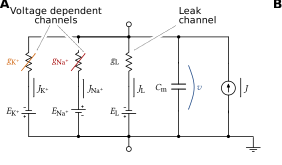
\includegraphics[scale=0.3333]{media/chapter_modelling_neurobiological_systems/hodgkin_huxley_circuit.pdf}~~~~\includegraphics{media/chapter_modelling_neurobiological_systems/action_potentials_hh_conductances.pdf}
	{\phantomsubcaption\label{fig:action_potentials_hh_conductances_circuit}}
	{\phantomsubcaption\label{fig:action_potentials_hh_conductances_conductances}}
	\vspace{-0.5cm}
	\caption[Equivalent circuit diagram of the Hodgkin-Huxley model]{Equivalent circuit diagram of the Hodgkin-Huxley model. \textbf{(A)} Equivalent circuit model of the Hodgkin-Huxley model. The resting potential is generated by a virtual \enquote{leak} channel; the $\mathrm{K}^+$ and $\mathrm{Na}^+$ channels vary over time and depend on the membrane potential. \textbf{(B)} Conductance traces for a single action potential (slice from \cref{fig:action_potentials_superthreshold}). Sodium drives depolarisation, potassium repolarisation.}
	\label{fig:action_potentials_hh_conductances}
\end{figure}

Conveniently, the Hodgkin-Huxley model is an extension of the equivalent cell-membrane circuit from the previous subsection (\Cref{fig:electrical_circuit}).
We just need to make two conceptual changes to account for the linear subthreshold and nonlinear superthreshold dynamics.

\subsubsection{Subthreshold dynamics}
To model the linear subthreshold dynamics, we simply add a capacitor with capacitance $C_\mathrm{m}$ to the circuit model.
This \emph{membrane capacitance}\index{neuron!membrane capacitance} is physically motivated by the cell membrane separating two electrically charged bodies.
Any such system inherently possesses capacitive properties.%
\footnote{To be clear, the membrane capacitance is not specific to the Hodgkin-Huxley model. In fact, this assumption preceded the Hodgkin-Huxley model by several decades (e.g., \cite{lapicque1907recherches}). We discuss the corresponding LIF neuron model first proposed by Lapicque later in this chapter.}
Given an input current $J(t)$, the sub-threshold dynamics can be described in terms of the following differential equation
\begin{align}
	\begin{aligned}
	\CMem \dot\vMem(t) &=
		  g_\mathrm{K^+} \bigl(E_\mathrm{K^+} - \vMem(t)\bigr)
		+ g_\mathrm{Na^+} \bigl(E_\mathrm{Na^+} - \vMem(t)\bigr)
		+ g_\mathrm{Cl^-} \bigl(E_\mathrm{Cl^-} - \vMem(t)\bigr) + J(t) \\ &=
	g_\mathrm{L} \bigl(\EL - \vMem(t)\bigr) + J(t) \,.
	\end{aligned}
\end{align}
The last term simplifies the dynamics using a \emph{leak conductance} \gL and \emph{leak potential} \EL that form a basic resistor-capacitance (RC) circuit (right half of \Cref{fig:action_potentials_hh_conductances_circuit}) with the time-constant $\tauMem = \CMem g_\mathrm{L}^{-1}$.
We have
\begin{align*}
	\gL &= g_\mathrm{K^+} + g_\mathrm{Na^+} + g_\mathrm{Cl^-} \,, &
	\text{and} \quad \quad \EL &= \frac{g_\mathrm{K^+} E_\mathrm{K^+} +
				 	g_\mathrm{Na^+} E_\mathrm{Na^+} + g_\mathrm{Cl^-} E_\mathrm{Cl^-}}{g_\mathrm{K^+} + g_\mathrm{Na^+} + g_\mathrm{Cl^-}} \,.
\end{align*}
The equation for \EL is exactly the equilibrium potential as per \cref{eqn:circuit_equilibrium_ions}.
In the absence of an input current $J(t)$, \EL is a stable attractor in the subtreshold dynamics.
It typically holds $\vRest = \EL$; still, we use \EL in this context to emphasise its use as a conductance-based channel.

\subsubsection{Superthreshold dynamics}
The superthreshold dynamics are responsible for action potential generation.
We describe these nonlinear dynamics in terms of potassium and sodium channels with time-dependent conductances $g_\mathrm{K^+}(t)$, $g_\mathrm{Na^+}(t)$ (\Cref{fig:action_potentials_hh_conductances_circuit}):
\begin{align*}
	\CMem \dot\vMem(t) &=
		  g_\mathrm{K^+}(t) \bigl(E_\mathrm{K^+} - \vMem(t)\bigr)
		+ g_\mathrm{Na^+}(t) \bigl(E_\mathrm{Na^+} - \vMem(t)\bigr)
		+ g_\mathrm{L} \bigl(\EL - \vMem(t)\bigr) + J(t) \,.
\end{align*}
Hodgkin and Huxley define the time-course of these conductances in terms of a dynamical system of gating variables $m(t)$, $h(t)$, and $n(t) \in [0, 1]$ that in turn depend on $\vMem(t)$.
We have
\begin{align*}
	g_\mathrm{K^+}(t) &= \hat g_\mathrm{K^+} n(t)^4 \,, &
	g_\mathrm{Na^+}(t) &= \hat g_\mathrm{Na^+} m(t)^3 h(t) \,,
\end{align*}
where $\hat g_\mathrm{K^+}$ and $\hat g_\mathrm{Na^+}$ are the maximum conductances.
%Using place-holder functions $f_m$, $f_n$, $f_h$, the dynamics of the gating variables are
%\begin{align*}
%	\dot m(t) &= f_m(v(t), m(t)) \,, &
%	\dot h(t) &= f_h(v(t), h(t)) \,, &
%	\dot n(t) &= f_n(v(t), n(t)) \,.
%\end{align*}
The dynamics of the gating variables (cf.~\Cref{app:hippocampal_hh}) produce a tight feedback loop between $\vMem(t)$ and the conductances.

\Cref{fig:action_potentials_hh_conductances_conductances} depicts the resulting conductances over time.
In particular, $g_\mathrm{Na^+}(t)$ rises rapidly once a certain threshold potential is exceeded.
This drives the cell towards the positive sodium reversal potential $E_\mathrm{Na^+}$; the cell becomes depolarised.
In turn, the positive membrane potential triggers a rise in potassium conductivity $g_\mathrm{K^+}(t)$, while the gating variable $h(t)$ shuts the sodium current off. This drives the cell towards the negative potassium reversal potential $E_\mathrm{K^+}$; the cell becomes hyperpolarised, while the potassium conductance remains relatively high for a short time.
This accounts for refractoriness, as large $J$ are required to counter the potassium current.

A detailed description of the superthreshold dynamics is provided in \Cref{app:hippocampal_hh}, including the unabridged equations and additional diagrams.
An even more thorough discussion of the dynamics of Hodgkin-Huxley-like neurons may be found in \citet{izhikevich2007dynamical}.

\subsection{Compartmental Neuron Models}

\begin{figure}
	\centering
	\includegraphics{media/chapter_modelling_neurobiological_systems/compartments.pdf}
	{\phantomsubcaption\label{fig:compartments_physical}}%
	{\phantomsubcaption\label{fig:compartments_volumes}}%
	{\phantomsubcaption\label{fig:compartments_circuit}}%
	\caption[Equivalent circuit of an exemplary compartmental neuron model]{Equivalent circuit diagram of an exemplary compartmental neuron model. \textbf{(A)} A biological neuron is divided into $N = 6$ individual compartments (neuron redrawn from \cite{howell1916textbook}, Figure~84, p.~187).
	\textbf{(B)} Compartments are often approximated as cylinders; using \enquote{cable theory} one can compute how potentials propagate along the membrane.
	\textbf{(C)} Cylinder models can be further simplified by modelling each compartment as a simple equivalent circuit. Here, the somatic compartment (orange) possesses Hodgkin-Huxley-like voltage-dependent dynamics. Individual model circuits are resistively coupled with conductances $g_{ij}$.
	}
	\label{fig:compartments}
\end{figure}

As we saw at the beginning of this section, neurons possess intricate morphologies (cf.~\Cref{fig:compartments_physical}).
Up to this point, we glanced over this fact and instead summarised neural electrophysiology in terms of a single membrane potential over time, $\vMem(t)$.
Models based on this assumption are referred to as \emph{point neurons} or \emph{single compartment models}.

The spatial organization of a neuron can have a significant impact on its function.
This is because the intracellular fluid is not a particularly good electrical
conductor.
Hence, in combination with the capacitive properties of the membrane, we can, at a single point in time, measure different membrane potentials throughout the neuron.
These voltage differences cause currents injected at different points of the neuron to interact nonlinearly, which supports computation.
Perhaps confusingly, the neural \emph{dynamics} we describe here are mostly linear, but the \emph{average effect over time} is nonlinear.
We discuss this in more detail in the next chapter.

\begin{figure}
	\includegraphics{media/chapter_modelling_neurobiological_systems/cylinder.pdf}
	\caption[Illustration of potential propagation within a cylindrical cable.]{Illustration of potential propagation within a cylindrical cable. Injecting a \SI{1}{\nano\ampere} current at the centre of a \SI{1}{\milli\metre} long cable (diameter \SI{1}{\micro\metre}, capacitance \SI{1}{\micro\farad\per\square\centi\metre}, longitudinal resistance \SI{150}{\ohm\per\centi\metre}, leak conductance \SI{0.5}{\milli\siemens\per\square\centi\metre}). \textbf{(A)} Potential at different points $x$ and times $t$ (see \emph{(B)} for a legend) in a linear cable. \textbf{(B)} Continuous representation of the same data; see \emph{(A)} for the mapping between colours and voltages.}
	\label{fig:cylinder}
\end{figure}

A quite faithful model of this can be constructed using \emph{cable theory}.
To this end, individual neurons are approximated as an arrangement of cylinders that represent individual segments of the neuron (\Cref{fig:compartments_volumes}).
Voltages spatially propagate through these cylinders. That is, the model takes the longitudinal resistance of the individual neuron segments as well as their capacitative properties into account.
Given an input impulse, we can use \emph{cable equations} to predict the voltage $v(x, t)$ at a certain position $x$ along the segment at a time $t$ (cf.~\Cref{fig:cylinder}).
Mathematically, this can be accomplished by assuming an infinite number of resistively coupled RC circuits and solving a partial differential equation \citep[Chapter~2]{koch1999biophysics}.


Instead of modelling spatial propagation of voltages through cylinders, individual cylinders can be approximated as one or multiple instances of the underlying equivalent circuit.
Each of these instances is referred to as a \emph{compartment} (\Cref{fig:compartments_circuit}).
Such neuron models are correspondingly called \emph{multi-compartment} or \emph{compartmental} neuron models.
In theory, the number of compartments $N$ determines how closely the model can be made to match empirical data---some detailed neuron models rely on thousands of individual segments.
However, for most network-level research, compartments can often be joined into reduced models that capture most of the original neural behaviour \citep{herz2006modeling}.

Depending on the modelling assumptions, compartments may either be \emph{active} or \emph{passive}.
Active compartments---such as the \enquote{somatic} compartment in \Cref{fig:compartments_circuit}---model superthreshold dynamics and are capable of producing spikes, for example by including voltage-dependent Hodgkin-Huxley type models.
In contrast, passive compartments are typically modelled as the simple linear subthreshold RC-circuit.
A more detailed description of such models, including the passive dendritic trees we discuss later, is given by \citet[Chapter~3]{koch1999biophysics}.

If we assume that individual neural compartments are resistively coupled, the current $J_i(t)$ flowing into the $i$th compartment is, according to Kirchhoff's circuit laws, given as
\begin{align}
	J_i(t) &= \sum_{j = 1}^N g_{ij} \bigl(v_j(t) - v_i(t)\bigr) \,.
	\label{eqn:multi_comp_current}
\end{align}
Here, $g_{ij} = g_{ji}$ is the conductance between the $i$th and $j$th compartment. A value of $g_{ij} = 0$ indicates no connection.
Mathematically, the conductances $g_{ij}$ correspond to the symmetric adjacency matrix of an undirected connectivity graph describing the compartmental model.

\section{From Individual Neurons to Spiking Neural Networks}
\label{sec:neuron_models}

The equations from the previous section model the basic electrophysiological properties of individual neurons.
Of course, a single neuron on its own does not give rise to animal behaviour.
Hence, in this section, we discuss how individual neurons form neural networks.
We provide an overview of synaptic transmission, the process underpinning neural information transfer, followed by a discussion 
idealised neuron and synapse models that lessen the computational burden of simulating biological systems.
We close with a short discussion of spiking neural networks and population tuning---the latter shedding some light onto the role that individual neurons play in a network.


\subsection{Synaptic Transmission}
\label{sec:synaptic_transmission}

So far, our descriptions of neural dynamics assumed that neurons receive inputs through artificially injected currents $J(t)$.
%While this can be experimentally achieved using a microelectrode and a precision power supply,
Of course, this does not explain how neurons receive inputs \emph{in vivo}.
As we mentioned in our overview in \Cref{sec:neurons_overview}, the interface between two neurons is called a \emph{synapse}.
Neuroscientists distinguish two synapse types: electrical and chemical.


\subsubsection{Electrical synapses}
In adult vertebrates, electrical synapses are significantly less common than chemical synapses.
Still, they play an important in some mammalian brain areas, including the retina and the inferior olive in the cerebellum \citep[Chapter~5]{meriney2019synaptic}.

Electrical synapses directly connect two neurons through specialised ion channels, so-called \emph{gap junctions}.
These channels typically allow a bidirectional exchange of ions between the intracellular fluids.
Correspondingly, neurons connected via gap junctions can be modelled using the same techniques as multi-compartment models (eq.~\ref{eqn:multi_comp_current}; \cite{kandel2012principles}, Chapter~8).

\subsubsection{Chemical synapses}
Neurons coupled via chemical synapses are electrically isolated.
The synapse establishes a unidirectional information flow and only passes on superthreshold signals.
We generally refer to the transmitting neuron as the \enquote{pre-neuron}, and to the receiving neuron as the \enquote{post-neuron}.
Similarly, the synapse is divided into the \enquote{pre-} and \enquote{post-synapse}.

\begin{figure}
	\includegraphics{media/chapter_modelling_neurobiological_systems/synapse.pdf}
	\caption[Synaptic transmission in a chemical synapse]{Synaptic transmission in a chemical synapse. Grey line in the membrane potential traces is the spike onset. See text for a description. Inspired by \citet[Figure~8-8B-C, p.~185]{kandel2012principles}.}
	\label{fig:synapse}
\end{figure}

As illustrated in \Cref{fig:synapse}, action potentials arriving at the \emph{synaptic bouton}, a bulbous protrusion of the pre-neuron axon terminal, triggers the release of \emph{neurotransmitter} molecules.
These traverse the nanometer-scale gap between the pre- and post-synapse, the \emph{synaptic cleft}, and temporarily bind to post-synaptic receptors specific to that neurotransmitter type.
This---directly or indirectly---causes ion channels in the post-neuron to open.
In turn, the permeability of the post-neuron for that particular ion species changes, influencing the membrane potential.

These synaptically mediated membrane potential fluctuations are called \emph{post-synaptic potentials} (PSPs).
Depending on the type of ion channels opened or closed, the PSP can either drive the neuron towards more positive voltages (if sodium channels are opened), or negative voltages (e.g., if potassium or chloride channels are opend).
Positive PSPs are referred to as \emph{excitatory} (EPSP), negative changes as \emph{inhibitory} (IPSP).
%Correspondingly, we distinguish excitatory and inhibitory post-synaptic potentials (EPSPs) and (IPSPs).

Whether a pre-neuron acts excitatorily or inhibitorily on a post-neuron depends on the kind of neurotransmitter released by the pre-neuron, as well as the specific receptors and ion channels in post-neuron.
%Typically, each neurotransmitter either has an inhibitory or excitatory effect.
For example, the Gamma-Aminobutyric acid (GABA) neurotransmitter is primarily inhibitory (via GABA\textsubscript{A} or GABA\textsubscript{B} receptors), whereas Glutamic acid (Glutamate) is mostly excitatory (via AMPA or NMDA receptors; \cite{kandel2012principles}, Chapter~10).

Importantly, the mixture of neurotransmitters is the same across all axonal branches of a neuron.
This is known as \emph{Dale's principle}\index{Dale's principle} \citep{strata1999dale,eccles1986chapter}.
Put simply, individual neurons typically either act excitatorily or inhibitorily on their post-neurons.%
\footnote{This characterisation of Dale's principle is useful, but technically incorrect. For example, a pre-synapse releasing glutamate typically excites post-neurons, but inhibits special neurons with inhibitory glutamate receptors \citep{cleland1996inhibitory}.
Additionally, synapses could release both excitatory and inhibitory neurotransmitters.
%Furthermore, Dale's principle solely states that the \emph{mixture} of neurotransmitters is uniform within the axonal branches of a neuron \citep{strata1999dale,eccles1986chapter}. In theory, the pre-synapse could release both excitatory and inhibitory neurotransmitters.
}
We hence refer to neurons---and not just individual synapses---as being excitatory or inhibitory.

\begin{figure}
	\centering
	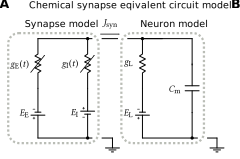
\includegraphics[scale=0.3333]{media/chapter_modelling_neurobiological_systems/synapse_model.pdf}%
	\includegraphics{media/chapter_modelling_neurobiological_systems/synapse_model_traces.pdf}%
	{\phantomsubcaption\label{fig:synapse_model_circuit}}%
	{\phantomsubcaption\label{fig:synapse_model_traces}}%
	\caption[The conductance-based synapse model]{The conductance-based synapse model.
	\textbf{(A)} Circuit diagram of a passive cell membrane with synaptically controlled excitatory and inhibitory conductance-based channels.
	\textbf{(B)} Illustrative voltage, current, and conductance traces. \emph{Top:} Excitatory and inhibitory channel conductances after a pre-synaptic action potential (grey dashed line). \emph{Middle:} Resulting excitatory and inhibitory post-synaptic potentials. \emph{Bottom:} Corresponding excitatory and inhibitory post-synaptic currents.}
	\label{fig:synapse_model}
\end{figure}

\subsubsection{Conductance-based chemical synapse model}
Most gated ion channels can be modelled as a voltage-resistor pair with variable conductance per receptor type \citep{roth2009modeling}.
This is depicted in \Cref{fig:synapse_model} for generic \enquote{excitatory} and \enquote{inhibitory} receptors.
Mathematically, the post-synaptic current $J_\mathrm{syn}(t)$ flowing from the synapse into the neuron is given as
\begin{align}
	J_\mathrm{syn}(t) &=
		  g_\mathrm{E}(t) \bigl(E_\mathrm{E} - v(t)\bigr)
		+ g_\mathrm{I}(t) \bigl(E_\mathrm{I} - v(t)\bigr) \,.
	\label{eqn:conductance_synapse}
\end{align}
Here, $E_\mathrm{E}$ and $E_\mathrm{I}$ are the equilibrium potentials of the gated ion channels.
These potentials are not necessarily equal to ion reversal potentials (\Cref{tbl:nernst}).
For example, NMDA and AMPA channels conduct both $\mathrm{Na^+}$ and $\mathrm{K^+}$, resulting in $E_\mathrm{E} \approx \SI{0}{\milli\volt}$ \citep[Chapter~10]{kandel2012principles}.
%All receptors with the same reversal potential are summarised as single channel in the equivalent circuit.
%Correspondingly, $g_\mathrm{E}$ and $g_\mathrm{I}$ are the sum over the state of multiple post-neurons (similar to \Cref{fig:electrical_circuit_individual_channels}).

\subsubsection{Synaptic dynamics and weights}
The time course of the conductance $g(t)$ depends on the neurotransmitter and receptor type.
Generally speaking, as illustrated in \Cref{fig:synapse_model_traces}, the conductance rises quickly after a spike is received, and decays slowly as the neurotransmitter unbinds from the receptors.
Receptors directly controlled by neurotransmitters acting as ligands (\Cref{fig:synapse}) tend to have relatively short time-constants between $1$ and \SI{100}{\milli\second} \citep{jones2014neurotransmitter}.
Some receptors (e.g., \enquote{metabotropic receptors}) rely on indirect chemical cascades, leading to longer time-constants \citep[Chapter~14]{meriney2019synaptic}; this is not captured well by the models we present here \citep{roth2009modeling}.

\begin{figure}
	\includegraphics{media/chapter_modelling_neurobiological_systems/synapse_filter_examples.pdf}
	{\phantomsubcaption\label{fig:synapse_filter_examples_time_constants}}%
	{\phantomsubcaption\label{fig:synapse_filter_examples_traces}}%
	\caption[Second- and first-order exponential synaptic low-pass filter dynamics]{Illustration of the second- and first-order exponential synaptic low-pass filter dynamics. \textbf{(A)} Impulse response of the second-order dynamics for different $\tau_1$ and $\tau_2$. \emph{Top:} visualisation of the time-constants used below. Swapping $\tau_1$ and $\tau_2$ does not change the dynamics (grey crosses). \emph{Bottom:} Impulse response of the filters (responses normalised to equal area), circles are the peaks. \textbf{(B)} Illustration of post-synaptic conductance traces (\emph{bottom}) according to \Cref{eqn:low_pass_second_order,eqn:low_pass_first_order} for two pre-neurons producing action-potentials (\emph{top}) connected with two different synaptic weights $w_1$, $w_2$.}
\end{figure}

Ligand-gated receptor dynamics are often modelled as a second-order linear dynamical system.
Let $t_{ij}$ denote the time of the $j$th pre-synaptic spike arriving from the $i$th pre-neuron, and let $\tau_1$, $\tau_2$ denote the rise and delay times (\Cref{fig:synapse_filter_examples_time_constants}).
We have \citep{roth2009modeling}:
\begin{align}
	\dot g_1(t) &= -\frac{g_1(t)}{\tau_\mathrm{1}} + g_2(t) \,, &
	\dot g_2(t) &= -\frac{g_2(t)}{\tau_\mathrm{2}} + \sum\nolimits_{i} \alpha w_i \sum\nolimits_{j} \delta(t_{ij} - t) \,,
	\label{eqn:low_pass_second_order}
\end{align}
where $\delta(t)$ is the Dirac-delta, and $\alpha$ is a scaling factor such that the scalar $w_i$ corresponds to the peak value of $g_1(t)$ for a single action potential received from pre-neuron $i$ (\Cref{fig:synapse_filter_examples_traces}).
For $\tau_1 = \tau_2$ this type of synaptic dynamics follow the so-called \emph{alpha function}.

Notably, the scalar $w_i$ is referred to as \emph{synaptic weight} in computational modelling, or as \emph{synaptic strength} in neuroscience.
This scalar summarises various biological processes that determine the average response of the post-neuron to an action-potential received from the $i$th pre-neuron.
For example, synaptic strength can depend on the amount of neurotransmitter released in the pre-synapse, or the ion-channel density in the post-synapse \citep[Chapter~12]{kandel2012principles}.
In this context, the term \emph{synaptic plasticity} refers to a change in synaptic strength over time.
This plays a key role in learning---we discuss this in more detail in Chapter~5.


Typically, the rise-time of $g(t)$ is relatively short.
Correspondingly, the second-order low-pass filter can be approximated by a first-order dynamical system with decay-time $\tau$.
Mathematically, and as depicted the lower portion of \Cref{fig:synapse_filter_examples_traces}, the dynamics are
\begin{align}
	\dot g(t) &= -\frac{g(t)}{\tau} + \sum\nolimits_{i}  w_i \sum\nolimits_{j} \delta(t_{ij} - t) \,.
	\label{eqn:low_pass_first_order}
\end{align}

\subsubsection{Synaptic dynamics as filters}
The above synaptic dynamics (eqs.~\ref{eqn:low_pass_second_order}, \ref{eqn:low_pass_first_order}) are linear time-invariant (LTI) systems.
%of the form $\dot{\vec g}(t) = \mat A{\vec g(t)} + \mat B u(t)$, where $\mat A \in \mathbb{R}^{n \times n}$ is a state-transition matrix, $\mat B \in \mathbb{R}^{n \times 1}$ is the input matrix, and $u(t)$ is the input in the form of weighted pre-synaptic spike events; the output of the system (i.e., the conductance) is simply the first state-dimension $g_1$.
LTI systems are fully characterised by their \emph{impulse response} $h(t)$ and can be replaced by a convolution (\enquote{$\ast$}) between $h(t)$ and the weighted input spike-train $u(t)$:
\begin{align}
	g(t)
		&= (h \ast u)(t)
		 = \int_0^t h(\tau) u(\tau - t) \,\mathrm{d}\tau
		 = \int_0^t h(\tau) \sum\nolimits_{i}  w_i \sum\nolimits_{j} \delta(t_{ij} - \tau) \,\mathrm{d}\tau \,.
	\label{eqn:synapse_impulse}
\end{align}
For the first-order dynamics in \cref{eqn:low_pass_first_order}, the impulse response is $h(t) = \exp(-t/\tau)$ for $t \geq 0$ (and $h(t)= 0$ if $t < 0$); impulse responses of the second-order system are depicted in \Cref{fig:synapse_filter_examples_time_constants}.
Convolutions such as \cref{eqn:synapse_impulse} can alternatively be expressed as multiplication of the frequency contents of the impulse response $h(t)$ and the input spike-train $u(t)$:
\begin{align}
	g(t) &= \mathcal{F}^{-1} \bigl(\mathcal{F}(h) \mathcal{F}(u) \bigr)(t) \,,
\end{align}
where $\mathcal{F}$ is the forward Fourier transformation, and $\mathcal{F}^{-1}$ its inverse.
From this signal-processing perspective, the synaptic dynamics attenuate frequencies in the input spike-train; they act as a \emph{filter}.
The synaptic dynamics discussed so far attenuate low frequencies far less than higher frequencies; they are thus referred to as \emph{low-pass filters}.

% TODO: Talk about filters in general
% TODO: Provide some example synaptic time constants

\newpage

\subsection{Simplified Neuron Models}
\label{sec:simplified_neuron_models}

The models discussed in the previous section describe indiviudal neurons at a relatively low level of abstraction.
This incurs a high computational cost, especially when considering detailed compartemental neurons with Hodgkin-Huxley-like super-threshold dynamics.

Fortunately, important electrophysiological properties of neurons can be captured by less detailed, computationally inexpensive, models \citep[cf.][Chapter~14]{koch1999biophysics}.
For example, the Izhikevich \citep{izhikevich2004which} and Adaptive Exponential \citep{brette2005adaptive} point neuron models require only two state variables, but are capable of reproducing spike patterns observed in nature.
Here, we focus on the even simpler \enquote{leaky integrate-and-fire} model\index{leaky integrate-and-fire model} (LIF).

\subsubsection{The leaky integrate-and-fire model}

\begin{figure}[t]
	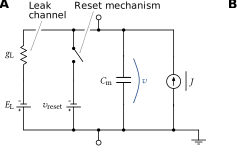
\includegraphics[scale=0.3333]{media/chapter_modelling_neurobiological_systems/lif_circuit.pdf}%
	\kern-0.25cm\includegraphics{media/chapter_modelling_neurobiological_systems/lif_traces.pdf}
	\caption[Equivalent circuit diagram and membrane potential trace of a LIF neuron]{Equivalent circuit diagram and membrane potential trace of a LIF neuron. \textbf{(A)} The LIF model consists of a capacitative membrane with a \enquote{leak} channel. A reset mechanism clamps \vMem to the reset potential \vReset. \textbf{(B)} Membrane potential trace (\emph{top}) for rectangle pulse current inputs (\emph{middle}).  Vertical dashed lines are spike events. The bottom graph depicts the remaining refractory period.}
	\label{fig:lif}
\end{figure}

%\footnote{Extensions to the LIF model include the quadratic and exponential integrate-and-fire models (QIF and EIF, respectively). Hence, LIF is sometimes read as \enquote{linear integrate-and-fire}. Furthermore, there is the IF model, that does not include a leak channel, sometimes also called nLIF (non-leaking).}
A variant of the LIF model---lacking refractoriness---dates back to \citet{lapicque1907recherches}.
Just like the Hodgkin-Huxley model (\Cref{sec:neural_dynamics}), the LIF neuron is based on a capacitive membrane with a leak channel.
The input current is integrated by the capacitor, which, at the same time, is discharged through the leak channel:
\begin{align}
	\CMem \dot{\vMem}(t) =
		\gL \bigl(\EL - \vMem(t)\bigr) + J(t) \,,
	\label{eqn:lif}
\end{align}
where \gL is the leak conductance, \EL is the leak reversal potential, and $J(t)$ is a (synaptic) current injected into the membrane.
Unlike the Hodgkin-Huxley model, the dynamics of the system do not model spike production; \enquote{firing} is handled outside the dynamical system. 
Once $\vMem(t)$ reaches a threshold $\vTh$, a spike event is recorded and \vMem is held at the \emph{reset potential} \vReset for the duration of the refractory period \tauRef.
This is depicted in \Cref{fig:lif}.

\subsubsection{Response curve}

\begin{figure}
	\centering
	\includegraphics{media/chapter_modelling_neurobiological_systems/neuron_voltage_traces.pdf}
	\caption[Voltage traces for the LIF and Hodgkin-Huxley neuron model]{Voltage traces (\emph{top}) for the LIF and a Hodgkin-Huxley-type neuron dynamics described by \citet{traub1991neuronal} given a current ramp input~(\emph{bottom}). Dashed vertical lines correspond to spike events. Dotted line is the resting potential at $\EL=\SI{-65}{\milli\volt}$. Both neurons have a membrane capacitance of $C_\mathrm{m} = \SI{200}{\pico\farad}$ and a leak conductance of $g_\mathrm{L} = \SI{10}{\nano\siemens}$. \textbf{(A)} The LIF neuron model does not account for spike production; the voltage is simply reset to $v_\mathrm{reset} = \SI{-85}{\milli\volt}$ for $\tauRef = \SI{2}{\milli\second}$ once the membrane potential passes the threshold at $v_\mathrm{th} = -\SI{55}{\milli\volt}$. \textbf{(B)} Same experiment for a Hodgkin-Huxley neuron. Notably, the super-threshold dynamics of the Hodgkin-Huxley model action potentials and the first spike appears significantly earlier compared to the LIF neuron.}
	\label{fig:neuron_voltage_traces}
\end{figure}

\begin{figure}
	\centering
	\includegraphics{media/chapter_modelling_neurobiological_systems/neuron_response_curves.pdf}%
	{\phantomsubcaption\label{fig:neuron_response_curves_lif}}%
	{\phantomsubcaption\label{fig:neuron_response_curves_hh}}%
	\caption[Response curves for the LIF and Hodgkin-Huxley neuron model]{Response curves (also called IF-curves) $G[J]$ for the LIF and Hodgkin-Huxley neuron model from \Cref{fig:neuron_voltage_traces}. Data extracted from the inter-spike-intervals of a current ramp experiment (sweep from \SIrange{0}{2}{\nano\ampere} over ten seconds at a \SI{10}{\micro\second} resolution). Although the LIF and Hodgkin-Huxley models have drastically different dynamics, their response curves are qualitatively similar.}
	\label{fig:neuron_response_curves}
\end{figure}

\begin{figure}
	\centering
	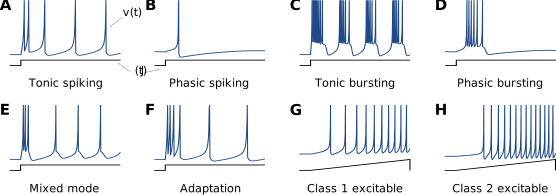
\includegraphics{media/chapter_modelling_neurobiological_systems/izhikevich_whichmod_figure1.pdf}%
	{\phantomsubcaption\label{fig:izhikevich_whichmod_figure1a}}%
	{\phantomsubcaption\label{fig:izhikevich_whichmod_figure1b}}%
	{\phantomsubcaption\label{fig:izhikevich_whichmod_figure1c}}%
	{\phantomsubcaption\label{fig:izhikevich_whichmod_figure1d}}%
	{\phantomsubcaption\label{fig:izhikevich_whichmod_figure1e}}%
	{\phantomsubcaption\label{fig:izhikevich_whichmod_figure1f}}%
	{\phantomsubcaption\label{fig:izhikevich_whichmod_figure1g}}%
	{\phantomsubcaption\label{fig:izhikevich_whichmod_figure1h}}%
	\caption[Diversity of neural dynamics for constant or ramp input currents]{Diversity of neural dynamics for constant or ramp input currents. Each plot depicts membrane-potential traces $v(t)$ (\emph{top}) of the Izhikevich neuron model (with different parameters) for an input current $J(t)$ (\emph{bottom}). LIF neurons are only capable of behaviours \emph{A} and \emph{G}. Partially reproduced (dynamics for input pulses were skipped) with minor modifications from \citet{izhikevich2004which}. Electronic version of the figure and reproduction permissions freely available at \url{http://www.izhikevich.org}.}
	\label{fig:izhikevich_whichmod_figure1}
\end{figure}

\Cref{fig:neuron_voltage_traces} depicts a comparison between the Hodgkin-Huxley and the LIF dynamics.
The reset and threshold potential of the LIF neuron model have been tuned to match the sub-threshold membrane potentials observed in the Hodgkin-Huxley neuron.
In both cases---apart from the obviously missing super-threshold dynamics---the inter-spike-interval decreases the larger $J$, leading to a higher spike rate.
This suggests a characterisation of neurons in terms of their \emph{response curve}\index{neuron!response curve} $G[J]$ (\Cref{fig:neuron_response_curves})
\begin{align}
	G[J] &= \lim_{T \to \infty} \frac{n_\mathrm{spikes}(J, T)}{T} \,, & \text{where } n_\mathrm{spikes}(J, T) &= \text{\#spikes for input $J$ over a period $T$} \,.
	\label{eqn:response_curve}
\end{align}
Of course, this only makes sense if we assume that the neuron has a non-zero steady-state activity for a constant superthreshold input current.
This is not necessarily true; neurons can exhibit complex behaviours that violate this assumption \citep{izhikevich2004which}.
For example, \emph{phasic} neurons only produce a limited number of spikes in response to an input step (Figure~\ref{fig:izhikevich_whichmod_figure1}B, D, E), while other neurons adapt to constant input currents over time, resulting in a reduction in frequency (Figure~\ref{fig:izhikevich_whichmod_figure1}F).
Still, neurons often behave \emph{tonically} (Figure~\ref{fig:izhikevich_whichmod_figure1}A, C, G, H), and can be reasonably well characterised in terms of a response curve.

Response curves and time-less \enquote{rate neurons} form the basis for artificial neural networks commonly used in machine learning. We discuss this in more detail later in this thesis.
Furthermore, we revisit temporal properties of the response curve when we discuss temporal tuning curves. % LEAVE SPACE HERE
% TODO add section references

\subsubsection{LIF response curve}
For most neuron models, it is impossible to derive a closed-form expression for the average spike rate $G[J]$ given a constant current $J$; there typically is no closed-form solution for $G[J]$. 
%\footnote{Very few differential equations posses closed-form solutions. Even slightly more complex models (e.g.,~first-order current-based synapses instead of constant $J$) require the analytic Lambert $\mathcal{W}$ function in the solution.}
Instead, we have to rely on the method suggested by \cref{eqn:response_curve}.
That is, we simulate the neural dynamics for a sufficiently long time-period and count the number of spikes $n_\mathrm{spikes}$.

The LIF neuron is a notable exception to this, as its subthreshold dynamics form a simple first-order linear dynamical system.
Using basic techniques for solving differential equations, the membrane potential \vMem at time $t$ for a constant input current $J$ is given as
\begin{align}
	v(t) &= \left(1 - e^{-\frac{t}{\tauMem}} \right) \left( \EL + \frac{J}{\gL} \right) + e^{-\frac{t}{\tauMem}} v(0) \,, &&\Rightarrow & \lim_{t \to \infty} v(t) &= \EL + \frac{J}{\gL} \,.
\end{align}
To compute the average spike rate, we need to know how long it takes to reach the threshold potential after a spike has been issued.
To this end, we simply solve $v(t_\mathrm{spike}) = \vTh$ with $v(0) = \vReset$ for $t_\mathrm{spike}$.
Keeping in mind that the neuron is held at the reset potential for $\tauRef$ seconds after every spike, and defining the threshold current $J_\mathrm{th} = (\vTh - \EL) \gL$, we have
\begin{align}
	\begin{aligned}
	G[J] &= \begin{cases}
		0 & \text{if } J \leq J_\mathrm{th} \,, \\
		\frac{1}{\tauRef + t_\mathrm{spike}} & \text{if } J > J_\mathrm{th} \,,
	\end{cases} & \quad
	\text{where }
%	J_\mathrm{th} &=
%		(\vTh - \EL) \gL \,, \\
	t_\mathrm{spike} &=
		-\tauMem \log\left(1 - \frac{(\vTh - \vReset) \gL}{(\EL - \vReset) \gL + J} \right) \,.
	\end{aligned}
	\label{eqn:lif_response_curve}
\end{align}
As depicted in \Cref{fig:neuron_response_curves_lif}, the predicted rate perfectly matches the empirical measurement.
Notably, the LIF response curve is qualitatively similar to that of the Hodgkin-Huxley neuron (\Cref{fig:neuron_response_curves_hh})---surprisingly so, as the dynamical systems differ wildly between the two models.
This makes LIF neurons a reasonable choice for simulating large-scale neurobiological systems at small computational costs (\cite{meunier2002playing}).

\subsubsection{Simplified LIF neuron}
A qualitatively equivalent form of the LIF neuron is given by normalising the voltages such that $\EL = 0$ and $\vTh = 1$, and furthermore setting $J_\mathrm{th} = 1$:
\begin{align}
	\dot v(t) &= -\frac{1}{\tauMem} v(t) + J(t) \,, &
	G[J] &= \begin{cases}
		0 & \text{if } J \leq 1 \,, \\
		\frac{1}{\tauRef - \tauMem \log\left(1 - \frac{1 - \vReset}{J-\vReset}\right)} & \text{if } J > 1 \,.
	\end{cases}
	\label{eqn:lif_simplified}
\end{align}
The primary advantage of this form is the reduction in mathematical operations compared to \cref{eqn:lif}.
This simplification is thus (among other tricks) exploited by the neural network simulator \enquote{Nengo} to support large-scale spiking neural network simulations \citep{bekolay2014nengo}.
The downside is a reduced interpretability of the now unit-less $v(t)$ and $J(t)$.

\subsubsection{Current-based synapse models}
Another possible simplification---both in terms of computation and mathematical analysis---concerns the synapse model.
In conductance-based synapses (\Cref{sec:synaptic_transmission}) the current $J_\mathrm{syn}(t)$ explicitly depends on the membrane potential $\vMem(t)$.
Going back to \Cref{fig:synapse_model_traces}, one may notice that the post-synaptic currents can be approximated as a scaled version of the conductance \citep[cf.][]{roth2009modeling}.

This suggests modelling the post-synaptic current $J_\mathrm{syn}$ as a linear superposition of filtered spike events.
Let the synaptic weight $w_i$ denote the peak post-synaptic current.
Then, the first-order \emph{current-based} synapse model is given as (analogously for higher-order filters)
\begin{align}
	\dot J_\mathrm{syn}(t) &= -\frac{J_\mathrm{syn}(t)}{\tau} + \sum\nolimits_{i}  w_i \sum\nolimits_{j} \delta(t_{ij} - t) \,.
	\label{eqn:low_pass_first_order_current}
\end{align}
We compare conductance- and current-based synapse models in more detail in the next chapter.

\pagebreak

\subsection{Spiking Neural Networks}
\label{sec:neural_codes}

\begin{figure}
	\centering
	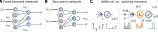
\includegraphics{media/chapter_modelling_neurobiological_systems/neural_networks.pdf}%
	{\phantomsubcaption\label{fig:neural_networks_a}}%
	{\phantomsubcaption\label{fig:neural_networks_b}}%
	{\phantomsubcaption\label{fig:neural_networks_c}}%
	\caption[Illustration of different neural network types]{Illustration of different neural network types. Blue circles depict individual neurons. \textbf{(A)} Feed-forward neural networks can be represented as acyclic graphs. \textbf{(B)} If the network connectivity contains cycles (e.g., the 5-2-4-5 cycle), the network is called \emph{recurrent}. Cycles can also be self-recurrences (e.g., neuron 6). \textbf{(C)} Artifical neurons (\emph{left}) process time-discrete samples. Spiking neurons (\emph{right}) are time-continous; they receive a weighted input spike train, filter it, and produce an output spike train.}
\end{figure}

% How to build neural networks
% Define feed-forward and recurrent neural networks
% But how to select the weights?
% Solution that artificial neural networks do
% But is this what biology does?
% Rate vs temporal coding debate -> Aaron

We are now well-equipped to construct and simulate spiking neural networks (SNNs).
In theory, we just take $n$ spiking neurons and connect them up according to synaptic weights $w_{ij}$. As mentioned before, these weights determine the connection strength between a pre-neuron $j$ and post-neuron $i$. Inputs are additive over multiple pre-neurons (eqs.~\ref{eqn:low_pass_first_order}, \ref{eqn:low_pass_first_order_current}).%
\footnote{This notion of synaptic weights $w_{ij}$ assumes that each neuron possesses a single synaptic input channel.
Hence, there is only a single synaptic weight matrix.
For neurons with multiple synaptic input channels we can simply use an individual weight matrix for each input channel. We discuss this in the next chapter.}

Mathematically, the \emph{weight matrix} $\mat W \in \mathbb{R}^{n \times n}$ is the adjacency matrix of a directed connectivity graph.%
\footnote{For convenience and computational efficiency, neurons are typically grouped into \enquote{layers}, \enquote{populations}, or \enquote{ensembles} (all terms are used synonymously).
Not all layers have connections among each other. Hence, $\mat W$ typically is a block-matrix that can be split into multiple sub-matrices.}
Networks with acyclic connectivity are called \emph{feed-forward} (\Cref{fig:neural_networks_a}); networks with cyclic connectivity are \emph{recurrent} (\Cref{fig:neural_networks_b}).
Feed-forward SNNs have finite memory.
Assuming plausible synaptic filters, their impulse response decays exponentially.
In contrast, and as we discuss later, recurrent networks can posses more interesting dynamics.

To actually simulate an SNN, we feed an external input (e.g., a set of currents or spike-trains) into the network and numerically integrate the coupled differential equations.
There are numerous general-purpose simulator software packages that do this efficiently, e.g., NEST \citep{gewaltig2007nest}, Brian \citep{stimberg2019brian}, GeNN \citep{yavuz2016genn}, or Nengo \citep{bekolay2014nengo}.

The most important question---and one that we pursue for the remainder of this thesis---is how to ultimately select $\mat W$.
For the artificial neural networks (ANNs) used in machine learning (\Cref{fig:neural_networks_c}), the astoundingly successful answer is to use stochastic gradient descent on a loss function $E$, i.e., $\dot{\mat W} = -\eta \nabla_{\mat W} E(\vec a_k, \vec {\hat a_k})$, where $\eta$ is a learning rate, $\vec a_k$ is the desired output activity for an input sample $\vec x_k$, and $\vec{\hat a_k}$ is the actual output \citep{lecun2015deep}.
For example, one common choice for the loss function is $E(\vec a_k, \vec {\hat a_k}) = \|\vec a_k - \vec{\hat a}_k\|^2$.

Similar gradient-descent global optimisation methods can be applied in the context of SNNs as well.
\Citet{hunsberger2018spiking} characterises the LIF response curve $G[J]$ in a network context and then trains an ANN that uses $G[J]$ as a nonlinearity.
The resulting $\mat W$ can then be used in a spiking context.
\Citet{goltz2020fast} optimise synaptic weights such that desired spike-timings are generated by a black-box spiking neural network simulator.

%Computational neuroscientists often distinguish between rate and temporal spike-codes, though the definitions of these concepts are quite vague.
%For example, \citet[Chapter~1]{gerstner2002spiking} list three different definitions of the term \enquote{rate code}, while \citet{abbott2001theoretical} list four definitions.
%Rates are estimated by either binning and counting, causal and acausal filtering, or (orthogonally) taking averages over entire populations into account.

%A similar zoo of definitions is to be had for temporal codes. For example, as pointed out by \citet[Chapter~14]{koch1999biophysics}, researchers often interpret temporal codes as correlations between spike times carrying information (i.e., spikes from different pre-neurons arriving earlier or later relative to each other).
%Another popular temporal code is \enquote{time-to-first-spike}, i.e., the notion that neurons rely on the time between some synchronisation event and the first received spike event \citep{vanrullen2005spike}.

Notably, such global optimisation methods can be useful when modelling neurobiological systems.
For example, there are striking similarities between the neural tuning observed in visual cortex and the learned tuning of neurons in hierarchical image classification networks \citep{yamins2016using}.
However, this is, to some degree, accidental, and not explicitly imposed.
As we discussed at the beginning of this chapter, it is desirable build models that reliably adhere to certain constraints---such as the aforementioned tuning properties.

\subsection{Neural Tuning and Population Codes}
\label{sec:neural_tuning}

\begin{figure}
	\centering
	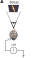
\includegraphics{media/chapter_modelling_neurobiological_systems/visual_cortex_tuning_setup.pdf}%
	\includegraphics{media/chapter_modelling_neurobiological_systems/visual_cortex_tuning.pdf}
	\caption[Neural tuning in the visual cortex]{Neural tuning in the visual cortex.
	\textbf{(A)} Illustration of the original experiment by \citet{hubel1959receptive}. Bright rectangles are briefly presented on a dark screen to an animal while recording from a neuron in its visual cortex. \textbf{(B)} Recorded spike trains for different stimulus orientations. Horizontal lines are the stimulus presentation interval. Adapted from \citet[Figure~3]{hubel1959receptive}. \textbf{(C)} The mapping between stimulus $\vec x$ and activity $a$ forms a \emph{tuning curve}. This neuron is tuned to vertical bars.}
	\label{fig:visual_cortex_tuning}
\end{figure}

%Given that we can simulate large biological systems at different levels of abstraction, the primary challenge is to construct networks that actually give rise to the behaviours observed in nature.
%Unfortunately, in many cases, too much about the brain is still unknown to successfully build such models.
%This is particularly true for brain regions involved in higher level cognition, and that, in terms of connectivity, are farther away from the periphery.
%Fortunately, brain regions \emph{closer} to the periphery are, relatively speaking, quite well understood.
%\footnote{Neuroscience textbooks such as \citet{kandel2012principles} discuss the neural circuitry of brain regions involved in sensory and motor processing in great detail, while chapters concerning higher-level cognitive tasks mostly report behavioural observations and coarse measurements such as fMRI scans.}
There are two important concepts that shed some light onto the organisation of brain networks---at least those brain networks involved in sensory processing: \emph{tuning curves} and \emph{receptive fields}.
In turn, these ideas motivate \emph{population codes}, which we heavily rely on in the context of our modelling tool, the Neural Engineering Framework---we discuss this in the next section.

\subsubsection{Tuning curves}
%Early studies on these concepts were conducted by \citeauthor{hubel1959receptive}.
In a famous \citeyear{hubel1959receptive} experiment (cf.~\Cref{fig:visual_cortex_tuning}), Hubel and Wiesel present a visual stimulus in the form of a bright rectangle at different orientations $\varphi$ to an experimental animal.
At the same time, the activity of a neuron in the animal's visual cortex is recorded.
This characterizes how the stimulus propagates through the brain up to the recording site.
%We characterize neurons in terms of their own physiological properties \emph{and} in terms of the preceding network connectivity.

In the recording depicted in \Cref{fig:visual_cortex_tuning}, we find that the neuron is most sensitive to---or, \emph{tuned} to---a certain orientation $\varphi$.
We could say that in this specific case, vertical bars the \emph{preferred direction} of the neuron.
Generally, such a mapping from a stimulus property $\varphi$ onto the average neural activity $a(\varphi)$ is called a \emph{tuning curve} \citep[e.g.,][p.~1112]{vandenbos2015apa}\index{neuron!tuning curve}\index{tuning curve}.

\subsubsection{Receptive fields}

\begin{figure}
	\centering
	\includegraphics{media/chapter_modelling_neurobiological_systems/gabor_filters.pdf}
	\caption[Examples of randomly generated of Gabor filters]{Examples of randomly generated Gabor filters.
	Each filter is a two-dimensional function $e(\xi_1, \xi_2)$, where $(\xi_1, \xi_2)$ is a spatial location.
	Negative  values (red) indicate that neural activity is reduced if a stimulus is present at that location, positive values (blue) indicate an increase in activity.}
	\label{fig:gabor}
\end{figure}
The concept of \emph{receptive fields}\index{neuron!receptive field}\index{receptive field} is closely related to tuning curves.
This is best illustrated in the context of stimuli that can be described as an intensity over a two-dimensional surface---such as vision or touch.
Generally, the receptive field of a neuron is the collection of points $(\xi_1, \xi_2)$ at which the presence of a stimulus---a point of light or mechanical pressure---triggers a neural response.
However, as evidenced by \citet{hubel1962receptive}, neural receptive fields are not only characterised in terms of the locations where a stimulus \emph{increases} the average neural activity, but also where the presence of a stimulus \emph{decreases} activity.

Mathematically, we can describe this in terms of a function $e(\xi_1, \xi_2)$ that assigns a weight to each stimulus location $(\xi_1, \xi_2)$.
This function $e$ is the receptive field.
\emph{Gabor filters}\index{Gabor filter} are a class of mathematical functions that fit observed receptive fields in the visual cortex well \citep{marcelja1980mathematical,field1986structure}.%
\footnote{Gabor filters are sinusoidals scaled by a radial Gaussian envelope. Such functions are maximally localised in time and space, as pointed out in the context of Gabor's Fourier uncertainty principle \citep{gabor1946theory}.}
Examples are depicted in \Cref{fig:gabor}.

Borrowing some notation from the next section, the activity of the neuron $a(x)$ can be modelled as the product between the receptive field $e$ and the stimulus $x$ integrated over space (where $x(\xi_1, \xi_2)$ is a function describing the stimulus intensity at a certain location)
\begin{align}
	a(x) &= G\left[ \alpha \iint e(\xi_1, \xi_2) x(\xi_1, \xi_2) \,\mathrm{d}\xi_1\mathrm{d}\xi_2 + \beta \right]
		= G \bigl[ \alpha \langle e, x \rangle + \beta \bigr] \,.
	\label{eqn:tuning_curve_from_receptive_field}
\end{align}
Here, $\langle e, x \rangle$ is the inner product between the receptive field and the stimulus (see \Cref{app:functional_analysis} for an introduction to functional analysis and the corresponding definitions).
Furthermore, $G$ is a rate approximation of the neuron model (see previous subsection), and, $\alpha > 0$ and $\beta$ translate the inner product into a neural input current.

Importantly, if the stimulus and receptive field are normalised, then $\langle e, x \rangle$ is the cosine similarity between the two functions.
Correspondingly, according to the above model, the neural response is maximised if $e = x$.
In other words, the receptive field \emph{is} the \enquote{true} preferred stimulus of a neuron.
This is consistent with modern definitions of the term \enquote{receptive field} in the neuroscience literature \citep[cf.][]{troy2009retinal}.

\begin{figure}
	\centering
	\includegraphics{media/chapter_modelling_neurobiological_systems/visual_cortex_receptive_field_example.pdf}
	\caption[Model of the Hubel and Wiesel experiment]{Model of the original Hubel and Wiesel experiment (cf.~\Cref{fig:visual_cortex_tuning}). \textbf{(A)} The receptive field $e(\xi_1, \xi_2)$ describes whether a stimulus location $(\xi_1, \xi_2)$ acts excitatory (blue), or inhibitory (red). \textbf{(B)} The stimulus is a light rectangle at different orientations $\phi$; this can be described as function $x$ mapping locations onto light intensity. \textbf{(C)} Tuning curve obtained according to the model in \cref{eqn:tuning_curve_from_receptive_field}.}
	\label{fig:visual_cortex_receptive_field_example}
\end{figure}

\Cref{fig:visual_cortex_receptive_field_example} illustrates the relationship between the receptive field of a neuron and one of its tuning curves.
Choosing a vertically oriented Gabor filter as a receptive field, we can model the orientation tuning from the original Hubel and Wiesel experiment.
Thus, in a nutshell, a tuning curve is a characterisation of the neuron in terms of a specific stimulus property (e.g., the orientation of a bar of light), whereas the receptive field models its tuning properties in general (e.g., the predicted activity for any visual stimulus).

\subsubsection{Population codes}
Although tuning curves and receptive fields are inherently reconstructed from a network context, they still only characterise individual neurons.
To better understand biological neural networks, we need to consider the tuning properties of groups of neurons.

Doing this, we find that neighbouring neurons often have similar tuning properties---they are tuned to the same sensory modality, and possess similar receptive fields \citep{berkowitz2009population}.
Again, this has been explored well in context of orientation tuning in the visual cortex \citep[Chapter~25]{kandel2012principles}.
For example, neurons in visual cortex are organised in \enquote{cortical columns}.
Each column consists of several layers of neurons.
Within a single layer of the same column, neurons possess the similar preferred orientations.
Between columns, preferred orientations differ significantly.

This, as well as several other observations \citep{yuste2015neuron}, suggest that brain networks use \emph{population codes}.
The idea is that a single underlying quantity---such as the orientation of a visual stimulus---is represented by a group of neurons in a distributed manner.
The opposite would be \enquote{single-neuron coding}, where the activity of individual, localised neurons maps onto some quantity, or, in higher-level cognition, onto specific concepts \citep{berkowitz2009population}.

\begin{figure}
	\centering
	\includegraphics{media/chapter_modelling_neurobiological_systems/population_code.pdf}
	\caption[Probabilistic decoding of scalar quantities using population codes]{Probabilistic decoding of scalar quantities using population codes.
	\textbf{(A)} \emph{Left:} The activity $a$ of a single neuron represents a scalar value $x \in [-1, 1]$.
	The current $J$ fed into each neuron is subject to Gaussian noise with standard deviation $\sigma = \SI{1}{\nano\ampere}$.
	Solid line corresponds to the median activity for the given represented value; shaded area corresponds to a contour line of the underlying probability density.
	\emph{Right:} Trying to decode the represented value $x$ from the activity results in significant uncertainties; negative values cannot be disambiguated. Dotted line is the optimum; solid line the median of a maximum-likelihood estimate, shaded area a contour line of the underlying probability density.
	Error $E$ is the decoding RMSE.
	\textbf{(B, C, D)} The larger the number of neurons, the smaller the uncertainties.}
	\label{fig:population_code}
\end{figure}

Population codes are intriguing as a model for representation in biological networks.
They allow precise inferences from imprecise or ambiguous observations. This is illustrated in \Cref{fig:population_code}.
For example, we can imagine that a single neuron represents a scalar value $x \in [-1, 1]$ as expressed by its tuning curve $a(x)$.
Unfortunately, the firing rate $a$ cannot be measured without error.
That is, neurons produce spontaneous activity that, as far as we can tell, is not related to a stimulus.
This is part due to noise inherent to neurobiological processes \citep[cf.][Section~2.2.1]{eliasmith2003neural}, and in part due to the Fourier uncertainty principle\index{Fourier!uncertainty principle}.%
\footnote{We can either estimate the frequency (i.e., rate) of a signal with a high precision at a low temporal resolution, or estimate the frequency with a low precision at a high temporal resolution \citep{gabor1946theory}.}
Hence, when trying to \emph{decode} the represented value $x$ from the neural activity, there is a large degree of uncertainty.
Adding neurons that are tuned to the same quantity $x$, but with different tuning curves to the population drastically reduces this uncertainty from a information-theoretic perspective \citep{ma2009population}.

\clearpage

\section{The Neural Engineering Framework}
\label{sec:nef}

\begin{figure}[p]
	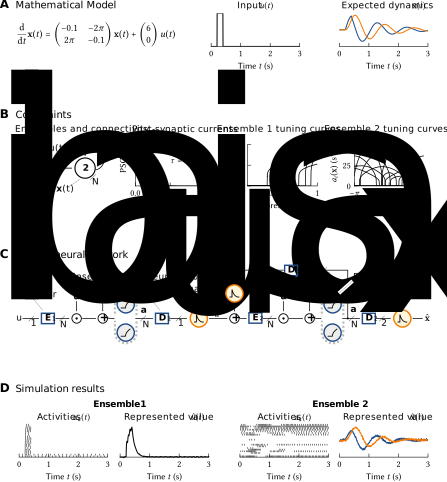
\includegraphics{media/chapter_modelling_neurobiological_systems/nef_overview.pdf}
	\caption[Overview of the Neural Engineering Framework]{Overview of the Neural Engineering Framework (NEF).
	\textbf{(A,~B)} Researchers provide a mathematical model, as well as a set of constraints.
	In this example, constraints are the overall connectivity, tuning properties and filter properties of post-synaptic currents. $\angle \vec x$ denotes the angle of $\vec x = (x_1, x_2)$, i.e., $\angle \vec x = \mathrm{arctan2}(x_2, x_1)$. \textbf{(C)} The NEF can be used to systematically construct a spiking neural network from the given data. This network optimally implements the mathematical model under the given constraints.
	\textbf{(D)} Simulating the network gives insights into how well the mathematical description can be implemented on a neural substrate.
	Spike raster plots with neural activity depict output spikes (short vertical lines) for each neuron (corresponding to rows) over time.}
	\label{fig:nef_overview}
\end{figure}

As we mentioned at the beginning of this chapter, the Neural Engineering Framework\index{Neural Engineering Framework} (NEF; \cite{eliasmith2003neural}) is a modelling framework for neurobiological systems.
The NEF combines techniques from engineering and mathematics---particularly control and dynamical systems theory---with the neurobiological concepts discussed before.
The goal is to allow researchers to map high-level descriptions of cognitive phenomena onto low-level, idealised spiking neural networks.
As such, the NEF provides a synthesis of bottom-up and top-down modelling, and is an attempt at a theory of neuroscience that spans multiple levels of analysis.

To use the NEF, researchers systematically apply three \enquote{principles} that encapsulate key assumptions about neurobiological systems.
These principles exploit neural nonlinearities and synaptic filters to describe how vectorial quantities can be represented, transformed, and made to follow certain dynamics in a spiking neural computational fabric.
The resulting neural networks adhere to mechanistic constraints, such as neural connectivity, maximum firing rates, tuning properties, and synaptic time-constants.
This is illustrated schematically in \Cref{fig:nef_overview}.
A software tool that automates the process of translating mathematical models into spiking neural networks using the NEF principles is part of the Nengo\index{Nengo} spiking neural network simulator package \citep{bekolay2014nengo}.\footnote{See \url{https://www.nengo.ai/} for more information on Nengo. Nengo is free for non-commercial use.}


%\begin{enumerate}[1.]
%	\item \emph{Representation.}
%	The momentary activity $\vec a \in \mathbb{R}^{\Npop}$ of an ensemble of \Npop neurons represents a vectorial quantity $\vec x \in \mathbb{R}^d$. The encoding process mapping $\vec x$ onto activities $\vec a$ is nonlinear,
%	the decoding process is linear.
%	That is, there exists a matrix $\Dec \in \mathbb{R}^{d \times \Npop}$ such that $\vec x \approx \vec \Dec \vec a(\vec x)$.
%	\item \emph{Transformation.}
%	Synaptic connections between neural ensembles approximate non-linear transformations $f(\vec x)$ applied to the represented values, where $f : \mathbb{R}^d \longrightarrow \mathbb{R}^{d'}$ and $d$ and $d'$ are the dimensionalities of the quantities represented in the individual ensembles.
%	\item \emph{Dynamics.}
%	Represented values are state variables $\vec x(t)$ in a dynamical system. Recurrent connections approximate arbitrary dynamical systems of the form $\dot{\vec x} = f(\vec x(t), \vec u(t), t)$.
%	Here, $\vec x(t)$ is the represented value, $\vec u(t)$ is some external input, and $t$ is the current time.
%\end{enumerate}

In this section, we first discuss applications of the NEF from the perspective of the cognitive sciences (model validation and hypothesis generation), as well as engineering and computer science (a programming model for neuromorphics).
We continue with a detailed description of the theory underpinning the NEF, and conclude with a list of limitations that we address in the next chapters.

% TODO: References to other frameworks!!!!

\subsection{Model Validation and Hypothesis Generation}

As we alluded to in the introduction of this chapter, models built using the NEF bridge multiple levels of analysis.
That is, they implement high-level behaviour (given as a mathematical description) using low-level mechanisms (spiking neurons and synapses).
This facilitates model validation and hypothesis generation.

\subsubsection{Model validation}
The concept of model validation generally refers to comparing a model to empirical measurements \citep{adams2012assessing}.
In the case of NEF models, we can, of course, compare the high-level behaviour of the biological system to that of the constrained network model.
The smaller the deviations, the \enquote{better} the original mathematical model.%
\footnote{Of course, naively evaluating models in this manner does not account for overfitting. The model could inadvertently be tuned to reproduce the behaviour of interest, but not be able to generalise to different scenarios. In contrast to other machine learning approaches, overfitting in this sense is typically less of a problem with NEF models.
This is due to the transparency of the training process, only few (typically hand-selected) parameters, and biological constraints, all of which can be seen as regularisation.}
While such comparisons would also be possible with the high-level model alone, biological constraints can drastically influence the high-level behaviour of the model---hence, the NEF is a good litmus test for the suitability of a mathematical model to be realized on a neural substrate.
This is because the NEF \emph{optimally} implements a set of mathematical equations as an idealized spiking neural network.
If the model cannot be realized on a spiking neural substrate despite these idealised conditions, it is unlikely that it describes a biological process well.

NEF models can also be compared in terms of detailed neurophysiological data, and not just high-level behaviour.
Because NEF models are based on a biologically plausible neural substrate, researchers can measure neurophysiological quantities, such as spike trains, local field potentials, or blood oxy\-gen\-ation \citep[Chapters 5.8~\&~9.4]{eliasmith2013how}.
Examples of this can be found in \citet{stewart2012learning,bekolay2014spiking,duggins2017effects,voelker2018improving,gosmann2021cue}.

\subsubsection{Hypothesis generation}
There are two ways in which the NEF aids \emph{hypothesis generation}.
First, and closely related to model validation, deviations between the constrained simulation and the original mathematical model may indicate that the high-level description cannot be realised by the biological system.
Hence, the NEF can be used to reject unsuitable hypotheses and to guide theories towards higher degrees of biological plausibility.
Examples of cognitive theories developed in conjunction with the NEF include the Semantic Pointer Architecture (SPA; \cite{eliasmith2013how}) and SPAUN (the \enquote{Semantic Pointer Architecture Unified Network}), a functional brain model capable of a variety of cognitive tasks \citep{eliasmith2012largescale}.

Second, NEF models can be used to predict the behaviour of a system in experimental paradigms for which no empirical data exists (yet).
This prediction then forms a hypothesis that can be compared to future empirical data.
Furthermore, the NEF also enables the systematic variation of observed biological parameters (e.g., time constants or connectivity), which is often not easily possible in real biological systems.
Assessing the system performance in such artificial situations may yield hypotheses as for why evolution favoured certain parameter combinations.
We give an example of this in Chapter~5.
%TODO: Chapter 5 reference

\subsection{Applications to Neuromorphic Computing}

The scientific applications discussed above were the primary motivation for the development of the NEF \citep[Chapter~1]{eliasmith2003neural}.
However, coincidentally, the same methods are useful as a programming model for neuromorphic computers \citep{boahen2017neuromorph}.

\subsubsection{Neuromorphic computers}
This term\index{neuromorphic computer} refers to computer systems that---to some degree---mimic information processing in the brain.
This typically implies numerous simple computational units, \emph{neurons}, connected via a flexible interconnect \citep{furber2016largescale}.
Beyond these basic characteristics there is no consensus as for what exactly constitutes a \enquote{neuromorphic computer}.
However, most neuromorphic hardware systems execute computations asynchronously and possess provisions for sparse event-based signalling.
Akin to biology, individual computational units independently generate binary events.
In contrast to artificial neural networks, computation is inherently temporal; communication only occurs sporadically and does not carry continuous values.
Hence, the underlying communication infrastructure is solely responsible for signalling spike events, minimising the amount of data that needs to be transferred.

Current neuromorphic computers can be roughly split into two categories, depending on the specific realisation of the computing elements.
Computation either takes place in analogue model circuits, similar to the LIF circuit discussed above, or digital processors with varying degrees of programmability.
% TODO: Add reference to the LIF circuit
Examples of systems in the former \enquote{mixed-signal}\index{neuromorphic computer!mixed signal} category include Braindrop\index{Braindrop} \citep{neckar2019braindrop} and BrainScaleS\index{BrainScaleS} \citep{schemmel2010waferscale}.
Systems that fall into the latter \enquote{purely digital}\index{neuromorphic computer!digital} category are SpiNNaker\index{SpiNNaker} \citep{furber2013overview} and Loihi\index{Loihi} \citep{davies2018loihi}. See \citet{furber2016largescale} for a more comprehensive, albeit slightly outdated list.

\subsubsection{Applications of neuromorphic computing}
The primary motivation behind neuromorphic hardware is to construct computing hardware that approaches the energy efficiency of biological brains \citep{boahen2017neuromorph}.
Compared to conventional computer architectures, these energy savings are mostly due to the asynchronous nature of the computational units, as well as the reduction in communication bandwidth due to event-based signalling \citep{painkras2013spinnaker}.
Furthermore, mixed-signal neuromorphic computers with analogue model circuits benefit from each computational unit operating close to the theoretically required minimum energy \citep{boahen2017neuromorph}.
However, compared to purely digital systems, such analogue designs are much more challenging from an engineering perspective.

Being able to reliably simulate large spiking neural networks with a low energy footprint would be a major scientific breakthrough.
For example, this would enable large-scale brain simulations that are infeasible with conventional supercomputers \citep{calimera2013human}.
From an engineering perspective, being able to map artificial neural networks onto neuromorphic computers could greatly reduce energy costs of machine learning in the data centre and enable new mobile applications of artificial intelligence \citep{hunsberger2016training,blouw2018benchmarking,goltz2020fast,blouw2020eventdriven}.
% TODO: Cite NMI paper instead of goltz2020fast once it has been published
Due to the inherent temporal aspect of the computation, spiking neural networks and neuromorphic hardware are particularly well suited for applications requiring real-time stream processing, such as robotic control or autonomous drones \citep{komer2015biologically,yan2021comparing}.

\subsubsection{The NEF as a programming model for neuromorphic computers}
While, as of writing, several neuromorphic hardware platforms are available to the wider research community, a remaining challenge is to actually program these systems.
Since the computational fabric of neuromorphic computers is similar to biological neural substrates, the NEF can be used to translate mathematical descriptions of dynamical systems into network models that can be executed on the hardware system \citep{boahen2017neuromorph}.
The given constraints can be used to reflect the capabilities of the hardware and to specify the desired precision of the computation.
A variety of neuromorphic platforms have been included as an execution target in Nengo, catering to both scientific and engineering applications.

\pagebreak

\subsection{Principle 1: Representation}

\label{sec:nef_representation}

As we saw above, the Neural Engineering Framework has useful applications in both science and engineering.
In the first part of this thesis, we discuss extensions to the NEF that allow us to model neurobiological circuits more accurately and take better advantage of the computational resources found on neuromorphic computers.
In preparation for these extensions, we now provide a detailed discussion of the aforementioned \enquote{three principles} at the core of the NEF.

The first two NEF principles are best explained assuming steady-state average activities, although, as mentioned before, biological neural networks inherently form dynamical systems.
However, our use of average rate approximations should not be interpreted as the adoption of a \enquote{rate code} by the NEF, but, as we discuss below, is a convenience for solving the synaptic weight optimization problem.
All optimisations can be done in the spiking domain, but the computational costs are significantly higher~\citep{macneil2011finetuning}.

For now, our goal is to map static equations of the form $\vec y = f(\vec x)$ onto rate approximations of spiking neural networks.
The first NEF principles describes how neural populations to represent quantities such as $\vec x$ and $\vec y$.
Paraphrasing \citet{eliasmith2003neural}:
\begin{framed}
\noindent\emph{NEF Principle 1.}
The momentary activity $\vec a \in \mathbb{R}^{\Npop}$ of a population of \Npop neurons represents a vectorial quantity $\vec x \in \mathbb{R}^d$. The encoding process mapping $\vec x$ onto activities $\vec a$ is nonlinear,	the decoding process is linear.
That is, there exists a matrix $\Dec \in \mathbb{R}^{d \times \Npop}$ such that $\vec x \approx \vec \Dec \vec a(\vec x)$.
\end{framed}
There are two fundamental assumptions in this principle that deserve to be untangled.
First, we assume that neuron \emph{populations} form basic functional units and, second, that biological systems represent vectorial quantities.
We already discussed the first assumption regarding populations in more detail in \Cref{sec:neural_tuning}.
To summarise, neighbouring neurons are sensitive to the same quantity and neural activities are noisy---this suggests that nervous systems use population codes.
The second assumption deserves more explanation, given that vectors are abstract mathematical objects.

\subsubsection{Vectorial representations}
The assumption that populations represent vectors $\vec x \in \mathbb{R}^d$ is---to some degree---a mathematical convenience.
Many mathematical objects have useful equivalent vectorial representations, including functions \citep[Chapter 3]{eliasmith2003neural}, probability densities \citep[Chapter 9]{eliasmith2003neural}, and symbols (via vector symbolic architectures; see \cite{gayler2003vector}, \cite{eliasmith2012largescale} and \cite{eliasmith2013how}).
% TODO: Reference review of function spaces

Additionally, there is strong evidence that the activities of neural populations form smooth low-dimensional manifolds\index{manifold} in a high-dimensional activity space \citep{gallego2017neural,stringer2019highdimensional}.
There exists a mapping $\vec a: \mathbb{R}^d \longrightarrow \mathbb{R}^{\Npop}$ (with $d \ll \Npop$) between a low-dimensional vector $\vec x \in \mathbb{R}^d$ and the average neural activities $\vec a(\vec x) \in \mathbb{R}^{\Npop}$, where \Npop is the number of neurons in the population.
If the population exhibits activities $\vec a(\vec x)$ associated with a value $\vec x$, then the population \emph{represents} a \Ndim-dimensional quantity $\vec x$.

\subsubsection{Encoding vectorial quantities}

\begin{figure}
	\centering
	\includegraphics{media/chapter_modelling_neurobiological_systems/nef_representation_2d.pdf}
	{\phantomsubcaption\label{fig:nef_representation_2d_surface}}
	{\phantomsubcaption\label{fig:nef_representation_2d_unit_circle}}
	\caption[Obtaining bell-shaped tuning curves when using two-dimensional encoders]{Obtaining bell-shaped tuning curves when using two-dimensional encoders. Figure adapted from \citet[Figure~2.8, p.~52]{eliasmith2003neural}.
	\textbf{(A)} Surface plot of the tuning curve of a single neuron. Orange arrow is the encoder $\vec e_i$.
	\textbf{(B)} Tuning curve for a represented value $\vec x$ of constant magnitude over the angle $\angle \vec x$.
	Orange triangle corresponds to the direction of the encoding vector.
	The neuron is most active for represented values pointing in this direction.
	}
	\label{fig:nef_representation_2d}
\end{figure}

As we have discussed in \Cref{sec:neural_tuning}, the relationship between a stimulus $\vec x$ and activities of an individual neuron are also referred to as a \enquote{tuning curve}.
While tuning curves in neuroscience are typically defined over scalar quantities, \citeauthor{eliasmith2003neural} propose a parametrised encoding equation $a_i(\vec x)$ that maps $\vec x \in \mathbb{R}^{\Ndim}$ onto the activities of the $i$th neuron in a population---similar to the mathematical model we presented to describe tuning curves in the Hubel and Wiesel experiment (\Cref{sec:neural_tuning},  \Cref{fig:visual_cortex_receptive_field_example} and eq.~\ref{eqn:tuning_curve_from_receptive_field}):
\begin{align}
a_i(\vec x) = G\big[J_i\big(\langle \vec x, \vec e_i \rangle\big)\big] = G\big[\alpha_i\langle \vec x, \vec e_i \rangle + \beta_i\big] \,,
 \quad\quad \text{where } i \in \{1, \ldots, N\} \,.\label{eqn:encoding}
\end{align}
Depending on the interpretation, the encoding vector $\vec e_i$ is equivalent to the \enquote{receptive field} or \enquote{preferred direction} of the neuron.
For example, as depicted in \Cref{fig:nef_representation_2d}, a two-dimensional encoding vector can be used to construct bell-shaped tuning curves similar to those discussed in the context of orientation tuning in the visual cortex; here, the vector $\vec e_i$ would stand for a preferred direction.
Of course, $\vec e_i$ and $\vec x$ could also be discretised visual stimuli---in this case, $\vec e_i$ would be a receptive field and \cref{eqn:encoding} is a direct approximation of \cref{eqn:tuning_curve_from_receptive_field}.

The response curve $G[J]$ depends on the underlying neuron model; for example, we derived the response curve for LIF neurons in \Cref{sec:simplified_neuron_models} (eq.~\ref{eqn:lif_response_curve}); 
the current translation function $J_i(\xi)$ is typically an affine mapping parametrised by a gain $\alpha_i$ and a bias current $\beta_i$.

When building NEF systems, modellers chose the parameters of $a_i(\vec x)$ to characterise how a stimulus $\vec x$ \emph{should} be reflected in the activities of individual neurons.
This last emphasis on \emph{should} is important.
Modellers establish a \emph{normative constraint}.
They specify what the desired tuning should \emph{optimally} be---for example, taking biological data into account.
The purpose of the NEF is to ensure that this constraint is met in a network context.


\begin{figure}
	\centering
	\hspace{-0.2cm}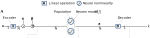
\includegraphics{media/chapter_modelling_neurobiological_systems/nef_representation_diagram.pdf}
	\includegraphics{media/chapter_modelling_neurobiological_systems/nef_representation.pdf}
	{\phantomsubcaption\label{fig:nef_representation_diagram}}
	{\phantomsubcaption\label{fig:nef_representation_current_translation}}
	{\phantomsubcaption\label{fig:nef_representation_tuning_curves}}
	{\phantomsubcaption\label{fig:nef_representation_deocding}}
	\caption[Representation in the Neural Engineering Framework]{Representation in the Neural Engineering Framework. Example for a population of $N = 10$ neurons representing a one-dimensional quantity.
	\textbf{(A)} Schematic overview of the encoding and decoding process.
	\textbf{(A)} Randomly selected affine current translation functions $J_i(\xi) = \alpha_i \langle \vec x, \vec e_i \rangle + J^\mathrm{bias}_i$. The dotted line corresponds to the activity threshold $J_\mathrm{th}$.
	\textbf{(B)} Tuning curves for each neuron in the population after applying the somatic nonlinearity $G[J]$~(eq.~\ref{eqn:lif_response_curve}).
	\textbf{(C)} Reconstructing the represented value from neuron activity by means of linear decoding. Dashed line corresponds to the }
	\label{fig:nef_representation}
\end{figure}

\subsubsection{Selecting encoders, gains, and biases}
Of course, this raises the question of how modellers should select encoders $\vec e_i$, biases $\beta_i$, and gains $\alpha_i$.
To form a good basis for a population code, the population must exhibit diverse tuning (cf.~\Cref{fig:population_code}).
At the same time, the tuning curves must stay within modelling constraints such as the maximally observed firing rates $a_i$ for the range of stimuli $\vec x$ over which we characterise the neuron population.
We denote the set of represented values as a compact set \Xrepr with finite, non-zero volume $\vol(\Xrepr)$.

Unless more specific data are available, we can for example assume that $\vec x$ are within a hyperball of radius $r$, i.e., $\Xrepr = r \Ball^d$.
The encoding vectors $\vec e_i$ can be sampled from the unit hypersphere $\mathbb{S}^d$.
For monotone increasing response curves $G$, gain $\alpha$ and bias $\beta$ can be computed for each neuron by sampling an \enquote{$x$-intercept}\index{x-intercept} value $\xi_0$ from the interval $[-r, r]$ and a maximum rate $a_\mathrm{max}$ and to solve for $\alpha$, $\beta$ such that the following equations hold:
\begin{align*}
	\alpha \xi_0 + \beta &= J_0 = G^{-1}[0] \,, &
	\alpha r + \beta &= J_\mathrm{max} = G^{-1}[a_\mathrm{max}] \,, & \text{where } G^{-1}[a] &\coloneqq \max \big\{ J \mid G[J] = a \big\} \,.
\end{align*}
We get $(r - \xi_0) \alpha = J_\mathrm{max} - J_0$, $(r - \xi_0) \beta = (r J_0 - \xi_0 J_\mathrm{max})$.
For example, for each tuning curve in \Cref{fig:nef_representation}, we randomly sampled a $\xi_0$ from a uniform distribution over $[-1, 1]$, and a maximum firing $a_\mathrm{max}$ rate uniformly from $[10, 50]$.

\subsubsection{Computing identity decoders}
\Cref{eqn:encoding} describes the average neural activities $\vec a$ we expect when a population is representing a certain value $\vec x$; that is, this equation describes how quantities $\vec x$ are \emph{encoded} in a neural network.
Complementary to encoding is \emph{decoding}.
That is, given the activities $\vec a$, we would like to reconstruct the represented $\vec x$.
This could---for example---be accomplished using Bayesian inference, as we demonstrated in \Cref{fig:population_code}.
If the number of neurons \Npop in a population is large enough we can, to a very similar effect, just use a linear decoding matrix \Dec (\Cref{fig:nef_representation}).

The idea is to simply multiply the activities $\vec a$ with a matrix $\Dec \in \mathbb{R}^{d \times \Npop}$ such that the decoded $\vec{\hat x} = \Dec \vec a(\vec x)$ is approximately equal to the encoded $\vec x$, for any $\vec x \in \Xrepr$.
Under the assumption that the activities $\vec a$ are subject to independent and identically distributed (i.i.d.) zero-mean Gaussian noise with standard-deviation $\sigma$, the decoding matrix \Dec can be obtained by minimizing a least-squares loss-function $E$:
\begin{align}
	E &= \frac{1}{\vol(\Xrepr)} \iint_{\Xrepr} \bigl\| \vec x - \Dec \bigl( \vec a(\vec x) + \nu \bigr) \bigr\|_2^2  \, \mathrm{d}\vec{x} \quad\quad \text{where } \nu \sim \Normal(0, \sigma) \,.
	\label{eqn:lstsq_loss_identity}
\end{align}
Of course, minimizing this integral directly is infeasible.
We approximate a solution numerically by drawing \Nsmpls samples from \Xrepr, denoted $\vec x_1$, $\ldots$, $\vec x_N$.
Arranging the samples and the corresponding population activities in matrices $\mat X = \begin{pmatrix} \vec x_1, \ldots, \vec x_{\Nsmpls} \end{pmatrix} \in \mathbb{R}^{\Nsmpls \times \Ndim}$ and $\mat A = \begin{pmatrix}\vec a(\vec x_1), \ldots, \vec a(\vec x_{\Nsmpls})\end{pmatrix} \in \mathbb{R}^{\Nsmpls \times \Npop}$, we can phrase finding \Dec as a Tikhonov regularised least-squares optimization problem
\begin{align}
\min_{\Dec} \sum_{k = 1}^{\Nsmpls} \| \Dec \vec a(\vec x_k) - \vec x_k \|_2^2  + \| \sigma \Dec \|^2_\mathrm{F}
&= \min_{\Dec} \| \mat A \Dec^T - \mat X \|_\mathrm{F}^2 + \sigma^2 \Nsmpls \| \Dec \|_\mathrm{F}^2 \,,
\end{align}
where $\lambda = N \sigma^2$ is the regularisation factor.
From a probabilistic perspective, this particular choice of $\lambda$ results in the exact maximum a-posteriori solution for $\mat D$ with the prior assumption that there is Gaussian noise with standard deviation $\sigma$ on the measurements $\mat A$ \citep[Chapter~6]{boyd2004convex}. 
Larger $\lambda$ increase the robustness of the solution with respect to noise, but decrease the noise-free approximation error.
The solution can be expressed in terms of the regularised Moore-Penrose pseudo-inverse (cf.~Appendix~A.2):
\begin{align}
\Dec^T &= \mat A^+ \mat X \,, &\text{where} \quad \mat A^+ &= \bigl(\mat A^T \mat A + \lambda N \mat I \bigr)^{-1} \mat A^T \,.
\label{eqn:decoding}
\end{align}
As explored by \citet[Chapter~2]{eliasmith2003neural}, the decoding error $E$ tends to decrease with $\mathcal{O}(\sqrt{n})$, assuming that the tuning curves have uniform $x$-intercepts and random encoders $\vec e_i$.
An example of this decoding scheme is given in \Cref{fig:nef_representation_deocding}.

Note that, as mentioned before, we do not take dynamics into account when computing the decoders \Dec.
However, as we discuss next, the same \Dec can be used to decode represented values through time in spiking networks when defining activity $\vec a(t)$ as low-pass filtered population spike trains.
We explicitly take temporal aspects of neural computation into account in \Cref{sec:nef_dynamics} below, and when we discuss temporal tuning in Chapter~4.

\pagebreak

\subsection{Principle 2: Transformation}
\label{sec:nef_transformation}

The representation principle maps vectors $\vec x$ onto average neural activities $\vec a(\vec x)$.
Of course, individual neuron populations seldom exist in isolation.
To construct \emph{networks} that realise the desired tuning properties, we need to determine synaptic weights $w_{ij}$ that describe the connection strength between the $j$th pre- and the $i$th post-neuron.
In addition to realising the chosen representations, the NEF puts a further modelling constraint on the synaptic weights:
\begin{framed}
\noindent\emph{NEF Principle 2.} Synaptic connections between neural ensembles approximate non-linear transformations $\vec y = f(\vec x)$, where $\vec x \in \mathbb{R}^d$ is the value represented in the pre-population, and $\vec y \in \mathbb{R}^{d'}$ the value represented in the post-population.
\end{framed}

\begin{figure}
	\centering
	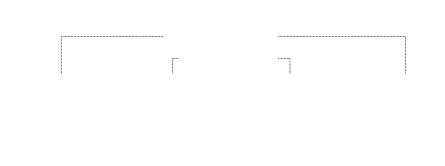
\includegraphics{media/chapter_modelling_neurobiological_systems/nef_transformation_annotations.pdf}%
	\kern-157.19mm\includegraphics{media/chapter_modelling_neurobiological_systems/nef_transformation.pdf}
	\caption[Examples of the function decoding scheme.]{Examples of the function decoding scheme. Instead of decoding the represented value $\vec x$ from a neuron population, we can approximate arbitrary functions $f(\vec x)$.
	\textbf{(A)} $\Npop = 20$ tuning curves $\vec a(x)$; same parameters as in \cref{sec:nef_representation}. \textbf{(B-E)} Different linear decodings $\mat D^f \vec a(x)$ of the above tuning curves. Dotted line is the target function, thick line the decoded function. Inset $E$ is the RMSE.
	}
	\label{fig:nef_transformation}
\end{figure}

That is, modellers can choose a transformation $f$ that should be computed in a connection.
We can easily approximate functions $f$ of the value $\vec x$ represented in a pre-population using a \emph{function decoder} $\Dec^f$.
This $\Dec^f$ has the property that $\vec{\hat y} = \Dec^f \vec a(\vec x)$ is approximately equal to $f(\vec x)$.
Modifying the least-squares loss from \cref{eqn:lstsq_loss_identity}, we get
\begin{align}
	E &= \frac{1}{\vol(\Xrepr)} \iint_{\Xrepr} \bigl\| f(\vec x) - \Dec \bigl( \vec a(\vec x) + \nu \bigr) \bigr\|_2^2  \, \mathrm{d}\vec{x} \quad\quad \text{where } \nu \sim \Normal(0, \sigma) \,.
	\label{eqn:lstsq_loss_f}
\end{align}
Analogously to above, a discrete approximation of $\mat D^f$ for \Nsmpls samples ${\vec x}_1$, $\ldots$, ${\vec x}_{\Nsmpls}$ is given as 
\begin{align*}
	\bigl(\Dec^f\bigr)^T &= \mat A^+ \mat Y \,, &\text{where } \mat A &= \begin{pmatrix}\vec a(\vec x_1), \ldots, \vec a(\vec x_{\Nsmpls})\end{pmatrix} \in \mathbb{R}^{\Nsmpls \times \Npop} \,, & \mat Y &= \begin{pmatrix}f(\vec x_1), \ldots, f(\vec x_{\Nsmpls})\end{pmatrix} \in \mathbb{R}^{\Nsmpls \times \Ndim'} \,.
\end{align*}
Examples of functions decoded from $\vec a(\vec x)$ are depicted in \Cref{fig:nef_transformation}.
The decoding error $E$ depends on the number of pre-neurons \Npop, as well as the \enquote{smoothness} of the decoded function.

\begin{figure}
	\centering
	\vspace{0.25mm}
	\includegraphics{media/chapter_modelling_neurobiological_systems/nef_transformation_diagram.pdf}
	\caption[Neuron populations in the NEF as a single hidden-layer artificial neural network]{Neuron populations in the NEF form a single hidden-layer artificial neural network. Encoders $\mat E$, gains $\vec \alpha$, and gains $\vec \beta$ correspond to a fixed input transformation. The function decoder $\Dec^f$ forms a set of linear output weights. Since the input transformations are fixed, computing $\Dec^f$ is simple.}
	\label{fig:nef_transformation_diagram}
\end{figure}

\subsubsection{Comparison to artificial neural networks}
From the perspective of artificial neural networks, the NEF characterises neuron populations as a single-hidden layer neural network with a fixed input transformation consisting of the encoders, gains, and biases.
Since the input transformation up to the neural nonlinearity---approximated by the response curve $G[J]$---is fixed, learning the output weights---the function decoder---is a convex optimisation problem and no stochastic optimisation such as gradient descent is required (\Cref{fig:nef_transformation_diagram}).

Similar nonlinear encoding and linear decoding schemes have been explored in machine learning for decades.
One early example are the radial basis function networks described by \citet{broomhead1988radial}.
Going back even further, the overall idea is similar to the pattern-recognition model of granule cell activity in the cerebellum proposed by \citet{marr1969theory}.
From a more theoretical perspective, neuron population tuning-curves $\vec a(\vec x)$ span a function space with a set of non-orthogonal basis functions. 
\citet{hornik1989multilayer} show that---assuming a reasonable distribution of these basis functions---we can approximate any continuous function over \Xrepr to a desired degree by increasing the number of hidden units.
% TODO: Reference to other basis function related stuff

\subsubsection{Computing synaptic weights}
As we have seen, function decoders $\Dec^f$ can approximate arbitrary functions $f$ over \Xrepr.
Of course, this is only half of what we set out to accomplish.
Our goal was to find synaptic weights $\mat W \in \mathbb{R}^{m \times n}$ that connect from a pre-population of \Npop neurons representing $\vec x$ to a post-population of $m$ neurons, such that the tuning properties of the target population are preserved, \emph{and} the post-population is representing a transformed version $f(\vec x)$.

If we assume that the current translation function $J_i(x)$ is an intrinsic part of each post-neuron $i$, encoding and decoding can be linearly combined into a weight vector $\vec w_i$:
\begin{align}
	a_i^\mathrm{post}\bigl(f(\vec x)\bigr)
		&\approx
	a_i^\mathrm{post}\bigl(\mat D^f \vec a_\mathrm{pre}(\vec x)\bigr)
		=	
	G\bigl[J_i\bigl(\langle \vec e_i^T, \mat D^f \vec a^\mathrm{pre}(\vec x)\rangle \bigr)\bigr]
		=
	G\bigl[J_i\bigl(\langle \vec w_i, \vec a^\mathrm{pre}(\vec x) \rangle \bigr)\bigr] \,.
	\label{eqn:nef_weight_vector}
\end{align}
Hence, $\mat W = \mat E \mat D^f$ forms a synaptic weight matrix, where $\mat E \in \mathbb{R}^{m \times d'}$ is a matrix of post-population encoding vectors $\vec e_i$, and $\mat D^f$ is the pre-population function decoder.
This matrix implicitly decodes $\vec{\hat y} = f(\vec x)$ from a pre-population, and re-encodes $\vec{\hat y}$ in the post-population.

%Note that these synaptic weights directly translate the pre-population activities into an average current that is injected into the post-neuron.
%Although biological neural networks do not possess \enquote{encoding} and \enquote{decoding} matrices with intermediate low-dimensional representations, the product $\mat W = \mat E \Dec^f$ has the equivalent effect of first decoding, and then re-encoding.

A welcome side-effect of this formalisation is that the weight matrix $\mat W$ is of low rank.
This significantly reduces the amount of computation required to evaluate NEF networks.
Consider a matrix-vector product of the form $\mat W \vec a$.
Evaluating this requires $\mathcal{O}(mn)$ operations, where \Npop and $m$ are the number of neurons in the pre- and post-population.
In contrast, multiplying the low-rank factorisation with an activity vector, i.e., computing $\mat E ( \mat D \vec a 
)$, requires only $\mathcal{O}(\Ndim n + \Ndim' m)$ operations.
Since, typically, $d \ll n$ and $d' \ll m$, this is a linear time operation.
Along with the linearity of homogeneous synaptic filters, this is what enables Nengo to simulate large spiking neural networks on commodity hardware \citep{bekolay2014nengo}.

\subsection{Principle 3: Dynamics}
\label{sec:nef_dynamics}

% TODO: Mention the key-word recurrent somwhere!

\begin{figure}
	\centering
	\includegraphics{media/chapter_modelling_neurobiological_systems/instantaneous_spike_rate.pdf}%
	{\phantomsubcaption\label{fig:instantaneous_spike_rate_a}}%
	{\phantomsubcaption\label{fig:first_order_low_pass}}%
	\caption[Estimating the instantaneous firing rate using a synaptic filter]{Estimating the instantaneous firing rate using a first-order exponential synaptic filter. \textbf{(A)} Blue line depicts a spike train (short black lines at the bottom) filtered by a first-order exponential low-pass filter $h(t)$ with $\tau = \SI{0.1}{\second}$. The black line is the \enquote{ground-trouth} rate underlying the spike train (using a $\Delta\Sigma$-modulator).
	Apart from a phase shift and some added noise, the low-pass filtered spike train tracks the ground truth well.
	\textbf{(B)} Visualisation of the synaptic filter $h(t)$. We assume that spikes are Dirac deltas and that the filter has unit DC-gain, i.e., the area under the curve is one.}
	\label{fig:instantaneous_spike_rate}
\end{figure}

So far, and as mentioned several times before, we have ignored the fact that spiking neural networks possess temporal dynamics.
Instead, and very similar to the rate-based artificial neural networks used in machine learning, we assumed average firing rates in the encoding and decoding equations.
Fortunately, this is less of a problem as it may seem.

Synaptic dynamics (cf.~\Cref{sec:synaptic_transmission}) act as a filter that estimates the pre-synaptic \emph{instantaneous firing rate} of a spike train.
The instantaneous firing rate is the spike rate $a_i$ of a neuron at a single point in time $t$.
Of course, this is a quite paradoxical notion.
As mentioned before, by the Fourier uncertainty principle\index{Fourier uncertainty principle}, we cannot measure an event rate without averaging over time; the smaller the time-window, the smaller the frequency resolution (cf.~\cite{gabor1946theory}).

Still, low-pass filters can be reasonably effective to infer the state of a process generating binary events.
This is illustrated in \Cref{fig:instantaneous_spike_rate}.
The low-pass filtered spike train is clearly centred around the ground-truth rate.
The deviations from the ground-truth can be interpreted as noise.
Conveniently, we already accounted for noise by relying on population codes, and regularising the decoding matrices $\mat D^f$ (eq.~\ref{eqn:lstsq_loss_f}).
More information on this topic can be found in \citet[Chapter~4]{eliasmith2003neural}, as well as later in Chapter~4 of this thesis.
%TODO: Reference to Chapter 4.

This discussion should have reassured the reader that the techniques discussed so far will also work in the context of spiking neural networks.
However, a central tenet of the NEF is that we would not just like to translate mathematical descriptions into spiking neural networks that \emph{work}.
Instead, we would also like to know how resources available in biologically plausible spiking neural networks can \emph{support} high-level function.

In this vein, the third NEF principle describes how synaptic filters can be exploited to approximate arbitrary dynamical systems.
Paraphrasing \citet{eliasmith2003neural}:
\begin{framed}
	\noindent\emph{NEF Principle 3.}
	Represented values are state variables $\vec x(t)$ in a dynamical system. Recurrent connections approximate arbitrary dynamical systems of the form $\dot{\vec x}(t) = f(\vec x(t), \vec u(t), t)$, where $\vec x(t)$ is the represented value, $\vec u(t)$ is some external input, and $t$ is the current time.
\end{framed}

\begin{figure}
	\centering
	\includegraphics{media/chapter_modelling_neurobiological_systems/nef_dynamics_diagram_ab.pdf}
	{\phantomsubcaption\label{fig:nef_dynamics_integral}}%
	{\phantomsubcaption\label{fig:nef_dynamics_synaptic}}%
	\caption[Integrator and synaptic filter realisations of an LTI system]{Integrator and synaptic filter realisations of an LTI system. Orange circles depict temporal convolutions.
	\textbf{(A)} The standard LTI system.
	\textbf{(B)} Using a low-pass filter instead of a perfect integrator.}
	\label{fig:nef_dynamics_ab}
\end{figure}

This principle is best explained considering linear time-invariant (LTI) systems of the form
\begin{align*}
	\dot{\vec x}(t) &= \mat A \vec x(t) + \mat B \vec u(t) \,,
\end{align*}
where $\mat A \in \mathbb{R}^{\Ndim \times \Ndim}$ is the feedback matrix, $\mat B \in \mathbb{R}^{\Ndim \times \Ndim'}$ is the input matrix.
Integration yields
\begin{align}
	\vec x(t)
	&=
		\int_0^t \dot{\vec x}(\tau) \,\mathrm{d}\tau + \vec x_0
	=
		\int_0^t \mat A \vec x(\tau) + \mat B \vec u(\tau) \,\mathrm{d}\tau + \vec x_0 \,,
	\label{eqn:lti_integral_equation}
\end{align}
where $\vec x_0$ is the initial state.
Hence, and as illustrated in \Cref{fig:nef_dynamics_integral}, if we have access to an integrator as a computational primitive, we can easily evaluate dynamical systems of this form.
%In practice, such integral equations can be evaluated using some numerical integration method, the simplest (but least powerful) being Euler integration \citep[cf.][Chapter~17]{press2007numerical}.

Unfortunately, biological neural networks do not contain \enquote{perfect} integrators.
Instead, they need to rely on \enquote{leaky} integrators, such as low-pass filters.
It is easy to see why a low-pass filter is a leaky integrator.
The impulse response of an integrator is a step function (i.e., zero for $t < 0$, one for $t \geq 0$).
Similarly, the impulse response $h(t)$ of a first-order low-pass filter jumps to non-zero value at $t = 0$, but in contrast to the integrator, quickly decays (\Cref{fig:first_order_low_pass}).
The key idea of the dynamics principle is to compensate for this \enquote{forgetfulness}.
That is, we change the desired dynamical system to account for leaky integration (\Cref{fig:nef_dynamics_synaptic}).

Despite the name, the \enquote{leaky integrator} dynamics of the LIF neuron itself are of little use.
The neuron resets its state with every output spike, loosing all the integrated information.
Fortunately, the low-pass filter dynamics of synapses are decoupled from the neural superthreshold dynamics.
Moreover, as explained by
\citet[Chapter~8 \& Appendix~F.1]{eliasmith2003neural},
it is not unreasonable to assume that the synaptic filter dominates the overall neural dynamics.
In other words, dynamics mainly stem from the synaptic filter $h(t)$---altough, we revisit this assumption in \Cref{sec:nef_limitations}.

We can easily derive a system that compensates for the low-pass filter dynamics using the Laplace transformation.
Assume that both the feedback and the input passes through the same first-order low-pass filter with time-constant $\tau$.
Treating both the integral in \cref{eqn:lti_integral_equation} and the low-pass filter as convolutions with their respective impulse response, we have
\begin{align}
	X(s) &= \frac{1}{s} \bigl( \mat A X(s) + \mat B U(s) \bigr) & \text{and} \quad\quad X(s) &= \frac{1}{1 + \tau s} \bigl( \mat A' X(s) + \mat B' U(s) \bigr) \,.
	\label{eqn:original_vs_modified_lti}
\end{align}
Rearranging the second equation and comparing coefficients to the first equation we get
\begin{align*}
	X(s) &= \frac{1}{s} \frac{\mat A' - \mat I}{\tau} X(s) + \frac{\mat B'}{\tau} U(s) &
	\leadsto \quad \quad \mat A' &= \tau \mat A + \mat I \,, &
	\mat B' &= \tau \mat B \,.
\end{align*}
For arbitrary dynamics $f(\vec x, \vec u, t)$ we similarly obtain $f'(\vec x, \vec u, t) = \tau f(\vec x, \vec u, t) + \vec x$ \citep[Chapter~8]{eliasmith2003neural}.
In other words, to compensate for low-pass filter dynamics, we scale the dynamics by $\tau$ and feed back $\vec x$ to \enquote{remind} the system of its current state.

\begin{figure}
	\centering
	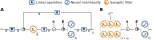
\includegraphics{media/chapter_modelling_neurobiological_systems/nef_dynamics_diagram_c.pdf}%
	{\phantomsubcaption\label{fig:nef_dynamics_neurons_a}}%
	{\phantomsubcaption\label{fig:nef_dynamics_neurons_b}}%
	\caption[Synaptic filters and LTI systems in NEF networks]{Synaptic filters and LTI systems in NEF networks.
	\textbf{(A)} NEF realisation of an LTI system. Homogeneous synaptic filters are modelled as $d$ filters placed before the encoder.
	\textbf{(B)} Technically, each of the $n \times m$ synaptic connections between a pre- and a post-population has its own synaptic filter. When scaled appropriately, the resulting filter matrix replaces the synaptic weights; however, this has drastically higher computational costs than placing $d$ filters ahead of the encoder.}
	\label{fig:nef_dynamics_neurons}
\end{figure}

Using the representation and transformation principles, we can turn the block-diagram in \Cref{fig:nef_dynamics_synaptic} into a spiking neural network.
This is schematically depicted in \Cref{fig:nef_dynamics_neurons_a}.
The decoded state $\vec{\hat x}$ and the input $\vec u$ are passed through compensated LTI matrices $\mat A'$ and $\mat B'$, summed, and fed into the synaptic filters.
We gave an example of this in \Cref{fig:nef_overview}.

Of course, as before, the network can, due to linearity, be expanded into biologically plausible synaptic weights and arrays of synaptic filters (\Cref{fig:nef_dynamics_neurons_b}).
Function decoders $\mat D^f$ can be used to support arbitrary nonlinear dynamics, and not just LTI systems.

\subsection{Some Limitations of the Neural Engineering Framework}
\label{sec:nef_limitations}

To date, the Neural Engineering Framework has seen considerable use in the scientific community (cf.~\Cref{app:nef_literature}).
Nevertheless, the NEF has a series of shortcomings that limit the biological plausibility of the generated networks, the number of constraints exposed to modellers, and how well resources available on some neuromorphic hardware platforms are utilised.
Resolving these issues could make the NEF more appealing to a wider group of researchers and contribute to ongoing efforts in cognitive science and neuromorphic computing.

Of course, the following list of limitations is by no means complete.
To the contrary.
One can quite effortlessly identify areas of neuroscience that are not reflected in the NEF at all---for example nervous system development, or networks of glial cells.
However, as we implied in the beginning this chapter, we think that, as of now, there is too little consensus on these topics to account for them in a general-purpose modelling tool.

Overall, while it is tempting to incorporate as much biological detail as possible into NEF networks, this is misguided if merely done as an end in itself.
Remember that our goal is to bridge low-level mechanism and high-level function.
This distinguishes NEF models from \enquote{bottom-up} approaches, that develop mechanistically detailed models of brain circuits, with the hope that the final system---if truthfully describing biology---exhibits some interesting function \citep[cf.][]{komer2016unified}.
We think that, optimally, extensions to the NEF should expose new low-level detail as a \enquote{computational resource} that can be systematically exploited for high-level function.
At the very least, extensions should expose additional constraints that provide modellers with an opportunity to explore the impact of individual aspects of neurobiological mechanism on high-level function \citep[e.g.,][]{duggins2017incorporating}.
% TODO: Cite Pete's paper when published

%The two main extensions to the NEF we discuss in this thesis---nonlinear dendritic interactions and temporal tuning---fall into the first category, whereas the other extensions provide additional modelling constraints.

\subsubsection{Limitation 1: Current-based synapses}
In our discussion of Principle 2 (\Cref{sec:nef_transformation}), we implicitly assumed that neurons use current-based synapses (cf.~\Cref{sec:simplified_neuron_models}).
As expressed in \cref{eqn:nef_weight_vector}, we model the current injected into the post-neuron as linearly depending on the pre-population activities.
However, as we discussed in \Cref{sec:synaptic_transmission}, synaptic transmission is better modelled in terms of \emph{conductances}, and not currents.
As noted by \citet[Section~2.1.2, p.~35]{eliasmith2003neural}, accounting for conductances adds another layer of nonlinearity to the neuron.
While such nonlinearities have been analysed in the context of the NEF by \citet[Chapter~4]{tripp2009search} as well as \citet{bobier2014unifying}, this prior work does not propose a systematic method for exploiting synaptic nonlinearities for computation.

Adapting the NEF to support nonlinear conductance-based synapses would increase compatibility with neuromorphic hardware platforms emulating conductance-based neurons (e.g.,~BrainScaleS; \cite{schemmel2010waferscale}) and allow modellers to more easily constrain models according to neurophysiological parameters, such as synaptic reversal potentials.
Furthermore, individual synapse types (e.g.,~excitatory and inhibitory) act as independent input channels to a neuron.
As we discuss in the next chapter, these input channels interact non-linearly in the case of multi-compartment neurons, increasing the class of functions that can be approximated using the same number of neurons.


\subsubsection{Limitation 2: Bias currents}
A minor (as we will see) limitation is the assumption that each neuron possess an intrinsic bias current $\beta_i$ (eq.~\ref{eqn:encoding}).
This current is necessary to ensure diverse tuning.
For example, some neurons are active even if no input is present (\enquote{spontaneous} or \enquote{background} activity).
This can be modelled using positive bias currents.

\Citet[Chapter~2; p.~35]{eliasmith2003neural} interpret the bias current as a \enquote{constant input current from the rest of the nervous system}.
While reasonable, this assumption cannot be strictly true.
The mean firing rate of individual populations varies sigificantly over time \citep{okun2012population}; it is not immediately clear how these variations would support constant $\beta_i$.
Hence, an explicit translation of pre-activities into a bias current $\beta_i$ using synaptic connectivity may be preferable.
Depending on the pre-population tuning, this can affect high-level function.


\begin{figure}
	\includegraphics{media/chapter_modelling_neurobiological_systems/granule_jbias_distribution.pdf}%
	{\phantomsubcaption\label{fig:jbias_a}}%
	{\phantomsubcaption\label{fig:jbias_b}}%
	{\phantomsubcaption\label{fig:jbias_c}}%
	{\phantomsubcaption\label{fig:jbias_d}}%
	{\phantomsubcaption\label{fig:jbias_e}}%
	{\phantomsubcaption\label{fig:jbias_f}}
	\caption[Neuron parameter variability only accounts for small bias currents]{Neuron parameter variability only accounts for small bias currents.
	\textbf{(A, B)} Standard NEF tuning curves and corresponding bias current distribution.
	\textbf{(C)} Empirical data on resting potential $v_\mathrm{rest}$ variations in cerebellar granule cells from \citet[Figure~1b]{chadderton2004integration} with a Gaussian fit.
	\textbf{(D)} Noisy LIF neuron response curves for resting potentials samples from the empirical distribution. Colours indicated in \emph{(C)}. Other LIF parameters fit to empirical data at $v_\mathrm{rest} = \SI{-64}{\milli\volt}$ (black crosses; cf.~Figure~1g in Chadderton et al.). Input currents $J$ are subject to Gaussian noise ($\sigma = \SI{10}{\pico\ampere}$). \textbf{(E)} Histogram of bias currents $\beta_i$ having the same average effect as varying $v_\mathrm{rest}$.
	\textbf{(F)}~Tuning curves that can be realised using these bias currents for the target maximum rates.
	}
\end{figure}

Furthermore, and directly related to Limitation~1, pre-synaptic activity affects synaptic \emph{conductances} and does not directly induce \emph{currents}.
This is particularly problematic since tuning curves with uniform $x$-intercepts tend to require large \emph{negative} bias currents (\Cref{fig:jbias_a,fig:jbias_b}).
It is unclear how such currents should be generated, particularly since the inhibitory synaptic reversal potential $E_\mathrm{I}$ is close to the resting potential $v_\mathrm{rest}$.
Natural neuron parameter variations are insufficient to explain this discrepancy (\Cref{fig:jbias_c,fig:jbias_d,fig:jbias_e,fig:jbias_f}).

\begin{figure}
	\includegraphics{media/chapter_modelling_neurobiological_systems/constrained_weight_matrices.pdf}
	{\phantomsubcaption\label{fig:sparsity_and_dales_principle_a}}%
	{\phantomsubcaption\label{fig:sparsity_and_dales_principle_b}}%
	{\phantomsubcaption\label{fig:sparsity_and_dales_principle_c}}%
	\caption[Constrained connectivity and Dale's principle]{Constrained connectivity and Dale's principle. \emph{Top:} Weight matrix $\mat W$ and (if applicable) factorisation into $\mat E, \mat D$. \emph{Bottom:} Weight histogram relative to the $95$-percentile $P_{95}$. Red indicates inhibitory, blue to excitatory weights. \textbf{(A)}~Typical NEF weight matrices are dense.
	\textbf{(B)}~$L_1$-regularisation of decoders $\mat D$ increases sparseness, but does so in an uncontrolled manner. Note that $\mat D$ is (relatively speaking) sparser than $\mat W$.
	\textbf{(C)}~Dale's principle imposes an excitatory/inhibitory split on $\mat W$.
	This is difficult when factorising $\mat W$, but one can solve for $\mat W$ directly using nonnegative least-squares (NNLS).
	}
	\label{fig:sparsity_and_dales_principle}
\end{figure}

\subsubsection{Limitation 3: Constrained connectivity and Dale's principle}
NEF weight matrices $\mat W = \mat E \mat D$ are typically dense.
That is, they contain few zeros, implying all-to-all connectivity between neurons (\Cref{fig:sparsity_and_dales_principle_a}).
However, in biology, connectivity in the brain can be quite sparse.
For example, as detailed by \citet[Chapter~20]{braitenberg1998cortex}, the likelihood of two neighbouring cortical cells to be connected is less than $90\%$. Similarly, connectivity between Golgi and Granule cells in the cerebellum is highly constrained (cf.~Chapter~5).
% TODO: Add reference to Chapter 5
It may be desirable to give modellers the opportunity to account for these statistics.

A common way to enforce sparsity is to use $L_1$, or \enquote{lasso}, regularisation instead of the $L_2$ regularisation proposed in \cref{eqn:lstsq_loss_identity,eqn:lstsq_loss_f} \citep[Chapter~6]{boyd2004convex}.
However, solving for sparse decoders $\mat D$ in this way has two issues.
First, this process is uncontrolled---na\"ive $L_1$ regularisation does not take biological constraints into account.
Second, for $\Ndim \gg 1$, orthogonality between the encoders and decoders determines sparsity, and not just the sparsity of $\mat D$ (\Cref{fig:sparsity_and_dales_principle_b}).
Both issues mandate more complex regularisation terms.

Another form of constrained connectivity is to account for Dale's principle.
As we discussed before in \Cref{sec:synaptic_transmission}, individual neurons typically act either exclusively excitatorily or inhibitorily. Empirical data suggest that, depending on the modeled brain region, excitatory cells outnumber inhibitory cells by a factor between two and four~\citep{hendry1981sizes,gabbott1986quantitative}.
This imposes a certain structure onto the weight matrix (\Cref{fig:sparsity_and_dales_principle_c}).

\begin{figure}
	\centering
	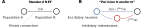
\includegraphics{media/chapter_modelling_neurobiological_systems/parisien_transform.pdf}
	\caption[Illustration of the \enquote{Parisien transform}]{Illustration of the \enquote{Parisien transform}. This transformation accounts for Dale's principle by splitting standard NEF connections, as depicted in \textbf{(A)}, into an excitatory and inhibitory path \textbf{(B)}.}
	\label{fig:parisien_transform}
\end{figure}

\Citet[Section~6.4]{eliasmith2003neural} propose a method to account for Dale's principle later refined by \citet{parisien2008solving}.
The basic idea of this \enquote{Parisien transform} is to decode add a specially crafted \enquote{bias function} to the function computed in excitatory connections originating from the pre-population.
This bias function ensures that all connection weights are positive.
An inhibitory inter-neuron population is then added to the network and connected in parallel to the excitatory connection to subtract the superfluous current induced by the bias function (\Cref{fig:parisien_transform}).

While mathematically clever, the Parisien transform changes the network structure by adding an inhibitory interneuron population.
Although interneurons are indeed common in brain networks, the connectivity patterns resulting from the Parisien transform may not be desirable.
For example, as we discuss in Chapter~5, Golgi cells are recurrent inhibitory interneurons between granule cells.
However, there are no excitatory recurrent connections between granule cells, as assumed by the Parisien transform.
In the next chapter, we discuss a simpler approach to accounting for Dale's principle that is orthogonal to the network structure.

\subsubsection{Limitation~4: Temporal tuning and neural dynamics}
The dynamics principle derived in \Cref{sec:nef_dynamics} was based on two assumptions.
First, synaptic dynamics dominate neural dynamics.
Second, synaptic filters are homogeneous first-order low-pass filters in both the input and recurrent connection.
While reasonable, these modelling assumptions are, as so often, only coarse approximations of biology.

\begin{figure}[t]
	\includegraphics{media/chapter_modelling_neurobiological_systems/firing_rate_neural_dynamics.pdf}
	\caption[Neural dynamics for different maximum firing rates]{Neural dynamics for different maximum firing rates $a_\mathrm{max}$. A \SI{100}{\second} band-limited white-noise signal $u(t)$ with a band-width of \SI{100}{\hertz} is fed through a NEF population with uniform $x$-intercepts.
	The transfer function is determined from the decoded $\hat u(t)$ using the method described in \citet[Section~4.3.3]{eliasmith2003neural}.
	We ensure a constant amount of spike noise by setting the number of neurons in the population to $100\,000 / a_\mathrm{max}$. \emph{Top:} Linear transfer function for different maximum rates $a_\mathrm{max}$. \emph{Bottom:} Slice through the transfer functions at the indicated locations.
	\textbf{(A)} Data for a spiking rectified linear unit (ReLU), a $\Delta\Sigma$-modulator with a rectified input current. This kind of neuron exhibits no significant dynamics of its own, independent of the firing rate. \textbf{(B)} Transfer function for the LIF neuron. For small firing rates, the neuron acts as a low-pass with a relatively moderate attenuation of about \SI{-5}{\deci\bel}. For firing rates of about \SI{200}{\hertz}, the neuron acts as a pass-through. \textbf{(C)} While similar to the LIF neuron, the ALIF
	acts as a very narrow low-pass filter when driven at a maximum firing rate of about \SI{20}{\hertz}. The location of this \enquote{trough} depends on the adaptation time-constant.}
	\label{fig:neural_dynamics_firing_rates}
\end{figure}

The assumption that synaptic dynamics dominate the overall dynamics of a neuron is a good approximation of the behaviour of simple neuron models operating at high firing-rates.
However, for smaller firing rates, the neural dynamics can have a significant impact on the overall system dynamics.
For example, for maximum firing rates below about $\SI{50}{\per\second}$, the sub-threshold low-pass dynamics of the LIF neuron begin to have a moderate effect on the neural dynamics.
This is depicted in \Cref{fig:neural_dynamics_firing_rates}.

While these rate-dependent effects are relatively small, more complex neuron models possess strong internal dynamics.
For example, the adaptive LIF (ALIF) neuron model \citep[Chapter~14]{koch1999biophysics} accounts for firing rate adaptation; that is, each output spike increases the current required to evoke another output spike.
This can be modelled as an inhibitory current resulting from low-pass filtering the neuron's output spike train.
As demonstrated by \citet[Chapter~7]{tripp2009search}, the internal dynamics of the ALIF neuron model can, under certain circumstances, be exploited to implement arbitrary dynamics using a variant of the equations derived for the NEF dynamics principle.

The second assumption, namely that synaptic filters are homogeneous, is likely violated if a neuron possesses multiple receptor types.
As we saw in \Cref{sec:synaptic_transmission}, the synaptic time-constant can vary significantly between (and even within) individual receptor types.
We also saw that synaptic transmission is better modelled by higher-order filters.
\Citet{voelker2018improving} discuss methods to generalise the dynamics principle to arbitrary synaptic filters; however, these methods require explicit higher-dimensional state space representations.

In Chapter~4, we suggest the concept of \enquote{temporal tuning curves} to---at least partially---account for these issues.
Temporal tuning curves are a direct extension of standard NEF tuning curves, and are inspired by the concept of temporal receptive fields.
In essence, we treat both synaptic and neural dynamics as temporal resources that can be harnessed to approximate a desired temporal tuning by solving a simple least-squares problem.
This naturally extends the NEF and unifies the approaches described by Tripp and Voelker in a systematic way.
% Add reference to Chapter~4

	\setcounter{chapter}{2}
	% !TeX spellcheck = en_GB
\chapter{Computational Properties of Multi-Compartment LIF Neurons}

\vspace{30pt}

\begin{OpeningQuote}
It may well be that certain nerve pulse combinations will stimulate a given neuron not simply by virtue of their number but also by virtue of the spatial relations of the synapses to which they arrive. This is, one may have to face situations in which there are, say, hundreds of synapses on a single nerve cell, and the combinations of stimulations on these that are effective [...] are characterised not only by their number, but also by their coverage of certain special regions on that neuron [...], by the spatial relations of such regions to each other, and by even more complicated quantiative and geometrical relationships that might be relevant.
\OpeningQuoteSource{John von Neumann}{The Computer and the Brain (1958)}
\end{OpeningQuote}

\vspace{10pt}

\begin{PriorPublication}
Portions of this chapter (in particular \Cref{sec:two_comp_lif}) are, in extended and heavily edited form, adapted from \citet{stoeckel2021}, which in turn is an extension of work presented at COSYNE 2018 \citep{stockel2018nonlinear}, as well as an earlier technical report \citep{stockel2017point}.
%Chris Eliasmith supervised this work and edited the manuscripts.
%Aaron Voelker contributed with valuable ideas regarding experimental paradigms during the initial research phase.
Whereas these prior publications focus on single- and two-compartment LIF neurons, we deepen the provided theoretical background and define and discuss $n$-LIF neurons in general.
\end{PriorPublication}

\begin{Contributions}
The work in this chapter can be seen as a continuation of the research presented in \citet[Chapter~5]{koch1999biophysics}, as well as \citet[Chapter~4]{tripp2009search}.
In contrast to these prior publication, we discuss a systematic approach to using passive dendritic nonlinearities as a computational resource to approximate arbitrary functions within the context of functional modelling frameworks.
We particularly focus on convex optimisation, ensuring globally optimal solutions.
Additionally, as far as we are aware, the idea to use quadratic programming for subthreshold relaxation is novel.
\end{Contributions}

% !TeX spellcheck = en_GB

% TODO: Add Koch & Softky reference regarding synaptic saturation later in the chapter

As we saw in the previous chapter, neurons possess intricately detailed dendritic trees (cf.~\Cref{fig:neuron_sketches}).
While the growth of these structures can to some degree be modelled by stochastic processes \citep[e.g.,][]{nowakowski1992competitive}, dendrites are not merely a means to establishing random connectivity.
Dendritic development is guided by several extrinsic signals, including the activities of neighbouring neurons \citep{mcallister2000cellular}.
This suggests that dendries are fine-tuned to fulfil a certain computational function.

Indeed, both theoretical and empirical studies imply that the location of synaptic sites within the dendrites has a significant impact on neural computation \citep{mel1994information,koch2002singlecell,polsky2004computational}.
Still, there is no widely accepted high-level theory of dendritic computation \citep{london2005dendritic}, that would, for example, be on a similar level of abstraction as the admirably successful LIF neuron.

Finding such an overarching theory of dendritic computation is difficult due to the sheer complexity of the nonlinear dynamical systems formed by active dendritic structures \citep{beniaguev2021single}.
This may sometimes lead to seemingly contradictory observations.
For example, the distance between a synaptic event and the soma determines the strength of the somatic post-synaptic potential---this is a direct result of the passive cable properties of a neuron (cf.~\Cref{sec:comp}).
In fact, isolated distal spikes hardly influence the somatic membrane potential \citep{stuart1998determinants}.
%\footnote{Interestingly, as explored by \citet{stuart1998determinants}, this attenuation is less of a result of longitudinal resistance, but of leak (or \enquote{resting}) channels being distributed nonuniformly throughout the dendritic cell membrane.}
However, some dendrites with active Hodgkin-Huxley-like cell membranes (cf.~\Cref{sec:neural_dynamics}) negate the effects of distance-dependent attenuation \citep{koch2002singlecell}.
Coincident distal input may trigger dendritic action-potentials that in turn strongly influence the soma \citep{williams2002dependence}.

\subsubsection{Hypothesised dendritic function}
Early theoretical studies suggest that the passive properties of the dendrites can be exploited to implement arbitrary logic.
This is accomplished by mapping \enquote{and-not} expressions onto dendritic branches \citep{koch1983nonlinear,mel1994information,london2005dendritic}.
Unfortunately, this relies on the empirically not well-supported concept of \enquote{shunting inhibition} (cf.~\Cref{sec:two_comp_synaptic_weights}; \cite{holt1997shunting,abbott2005drivers}).

More recent investigations into the theoretical properties of dendritic trees tend to take the active properties of dendritic compartments into account.
For example, \citet{poirazi2003pyramidal} argue that the dendritic tree of cortical pyramidal is equivalent to a two-layer network of artificial neurons.
This implies that artificial models of cortical circuits require at least twice as many neuron layers as the biological circuitry, and is consistent with comparisons between deep neural networks and cerebral cortex \citep[e.g.,][]{guclu2015deep}.
Taking dynamics into account, \citet{beniaguev2021single} even claim that a single cortical neuron is equivalent to a five-layer temporal convolutional neural network.

Dendritic structures have also been found to play a significant role in learning.
One of the most prominent examples of this are the Purkinje cells in the cerebellum, where basal input is believed to trigger synaptic plasticity \citep{fujita1982adaptive,ito2010cerebellar}.
Similar mechanisms have been proposed as a learning mechanism in cortical pyramidal cells and suggested as a biological basis for error backpropagation \citep{richards2019dendritic,richards2019deep}.

\subsubsection{Goal of this chapter}
Compared to the complex mechanisms discussed in many of the studies listed above, the goal of this chapter is decidedly modest.
In fact, we would like to incorporate the \emph{simplest possible} model of dendritic computation into the NEF.
By \enquote{simple} we mean that our model should be as mathematically tractable as possible, while still being exploitable as a computational resource.
Correspondingly, our work provides a baseline for the computational power of fundamental mechanisms found in all biological neurons and allows modellers to meaningfully connect this low-level biological detail to high-level function.

Crucially, we do \emph{not} include active effects such as dendritic spikes in our model.
Instead, we investigate in how far passive nonlinear interaction between different dendritic compartments can provide a substantial computational advantage over standard LIF neurons.
This results in a more conservative estimate of the computational power of dendritic trees compared to the two- and five-layer networks proposed by \citet{poirazi2003pyramidal,beniaguev2021single}.
While scientific interest in passive dendritic effects has waned over the past two decades, we think that our work approaches this topic from a new angle, and, importantly, produces results that are compatible with the aforementioned empirical observations regarding shunting inhibition.
Furthermore, as demanded by \citet{london2005dendritic}, we demonstrate that our theoretical results hold up in noisy spiking networks with low firing rates and few neurons.

There are two primary reasons why we think that integrating dendritic computation into the NEF is important.
First, the presence of dendritic structures suggests that individual neurons are computationally more powerful than typically assumed in the NEF.
This may be misleading when using the NEF as a litmus test for exploring whether a certain high-level function could at all be implemented in a biological network (cf.~\Cref{sec:nef_purpose}).
One example of this, and a recurring theme in this chapter, is the matter of computing nonnegative multiplication, also referred to as \enquote{gain modulation} \citep{salinas2000gain}.
This function can only be computed in the standard NEF if the multiplicands are represented in a common pre-population \citep[Section~6.3]{eliasmith2003neural}.
However, we know that certain circuits in the brain, such layer six in visual cortex, act as gain-control mechanisms that do not rely on common representations \citep{olsen2012gain,bobier2014unifying}.

Second, accounting for dendritic computation may be of interest for neuromorphic computing.
This is particular true for mixed-signal neuromorphic hardware systems, where individual neurons are analogue model circuits, and communication infrastructure between neurons is digital.
Introducing dendritic trees could potentially move more of the computation into the analogue domain, and thus improve the power efficiency of the system.

\subsubsection{Prior work}
There is some prior work regarding the integration of dendritic computation into the NEF.
For example, \Citet[Chapter~4]{tripp2009search} shows that \glspl{twocomp} with conductance-based synapses can in principle be used in NEF networks.
However, Tripp does not investigate how these neurons could be systematically exploited to perform computation.

\Citet{bobier2014unifying} implement a model of visual attention based on the aforementioned gain-control signals present in layer six of the visual cortex.
As originally suggested by \Citet[Section~6.3]{eliasmith2003neural}, Bobier et al.~work around the aforementioned limitations of the NEF by presupposing that pyramidal cells are capable of nonnegative multiplication.
While supported by empirical evidence, this approach is not generalisable to systematically solving for arbitrary functions under biological constraints.
%, and incorporate this operation as an \enquote{multiplicative subunit} into their neuron model.
Similar techniques have been pursued in the context of the FORCE and EBN frameworks \citep{thalmeier2016learning,alemi2018learning}.

Another line of research related to ours is integrating detailed multi-compartment neuron models into NEF networks.
\Citet{eliasmith2016biospaun} demonstrate that it is possible to replace portions of the SPAUN model \citep{eliasmith2012largescale} with detailed multi-compartment neurons, while mostly retaining the performance of the model. Similarly, \citet{duggins2017incorporating} presents techniques for integrating detailed neurons into NEF networks.
Our goal is less to demonstrate that such detailed neurons can be used in NEF models, but that accounting for this detail can be advantageous with respect to high-level function.

\subsubsection{Structure of this chapter}
In \Cref{sec:dendritic_computation_theory}, we define the concept of \enquote{dendritic computation} in a theoretical function approximation context.
Specifically, we treat different synaptic sites in the dendritic structure as separate \enquote{input channels}, resulting in a multivariate neural nonlinearity.
We find that such multi-channel neurons are not universal function approximators, but can potentially outperform two-layer networks in real-world scenarios.

Next, in \Cref{sec:nef_extension}, we extend the NEF to support biologically plausible multi-channel neurons.
To this end, we first generalise the weight-optimisation problem to act in current space (resulting in full weight matrices $\mat W$) instead of representational space (resulting in decoders $\mat D$).
We furthermore discuss solving for non-negative weights, as is required for conductance-based channels in more realistic neuron models, and introduce \enquote{\gls{subrelax}}, a method for de-emphasising subthreshold target currents and improving superthreshold accuracy.

We continue in \Cref{sec:nlif} by formally defining \nlif neurons, a family of $n$-compartment LIF neurons.
We to derive an approximate closed-form expression for the average current flowing into the somatic compartment.
Further theoretical analysis of this expression yields rules according to which input channels interact divisively, multiplicatively, or linearly.

Subsequently, in \Cref{sec:two_comp_lif}, we apply these theoretical insights to the simplest non-trivial \nlif neuron, the \gls{twocomp}.
We derive a convex optimisation problem that allows us to solve for near-optimal synaptic weights and show that we can exploit this neuron model to compute a wide range of functions at similar or lower errors than two-layer spiking neural networks.

Finally, in Section~3.5, we discuss a general weight-solving method for \nlif neurons.
While we cannot guarantee that the resulting weights are globally optimal, our method typically converges within a few iterations.
We show that we can use this method to systematically solve for weights to compute functions such as XOR with a single neuron.

We close with a discussion of our results in \Cref{sec:nlif_discussion}.
An overview of the software libraries developed to perform the experiments presented here is given in \Cref{app:software}.


%\clearpage
%\section{Theoretical Aspects of Dendritic Computation}
\label{sec:dendritic_computation_theory}

\begin{figure}
	\centering
	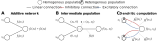
\includegraphics{media/chapters/03_nlif/03_01/nef_multivariate_functions.pdf}%
	{\phantomsubcaption\label{fig:nef_multivariate_functions_a}}%
	{\phantomsubcaption\label{fig:nef_multivariate_functions_b}}%
	{\phantomsubcaption\label{fig:nef_multivariate_functions_c}}%
	\caption[Using dendritic computation to compute multivariate functions in the NEF]{Using dendritic computation to compute multivariate functions in the NEF. \textbf{(A)} Standard NEF networks are additive: summation in activity space corresponds to addition in representation space.
	\textbf{(B)} Computing nonlinear multivariate functions $\phi$ generally requires all variables to be represented in an intermediate population.
	\textbf{(C)} The dendritic computation scheme discussed in here.
	Two pre-populations project onto a post-population with separate excitatory and inhibitory input channels.
	%The nonlinear interaction between these channels is exploited to compute $\phi$.
	}
	\label{fig:nef_multivariate_functions}
\end{figure}

The idea of dendritic computation as pursued here is best explained by exploring how mul\-ti\-va\-ri\-ate functions such as $\phi(x_1, \ldots, x_\ell)$ can be computed in the NEF, and by reviewing some fundamental theoretical properties of neural networks.
Specifically, we analyse three different network architectures (cf.~\Cref{fig:nef_multivariate_functions}).
\enquote{Additive networks} represent the variables $x_1$, $\ldots$, $x_\ell$ in independent neuron populations and cannot approximate most multivariate functions.
In contrast, networks with an intermediate population representing all variables at the same time are universal function approximators.
Dendritic computation relies on non-linear interaction between independent neural input channels.
While not as powerful as networks with an intermediate population, dendritic computation can approximate larger classes of functions well compared to additive networks.

\subsection{Additive Multivariate Networks}
\label{sec:additive_net}

As stated above, our goal is to compute multivariate functions $\phi(x_1, \ldots, x_\ell)$ within the context of the NEF.
%For the sake of simplicity, we mostly discuss bivariate functions of the form $\phi(x_1, x_2)$, but the same considerations apply to more than two input variables as well.
For the sake of simplicity, assume that two pre-populations representing the variables $x_1$, $x_2$ are connected to a common post-population.
To compute $\phi(x_1, x_2)$, we must find connection weights $\vec w_{1, i}$, $\vec w_{2, i}$ such that the following holds for every post-neuron $i$
\begin{align}
	a_i(\phi(x_1, x_2))
		= G_i \bigl[
			\langle \vec e_i, \phi(x_1, x_2) \rangle
		\bigr]
		\supposedEq G_i\bigl[
			\langle \vec w_{1, i}, \vec a^\mathrm{pre}_1(x_1) \rangle + \langle \vec w_{2, i}, \vec a^\mathrm{pre}_2(x_2)
		\rangle\bigr] \,.
	\label{eqn:nef_multivariate_addition}
\end{align}
Here, $a_i$ is the desired post-neuron activity according to the normative tuning-curve constraint (eq.~2.??).
% TODO: Add correct reference
As discussed in the context of the NEF transformation principle in Section~2.3.5, we assume that the current-translation function $J_i$ is part of the individual neuron response curve $G_i$, and that the currents induced by the pre-populations are summed.
% TODO: Add correct reference

Now, consider multivariate functions that can be decomposed into a sum of two univariate functions, i.e., $\phi(x_1, x_2) = f_1(x_1) + f_2(x_2)$ (\Cref{fig:nef_multivariate_functions_a}).
We can easily find weights $\vec w_{1, i}$, $\vec w_{2, i}$ that approximate such a function using the encoder-decoder split of the NEF.
Computing function decoders $\mat D^{f_1}$, $\mat D^{f_2}$ and using the identity $(\vec w_i)^T = \vec e_i \mat D$, we have
\begin{align*}
	G_i\bigl[
	  \langle
	  	\vec e_i \mat D^{f_1},
	  	\vec a^\mathrm{pre}_1(x_1)
	  \rangle
	+ \langle
	  	\vec e_i \mat D^{f_2},
		\vec a^\mathrm{pre}_2(x_2)
	\rangle\bigr] = 
	G_i\bigl[\langle \vec e_i, \mat D^{f_1} \vec a_1^\mathrm{pre}(x_1) + \mat D^{f_2} \vec a_2^\mathrm{pre}(x_2) \rangle\bigr]
	\approx a_i\bigl(f_1(x_1) + f_2(x_2)\bigr) \,.
\end{align*}
This equation can be interpreted as saying that addition in activity space (i.e., summing weighted pre-activities, eq.~\ref{eqn:nef_multivariate_addition}) is equal to addition in represented space.
In other words, standard NEF networks are \emph{additive}.
%\footnote{We already used the additivity of NEF networks in~Section~2.3.5, when we discussed the dynamics principle.}
Summing functions incurs no additional decoding error.

\begin{figure}
	\centering
	\includegraphics{media/chapters/03_nlif/03_01/perceptron.pdf}%
	{\phantomsubcaption\label{fig:perceptron_a}}%
	{\phantomsubcaption\label{fig:perceptron_b}}%
	\caption[Additive networks are a generalisation of the perceptron]{Additive networks are a generalisation of the perceptron. \textbf{(A)} An additive network is a sum of arbitrary univariate functions. \textbf{(B)} A perceptron is an additive network with functions of the form $f_i(x_i) = w_i x_i + \beta \ell^{-1}$. The weights $w_i$ are learned such that the output approximates a desired function.}
\end{figure}

\subsubsection{Additive networks cannot compute most multivariate functions}
The only way to compute general multivariate functions $\phi(x_1, x_2)$ in additive networks is to \emph{approximate} $\phi$ as an additive univariate decomposition.
As expressed by the following theorem (see Appendix~B.3.1 for a proof), it is \emph{impossible} to compute many continuous multi-variate $\phi$ using such additive networks.%
\footnote{We limit Theorem~\ref{thm:xor_general} to continuous functions for the sake of simplicity.
However, we conjecture that the same results hold for larger classes of functions, for example square Lebesgue integrable functions.}
This is true even if we can decode arbitrary univariate functions $f_1$, $\ldots$, $f_\ell$ over the pre-variables (this is equivalent to having an infinite number of pre-neurons, see below), and we were able to freely choose a fixed nonlinearity $\sigma$ (cf.~\Cref{fig:perceptron_a}).

\begin{theorem}
\label{thm:xor_general}
Let $\ell > 1$, $\Xrepr \subset \mathbb{R}^\ell$ and $\mathbb{Y} \subset \mathbb{R}$ be compact sets, and $\sigma$, $\phi$, $f_i$ be continuous.
For any fixed $\sigma : \mathbb{R} \longrightarrow \mathbb{Y}$, there always exist $\phi : \Xrepr \longrightarrow \mathbb{Y}$ such that there are no $f_1$, $\ldots$, $f_\ell : \mathbb{R}  \longrightarrow \mathbb{R}$ with the property
$\phi(x_1, \ldots, x_\ell) = \sigma(\xi) = \sigma\bigl( f_1(x_1) + \ldots + f_\ell(x_\ell) \bigr)$ for all $(x_1, \ldots, x_\ell) \in \Xrepr$.
\end{theorem}

\begin{figure}
	\centering
	\includegraphics{media/chapters/03_nlif/03_01/xor_visualisation.pdf}%
	{\phantomsubcaption\label{fig:xor_visualisation_a}}%
	{\phantomsubcaption\label{fig:xor_visualisation_b}}%
	{\phantomsubcaption\label{fig:xor_visualisation_c}}%
	{\phantomsubcaption\label{fig:xor_visualisation_d}}%
	{\phantomsubcaption\label{fig:xor_visualisation_e}}%
	\caption[Visualisation of the XOR decision problem for different classifiers]{Visualisation of the XOR decision problem for different classifiers. The goal is to find classifier parameters such that the four samples are classified as depicted.
	The background corresponds to the sign of the monotonic function $\sigma(\xi)$.
	\textbf{(A)} The linear decision boundary formed by the Perceptron cannot solve the XOR problem.
	\textbf{(B)} This holds for any function of the form $\sigma(f_1(x_1) + f_2(x_2))$, here $f_1(x_1) = \cos(2\pi x_1)$ and $f_2(x_2) = \sin(2\pi x_2)$.
	\textbf{(C)} A multi-layer Perceptron (MLP) of the form $\sum_i w_i \sigma(e_i^1 x_1 + e_i^2 x_2 + \beta_i )$ can solve the problem, although the decision boundary is quite erratic.
	\textbf{(D)} An alternative solution using the nonlinearity $\sigma'(\xi) = \sigma(\xi^2 - 1)$.
	\textbf{(E)} Multiplication of two real-valued variables $x_1$, $x_2$ can be seen as a continuous form of the XOR problem.
	Additive networks cannot compute this function.
	}
	\label{fig:xor_visualisation}
\end{figure}

\subsubsection{The Perceptron and XOR}
Consider monotonic $\sigma$ and affine $f_i$ of the form $w_i x_i + \beta \ell^{-1}$.
We obtain the \emph{perceptron}, an early single-layer neural network (cf.~\Cref{fig:perceptron_b}; \cite{rosenblatt1958perceptron}).
\Citet[Chapter~2; originally published in 1969]{minsky1987perceptrons} point out that such networks cannot compute the boolean XOR function (\Cref{fig:xor_visualisation_a}).%
\footnote{\Citet{minsky1987perceptrons} note that the perceptron was proved by Rosenblatt to \enquote{learn to do anything it was possible to program it to do}; this ambiguous statement endowed researchers with a surplus of optimism---especially since perceptrons could sometimes learn to solve difficult problems.
Among other factors, realising that these networks could not be \emph{programmed} to solve a simple problem such as XOR led to what some call \enquote{the first AI winter} \citep[e.g.,][]{muthukrishnan2020brief}.}
%In the continuous domain, the same is true for multiplication over $\mathbb{X} = [-1, 1]^2$, that is $\phi(x_1, x_2) = x_1 x_2$ (\Cref{fig:xor_visualisation_a}).
Even the general additive networks from our theorem cannot solve a \emph{weaker} version of the XOR problem, formalised below.

\begin{definition}
\label{def:weak_xor}
A function $\phi(x, y)$ solves the \emph{weak XOR problem} if there exist $a_0, b_0, a_1, b_1$ with
\begin{align*}
	\big( \phi(a_0, b_0) < \phi(a_0, b_1) \big) \wedge
	\big( \phi(a_1, b_1) < \phi(a_0, b_1) \big) \wedge
	\big( \phi(a_0, b_0) < \phi(a_1, b_0) \big) \wedge
	\big( \phi(a_1, b_1) < \phi(a_1, b_0) \big) \,.
\end{align*}
\end{definition}
That is, we merely require $\phi(a_0, b_0)$ and $\phi(a_1, b_1)$ to be larger than $\phi(a_0, b_1)$ and $\phi(b_1, b_0)$.

\begin{restatable}{theorem}{ThmWeakXor}
\label{thm:weak_xor}
Let $\sigma$ be monotonic. Then, an additive network of the form $\phi(x_1, x_2) = \sigma(f_1(x_1) + f_2(x_2))$ cannot solve the weak XOR problem.
\end{restatable}
This may be surprising, given that, as depicted in \Cref{fig:xor_visualisation_b}, we can generate highly nonlinear classification boundaries.
We provide a proof in Appendix~B.3.2.

To solve the XOR problem, we can either, as discussed next, use multi-layer networks (cf.~\Cref{fig:xor_visualisation_c}), or, alternatively make $\sigma$ non-monotonic.
As depicted in \Cref{fig:xor_visualisation_d}, setting $\sigma(\xi) = \xi^2 - 1$ allows us to solve the XOR problem.
This illustrates our goal with dendritic computation: exploit \enquote{more powerful} $\sigma$ to approximate a larger class of functions.

Still, the functions that we can compute using additive networks are limited, even if we can freely choose $\sigma$.
For example, we can compute $x_1 x_2$ for $(x_1, x_2) \in [\epsilon, 1]^2$ and $0 < \epsilon < 1$ by setting $f_1$ and $f_2$ to the logarithm and $\sigma$ to the exponential.
However, it is impossible to find functions that compute multiplication over all four quadrants---which can be seen as a continuous version of the XOR problem (\Cref{fig:xor_visualisation_e}).
More precisely, allowing $x_1$, $x_2$ to be zero makes it impossible to compute multiplication in these networks (proof in Appendix~B.3.3).
\begin{restatable}{theorem}{ThmMultiplication}
\label{thm:multiplication}
There are no continuous, real-valued functions $f_1$, $f_2$, $\sigma$ such that $\sigma(f_1(x_1) + f_2(x_2)) = x_1 x_2$ for all $(x_1, x_2) \in [0, 1]^2$.
\end{restatable}


%Choosing this $\sigma$ implicitly introduces a non-linear interaction between the variables $x_1$, $x_2$, for example
%\begin{align*}
%	\sigma\left( (w_1 x_1 + w_2 x_2 + \beta)^2 - 1\right) = 
%	\sigma\left( w_1^2 x_1^2 + w_2^2 x_2^2 + 2 w_1 w_2 x_1 x_2 + 2 w_1 \beta x_1 + 2 w_2 \beta x_2 + \beta^2  - 1\right) \,.
%\end{align*}
%The product-term $w_1 w_2 x_1 x_2$ can be exploited to %compute multiplication-like functions.
%Still, as stated in Theorem~1, there inevitably is a large set of functions that we cannot compute.
% TODO Add reference

\subsection{Multi-Layer Networks}

\begin{figure}
	\includegraphics{media/chapters/03_nlif/03_01/mlp.pdf}
	\caption[Sketch of a two-layer neural network]{Sketch of a two-layer neural network with rectified linear units (ReLUs). If the encoding vectors $\vec e_i$ and the biases $\beta_i$ are sampled appropriately, this network is a universal function approximator.}
	\label{fig:mlp}
\end{figure}

As already mentioned in Section~2.3.5, an individual NEF population can be interpreted as a two-layer neural network (cf.~\Cref{fig:mlp}).
% TODO: Add reference
As long as the encoding vectors are sampled from $\ell$-dimensional hypersphere and $x$-intercepts are uniformly distributed, such a neuron population is a universal function approximator.
The following theorem states this more formally for neurons with a rectified linear unit (ReLU) nonlinearity, i.e., $\sigma(\xi) = \max\{0, \xi\}$.

\begin{theorem}
\label{thm:two_layer_universal}
Let $\ell \geq 1$, and $\phi : \mathbb{B}^\ell \longrightarrow \mathbb{R}$ be a continuous function mapping from the $\ell$-dimensional unit ball onto $\mathbb{R}$.
Furthermore, let $\sigma(\xi) = \max\{0, \xi\}$, $\vec e_i$ be sampled uniformly from the unit-sphere $\mathbb{S}^\ell$, and $\beta_i$ be sampled uniformly from $[-1, 1]$.
There exist $d_i \in \mathbb{R}$ such that
\begin{align}
	\phi(\vec x) = \lim_{\Npop \to \infty} \sum_{i = 1}^{\Npop} d_i \sigma\bigl( \langle \vec e_i, \vec x \rangle + \beta_i \bigr) \quad \text{for all} \quad \vec x \in \mathbb{B}^\ell \,.
	\label{eqn:two_layer_network}
\end{align}
\end{theorem}

This follows from \citet{hornik1989multilayer}.
We provide a sketch of a proof in Appendix~B.3.3.
This theorem can be easily extended to hold for arbitrary compact domains $\Xrepr$, codomain dimensionalities, and other neural nonlinearities $\sigma$.

%It may not be obvious why \cref{eqn:two_layer_network} describes a \enquote{two-layer} neural network.
%In essence, the encoding weights $\vec e_i$ map $\vec x$ onto the input of one of the $N$ neurons with nonlinearity $\sigma$.
%This step forms the \enquote{first} or \enquote{hidden layer}.
%The decoding weights $d_i$ then map the neural activities $\sigma(\xi_i)$ onto the output, which forms the \enquote{second layer} (cf.~Figure~2.20).
%% TODO: Add actual reference

\subsubsection{The role of uniformly sampled encoders}
Theorem~\ref{thm:two_layer_universal} requires that the encoding vectors $\vec e_i$ are uniformly sampled from the hypersphere $\mathbb{S}^\ell$.%
\footnote{As follows from the proof of Theorem~\ref{thm:two_layer_universal} in Appendix~B.3.3, there technically are weaker requirements for this.
One example is given in \citet{gosmann2015precise}; given a specific function $\phi$ (such as multiplication), there are certain distributions of encoding vectors that minimise the decoding error.
In fact, global optimisation methods such as stochastic gradient descent can be seen as systematically selecting such \enquote{optimal} encoders.}
To get an intuition as for why this is important, consider the case where the $\vec e_i$ are axis-aligned, i.e., $\|\vec e_i\|_0 = 1$ (cf.~Appendix~A.1).
% TODO: Add reference for zero-norm in Appendix~A.1
In this case, we can split \cref{eqn:two_layer_network} into $\ell$ sub-networks, each decoding a function over a single variable $x_\ell$
\begin{align*}
		\sum_{i = 1}^N d_i \sigma\bigl( \langle \vec e_i, \vec x \rangle - \beta_i \bigr)
	= 	\sum_{j = 1}^\ell \sum_{i = 1}^{N_j} d_{j i} \sigma\bigl( e_{j i} x_j - \beta_{j i} \bigr) \,, \text{where } e_{j i} \in \{ -1, 1\} \,.
\end{align*}
This is equivalent to the additive networks we discussed before.
We can only decode sums of univariate functions over the individual $x_j$ from the pre-population.

\subsubsection{Intermediate populations}
%We now know that we can indeed approximate multivariate functions in the NEF with an arbitrarily small error.
%The pre-condition for this is that all variables over which we would like to compute a $\phi$ represented in the same neuron population with non-axis aligned encoding vectors $\vec e_i$.
As discussed by \citep[Chapter~6]{eliasmith2003neural}, we need to introduce intermediate populations if, as an example, variables $x_1$, $x_2$ are represented in independent pre-populations, and we would like to compute a multivariate function $\phi(x_1, x_2)$.
This intermediate population represents a vectorial quantity $\vec z = (x_1, x_2)$ (cf.~\Cref{fig:nef_multivariate_functions_b}).
This can be accomplished by computing the univariate functions $f_1(x_1) = (x_1, 0)$ and $f_2(x_2) = (0, x_2)$ in the connections to the intermediate population.
According to Theorem~\ref{thm:two_layer_universal} we can then decode any multivariate function from the intermediate population.

\subsubsection{Potential issues with intermediate populations}
In theory, the number of neurons required to cover a $d$-dimensional space is exponential in $d$.
Representing a $d$-dimensional quantity in an intermediate population thus requires many neurons to achieve a certain decoding error.
In practice, it is quite difficult to judge the number of neurons required to decode a certain function $f$ a-priori; the decoding error heavily depends on $f$ and the encoding vectors $\vec e_i$.

Another problem arises when modelling neurobiological systems.
There may be no indication that an intermediate population exists in a particular biological circuit, but the function can be modelled well as a multivariate function.
An example of this would be the aforementioned attention system, where a group of control neurons modulates another population without an intermediary \citep{bobier2014unifying}.

Finally, there is the issue of noise.
In spiking neural networks, every intermediate neuron population introduces additional noise due to static distortion and spike noise \citep[Section~2.2.2]{eliasmith2003neural}.
We see the effects of this later.

\subsection{Dendritic Computation}
\label{sec:dendritic_computation_theory_dendritic}

Dendritic computation is one way to partially alleviate the limitations arising from intermediate populations.
The basic idea is that each neuron possesses $k$ \emph{input channels}.
Input fed through these channels interacts nonlinearly, modelling information processing within the dendrites.

\begin{figure}
	\includegraphics{media/chapters/03_nlif/03_01/dendritic_computation.pdf}%
	{\phantomsubcaption\label{fig:dendritic_computation_net}}%
	{\phantomsubcaption\label{fig:dendritic_computation_fun}}%
	\caption[Overview of our notion of dendritic computation.]{Overview of our notion of dendritic computation. \textbf{(A)} Neuron with an excitatory and inhibitory input channel. In a network context, these functions are decoded from pre-populations representing these variables. Connectivity can be constrained such that excitatory and inhibitory pre-neurons only connect to the corresponding channel. \textbf{(B)} Conceptually, each channel receives a sum of univariate functions computed over the pre-variables $x_1$, $\ldots$, $x_\ell$.}
\end{figure}

Mathematically, the response curve describing the average neural activity is now a multivariate function $\mathscr{G}[\xi_1, \ldots, \xi_k]$, where the $\xi_i$ are linear combinations of the pre-activities (\Cref{fig:dendritic_computation_net}).
To compute $\phi(x_1, \ldots, x_\ell)$, the following must hold for each post-neuron $i$
\begin{align}
	\begin{aligned}
	a_i\bigl(\phi(x_1, \ldots, x_\ell)\bigr) &\supposedEq
	\mathscr{G} \bigl[
		\langle \vec w_{1, i}^1, \vec a^\mathrm{pre}_1(x_1) \rangle + \ldots +
		\langle \vec w_{\ell, i}^1, \vec a^\mathrm{pre}_\ell(x_\ell) \rangle, \ldots,\\
%	&~\quad\quad\vdots, \\
	&~\hspace{1.66em}
		\langle \vec w_{1, i}^k, \vec a^\mathrm{pre}_1(x_1) \rangle + \ldots +
		\langle \vec w_{\ell, i}^k, \vec a^\mathrm{pre}_\ell(x_\ell) \rangle
	\bigr]
	\end{aligned}
	\label{eqn:dendritic}
\end{align}
where $a_i(\phi(x_1, \ldots, x_\ell))$ expresses the normative tuning constraint defined in Section~2.3.2.
% TODO: Add correct reference

Note that we deliberately left the concept of an \enquote{input channel} a little vague.
An input channel could either refer to a different location in the dendritic tree, different synapse types (e.g., excitatory or inhibitory synapses), or even the effects of signalling molecules such as hormones.
We discuss examples of model neurons with multiple input channels in \Cref{sec:nlif}.

\subsubsection{Mathematical analysis}
More formally, using $\sigma(\xi_1, \ldots, \xi_\ell)$ as an abstract nonlinearity and assuming that we can compute any univariate function $g_i^j$ over $\xi_1, \ldots, \xi_\ell$, we have (\Cref{fig:dendritic_computation_fun})
\begin{align}
	\sigma \bigl(
		g_{1}^1(x_1) + \ldots + g_{\ell}^1(x_\ell), \ldots, g_{1}^k(x_1) + \ldots + g_{\ell}^k(x_\ell)
	\bigr) = \phi(x_1, \ldots, x_\ell) \,.
	\label{eqn:dendritic_computation_theory}
\end{align}
Such networks are more powerful than additive networks.
For example, let $\sigma(\xi_1, \xi_2) = \xi_1 \xi_2$.
Now, if we set the functions feeding into the second channel to one, i.e., $g_{1, i}^2(x_1) = \ldots = g_{\ell, 1}^2(x_\ell) = 1$, we obtain an additive network.
Of course, using the same $\sigma$, we can, in contrast to additive networks, compute products of the pre-variables over arbitrary domains.

Still, independent of $\sigma$, and similarly to additive networks, dendritic computation networks are not universal function approximators (see Appendix~B.3.5~for the theorem and proof).

%\begin{theorem}
%\label{thm:dendritic_compuation_incomplete}
%Let $\ell > 1$, $\Xrepr \subset \mathbb{R}^\ell$ and $\mathbb{Y} \subset \mathbb{R}$ be compact sets, and $\sigma$, $\phi$, $g^j_i$ be continuous.
%For any fixed $\sigma : \mathbb{R}^k \longrightarrow \mathbb{Y}$, there always exist $\phi : \Xrepr \longrightarrow \mathbb{Y}$ such that there are no $g^1_1$, $\ldots$, $g^k_\ell : \mathbb{R}  \longrightarrow \mathbb{R}$ with the property
%$\phi(x_1, \ldots, x_\ell) = \sigma(\xi_1, \ldots, \xi_k) = \sigma\bigl( g^1_1(x_1) + \ldots + g^1_\ell(x_\ell), \ldots,  g^k_1(x_1) + \ldots + g^k_\ell(x_\ell)\bigr)$ for all $(x_1, \ldots, x_\ell) \in \Xrepr$.
%\end{theorem}

%\subsubsection{Interaction between excitation and inhibition}
%\Cref{fig:nef_multivariate_functions_c} shows an example of a neural network exploiting nonlinear interactions between excitatory and inhibitory synapses.
%Assume that each neuron in the post population possesses an independent excitatory and inhibitory channel, and that the two pre-population represent $x_1$, $x_2$, respectively, and project onto both channels.
%The activity of a single post-neuron $i$ is hence given as
%\begin{align*}
%	\mathscr{G}_i\bigl[
%		\langle
%			\vec w^1_\mathrm{E},
%			\vec a_\mathrm{pre}^1(\vec x_1)
%		\rangle + \langle
%			\vec w^2_\mathrm{E},
%			\vec a_\mathrm{pre}^2(\vec x_2)
%		\rangle,
%		\langle
%			\vec w^1_\mathrm{I},
%			\vec a_\mathrm{pre}^1(\vec x_1)
%		\rangle + \langle
%			\vec w^2_\mathrm{I},
%			\vec a_\mathrm{pre}^2(\vec x_2)
%		\rangle
%	\bigr] \,,
%\end{align*}
%where $\vec w_\mathrm{I}$ and $\vec w_\mathrm{E}$ are the excitatory and inhibitory synaptic weights, and $\vec a_\mathrm{pre}$ are the activities of the pre-populations.
%Assuming that we can decode arbitrary univariate functions over $x_1$, $x_2$ from the pre-populations, our goal is to find functions $g_\mathrm{E}^1(x_1)$, $g_\mathrm{E}^2(x_2)$, $g_\mathrm{I}^1(x_1)$, $g_\mathrm{I}^2(x_2)$, such that the total activity of our neuron has some desired value, i.e.,
%\begin{align*}
%	a_i^\mathrm{post}(\phi(x_1, x_2)) \supposedEq \mathscr{G}_i\bigl[
%		g_\mathrm{E}^1(x_1) + g_\mathrm{E}^2(x_2),
%		g_\mathrm{I}^1(x_1) + g_\mathrm{I}^2(x_2)
%	\bigr] \,.
%\end{align*}


\subsection{Numerical Exploration}
\label{sec:dendritic_computation_theory_numerical}

The above considerations are quite theoretical and provide only limited insight into the practical impact of choosing one network type over the other.
In this section, we discuss a simple numerical experiment that highlights the function approximation errors obtained with different network types for functions $\phi$ of varying \enquote{complexity}.
We use experiments similar to the following throughout this chapter to characterise different network- and neuron-types.

\begin{figure}
	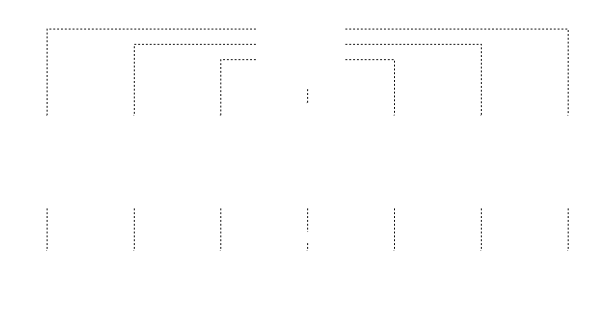
\includegraphics{media/chapters/03_nlif/03_01/2d_functions_overview_overlay.pdf}%
	\kern-157.24mm\includegraphics{media/chapters/03_nlif/03_01/2d_functions_overview.pdf}
	\caption[Overview of our procedure for generating random 2D functions]{Overview of our procedure for generating random 2D functions. \textbf{(A)} We sample a 2D array from a normal distribution (size of the array depends on the filter width; negative values in red, positive in blue). \textbf{(B)} The noise is filtered by convolving with a Gaussian kernel with standard-deviation $\sigma$ (for large filter widths, i.e., small $\sigma^{-1}$, only a small portion of the filter is depicted). \textbf{(C)} The resulting functions are transformed to have mean zero (i.e., no DC component) and a standard deviation of one.}
	\label{fig:2d_functions_overview}
\end{figure}

To analyse different network architectures, w
e randomly generate two-dimensional functions $\phi(x_1, x_2)$ from band-limited white noise with standard deviation one and mean zero.
The band-limit is enforced by filtering with a Gaussian filter kernel with standard deviation $\sigma$.
This is depicted in \Cref{fig:2d_functions_overview}.
Large $\sigma$ result in functions with no high frequencies; such functions are approximately linear.
In contrast, small $\sigma$ result in quite intricate random structures.
Correspondingly, $\sigma^{-1}$ can be seen as a proxy for the \enquote{complexity} of a function.
Small $\sigma^{-1}$ result in low-complexity functions, large $\sigma^{-1}$ in high-complexity functions.


%\clearpage
%% !TeX spellcheck = en_GB

\section{Extending the Neural Engineering Framework}
\label{sec:nef_extension}

Up to this point, we have formally defined dendritic computation and discussed its theoretical benefits.
The goal of this section is to open avenues toward systematically integrating multi-compartment neuron models with dendritic trees into \NEF networks using the formalisms discussed above.

Na\"ively, incorporating neurons with multiple nonlinear input channels into the \NEF is merely a matter of solving for $\vec w$ such that \Cref{eqn:dendritic} holds.
Phrasing this as an optimisation problem, we must minimise the difference between the desired average activity according to the normative tuning-curve constraint $a_i(\vec x)$, and the average activity according to our multivariate response curve $\mathscr{G}$.
Using a least-squares loss (and omitting the regularisation term), we have
\begin{align}
	\begin{aligned}
	E &=
	\frac{1}{\vol(\Xrepr)} \int_{\Xrepr} \Bigl( a_i\bigl(\phi(x_1, \ldots, x_\ell)\bigr) -
	\mathscr{G} \bigl[
		\langle \vec w_{1, i}^1, \vec a^\mathrm{pre}_1(x_1) \rangle + \ldots +
		\langle \vec w_{\ell, i}^1, \vec a^\mathrm{pre}_\ell(x_\ell) \rangle, \ldots,\\
	&~\hspace{13.825em}
		\langle \vec w_{1, i}^k, \vec a^\mathrm{pre}_1(x_1) \rangle + \ldots +
		\langle \vec w_{\ell, i}^k, \vec a^\mathrm{pre}_\ell(x_\ell) \rangle
	\bigr] \Bigr)^2 \, \D x_1 \ldots \D x_\ell \,.
	\end{aligned}
	\label{eqn:dendritic_computation_optimisation}
\end{align}
One way to minimise this loss-function would be to use stochastic gradient descent.
In fact, this can be a viable strategy---and may be the only option for many detailed neuron models.

Still, we would like to suggest a more systematic approach that, in some cases, reduces the task of finding weights to a convex \qprog.
This is more in line with the \enquote{standard} \NEF, where connection weights are computed by solving a convex least-squares problem.

To arrive at a point where we can integrate complex neuron models more seamlessly, we first need to address two of the limitations of the \NEF discussed in \Cref{sec:nef_limitations}.
Specifically, we discuss how to eliminate the bias currents and to account for Dale's principle.
Furthermore, we present a modified version of \Cref{eqn:dendritic_computation_optimisation} that splits the multivarite response curve $\mathscr{G}$ into a multivariate input-dependent nonlinearity $H$ and a univariate response curve $G$.
We avoid decoding subthreshold currents using a technique we call \enquote{subthreshold relaxation}.

\subsection{Decoding the Current-Translation Function}
\label{sec:nef_decode_current}

So far we assumed that the current translation function $J_i(\xi)$ is an intrinsic part of the neuron model.
Our typical choice of $J_i(\xi) = \alpha_i \xi + \beta_i$ introduces a bias current $\beta_i$ into each neuron.
As we elaborated in \Cref{sec:nef_limitations}, this is slightly implausible from a biological perspective.

\Citet{tripp2007neural} demonstrate that it is possible to robustly solve for synaptic weights that approximate arbitrary post-synaptic current functions.
We use this insight to directly approximate the target current $J_i(\langle \vec e_i, \vec x \rangle)$; as a side effect, we implicitly solve for the bias.
Again, assuming that the post-synaptic current is linear in the pre-population activities, we must find a weight vector $\vec w_i$ such that the following regularised loss is minimised
\begin{align}
E = \frac{1}{\vol(\Xrepr)} \int_{\Xrepr} \left( J_i\bigl(\langle \vec e_i, \phi(\vec x)\rangle\bigr) - \langle \vec w_i, \vec a^\mathrm{pre}(\vec x) \rangle \right)^2 \, d\vec x + \lambda \| \vec w_i \|_\mathrm{2}^2\,.
\label{eqn:decode_current}
\end{align}
As before, this equation can be discretised, brought into canonical least squares form, and solved using the regularised Moore-Penrose pseudo inverse (cf.~eqn.~2.22 and 2.23):
\begin{align*}
	\mat W &= \mat A^+ \mat J \,, & \text{where} \quad \mat A^+ &= (\mat A^T \mat A + \lambda N \mat I)^{-1} \mat A^T \,.
\end{align*}
Here, $N$ is the number of samples, $\mat W \in \mathbb{R}^{m \times \Npop}$ is the connection weight matrix, $\mat J \in \mathbb{R}^{N \times m}$ is a matrix of target currents, and $\mat A \in \mathbb{R}^{N \times n}$ is the matrix of pre-activities.

\begin{figure}
	\includegraphics{media/chapters/03_nlif/03_02/current_translation_decoding.pdf}%
	{\phantomsubcaption\label{fig:current_translation_decoding_a}}%
	{\phantomsubcaption\label{fig:current_translation_decoding_b}}%
	{\phantomsubcaption\label{fig:current_translation_decoding_c}}%
	{\phantomsubcaption\label{fig:current_translation_decoding_d}}%
	\caption[Decoding for currents instead of represented values]{Decoding for currents instead of represented values. \textbf{(A)} Tuning curves of a pre-population with $100$ \LIF neurons (only $50$ tuning curves are shown). \textbf{(B)} Decoding affine current translation functions $J_i$ (dotted lines are the target). The function $\phi$ being computed in re\-pre\-sen\-tat\-ion space is the identity function. Dashed line corresponds to the threshold current $J_\mathrm{th} = \SI{1}{\nano\ampere}$.
	\textbf{(C)} Same as \emph{(B)} but for Gaussian current-translation functions $J_i$. Such functions can be used to produce localised tuning curves.
	\textbf{(D)} First six singular values of the two weight matrices $\mat W$ from \emph{(B, C)}.
	Singular values are normalised by dividing by their sum, resulting in the relative contribution of each singular value to the decoding.
	For affine $J_i$, $\mat W$ is of rank $d + 1$ (here $d = 1$);
	Gaussian $J_i$ result in full-rank $\mat W$.
	}
\end{figure}

Importantly, we no longer solve for weights directly in the domain of represented values $\vec x$; this is in contrast to solving for decoders $\mat D$ according to \cref{eqn:lstsq_loss}.
Similarly, we do not solve for target activities $a_i$, as was suggested by our na\"ive loss function in \cref{eqn:dendritic_computation_optimisation}.
Side-stepping the neural nonlinearity $G$ enables a simple least-squares solution.
Furthermore, this optimisation scheme supports arbitrary current-translation functions $J_i$, providing modellers with a greater flexibility over the tuning curve constraint (cf.~\Cref{fig:current_translation_decoding_a,fig:current_translation_decoding_b,fig:current_translation_decoding_c}).

\subsubsection{Low-rank factorisation of $\mat W$}
Solving the optimisation problem in \cref{eqn:decode_current} directly results in a weight matrix $\mat W$ instead the low-rank factorisation $\mat W = \mat E \mat D^\phi$.
As discussed in \Cref{sec:nef_transformation}, this factorisation was useful, since it enables $\mat W \vec a$ to be computed in $\mathcal{O}(n)$ instead of $\mathcal{O}(n^2)$.

Fortunately, at least in the case of the affine current-translation function $\alpha_i \langle \vec e_i, \phi(\vec x) \rangle + \beta_i$, we still obtain a factorisable matrix (cf.~\Cref{fig:current_translation_decoding_d}).
The resulting $\mat W$ is merely of rank $d + 1$, where $d$ is the dimensionality of the post-population.
Specifically, the weight matrix can be expressed as a sum of the low-rank factorisation $\mat E \mat D^\phi$ and the outer product of the biases $\vec \beta \in \mathbb{R}^{m \times 1}$ with a decoding vector $\mat D^1 \in \mathbb{R}^{1 \times n}$.
This \enquote{bias-decoder} decodes the constant \enquote{one} from the pre-population.
In other words, it simply holds $\mat W = \mat E \mat D^\phi + \vec \beta \mat D^1$ (cf.~\cite[Chapter~4]{stockel2017point,duggins2017incorporating}).

\begin{figure}
	\includegraphics{media/chapters/03_nlif/03_02/bias_decoding_impact.pdf}%
	{\phantomsubcaption\label{fig:bias_decoding_impact_a}}%
	{\phantomsubcaption\label{fig:bias_decoding_impact_b}}%
	{\phantomsubcaption\label{fig:bias_decoding_impact_c}}%
	{\phantomsubcaption\label{fig:bias_decoding_impact_d}}%
	\caption[Bias decoding and post-population tuning curve accuracy]{Bias decoding and post-population tuning curve accuracy. \textbf{(A)} Pre-population tuning-curves for $n = 50$ \LIF neurons.
	\textbf{(B)}~Error for decoding the identity function compared to decoding a constant (regularisation factor $\sigma = 10$). The error for decoding a constant is minimally larger than that for decoding the identity function.
	\textbf{(C)}~The first four principal components of the tuning curves (for $n = 1000$).
	The principal components resemble the Legendre polynomials, an orthogonal function basis (dotted lines).
	\textbf{(D)} \RMSE between the desired post-population tuning and the actually achieved tuning. Decoding the bias approximately doubles the error compared to intrinsic bias currents.}
\end{figure}

\subsubsection{Impact of decoding bias currents on network function}
%It is difficult to make blanket statements about the impact of bias decoding on the network function.
Generally speaking, decoding biases increases the error between the actual and desired post-population tuning.
The magnitude of this error depends on the pre- and post-population. 
The former determine how well a constant offset can be decoded, the latter determine the magnitude of the required bias currents.

In the case of \enquote{standard} \NEF tuning with uniform $x$-intercepts and random encoders (cf.~\Cref{fig:bias_decoding_impact_a}), constant functions can, counter-intuitively, only be decoded with a slightly higher error than the identity function (error is about $15\%$ higher; cf.~\Cref{fig:bias_decoding_impact_b}).
This becomes apparent when considering the principal components of the pre-population tuning curves.
As, for example, discussed in \citet[Chapter~7]{eliasmith2003neural}, the principal component analysis (PCA) can be seen as \enquote{uncovering} the best orthogonal basis that linearly generates the tuning-curves.
%(see \cite[Chapter~12]{bishop2006pattern} for general information on the PCA).
In turn, the first principal components characterise the functions that can be decoded well from a population.
As illustrated in \Cref{fig:bias_decoding_impact_c}, the principal components $f_i$ of the \enquote{standard} \NEF tuning curves resemble the Legendre polynomials (cf.~\Cref{sec:function_bases} for a definition).
While the second principal component $f_2$ is linear, just like the corresponding Legendre polynomial, $f_1$ differs significantly from the constant first Legendre polynomial.
Decoding constants is hence \enquote{more difficult} than decoding the identity function.

In our example, and as depicted in \Cref{fig:bias_decoding_impact_d}, decoding $J_i$ doubles the \RMSE between the desired and actual post-population tuning.
%This can be countered by doubling the number of pre-neurons.
However, as we will see in the next subsection, there are circumstances where the absence of an intrinsic bias improves the network performance.

\subsubsection{Accounting for multiple pre-populations}
As we discussed in \Cref{sec:additive_net}, a welcome side effect of intrinsic current-translation is that standard \NEF networks are additive.
Summing the activities $\vec a^\mathrm{pre}_1$, $\ldots$, $\vec a^\mathrm{pre}_\ell$ from multiple pre-populations is equivalent to summing the decoded $f_1(\vec x_1)$, $\ldots$, $f_\ell(\vec x_\ell)$.
This is no longer the case when
%solving for weights $\vec w_i$
minimising the current-based loss in \cref{eqn:decode_current}.

\begin{figure}
	\includegraphics{media/chapters/03_nlif/03_02/nef_decode_bias.pdf}%
	{\phantomsubcaption\label{fig:nef_decode_bias_a}}%
	{\phantomsubcaption\label{fig:nef_decode_bias_b}}%
	{\phantomsubcaption\label{fig:nef_decode_bias_c}}%
	\caption[Accounting for multiple pre-populations when decoding the current-translation function]{Accounting for multiple pre-populations when decoding the current-translation function. \textbf{(A)} Biases can be manually distributed between pre-populations by scaling the bias decoders $\mat D^1_1$ and $\mat D^1_2$ by $\alpha$ and $(1 - \alpha)$, respectively. \textbf{(B)} The general solution is to solve for weights $\mat W$ assuming stacked pre-population activities. The two pre-populations form a \enquote{virtual} pre-population. \textbf{(C)} A combination of the two approaches, where only the bias $\mat D^1$ is decoded from the pre-populations in this way.}
\end{figure}

In the case of the affine $J_i$, each of the $\ell$ connections decodes the bias current, effectively multiplying the bias by $\ell$.
Of course, we can only decode a fraction of the bias from each pre-population (\Cref{fig:nef_decode_bias_a}).
Alternatively, we can combine the pre-populations into a \enquote{virtual pre-population} and let the optimisation process take care of distributing the responsibility for providing the bias between all pre-neurons (\Cref{fig:nef_decode_bias_b}).

More precisely, we explicitly solve for weights that result in $f_1(\vec x_1) + \ldots + f_\ell(\vec x_\ell)$ to be represented in the post-population.
For two populations, and skipping regularisation, we have
\begin{align}
	E =
	\frac{1}{\vol(\Xrepr)^2} \! \iint_{\Xrepr}
	\left(
		J_i\bigl(\langle \vec e_i, f_1(\vec x_1) + f_2(\vec x_2) \rangle\bigr)
		- \langle \vec w_{1, i}, \vec a_1^\mathrm{pre}(\vec x_1) \rangle
		- \langle \vec w_{i, 2}, \vec a_2^\mathrm{pre}(\vec x_2) \rangle
	\right)^2 \, \D\vec x_1 \D\vec x_2 \,.
	\label{eqn:decode_current_additive}
\end{align}
We can bring this problem into a canonical form by stacking the pre-activities and weights (see below for an example).
However, note that we now need to sample a much higher-dimensional space.
This is worrisome if we attempt to decode $f_i$ that must be finely sampled to obtain a good decoding.
Again, under the assumption that $J_i$ is affine, it is possible to expand the above integral and to solve for a---relatively easy to decode---population-spanning bias decoder $\mat D^1$ independent of the (untouched) function decoders $\mat D^{f_1}$ and $\mat D^{f_2}$ (\Cref{fig:nef_decode_bias_c}).

%\begin{align*}
%E^\beta &= \frac{1}{\vol(\Xrepr)^2} \! \int_{\Xrepr} \! \int_{\Xrepr} \left( \beta_i - \langle \vec w^\beta_{1, i}, \vec a_1^\mathrm{pre}(\vec x_1) \rangle - \langle \vec w^\beta_{i, 2}, \vec a_2^\mathrm{pre}(\vec x_2) \rangle \right)^2 \, d\vec x_1 \, d\vec x_2
%\end{align*}

\subsection{Nonnegative Weights and Dale's Principle}
\label{sec:nef_nonneg}

Biological neurons tend to follow Dale's principle---they act either excitatorily or inhibitorily (see~\Cref{sec:synaptic_transmission} for more detail).
As discussed in \Cref{sec:nef_limitations}, we ignored this in our weight-solving procedures.
Least-squares assigns arbitrary algebraic signs to the individual weights, typically with an even split between positive and negative (cf.~\Cref{fig:sparsity_and_dales_principle}).
Such weights are not compatible with conductance-based synapses or, more generally, multi-compartment neurons, where modellers may connect pre-neurons to specific post-neuron channels.
The corresponding connection weights describe nonnegative quantities, such as the number of vesicles released from the pre-synapse, or the channel density in the post-synapse \citep{roth2009modeling}.

\subsubsection{Solving for weights using nonnegative least squares}
Solving for individual synaptic weights in current space suggests a simple procedure to account for nonnegativity.
Assume that each population is arbitrarily split into a group of excitatory and inhibitory neurons.
The somatic input current of post-neuron $i$ in response to pre-synaptic activity is $\langle \vec w_i^+, \vec a^+(\vec x) \rangle - \langle \vec w_i^-, \vec a^-(\vec x) \rangle$;
here, $\vec w_i^+$, $\vec w_i^-$ are nonnegative excitatory and inhibitory weight vectors and $\vec a^+(\vec x)$, $\vec a^-(\vec x)$ are the activities of the excitatory and inhibitory neurons in the pre-population.
Combining this current term with \cref{eqn:decode_current} yields the following optimisation problem for each post-neuron $i$
\begin{align}
	\begin{aligned}
	& \min_{{\vec w}_i^+, {\vec w}_i^-}
	\frac{1}{\vol(\Xrepr)} \int_{\Xrepr} \!
	\left(
		J_i\bigl(\langle \vec e_i, \phi(\vec x) \rangle\bigr)
		- \langle \vec w_{i}^+, \vec a^+(\vec x) \rangle
		+ \langle \vec w_{i}^-, \vec a^-(\vec x) \rangle
	\right)^2 \, \D \vec x + \sigma^2 \|\vec w_{i}^+\|_2^2 + \sigma^2 \|\vec w_{i}^-\|_2^2 \\
	& \text{subject to } \vec w_i^+, \vec w_i^- \geq 0 \,.
	\end{aligned}
	\label{eqn:decode_nonneg}
\end{align}
To obtain a canonical least-squares form, let $N$ be the number of samples, $n^+$, $n^-$ be the number of excitatory and inhibitory pre-neurons,%
\footnote{
It does not necessarily hold that $n = n^+ + n^-$; neurons can \emph{technically} be marked as both excitatory and inhibitory. Specifically, the special case $n = n^+ = n^-$ reduces the \NNLS problem to standard least squares.
}
and $\mat A$ be the sampled, stacked, and signed pre-activities $(\mat A^+, -\mat A^-) \in \mathbb{R}^{N \times (n^+ + n^-)}$.
Additionally, let $\mat W$ be the stacked weight matrices $(\mat W^+, \mat W^-) \in \mathbb{R}^{(n^+ + n^-) \times m}$, and $\vec J \in \mathbb{R}^{N \times m}$ be a matrix of sampled target currents. We have
\begin{align}
	\bigl\| \bigl( \mat A^T \mat A + N \sigma^2 \mat I \bigr) \mat W - \mat A^T \mat J \bigr\|_2^2 \quad\quad \text{subject to } \mat W \geq 0 \,.
	\label{eqn:decode_nonneg_canon}
\end{align}
This is a standard nonnegative least-squares (\NNLS) problem that can be solved in polynomial time \citep[Chapter~23]{lawson1995solving}.
An overview of efficient algorithms to solve this kind of problem is given in \citet{chen2009nonnegativity}.%
\footnote{Most linear algebra software packages bundle a solver for nonnegative least-squares; for example \texttt{scipy.optimize.nnls} in SciPy or \texttt{lsqnonneg} in Matlab. Alternatively, a general quadratic programming (\QP) solver can be used; this is what we do in our library \emph{libnlif} that we discuss in \Cref{app:libnlif}.}
Of course, similarly to \cref{eqn:decode_current_additive}, the optimisation problem can be extended to take multiple pre-populations into account.

\begin{figure}[p]
	\centering
	\includegraphics{media/chapters/03_nlif/03_02/nonnegative_experiments_setup.pdf}\\[0.75cm]	\includegraphics{media/chapters/03_nlif/03_02/nonnegative_experiments.pdf}\\[0.75cm]
	\includegraphics{media/chapters/03_nlif/03_02/nonnegative_experiments_tuning.pdf}%
	{\phantomsubcaption\label{fig:nonnegative_experiments_a}}%
	{\phantomsubcaption\label{fig:nonnegative_experiments_b}}%
	{\phantomsubcaption\label{fig:nonnegative_experiments_c}}%
	{\phantomsubcaption\label{fig:nonnegative_experiments_d}}%
	{\phantomsubcaption\label{fig:nonnegative_experiments_e}}%
	\caption[Impact of the ratio between excitatory to inhibitory neurons on network function]{Impact of the ratio between excitatory to inhibitory neurons on network function.
	\textbf{(A)} A variable $x$ is represented in a pre-population. This population is randomly split into $n^+$ excitatory and $n^-$ inhibitory neurons. Nonnegative weights $\mat W^+$, $\mat W^-$ are optimised according to \cref{eqn:decode_nonneg_canon}. An identity decoder $\mat D$ is used to decode the value represented in the post-population.
	\textbf{(B, C)} Median normalised \RMSE (relative to the \RMS of $\phi(x)$) between the decoded value and the desired value $\phi(x) = x$ \emph{(B)} or $\phi(x) = 2x^2 - 1$ \emph{(C)} for different ratios $n^+ \!\! : \! n^-$ over $1000$ runs ($n = m = 100$, $\sigma = 10$, maximum rates between $50$ and $100$). The shaded area depicts the 25/75 percentiles. The dashed line depicts results for the intrinsic biases. The horizontal dotted line is the least-squares baseline.
	Except for extreme $n^+ \!\! : \! n^-$, the network works well over a large range of ratios.
	Intrinsic biases are detrimental in purely excitatory networks.
	\textbf{(D, E)} Examples of desired versus actual post-population tuning at different excitatory to inhibitory pre-neuron count ratios.
	A reasonably good post-population tuning can be obtained for purely excitatory pre-populations and a decoded (non-intrinsic) bias.
	}
	\label{fig:nonnegative_experiments}
\end{figure}

\subsubsection{Impact of nonnegative weights on network function}
The degree to which separating populations into excitatory and inhibitory sub-populations impacts network function once again depends on the pre- and post-population tuning, as well as the $\phi$ that we would like to compute.

We explore this in the network depicted in \Cref{fig:nonnegative_experiments}.
Decoding errors are small over a wide range of ratios between the excitatory and inhibitory pre-neurons.
However, without additional precautions (see below) information cannot be transmitted over purely inhibitory connections.
In contrast, purely excitatory connections can work reasonably well, at least when computing the identity function $\phi(x) = x$ and when decoding the bias from the pre-population.
We further reduce this error below, using \enquote{subthreshold relaxation}.

Note that purely excitatory connections do not work for the selected post-tuning in the presence of intrinsic bias currents.
The excitatory input cannot counter positive $\beta_i$ for neurons with negative $x$-intercepts, making it impossible to reach firing rates smaller than $a_i(\beta_i)$.%
\footnote{This phenomenon is also described in the documentation for the \texttt{Nnls} solver in Nengo. 
Our optimisation procedure differs from that in Nengo in that we account for excitatory and inhibitory pre-neurons and that we can choose to decode the current translation function, eliminating the post-population tuning restrictions.}

\subsubsection{Factorisability of nonnegative weight matrices}
As we discussed in the previous subsection, directly solving for weights $\mat W$ forfeits the computationally efficient low-rank factorisation $\mat W = \mat E \mat D^\phi$.
At least for affine $J_i$ it is possible to work around this using the bias decoder $\mat D^1$.

Such simple workarounds are no longer possible for nonnegative $\mat W^+$, $\mat W^-$.
Still, we can construct low-rank approximations of $\mat W^+$ and $\mat W^-$ using their singular value decomposition.
Generally, a rank-$k$ factorisation of a matrix $\mat M \in \mathbb{R}^{m \times n}$ can be obtained according to
\begin{align}
	\mat M_{(k)} = \sum_{i = 1}^k \sigma_k \vec u_k \vec v_k^T \,, \quad\quad
	\begin{aligned}	
		&\text{where } \mat U^T \mat \Sigma \mat V = \mat M \,
		\text{ and } \mat \Sigma = \mathrm{diag}(\sigma_1, \ldots, \sigma_{\min\{m, n\}}) \\
		&\text{with }
	\sigma_1 \geq \ldots \geq \sigma_{\min\{m, n\}}
	\end{aligned}
	\label{eqn:svd_factorisation}
\end{align}
According to the Perron-Frobenius theorem and generalisations thereof for square matrices \citep{avin2013generalized}, $\mat M_{(1)}$ is nonnegative if $\mat M$ is nonnegative (at least for practically relevant classes of $\mat M$).
Since $\sigma_1$ is the dominating singular value, and the $\sigma_k$ tend to decay quickly in magnitude, the higher-rank factorisations $\mat M_{(k)}$ will mostly be nonnegative. Still, nonnegativity of $\mat M_{(k)}$ is not guaranteed.
When factorising $\vec W^+$ and $\vec W^-$ in this manner, we hence suggest ensuring that the decoded currents $\vec J \in \mathbb{R}^{m}$ injected into the post-neurons are nonnegative, i.e.,
\begin{align*}
	\vec J = \max\bigl(0, \vec W^+_{(k)} \vec a^+ \bigr) - \max\bigl(0, \vec W^-_{(k)} \vec a^- \bigr) \,.
\end{align*}%
\begin{figure}
	\includegraphics{media/chapters/03_nlif/03_02/nonnegative_factorisation.pdf}
	\caption[Rank-reduced factorisation of nonnegative weight matrices]{Rank-reduced factorisation of nonnegative weight matrices. Same experiment as in \Cref{fig:nonnegative_experiments}, but for independently factorised and rank-reduced excitatory and inhibitory weight matrices $\mat W^+$, $\mat W^-$ (see text). Each curve corresponds to a sweep over the excitatory to inhibitory ratio (cf.~\cref{fig:nonnegative_experiments_b,fig:nonnegative_experiments_c}).
	\textbf{(A)} With intrinsic biases, the nonnegativity increases the effective rank of the weight matrices by one.
	\textbf{(B)} When decoding the biases, factorisations with higher ranks are required, particularly for purely excitatory connections (likely due to higher sparsity, see \cref{fig:nonnegative_sparsity_c}).}
	\label{fig:nonnegative_factorisation}
\end{figure}%
We explore this factorisation in \Cref{fig:nonnegative_factorisation}.
Typically, a relatively small $k \ll \min\{m, n\}$ suffices to obtain low decoding errors in the post-population.

\pagebreak

\subsubsection{Sparsity of nonnegative weight matrices}
The weight matrices returned by the nonnegative least-squares solver tend to be sparse.
This is, for example, quite apparent in our motivational illustration from the last chapter (\Cref{fig:sparsity_and_dales_principle}).
Interestingly, the sparsity of \NNLS solutions is not just an artefact of our particular problem domain.
\Citet{slawski2013nonnegative} show that, under certain circumstances, the nonnegativity constraint induces an implicit $L_1$ regularisation term $\lambda_1 \|\vec w_i\|_1$.
This kind of regularisation, also referred to as \enquote{lasso}, is a standard method for obtaining sparse solutions \citep[Section~3.1.4]{bishop2006pattern}.
If combined with our original $L_2$ regularisation term $\sigma^2 \| \vec w_i \|_2^2$, the resulting optimisation problem is also called \enquote{elastic net} \citep{zou2005regularization}.
The $L_2$ regularisation factor $\sigma^2$ accounts for Gaussian noise and ensures that the problem is non-singular, while the $L_1$ regularisation factor $\lambda_1$ encourages sparsity.

\begin{figure}
	\includegraphics{media/chapters/03_nlif/03_02/nonnegative_sparsity.pdf}%
	{\phantomsubcaption\label{fig:nonnegative_sparsity_a}}%
	{\phantomsubcaption\label{fig:nonnegative_sparsity_b}}%
	{\phantomsubcaption\label{fig:nonnegative_sparsity_c}}%
	\caption[Comparison of weight optimisation schemes in terms of sparsity]{Comparison of weight optimisation schemes in terms of sparsity.
	Curves (\emph{top}) depict sparsity and decoding errors over different hyperparameters (\emph{bottom}).
	Data are for decoding the bias current and $\phi(x) = x$ and are the median over $1000$ trials.
	Network, parameters, and error measure are the same as in \Cref{fig:nonnegative_experiments}.
	Weights with a magnitude below $10^{-6}$ are counted as zero.
	\textbf{(A)}~Solving for weights $\mat W$ according to \cref{eqn:decode_current} with enforced sparsity.
	Weights $\mat W$ with a magnitude below the $P$th percentile are set to zero; the weights are re-solved.
	Sparsity up to $25\%$ has no impact on the error; errors increase drastically for sparsities over $75\%$.
	\textbf{(B)}~Encouraging sparsity using an $L_1$ term (in addition to $L_2$ regularisation) results in lower errors compared to the enforced sparsity.
	\textbf{(C)}~Solving for nonnegative $\mat W^+$, $\mat W^-$ using \cref{eqn:decode_nonneg_canon}.
	For a large range of excitatory to inhibitory ratios this results in a sparsity of about $50\%$, with errors similar to $L_1$ regularisation for the same sparsity.
	}
	\label{fig:nonnegative_sparsity}
\end{figure}

Indeed, as we explore in \Cref{fig:nonnegative_sparsity}, the \NNLS solution has sparsity of about $50\%$.
Notably, this is the case over a wide range of excitatory to inhibitory ratios; sparsity is \emph{not} just a result of the solver requiring certain pre-neurons to be excitatory or inhibitory, and there being a $50\%$ chance that this pre-condition is met.
The performance of the \NNLS solver is comparable to an \enquote{elastic net} version of our current-based weight solving problem from \cref{eqn:decode_current}.
Errors are substantially smaller than what we obtain by na\"ively enforcing sparsity.

\begin{figure}
	\includegraphics[trim=0cm 0cm 7.9cm 0cm,clip]{media/chapters/03_nlif/03_02/inhibitory_interneurons_overview.pdf}\hspace{0.4204cm}%
	\includegraphics[trim=0cm 0cm 7.9cm 0cm,clip]{media/chapters/03_nlif/03_02/inhibitory_interneurons.pdf}%
	{\phantomsubcaption\label{fig:inhibitory_interneurons_a}}%
	{\phantomsubcaption\label{fig:inhibitory_interneurons_b}}%
	\caption[Inhibitory interneurons]{Inhibitory interneurons.
	\textbf{(A)} To establish interneuron populations, we compute the identity function $f(x) = x$ in the purely excitatory projection onto the interneurons.
	The desired $\phi(\vec x)$ is then decoded from a virtual population encompassing both the inhibitory interneurons, and the excitatory pre-neurons.
	\textbf{(B)} Using this scheme, we can compute linear and nonlinear functions $\phi(x)$.
	Data for $100$ neurons per population with maximum firing rates between $50$ and $100\,\mathrm{Hz}$; weight matrices are determined by solving \cref{eqn:decode_nonneg} with $\sigma = 10$.
	The dotted line is the target $\phi(x)$, black line is the median decoded value over 1000 trials, shaded grey areas correspond to the 10th and 90th percentiles.
	Errors $E$ are the mean \NRMSE with standard deviation.
	}
	\label{fig:inhibitory_interneurons}
\end{figure}

\subsubsection{Inhibitory interneuons}
Connectivity patterns in biology do not suggest an arbitrary split of neural ensembles into excitatory and inhibitory neurons.
Instead, as we explained in \Cref{sec:nef_limitations}, excitatory signals are often mediated through interneurons that provide local inhibition \citep[e.g.,][Chapter~2]{kandel2012principles}.
\citet{parisien2008solving} suggest a way to 
construct \NEF networks with such inhibitory interneurons.

The techniques we discussed above can similarly be used to construct networks with inhibitory interneurons, albeit in a much simpler manner.
Recall that we can compute the identity function over purely excitatory connections (cf.~\Cref{fig:nonnegative_experiments}).
We can hence represent $\vec x$ in the interneurons using excitatory connection weights (cf.~\Cref{fig:inhibitory_interneurons_a}).
With this connection in place, the pre- and interneurons can be thought of as forming a \enquote{virtual pre-population} representing the same quantity $\vec x$.
Using \cref{eqn:decode_nonneg} we can solve for excitatory weights $\vec w_i^+$ originating from the pre-population, and inhibitory weights $\vec w_i^-$ originating from the interneurons, that project onto the post-population while approximating a function $\phi(\vec x)$.

Although we decode from multiple pre-populations, we do not need to resort to an optimisation problem such as \cref{eqn:decode_current_additive}, where we decoded additive functions from multiple pre-populations.
This is possible because both pre-populations represent the same value.
Hence, we do not require a double integral, and we can compute nonlinear functions over $\vec x$.

As depicted in \Cref{fig:inhibitory_interneurons_b}, we can use this technique to approximate linear and nonlinear functions $\phi(\vec x)$; errors mostly stem from the pre- to interneuron connection.
Crucially, in contrast to the \enquote{Parisien transform}, we did not take any special precautions regarding the interneuron tuning curve distributions.
All populations use the \enquote{standard} tuning with uniform $x$-intercepts.
This is possible because we solve for weights directly in current space.

\begin{figure}
	\includegraphics[trim=7.9cm 0cm 0cm 0cm,clip]{media/chapters/03_nlif/03_02/inhibitory_interneurons_overview.pdf}%
	\includegraphics[trim=7.9cm 0cm 0cm 0cm,clip]{media/chapters/03_nlif/03_02/inhibitory_interneurons.pdf}%
	{\phantomsubcaption\label{fig:inhibitory_comm_a}}%
	{\phantomsubcaption\label{fig:inhibitory_comm_b}}%
	\caption[Inhibitory communication channels]{Inhibitory communication channels.
	\textbf{(A)}~Inhibitory neurons can be used to form a communication channel, as long as there is some excitatory population that can provide a bias.
	\textbf{(B)}~Experiment demonstrating the use of this network setup as a communication channel.
	While the inhibitory connection is a good communication channel, nonlinear functions can only be computed with larger errors.
	All points are sampled from $(x, \nu) \in [-1, 1]^2$; the $\nu$-dimension is not depicted.
	See \Cref{fig:inhibitory_interneurons_b} for the network parameters and description of the depicted quantities.
	}
	\label{fig:inhibitory_comm}
\end{figure}

\subsubsection{Inhibitory communication channels}
Curiously, using the same techniques, we can also construct purely inhibitory communication channels---at least under the assumption that there is some separate excitatory pre-population that can be used as a bias source.
The lack of such an excitatory population is exactly what prevented us from computing functions across inhibitory connections in \Cref{fig:nonnegative_experiments}.

Given an inhibitory population representing $\vec x$, and another population representing some unrelated $\vec \nu$ (cf.~\Cref{fig:inhibitory_comm_a}).
Similar to \cref{eqn:decode_current_additive}, we minimise (without regularisation)
\begin{align}
	\min_{\vec w_i^+, \vec w_i^-}
	\frac{1}{\vol(\Xrepr)^2} \! \iint_{\Xrepr}
	\left(
		J_i\bigl(\langle \vec e_i, \phi(\vec x) \rangle\bigr)
		- \langle \vec w^-_i, -\vec a^-(\vec x) \rangle
		- \langle \vec w^+_i, \vec a^+(\vec \nu) \rangle
	\right)^2 \, d\vec x \, d\vec \nu %+ \sigma^2 \|\vec w_{i}^+\|_2^2 + \sigma^2 \|\vec w_{i}^-\|_2^2 \,,
	\label{eqn:inhibitory_communication_channel}
\end{align}
subject to $\vec w_{i}^+$, $\vec w_{i}^- > 0$.
Crucially, we ignore $\vec \nu$ in our target function; we solely use the pre-population to provide background activity but ignore its represented value.

Results of an experiment exploring this technique are depicted in \Cref{fig:inhibitory_comm_b}.
While computing the identity function---i.e., constructing a pure communication channel---works well, nonlinear functions can only be decoded with a considerable error, just as with purely excitatory channels (cf.~\Cref{fig:nonnegative_experiments}).
This is due to the standard \NEF pre-population tuning curves not providing a good basis for nonnegative decoding of many nonmonotonic functions.
In principle, it should be possible to have pre-population tuning such that any nonnegative target current function can be nonnegatively decoded with an arbitrarily small error.
An example would be the Gaussian tuning curves similar to those depicted in \Cref{fig:bias_decoding_impact_c}.

Inhibitory networks similar to what we discussed here are explored in some more detail by \citet{tripp2016function}.
However, as with the Parisien transform, this prior work relies on specific tuning of the inhibitory neurons, as well as intrinsic biases.

\subsection{Subthreshold Relaxation}
\label{sec:nef_subthreshold}

\begin{figure}
	\includegraphics{media/chapters/03_nlif/03_02/subthreshold_illustration.pdf}%
	{\phantomsubcaption\label{fig:subthreshold_illustration_a}}%
	{\phantomsubcaption\label{fig:subthreshold_illustration_b}}%
	{\phantomsubcaption\label{fig:subthreshold_illustration_c}}%
	\caption[Illustration of the goal of subthreshold relaxation]{Illustration of the goal of subthreshold relaxation.
	\textbf{(A)} Most neurons act as rectifiers. Input currents below $J_\mathrm{th}$ (grey) are mapped onto zero.
	\textbf{(B)} Five randomly generated tuning curves with uniform $x$-intercepts and maximum firing rates between $50$ and $100$ spikes per second.
	\textbf{(C)} Using affine current-translation functions $J_i(\xi)$, these tuning curves are generated by comparably large negative currents. However, the magnitude of the currents below $J_\mathrm{th}$ (grey) has no effect on the output rate; in fact any current below $J_\mathrm{th}$ has the same effect on the firing rate of the neuron.
	}
\end{figure}

Most biological model neurons act as rectifiers.
That is, input currents below a certain, usually positive, threshold $J_\mathrm{th}$ do not result in any output activity.
In the case of our simplified \LIF neuron model (cf.~\Cref{sec:simplified_neuron_models}), the threshold current $J_\mathrm{th}$ is \SI{1}{\nano\ampere} (\Cref{fig:subthreshold_illustration_a}).
We did not take this into account in our above current-space optimisation schemes.

To the contrary, our current-based loss functions in \cref{eqn:decode_current,eqn:decode_nonneg} aim at \emph{precisely} evoking certain post-synaptic currents $J_\mathrm{tar}$.
Notably, the negative currents required by the affine current translation function $J_i(\xi)$ can be larger in magnitude than the positive currents (\Cref{fig:subthreshold_illustration_b,fig:subthreshold_illustration_c}).
This has not been an issue in \NEF networks with intrinsic current-translation, as $J_i(\xi)$ takes care of appropriately scaling and offsetting the input currents.

However, in the context of our current-space optimisation schemes, a regularised least-squares optimisation problem can \enquote{prioritise} solving for exact (but irrelevant) subthreshold currents over solving for the (relevant) superthreshold currents.
This can lead to an increase in the superthreshold current-decoding error, and thus also increase the representation error in the post-population.
Additionally, as we will see below, dendritic nonlinearities impose asymptotic maximum and minimum post-synaptic currents.
Trying to solve for large negative currents may thus result in large connection weights.

One way to work around this issue is to clamp target currents $J_\mathrm{tar}$ that are substantially below the threshold to some constant.
For example, in the case of our simplified \LIF neuron, we could clamp all negative target currents to a current of zero.
This way, the solver does not have to generate the afforementioned large negative subthreshold currents.
Still, this \enquote{clamping} approach requires the weight solver to \emph{precisely} solve for the desired target current although \emph{any} subthreshold current would do.

Conceptually, it would be better to \enquote{relax} the requirement to solve for $J_\mathrm{tar}$ as precisely as possible for subthreshold currents.
Instead, we could merely demand that subthreshold target currents are decoded as subthreshold currents, regardless of the magnitude.
If this constraint is violated, i.e., if the target current $J_\mathrm{tar}$ is below the threshold and the decoded current $J_\mathrm{dec}$ is above the threshold $J_\mathrm{th}$, we measure the distance to the threshold, and not the distance to $J_\mathrm{tar}$ as an error.
We formalise this as a superthreshold error function $\mathcal{E}$,
\begin{align}
\mathcal{E}(J_\mathrm{tar}, \, J_\mathrm{dec}) = \begin{cases}
0 & \text{if } J_\mathrm{tar} < J_\mathrm{th} \text{ and } J_\mathrm{dec} < J_\mathrm{th} \,,\\
J_\mathrm{dec} - J_\mathrm{th} & \text{if } J_\mathrm{tar} < J_\mathrm{th} \text{ and } J_\mathrm{dec} > J_\mathrm{th} \,,\\
J_\mathrm{dec} - J_\mathrm{tar} & \text{if } J_\mathrm{tar} \geq J_\mathrm{th} \,,\\
\end{cases}
\label{eqn:subthreshold_error}
\end{align}
and define a new current-space optimisation problem akin to \cref{eqn:decode_nonneg}
\begin{align}
	\min_{\vec w_i^+, \vec w_i^-} 
	\frac{1}{\vol(\Xrepr)}
	\int_{\Xrepr} \mathcal{E}\left( 
		J_i(\langle \vec e_i, \phi(\vec x)\rangle),
		\langle \vec w_i^+, \vec a^+(\vec x) \rangle +
		\langle \vec w_i^-, -\vec a^-(\vec x) \rangle
	\right)^2 \, \D \vec x
	+ \sigma^2 \| \vec w^+_i \|_\mathrm{2}^2
	+ \sigma^2 \| \vec w^-_i \|_\mathrm{2}^2\,.
\label{eqn:decode_current_subthreshold}
\end{align}

\subsubsection{Subthreshold relaxation as a quadratic program}
It is not immediately clear how to solve this optimisation problem.
While, it is always possible to resort to gradient descent, \cref{eqn:decode_current_subthreshold} can be solved more efficiently by rewriting the loss function in terms of a convex \qprog (\QP).
\QPpl are a generalisation of least-squares and defined as follows:
\begin{definition}[Quadratic Program]
\label{def:qp}
A \emph{quadratic program} (\QP) is an optimisation problem of the form \citep[adapted in slightly simplified form from][Section~4.4]{boyd2004convex}
\begin{align*}
	\text{minimize} &\quad
		\vec \omega^T \mat P \vec \omega + \mat q^T \vec \omega \\
	\text{subject to} &\quad
		\mat G \vec \omega \leq \vec h \,,
\end{align*}
where $\vec \omega \in \mathbb{R}^{n}$, $\mat P \in \mathbb{R}^{n \times n}$, $\vec q \in \mathbb{R}^{n}$, $\mat G \in \mathbb{R}^{\ell \times n}$, $\vec h \in \mathbb{R}^{\ell}$.
Here, $n$ is the number of variables and $\ell$ is the number of inequality constraints.
If $\vec \omega^T \mat P \vec \omega$ is a convex function (i.e., $\mat P$ is positive definite) and the constraints $\mat G \vec \omega \leq \vec h$ form a convex polytope, then the QP is \emph{convex}.
\end{definition}

Convex \qprogpl can be solved in polynomial time \citep{kozlov1980polynomial}.
There are free and open-source software libraries, such as \enquote{cvxopt} \citep{vandenberghe2010cvxopt} and \enquote{OSQP}  \citep{stellato2020osqp} that solve such problems efficiently.
In our experiments we mostly rely on OSQP.%
\footnote{Some experiments were conducted before OSQP was published; we used cvxopt in those experiments. We did not observe any discernible difference in the solutions produced by the two libraries, but as a C library using more modern algorithms, OSQP is substantially faster than the older Python library cvxopt.}

To transform a discretised version of \cref{eqn:decode_current_subthreshold} into a \qprog we split the sample points $\vec x_k$ according to whether they evoke super- or subthreshold currents.
Specifically, we arrange the pre-activities $\mat A$ and target currents $\mat J$ as follows:
\begin{align*}
	\mat{A}_\mathrm{sup} = (
		  \mat{A}^+_\mathrm{sup}, 
		- \mat{A}^-_\mathrm{sup})
		\in
		\mathbb{R}^{N_\mathrm{sup} \times (n^+ + n^-)} \,,
	&&
	\mat{J}_\mathrm{sup} \in \mathbb{R}^{N_\mathrm{sup}} \,,
	&&
	\mat{A}_\mathrm{sub} = (
		  \mat{A}^+_\mathrm{sub}, 
		- \mat{A}^-_\mathrm{sub})
		\in
		\mathbb{R}^{N_\mathrm{sub} \times (n^+ + n^-)} \,.
\end{align*}
Here, $N_\mathrm{sup}$, $N_\mathrm{sub}$ with $N = N_\mathrm{sup} + N_\mathrm{sup}$
are the number of samples with a super- and subthreshold target currents, and, as before, $n^+$ and $n^-$ correspond to the number of excitatory and inhibitory pre-neurons.
Using these matrices, \cref{eqn:decode_current_subthreshold} can be expressed as a \QP by letting
\begingroup
\setlength\fboxsep{2pt}
\newcommand{\cA}{LightSkyBlue}
\newcommand{\cB}{Plum}
\newcommand{\cC}{Salmon}
\newcommand{\cD}{Khaki}
%\newcommand{\hlA}[1]{\colorbox{\cA}{\ensuremath{#1}}}
%\newcommand{\hlB}[1]{\colorbox{\cB}{\ensuremath{#1}}}
%\newcommand{\hlC}[1]{\colorbox{\cC}{\ensuremath{#1}}}
%\newcommand{\hlD}[1]{\colorbox{\cD}{\ensuremath{#1}}}
\newcommand{\hlA}[1]{{\ensuremath{#1}}}
\newcommand{\hlB}[1]{{\ensuremath{#1}}}
\newcommand{\hlC}[1]{{\ensuremath{#1}}}
\newcommand{\hlD}[1]{{\ensuremath{#1}}}
\begin{align}
	\mat P &= \begin{pmatrix}
		  \hlA{(\mat A_\mathrm{sup})^T \mat A_\mathrm{sup} + N \sigma^2 \mat I)}
		& 0 \\
		  0
		& \hlB{\mat I}
	\end{pmatrix} ,
	&
	\!\!\! \vec q &= \begin{pmatrix}
		\hlA{(\mat A_\mathrm{sup})^T \vec J_\mathrm{sup}} \\
	0
	\end{pmatrix} ,
	&
	\!\!\! \mat G &= \begin{pmatrix}
		\hlC{\mat A_\mathrm{sub}} & \hlB{\mat I} \\
		\hlD{-\mat I} & 0
	\end{pmatrix} ,
	&
	\!\!\! \vec h &= \begin{pmatrix}
		\hlC{\vec{J}_\mathrm{th}} \\
		\hlD{0}
	\end{pmatrix} .
	\label{eqn:decode_subthreshold_qp}
\end{align}
The number of variables is $n = n^+ + n^- + N_\mathrm{sub}$, and the number of inequality constraints is $\ell = N_\mathrm{sub} + n^+ + n^-$.
The parameter vector $\vec \omega \in \mathbb{R}^{n}$ can be split into the excitatory and inhibitory weights $\vec w_i^+ \in \mathbb{R}^{n^+}$, $\vec w_i^- \in \mathbb{R}^{n^-}$, as well as discardable slack variables $\vec s_i \in \mathbb{R}^{N_\mathrm{sub}}$.

The rationale behind \cref{eqn:decode_subthreshold_qp} is as follows.
The first line of $\mat P$ and $\vec q$
%(${\color{\cA}\blacksquare}$)
is the standard regularised least-squares problem obtained by expanding the superthreshold potion of \cref{eqn:decode_current_subthreshold} (cf.~\cite{boyd2004convex}, Section~4.4).
The first column and row of $\mat G$ and $\vec h$
%(${\color{\cC}\blacksquare}$)
add an inequality constraint that ensures that samples with subthreshold currents are decoded as subthreshold currents.
Violations of this constraint, i.e., case two of \cref{eqn:subthreshold_error}, are enabled by the slack variables $\vec s_i$ (second column of $\mat P$ and $\mat G$%
%; ${\color{\cB}\blacksquare}$
).
These slack variables correspond to the error $J_\mathrm{th} - J_\mathrm{tar}$, which is penalised accordingly in $\mat P$.
Finally, nonnegativity of the weights is ensured by the second row of $\mat G$ and $\vec h$%
% (${\color{\cD}\blacksquare}$)
. One can easily show that this \QP is convex.
\endgroup

\begin{figure}
	\includegraphics{media/chapters/03_nlif/03_02/subthreshold_comparison.pdf}%
	{\phantomsubcaption\label{fig:subthreshold_comparison_a}}%
	{\phantomsubcaption\label{fig:subthreshold_comparison_b}}%
	{\phantomsubcaption\label{fig:subthreshold_comparison_c}}%
	{\phantomsubcaption\label{fig:subthreshold_comparison_d}}%
	\caption[Current decoding with and without subthreshold relaxation]{Current decoding with and without subthreshold relaxation in a setting with low regularisation ($\sigma = 0.31$) and few pre-neurons ($n = 50$).
	Values above each plot are the \RMS of the superthreshold error ${\mathcal{E}}$ (eq.~\ref{eqn:subthreshold_error}).
	Subthreshold relaxation substantially reduces the decoding error.	
	}
	\label{fig:subthreshold_comparison}
\end{figure}

\subsubsection{Example: Individual post-neuron}
In \Cref{fig:subthreshold_comparison} we decode the post-synaptic currents for a single post neuron using \NNLS, \NNLS with clamped target currents, and subthreshold relaxation.
At least in this example, subthreshold relaxation substantially reduces the superthreshold decoding error.
In contrast, clipping the target currents has only a limited positive effect.
Notably, and particularly pronounced in the case of purely excitatory pre-neurons, the solution obtained with subthreshold relaxation is supported by more pre-neurons.
This is visible in \Cref{fig:subthreshold_comparison_c}, where subthreshold relaxation decodes a non-zero current for negative $\xi$, resulting in a smaller regularisation error (i.e., weight \RMS of $0.8 \times 10^{-3}$ vs. $2 \times{10}^{-3}$).

\begin{figure}[t]
	\includegraphics{media/chapters/03_nlif/03_02/subthreshold_experiment.pdf}%
	{\phantomsubcaption\label{fig:subthreshold_experiment_a}}%
	{\phantomsubcaption\label{fig:subthreshold_experiment_b}}%
	{\phantomsubcaption\label{fig:subthreshold_experiment_c}}%
	\caption[Reduction in decoding error achieved with subthreshold relaxation]{Reduction in decoding error achieved with subthreshold relaxation compared to standard \NNLS and clipping the target current.
	\textbf{(A)} Reduction in the decoded post-synaptic currents error relative to \NNLS for different thresholds in the error measure $\mathcal{E}$.
	Each box plot over three functions, $100$ random networks, $11$ noise magnitudes, and $9$ random samplings of the noise ($N = 29\,700$); whiskers are the extrema, boxes the quartiles, orange line is the median, green dashed line the mean.
	\textbf{(B)}
	Same as \emph{(A)}, but for the post-population decoding error.
	\textbf{(C)} Same data as above, but over different pre-population noise magnitudes and for different functions $\phi(x)$ computed in the pre to post connection.
	Coloured lines show the median error (see \emph{(A, B)} for a legend); shaded areas are the 25\% and 75\% quartiles.
	}
	\label{fig:subthreshold_experiment}
\end{figure}

\subsubsection{Systematic experiment}
One issue with subthreshold relaxation is that not solving for strongly negative currents can result in a narrower separation boundary between the threshold and the decoded current.
Hence, noise on the pre-activities is more likely to result in positive post-activity.
However, this may be compensated for by the smaller regularisation error, and hence higher robustness to noise as observed in the previous example.

\Cref{fig:subthreshold_experiment} depicts the results of a more systematic experiment.
We compute three polynomials in the connection between one hundred pre and post \LIF rate neurons ($1\!\!:\!\!1$ excitatory to inhibitory ratio) with varying degree of Gaussian noise added to the pre-activities.
We select the regularisation factor $\sigma$ to minimise the error for the given amount of noise on a separate training set.
We furthermore vary the threshold $J_\mathrm{th}$ assumed in \cref{eqn:subthreshold_error}, to investigate the effect of moving $J_\mathrm{th}$ away from the true threshold.

As visible in \Cref{fig:subthreshold_experiment_a}, subthreshold relaxation reduces the current decoding error by about 50\% (median), largely independent of the assumed $J_\mathrm{th}$.
Clamping the currents leads to a reduction in error with a median of about 35\%, but, overall, the reduction in error is less consistent.
Improvements to the representation accuracy (\Cref{fig:subthreshold_experiment_b}) are less drastic, with the largest improvement for $J_\mathrm{th} = \SI{0.75}{\nano\ampere}$ with a median reduction in error of about 13\%.
This confirms our suspicion that setting $J_\mathrm{th}$ to the true threshold can be slightly detrimental.

This is further confirmed by the experiment in \Cref{fig:subthreshold_experiment_c} where we plot the post-population representation error over different pre-activity noise magnitudes.
For small amounts of noise subthreshold relaxation with $J_\mathrm{th} = \SI{1}{\nano\ampere}$ can lead to large improvements in the representation error; however, for larger noise magnitudes the overall benefit of subthreshold relaxation is smaller, with slightly reduced $J_\mathrm{th}$ performing the best.
%We provide additional results from this experiment in Appendix C.2.

Keep in mind that \LIF \emph{rate} neurons are a worst-case scenario with respect to sensitivity to pre-activity noise injected near the threshold.
\LIF rate neurons possess a very steep activity onset, where small changes in current lead to large fluctuations in activity.
This tends to be less of an issue with transient noise in spiking neural networks, which results in a smoother response curve (see our discussion below, as well as \cite{hunsberger2015spiking}).
We can thus expect that, in practice, the impact of subthreshold relaxation is somewhere between the values obtained for the current decoding and representation error.

\subsection{Extension Toward Dendritic Nonlinearities}
\label{sec:nef_nonlinear}

Up to this point we assumed current-based synapses.
As previously discussed in \Cref{sec:dendritic_computation_theory}, the defining property of current-based synapses is that the somatic current $J$ is linear in the synaptic weights $\vec w$ and the pre-synaptic activities $\vec a$, that is $a_i = G[J] = G[\langle \vec w, \vec a \rangle]$.
In contrast, we described neurons with nonlinear synapses as follows
\begin{align}
	a_i &=
	\mathscr{G} \bigl[
		g_i^1, \ldots, g_i^k
	\bigr] =
	\mathscr{G} \bigl[
		\langle \vec w_{i}^1, \vec a_1 \rangle,
		\ldots ,
		\langle \vec w_{i}^k, \vec a_k \rangle
	\bigr] \,.
	\label{eqn:def_response_curve_g}
\end{align}
Here, $k$ is the number of input channels, and the vector $\vec g_i = (g^1_i$, $\ldots$, $g^k_i)$ describes some abstract \enquote{channel state}.
Again, we assume that, on average, each channel state $g^j_i$ is linear in the weights and the activities $\vec a_j$ of the neurons connecting to the $j$th channel.
However, we do not make any assumption regarding the effect of $g^j_i$ on the somatic current $J$; more fundamentally, we do not assume that there exists an easily identifiable somatic current at all.

The lack of an identifiable somatic current makes it more challenging to integrate such neurons into the \NEF.
The optimisation problems we discussed in this section relied on the current translation function $J_i(\xi)$ to enforce the normative tuning constraint $a_i(\vec x)$.
Of course, as mentioned above, we could resort to gradient descent to optimise \cref{eqn:dendritic_computation_optimisation}.
However, our current-based optimisation schemes work well in that they allow us to quickly solve for globally optimal weights.
As we will see, it is still possible to perform global current-space optimisation for some multi-channel neurons.
Additionally, we can use the same ideas to iteratively solve for locally optimal weights in more complex multi-compartment neurons.

\begin{figure}
	\centering
	\includegraphics{media/chapters/03_nlif/03_02/two_compartment_response_curve.pdf}
	\caption[Neural response curve decomposition]{Neural response curve decomposition. \textbf{(A)} Illustration of the multivariate neuron response curve $\mathscr{G}(g_\mathrm{E}, g_\mathrm{I})$ for a two-compartment \LIF neuron with excitatory and inhibitory conductance-based channels. \textbf{(B, C)} The chosen somatic nonlinearity $G$ and its inverse $G^{-1}$. \textbf{(D)} corresponding input-dependent nonlinearity $H$. The neuron does not fire in the hatched regions, that is, $G^{-1}$ is ill-defined.} 
	\label{fig:two_compartment_response_curve}
\end{figure}

To this end, the crucial idea is to mathematically reintroduce a \enquote{virtual} somatic current $J$ by decomposing $\mathscr{G}$ into the standard somatic nonlineartiy $G$ and a dendritic nonlinearity $H$.

\begin{definition}[Dendritic Nonlinearity]
\label{def:dendritic_nonlinearity}
Given a neural response curve $G$, the \emph{dendritic nonlinearity} $H(\vec g_i)$ of a multi-channel neuron with response curve $\mathscr{G}$ maps the input channel state $\vec g_i = (g^1_i, \ldots, g^k_i)$ onto an \emph{average}, time-independent somatic current $J$ such that
\begin{align}
		H\big(g^1_i, \ldots, g^k_i\big) = J
	\Leftrightarrow
		G\big[J\big] = \mathscr{G}\big[g^1_i, \ldots, g^k_i\big] 
	\Leftrightarrow
		\mathscr{G}\big[g^1_i, \ldots, g^k_i\big] = G\big[H(g^1_i, \ldots, g^k_i)\big] \,.
	\label{eqn:def_h}
\end{align}
\end{definition}
Optimally, $G$ is chosen such that $H$ is as simple as possible.
For example, if the neuron model is an extension to a \LIF neuron, $G$ can be the standard \LIF response curve.
In this case, $H$ translates the input into an \enquote{\LIF-equivalent current}.
In the trivial case of the above current-based \LIF neurons with excitatory and inhibitory inputs, we would obtain $H(J_\mathrm{E}, J_\mathrm{I}) = J_\mathrm{E} - J_\mathrm{I}$.

We use the dendritic nonlinearity $H$ to define a new current-space loss function
\begin{align}
	E = \frac{1}{\vol(\Xrepr)} \int_{\Xrepr}
		\mathcal{E} \bigl(
			J_i(\langle \vec e_i, f(\vec x_k) \rangle),
			H(\langle \vec w^1_i, \vec a^k \rangle, \ldots, \langle \vec w^k_i, \vec a^k \rangle)
		\bigr)^2 \,\mathrm{dx} + \sigma^2 \sum_{j = 1}^\ell \| \vec w^j_i \|_2^2\,,
\label{eqn:decode_nonlinear_synapses}
\end{align}
where $\mathcal{E}$ is the superthreshold error defined in \cref{eqn:subthreshold_error}, $\vec a^j$ are the pre-activities, and connection weights $\vec w_i$ may be---depending on the input channel type---nonnegative.

We next show that it is possible to derive $H$, or at least a suitable surrogate model, in closed form for multi-compartment \LIF neurons with conductance-based synapses.
If $H$ cannot be derived in closed form, we can sample $\mathscr{G}$ over varying synaptic states and, as depicted in \Cref{fig:two_compartment_response_curve}, compute $H$ indirectly by applying an inverse mapping $G^{-1}$ to the recorded data.


%\clearpage
%% !TeX spellcheck = en_GB

\section{A Family of Multi-Compartment LIF Neurons}
\label{sec:nlif}

The dendritic nonlinearity $H$ introduced in the last section maps some channel state $\vec g$ onto an average somatic current.
While this mapping can always be established numerically, expressing $H$ in closed form has the potential to simplify the optimisation problem in \cref{eqn:decode_nonlinear_synapses}.

In this section, we discuss a family of multi-compartment \LIF neurons that we refer to as \enquote{\nlif}.
These neuron models are based on the multi-compartment neurons that we reviewed in \Cref{sec:comp}, and, as we discussed in the introduction of this chapter, were constructed with mathematical tractability in mind, rather than biological detail.
While it is not possible to derive an exact dendritic nonlinearity $H$ for these neurons, we derive a closed-form \enquote{surrogate} model of $H$ that can be fit to numerical data.

\subsection{Mathematical Description of $n$-LIF Neurons}
\label{sec:nlif_description}

\begin{figure}
	\includegraphics{media/chapters/03_nlif/03_03/multi_compartment_examples.pdf}%
	{\phantomsubcaption\label{fig:nlif_a}}%
	{\phantomsubcaption\label{fig:nlif_b}}%
	{\phantomsubcaption\label{fig:nlif_c}}%
	{\phantomsubcaption\label{fig:nlif_d}}%
	{\phantomsubcaption\label{fig:nlif_e}}%
	\caption[\enquote{Ball-and-stick} illustration of multi-compartment LIF neurons]{\enquote{Ball-and-stick} illustration of multi-compartment \LIF neurons.
	Large circles correspond to compartments, small circles and rectangles to conductance- and current-based channels. Filled symbols indicate passive channels.
	\textbf{(A)} Standard \LIF neuron with current-based inputs.
	\textbf{(B)} \LIF neuron with conductance-based input channels.
	\textbf{(C)} Two-compartment neuron with a separate dendritic compartment.
	\textbf{(D, E)} Three- and four-compartment \LIF neurons with apical and basal dendrites.}
	\label{fig:nlif}
\end{figure}

We define an \nlif neuron as a connected graph of resistively coupled capacitive compartments.
Each neuron possesses exactly one active compartment with standard \LIF dynamics, while the other compartments represent a passive dendritic tree.
Each compartment may hold any number of passive current- and conductance-based channels.
Channels are either constant (representing bias currents and leak channels), or receive external input (representing synapses).
Examples of such neurons are depicted in \Cref{fig:nlif} using a \enquote{ball-and-stick} representation.

As a point of reference, the expanded equivalent circuit diagram of the two-compartment neuron with conductance-based synapses (\Cref{fig:nlif_c}) is depicted in \Cref{fig:two_comp_lif_circuit}.
This particular model has originally been described by \citet{vu1993mechanism} and was subsequently discussed by \citet{koch1999biophysics} and \citet{capaday2006direct}.
We discuss this model in more detail in the next section, and for now focus on \nlif neurons in general.

\begin{figure}
	\includegraphics{media/chapters/03_nlif/03_03/neuron_model_trace_composite.pdf}%
	{\phantomsubcaption\label{fig:two_comp_lif_circuit}}
	{\phantomsubcaption\label{fig:two_comp_lif_trace}}
	\caption[Circuit and membrane potential trace of a two-compartment LIF neuron]{Circuit and membrane potential trace of a two-compartment neuron.
	\textbf{(A)} Circuit diagram corresponding to the model in \Cref{fig:nlif_c}.
	\textbf{(B)} Membrane potential traces for both compartments for a small constant excitatory input.
	Notice how the explicit spike model in the somatic compartment (\emph{top}) influences the membrane potential of the dendritic compartment (\emph{bottom}).}
	\label{fig:two_comp_lif}
\end{figure}

\subsubsection{Superthreshold dynamics}
In contrast to the standard \LIF model (cf.~Section~2.2.3), the active \nlif compartment possess an explicit spike model.
% TODO: Add correct reference
As pointed out by \citet{capaday2006direct}, this is important in multi-compartment models, since the spike potential causes a substantial current to flow into the dendritic compartments (cf.~\Cref{fig:two_comp_lif_trace}).

More precisely, we model the superthreshold dynamics as follows.
Whenever the membrane potential \vMem surpasses the threshold $v_\mathrm{th}$, \vMem is clamped to a \enquote{spike potential} $v_\mathrm{spike}$ for a period $\tau_\mathrm{spike}$ and subsequently forced to $v_\mathrm{reset}$ for the refractory period $\tau_\mathrm{ref}$.
Unless specified otherwise, we use $\tau_\mathrm{spike} = \SI{1}{\milli\second}$ and $\tau_\mathrm{ref} = \SI{2}{\milli\second}$ in our models.

\subsubsection{Subthreshold dynamics}
The dynamics of the $i$th compartment are
\begin{align}
	\Cmi \frac{d}{dt} \vMemi(t) &=
		\sum_{k=1}^{M_i} g_k^i(t) \bigl( E_k^i - \vMemi(t) \bigr) +
		\sum_{k=1}^{N_i} J_k^i(t) +
		\sum_{j=1}^{n} \bigl(\vMemj(t) - \vMemi(t)\bigr) \cij \,,
\label{eqn:nlif_single_compartment}
\end{align}
where \Cmi is the membrane capacitance of the compartment, $M_i$ and $N_i$ are the number of conductance- and current-based channels, respectively, $g_{k}^i(t)$ is the momentary conductance of the $k$th conductance-channel with reversal potential $E_{k}^i$, and $J_{k}^i(t)$ is the current injected into the current-based channel $j$.
Finally, \cij is the coupling conductance between the $i$th and the $j$th compartment.
The adjacency matrix of coupling conductances $\mat C$ must be symmetric, and the connectivity graph encoded by $\mat C$ must have exactly one connected component (cf.~our discussion in Section~2.2.3).
%TODO: Correct reference
Some conductances $g_{k}^i(t)$ and currents $J_{k}^i(t)$ are constant, such as the static leak channels and bias currents.

\begin{table}
	\caption[Matrix representations of the first four neuron models in \Cref{fig:nlif}]{Matrix representations of the first four neuron models in \Cref{fig:nlif}. See text for details.
	%All matrices are multiplied by the membrane capacitance $C_\mathrm{m}$ (assuming that $C_\mathrm{m}$ is the same across compartments).
	}
	\label{tbl:nlif_matrices}
	\small\sffamily\centering
	\begin{tabular}{c c c c c c}
		\toprule
		\multicolumn{1}{c}{\textbf{Model}} & \vnap & \mnAp & \vnbp & \mnBp & \mnL \\
		\midrule
		%\cmidrule{1-1}\cmidrule(l){2-6}
			\textbf{(A)}
			& $\displaystyle \begin{bmatrix} g_\mathrm{L} \end{bmatrix}$
			& $\displaystyle \begin{bmatrix} 0 & 0 \end{bmatrix}$
			& $\displaystyle \begin{bmatrix} g_\mathrm{L} E_\mathrm{L} \end{bmatrix}$
			& $\displaystyle \begin{bmatrix} 1 & -1 \end{bmatrix}$
			& $\displaystyle \begin{bmatrix} 0 \end{bmatrix}$\\[0.5cm]
			\textbf{(B)} 
			& $\displaystyle \begin{bmatrix} g_\mathrm{L} \end{bmatrix}$
			& $\displaystyle \begin{bmatrix} 1 & 1 \end{bmatrix}$
			& $\displaystyle \begin{bmatrix} g_\mathrm{L} E_\mathrm{L} \end{bmatrix}$
			& $\displaystyle \begin{bmatrix} E_\mathrm{E} & E_\mathrm{I} \end{bmatrix}$
			& $\displaystyle \begin{bmatrix} 0 \end{bmatrix}$ \\[0.5cm]
			\textbf{(C)} 
			& $\displaystyle \begin{bmatrix}
				g_\mathrm{L} \\ g_\mathrm{L}
			\end{bmatrix}$
			& $\displaystyle \begin{bmatrix} 0 & 0 \\
				1 & 1 \end{bmatrix}$
			& $\displaystyle \begin{bmatrix}
				g_\mathrm{L} E_\mathrm{L} \\
				g_\mathrm{L} E_\mathrm{L}
			\end{bmatrix}$
			& $\displaystyle \begin{bmatrix}
				0 & 0 \\
				E_\mathrm{E} & E_\mathrm{I}
			\end{bmatrix}$
			& $\displaystyle \begin{bmatrix} c_{12} & -c_{12} \\ -c_{12} & c_{12} \end{bmatrix}$ \\[0.5cm]
			\textbf{(D)} 
			& $\displaystyle \begin{bmatrix}
				g_\mathrm{L} \\
				g_\mathrm{L} \\
				g_\mathrm{L}
			\end{bmatrix}$
			& $\displaystyle \begin{bmatrix}
			    0 & 0 & 0 & 0\\
				1 & 1 & 0 & 0 \\
				0 & 0 & 1 & 1 \end{bmatrix}$
			& $\displaystyle \begin{bmatrix}
				g_\mathrm{L} E_\mathrm{L} \\
				g_\mathrm{L} E_\mathrm{L} \\
				g_\mathrm{L} E_\mathrm{L}
			\end{bmatrix}$
			& $\displaystyle \begin{bmatrix}
				0 & 0 & 0 & 0 \\
				E_\mathrm{E} & E_\mathrm{I} & 0 & 0 \\
				0 & 0 & E_\mathrm{E} & E_\mathrm{I} \\
			\end{bmatrix}$
			& $\displaystyle \begin{bmatrix} c_{12} & -c_{12} & 0 \\ -c_{12} & c_{12} + c_{23} & -c_{23} \\ 0 & -c_{23} & c_{23} \end{bmatrix}$ 			\\
		\bottomrule
	\end{tabular}
\end{table}

\subsubsection{Canonical matrix form}
We can rearrange \cref{eqn:nlif_single_compartment} to \emph{resemble} a canonical LTI system.%
\footnote{
In general, \cref{eqn:nlif_matrix} is \emph{not} a linear dynamical system.
However, there are two conditions under which this system is linear: either $\vng(t)$ is constant, or there are no product terms between $\vng(t)$ and $\vvMem(t)$.
This is the case if the system has no conductance-based input channels and \mnAp is zero.
Note that the constant offset \vnbp in \cref{eqn:nlif_matrix} does not make the dynamical system non-linear, but merely mandates one auxiliary dimension.
}
Let $k$ be the number of non-static input channels, and $\vng \in \mathbb{R}^k$ a vector representing the all input channel states, that is, all non-static conductances $g_{ij}$ and currents $J_{ij}$.
This channel state is generally linear in the synaptic weights and the pre-activities (cf.~\Cref{sec:nef_nonlinear}).
We have
\begin{align}
	\frac{d}{dt} \vCm \circ \vvMem(t)
	&= \mnA\bigl[\vng(t)\bigr] \vvMem(t) + \vnb\bigl[\vng(t)\bigr]
	 = -\bigl[\mnL + \mathrm{diag}\bigl(\vnap + \mnAp \vng(t)\bigr)\bigr] \vvMem(t) + \big[\vnbp + \mnAp \vng(t)\big] \,.
	\label{eqn:nlif_matrix}
\end{align}
Here, $\vCm \in \mathbb{R}^n$ is a vector of membrane capacitances, \enquote{$\circ$} denotes elementwise multiplication, $\mnA[\vng(t)] \in \mathbb{R}^{n \times n}$ is the \enquote{voltage feedback matrix}, and $\vnb[\vng(t)] \in \mathbb{R}^n$ describes the input to the system.
We further decompose \mnA, \vnb into input-independent and input-dependent terms.
The Laplacian $\mnL \in \mathbb{R}^{n \times n}$ and the vectors $\vnap \in \mathbb{R}^n$, $\vnbp \in \mathbb{R}^n$ describe the input-independent portions of the system, whereas the matrices $\mnAp \in \mathbb{R}^{n \times k}$ and $\mnBp \in \mathbb{R}^{n \times k}$ describe its input-dependent parts.

More specifically, the Laplacian \mnL is the difference between the weighted degree matrix and the adjacency matrix, and, in our case, is given as $\mnL = \diag(\mC \mat I) - \mC$.%
\footnote{Indeed, the graph Laplacian is often motivated in textbooks with electrical networks similar to the one discussed here; in this context it is also referred to as the \enquote{Kirchhoff matrix} \citep[e.g.,][Chapter~2]{bollobas1998modern}.}
The vector \vnap consists of sums of static channel conductances for each channel (such as the leak conductance) and \vnbp contains the sums of the static channel conductances multiplied by their reversal potential.
The matrix \mnAp contains one-entries for input-variables influencing a conductance-based channel in the corresponding compartment.
\mnBp contains a \enquote{one} for each variable current-based channel in the corresponding compartment, and the reversal potential for each variable conductance-based channel in a compartment.
Examples of these matrices for the first four \nlif neuron models depicted in \Cref{fig:nlif} are given in \Cref{tbl:nlif_matrices}.

\pagebreak

\subsection{Analysis of the Subthreshold $n$-LIF Dynamics}
\label{sec:nlif_subth_properties}

The dynamics of the \nlif system are quite benign.
The system is generally stable and does not oscillate; in other words, the eigenvalues of $\mnA[\vng] \diag(\vCm)^{-1}$ are real-valued and strictly negative \citep[e.g.,][Chapter~5]{strogatz1994nonlinear}.
More formally (see \Cref{app:thm_nlif_convergence} for a proof):
\begin{restatable}{theorem}{ThmNlifConvergence}
\label{thm:nlif_convergence}
Consider an $n$-LIF neuron with at least one static conductance-based channel and any input vector \vng with non-negative entries for conductance-based input channels.
In this case, the feedback matrix $\mnA[\vng] \diag(\vCm)^{-1}$ is negative definite.
\end{restatable}
This is quite intuitive form a physical perspective.
The \nlif neuron essentially is a resistor-capacitor network.
When tying at least one point of the network to a voltage source, the capacitors will converge to some equilibrium potential $\vneq$.
For constant \vng the dynamics are
\begin{align}
	{\vMem}(t)
		&= \vneq + \exp\big(\mnA[\vng] \diag(\vCm)^{-1} t\big) \big(\vvMem(0) - \vneq\big) \,,
		& \text{where }  \vneq &= -\mnA[\vng]^{-1} \vnb[\vng] \,,
	\label{eqn:nlif_dynamics}
\end{align}
Crucially, $\mnA[\vng]$ is guaranteed to be invertible under the conditions listed in \Cref{thm:nlif_convergence}.
%It is singular exactly if the neuron does not possess any conductance-based channels, or the conductances of all channels are zero.
Furthermore, note that \vneq does not depend on \vCm; both $\mnA[\vng]$ and $\vnb[\vng]$ are divided by \vCm (cf.~eq.~\ref{eqn:nlif_matrix}):
\begin{align*}
	  \bigl(\diag(\vCm)^{-1} \mnA[\vng]\bigr)^{-1} \bigl(\diag(\vCm)^{-1} \vnb[\vng]\bigr)
	= \mnA[\vng]^{-1} \diag(\vCm) \diag(\vCm)^{-1} \vnb[\vng] = \mnA[\vng]^{-1} \vnb[\vng] \,.
\end{align*} 

\begin{figure}
	\includegraphics{media/chapters/03_nlif/03_03/nlif_impulse_response_panels.pdf}
	\label{fig:nlif_impulse_response_panels}
	\caption[Impulse response of the $n$-LIF neuron]{Impulse response of the $n$-LIF neuron.
	Injecting a pulse into a nonlinear conductance channel (injection sites \emph{1}, \emph{2}) at most charges the corresponding compartment up to the channel reversal potential.
	In contrast, current inputs (injection site \emph{3}) can charge the membrane to arbitrary potentials.
	The impulse is filtered and dampened while it is travelling through a neuron.
	}
\end{figure}
The impulse response of the system is depicted in \Cref{fig:nlif_impulse_response_panels}.
Each compartment acts as a first-order low-pass filter; the response in compartment $i$ to an impulse in compartment $j$ thus resembles a low-pass filter of order $d(i, j)$, the distance between nodes $i$, $j$.
%However, once again note that conductance channels are nonlinear---the impulse response does not fully characterise the system.
%No matter what the previous membrane potential, an input will at most charge the corresponding compartment up to the channel reversal potential.

\subsection{Deriving a Surrogate Model of the Dendritic Nonlinearity $H$}
\label{sec:nlif_derive_h}

As defined above (cf.~\Cref{def:dendritic_nonlinearity}), the dendritic nonlinearity $H$ maps a synaptic state $\vec g$ onto the synaptic current $J$ such that $G[J] = \mathscr{G}[\vec g]$, where $G[J]$ is a standard single-channel response curve and $\mathscr{G}[\vec g]$ is the response curve of the multi-channel neuron.
If, for example, $G[J]$ is the \LIF response curve, then $H$ maps $\vec g$ into an \enquote{\LIF-equivalent} current.

Trivial cases aside, it is generally not possible to provide $H$ in closed form for \nlif neurons.
This is due to the nonlinear interaction between the membrane potential and conductance-based input channels, as well as the influence of the nonlinear superthreshold dynamics on the dendritic compartments.
Still, we can derive a parametrised \enquote{surrogate model} that approximates $H$ well and that we can fit to empirical data.

\subsubsection{Subthreshold current}
As a first step toward this model, consider the case where the neuron model is purely in its subthreshold regime.
Without loss of generality, assume that the compartment with index $i = 1$ is the somatic compartment.
Furthermore, assume that this compartment possesses a leak channel with conductance $g_\mathrm{L}$ and reversal potential $E_\mathrm{L}$.
The current $H(\vec g; t)$ flowing into the somatic compartment at time $t$ for constant $\vec g$ is the differential of $v_1$ divided by the membrane capacitance, that is
\begin{align}
	H(\vec g; t) = \big(\mat A[\vec g] \vec v(t) + \vec b[\vec g] \big)_1 \,.
	\label{eqn:nlif_sub_momentary}
\end{align}
To obtain an \LIF-equivalent current, we must further subtract the leak current $g_\mathrm{L} \big( E_\mathrm{L} - v_1(t) \big)$; this current is already accounted for in the \LIF response curve $G[J]$.%
\footnote{
Of course, $H$ depends on the specific choice of $G[J]$.
For example, if we used the response curve for an non-leaky IF-neuron instead, we would not have to subtract the leak current.
More specifically, in the next section, we discuss using a rectified linear unit instead of the \LIF response curve.
Also note that, in practice, these details are not too critical.
As we discuss below, we propose use a parametrised version of $H$ that is fit to numerical measurements of $J$; this process naturally compensates for missing offsets.
}

\begin{figure}[p]
	\centering
	\includegraphics{media/chapters/03_nlif/03_03/average_som_pot.pdf}%
	{\phantomsubcaption\label{fig:avg_vsom_a}}%
	{\phantomsubcaption\label{fig:avg_vsom_b}}%
	\caption[Mean somatic membrane potential over the neuron output rate]{Mean somatic membrane potential $\vSom$ over the output rate for a current-based \LIF neuron. Lines correspond to the average potential for different pre-synaptic spike rates.
	Mean post-synaptic currents are fixed in individual trials, so the spike rate purely corresponds to the amount of noise.
	Data over 128 random Poisson spike-trains per 1000 individual mean post-synaptic currents.
	Synaptic filter time constant is $5\,\mathrm{ms}$. Shaded areas correspond to 25/75\% percentiles, lines to the mean. \textbf{(A)} Average membrane potential excluding the refractory and spike period. Dotted line is a  linear model that takes the relative length of the spike and refractory phase into account. \textbf{(B)} Average membrane potential including the refractory and spike period.}
	\label{fig:avg_vsom}
\end{figure}

\begin{table}[p]
	\caption[Reduced matrix representations of the first four neuron models in \Cref{fig:nlif}]{Reduced matrix representations of the first four multi-compartment neuron models in \Cref{fig:nlif}.
	The somatic compartment is disconnected from the remaining neuron model.
	Connections to the somatic compartment are replaced by a static conductance-based channel with reversal potential $\vSom$. The voltage difference between $\vSom$ and the equilibrium potential of the new model is proportional to the current flowing into the somatic compartment.
	}
	\label{tbl:nlif_matrices_reduced}
	\small\sffamily\centering
	\begin{tabular}{c c c c c c c}
		\toprule
		\multicolumn{1}{c}{\textbf{Model}\!\!} & $\vec{\tilde a}'$ & $\mat{\tilde A}'$ & $\vec{\tilde b}'$ & $\mat{\tilde B}'$ & $\mat{\tilde L}$ & $\vec{\tilde c}$\\
		\midrule
			\textbf{(A)}
			& $\displaystyle \begin{bmatrix} 1 \end{bmatrix}$
			& $\displaystyle \begin{bmatrix} 0 & 0 \end{bmatrix}$
			& $\displaystyle \begin{bmatrix} g_\mathrm{L} ( E_\mathrm{L} - \vSom ) + \vSom \end{bmatrix}$
			& $\displaystyle \begin{bmatrix} 1 & -1 \end{bmatrix}$
			& $\displaystyle \begin{bmatrix} 0 \end{bmatrix}$
			& $\displaystyle \begin{bmatrix} 1 \end{bmatrix}$\\[0.5cm]
			\textbf{(B)}
			& $\displaystyle \begin{bmatrix} 1 \end{bmatrix}$
			& $\displaystyle \begin{bmatrix} 0 & 0 \end{bmatrix}$
			& $\displaystyle \begin{bmatrix} g_\mathrm{L} ( E_\mathrm{L} - \vSom ) + \vSom \end{bmatrix}$
			& $\displaystyle \begin{bmatrix} E_\mathrm{E} - \vSom & E_\mathrm{I} - \vSom \end{bmatrix}$
			& $\displaystyle \begin{bmatrix} 0 \end{bmatrix}$
			& $\displaystyle \begin{bmatrix} 1 \end{bmatrix}$\\[0.5cm]
			\textbf{(C)}
			& $\displaystyle \begin{bmatrix}
				1 \\
				g_\mathrm{L} + c_\mathrm{12}
			\end{bmatrix}$
			& $\displaystyle \begin{bmatrix}
				0 & 0 \\
				1 & 1 \end{bmatrix}$
			& $\displaystyle \begin{bmatrix}
				g_\mathrm{L} ( E_\mathrm{L} - \vSom ) + \vSom \\
				g_\mathrm{L} E_\mathrm{L} + c_{12} \vSom
			\end{bmatrix}$
			& $\displaystyle \begin{bmatrix}
				0 & 0 \\
				E_\mathrm{E} & E_\mathrm{I}
			\end{bmatrix}$
			& $\displaystyle \begin{bmatrix} 0 & 0 \\ 0 & 0 \end{bmatrix}$
			& $\displaystyle \begin{bmatrix} 1 \\ c_{12} \end{bmatrix}$\\[0.5cm]
			\textbf{(D)} 
			& $\displaystyle \begin{bmatrix}
				1 \\
				g_\mathrm{L} + c_\mathrm{12}\\
				g_\mathrm{L}
			\end{bmatrix}$
			& $\displaystyle \begin{bmatrix}
				0 & 0 & 0 & 0 \\
				1 & 1 & 0 & 0 \\
				0 & 0 & 1 & 1 \end{bmatrix}$
			& $\displaystyle \begin{bmatrix}
				g_\mathrm{L} ( E_\mathrm{L} - \vSom ) + \vSom \\
				g_\mathrm{L} E_\mathrm{L} + c_{12} \vSom \\
				g_\mathrm{L} E_\mathrm{L}
			\end{bmatrix}$
			& $\displaystyle \begin{bmatrix}
				0 & 0 & 0 & 0 \\
				E_\mathrm{E} & E_\mathrm{I} & 0 & 0 \\
				0 & 0 & E_\mathrm{E} & E_\mathrm{I} \\
			\end{bmatrix}$
			& $\displaystyle \begin{bmatrix}
				0 & 0 & 0 \\
				0 & c_{23} & -c_{23} \\
				0 & -c_{23} & c_{23} \end{bmatrix}$
			& $\displaystyle \begin{bmatrix} 1 \\ c_{12} \\ 0 \end{bmatrix}$\\
		\bottomrule
	\end{tabular}
\end{table}

\subsubsection{Average superthreshold somatic potential}
For or the purpose of building networks of spiking neurons, we are primarily interested in the superthreshold regime.
Unfortunately, as mentioned above, the nonlinear superthreshold dynamics are notoriously difficult to analyse.

We work around this by exploiting that \nlif neurons are tonically spiking (cf.~Section~2.2.1).
That is, the somatic compartment oscillates between the reset and threshold potential with a fixed frequency (cf.~Figure~2.20).
%TODO Fix references
We may thus assume that the somatic membrane potential is effectively clamped to some value $\vSom$ between reset and threshold potential; we discuss this in more detail in \citet{stockel2017point}.
%TODO Use "clip" instead of "clamp" in the subthreshold description

As is depicted in \Cref{fig:avg_vsom}, this assumption is reasonable for a wide range of output rates, as long as we ignore the spike and refractory period.
This latter simplification is justified, since due to clamping, the current flowing into the somatic compartment during these periods has no direct influence on the output rate of the neuron.
Of course, in multi-compartment models, there is the smaller, indirect effect of the somatic membrane potential influencing the state of the dendritic compartments, but we ignore this for now.

\subsubsection{Average somatic current}
To estimate the average current flowing into the somatic compartment, we replace the system from \cref{eqn:nlif_matrix} with a reduced system with vectors and matrices $\vec{\tilde a}'$, $\vec{\tilde b}'$, $\mat{\tilde A}'$, $\mat{\tilde B}'$, and $\mat{\tilde L}'$.
These matrices describe a dynamical system of the form%
\begin{align}
	\frac{d}{dt} \vec{\tilde C}_\mathrm{m} \circ \vec{\tilde v}(t)
	&= \mat{\tilde A}\big[\vec g(t)\big] \vec{\tilde v}(t) + \vec{\tilde b}\big[\vec g(t)\big]
	 = -\big[\mat{\tilde L} + \mathrm{diag}\big(\vec{\tilde a'} + \mat{\tilde A'} \vec g(t)\big)\big] \vec v(t) + \big[\vec{\tilde b}' + \mat{\tilde B}' \vec g(t)\big] \,.
	\label{eqn:nlif_matrix_reduced}
\end{align}
For constant $\vec g$, this system is linear and, analogously to what we have discussed in \Cref{sec:nlif_subth_properties}, converges to an equilibrium state $\vec {\tilde v}^\mathrm{eq}$:
\begin{align}
	\vec{\tilde v}(t)
	=
	  \vec{\tilde v}^\mathrm{eq}
	+ \exp\bigl(
		\mat{\tilde A}[\vec g] \diag(\vec{\tilde C}_\mathrm{m})^{-1} t
	  \bigr) \bigl(
	    \vec{\tilde v}(0) - \vec{\tilde v}^\mathrm{eq}
	  \bigr) \,,
	\quad\quad \text{where} \quad \vec{\tilde v}^\mathrm{eq} &= -{\mat{\tilde A}}[\vec g]^{-1} \vec{\tilde b}[\vec g] \,.
	\label{eqn:nlif_eq}
\end{align}

This reduced system is constructed such that, for non-somatic compartments, the equilibrium potential $\vec{\tilde v}^\mathrm{eq}$ converges to the voltage that we would obtain if the somatic compartment were clamped to \vSom.
In the somatic compartment itself, the voltage difference $\tilde v^\mathrm{eq}_1 - \vSom$ is proportional to the current flowing into the compartment.
Given a vector $\vec{\tilde c}$ of somatic coupling conductances with $\tilde c_1 = 1$, the average current $H(\vec g)$ flowing into the soma is then modelled as
\begin{align}
	H(\vec g) &= \lim_{T \to \infty} \frac{1}T \int_{0}^T H(\vec g; t) \,dt \approx \sum_{i = 1}^n \tilde c_i (\tilde v^\mathrm{eq}_i - \vSom) \,.
	\label{eqn:h_model}
\end{align}

In practice, we obtain the reduced system by setting the first column and row of $\mat{\tilde L}$ to zero and replacing connections to the somatic compartment with static conductance-based channels.
In the somatic compartment, all conductance-based channels are replaced by current-based channels weighted by the difference between $\vSom$ and the channel reversal potential (cf.~\cite{stockel2017point}); furthermore, we let $(\vec {\tilde a}')_1 = 1$ and add $\vSom$ to $(\vec {\tilde b'})_1$.
We provide examples of reduced systems in \Cref{tbl:nlif_matrices_reduced}.

As a word of warning, note that the reduced system as described here is conceptually useful, but notoriously ill-conditioned. 
We address this in \Cref{app:nlif_conditioning} by rescaling and offsetting the system such that $\mat{\tilde A}[\vec g]^{-1} \vec{\tilde b}[\vec g]$ directly represents currents instead of voltages.

\subsubsection{Model parameters}
\Cref{eqn:nlif_eq} is the result of major simplifications and as such unlikely to be accurate.
Specifically, we assumed that the somatic compartment is effectively clamped to a constant potential $\vSom$, that $\vec g$ is constant, and that spike generation has no effect on the dendritic compartments.
These assumptions are readily violated in practice.
The average somatic potential $\vSom$ depends on the pre-synaptic noise-level (cf.~\Cref{fig:avg_vsom}), the input $\vec g$ is seldom constant, and spike generation affects the dendritic membrane potentials (cf.~\Cref{fig:two_comp_lif_trace}).

Thus, equation~(\ref{eqn:nlif_eq}) is better interpreted as a \enquote{template} for the overall mathematical shape of the dendritic nonlinearity.
That is, to at least partially compensate for the imprecisions in our derivation, we declare $\vec{\tilde a}'$, $\vec{\tilde b}'$, as well as the non-zero entries in $\mat{\tilde A}'$, $\mat{\tilde B}'$ to be free parameters.
Keeping the graph Laplacian $\mat{\tilde L}$ and the zeros in $\mat{\tilde A'}$, $\mat{\tilde B'}$ fixed implies that we assume that the connectivity graph accurately describes the electrical network of the neuron.

%Note that this parametrisation is not minimal, in the sense that it does not have the least possible number of degrees of freedom.

The model parameters can be initialised with the original model and fit to direct numerical measurements of the somatic current $J$, or, alternatively, currents reconstructed from the neural activity, i.e., $J = G^{-1}[\mathscr{G}(\vec g)]$.
The calibration samples should be obtained from a setting that resembles the network context in which the neuron is used.
For example, the pre-synaptic noise level should match what the neuron would be exposed to in the network.

We discuss methods for determining the model parameters, and test the quality of $H$ in the following sections.
However, before we do so, we explicitly derive $H$ for a few special cases and analyse this dendritic nonlinearity model from a more theoretical perspective.


\subsection{Some Worked Examples}
\label{sec:nlif_examples}

The above framework is well suited for algorithmically deriving the dendritic nonlinearity model $H$ for arbitrary \nlif neurons.
Unfortunately, it may be less intuitive when manually analysing these models.
%We can easily construct the corresponding model matrices and predict the somatic current for a given input configuration.
Hence, we find it useful to at least provide the expanded dendritic nonlinearity $H$ for the first four models depicted in \Cref{fig:nlif}.

\subsubsection{Single-compartment LIF neuron with current-based input}
Expanding \cref{eqn:h_model} for the model depicted in \Cref{fig:nlif_a} using \Cref{tbl:nlif_matrices_reduced} yields 
\begin{align*}
	H(J_\mathrm{E}, J_\mathrm{I}) = J_\mathrm{E} - J_\mathrm{E} + g_\mathrm{L}(E_\mathrm{L} - \vSom) \,.
\end{align*}
This function is visualised in \Cref{fig:dendritic_nonlinearity_comparison_a}. To obtain the \LIF-equivalent current we subtract the leak current, as mentioned above.
Using the fully parameterised version of the equations, and renaming the parameters for better readability, we obtain the following affine model:
\begin{align*}
	H(J_\mathrm{E}, J_\mathrm{I}) &= \tilde b'_1 + \tilde B'_{1, 1} J_\mathrm{E} + \tilde B'_{1, 2} J_\mathrm{I} = b_0 + b_1 J_\mathrm{E} + b_2 J_\mathrm{I} \,.
\end{align*}

\begin{figure}
	\includegraphics{media/chapters/03_nlif/03_03/dendritic_nonlinearity_comparison.pdf}%
	{\phantomsubcaption\label{fig:dendritic_nonlinearity_comparison_a}}%
	{\phantomsubcaption\label{fig:dendritic_nonlinearity_comparison_b}}%
	{\phantomsubcaption\label{fig:dendritic_nonlinearity_comparison_c}}%
	{\phantomsubcaption\label{fig:dendritic_nonlinearity_comparison_d}}%
	\caption[Dendritic nonlinearity models $H$ for different $n$-LIF neurons]{Dendritic nonlinearity models $H$ for the \nlif neurons depicted in \Cref{fig:nlif}. Hatched regions correspond to subthreshold currents. Limits were chosen such that the spike onset is approximately on the diagonal of each plot.
	Parameters shared between all models: $g_\mathrm{L} = \SI{50}{\nano\siemens}$, $C_\mathrm{m} = \SI{1}{\nano\farad}$, $E_\mathrm{L} = \SI{-65}{\milli\volt}$, $E_\mathrm{E} = \SI{20}{\milli\volt}$, $E_\mathrm{I} = \SI{-75}{\milli\volt}$, $\vSom = \SI{-57.5}{\milli\volt}$.
	\textbf{(A, B)} Single-compartment neurons with current- and conductance-based synapses. Apart from scaling, the two models are equivalent.
	\textbf{(C)}~Two-compartment neuron with $c_\mathrm{12} = \SI{30}{\nano\siemens}$. The contour lines are still straight lines but no longer parallel due to shunting.
	\textbf{(D)} Slice through the response curve of a three-compartment \LIF neuron with $c_\mathrm{12} = \SI{40}{\nano\siemens}$, $c_\mathrm{23} = \SI{100}{\nano\siemens}$. The inputs $g_E^2 = \SI{95}{\nano\siemens}$ and $g_I^1 = \SI{20}{\nano\siemens}$ are kept constant. In contrast to the two-compartment neuron, the contour-lines are curved.
	}
\end{figure}


\subsubsection{Single-compartment LIF neuron with conductance-based input}
For \Cref{fig:nlif_b} we obtain
\begin{align*}
	H(g_\mathrm{E}, g_\mathrm{I}) = g_\mathrm{E} (E_\mathrm{E} - \vSom) + g_\mathrm{I} (E_\mathrm{I} - \vSom) + g_\mathrm{L}(E_\mathrm{L} - \vSom) \,.
\end{align*}
This function is illustrated in \Cref{fig:dendritic_nonlinearity_comparison_b}.
The fully parameterised version of the model is
\begin{align*}
	H(g_\mathrm{E}, g_\mathrm{I}) &= \tilde b'_1 + \tilde B'_{1, 1} g_\mathrm{E} + \tilde B'_{1, 2} g_\mathrm{I} = b_0 + b_1 g_\mathrm{E} + b_2 g_\mathrm{I} \,.
\end{align*}
This is the equivalent to the current-based neuron model.

Crucially, this is not just an artefact of our modelling framework, but indeed captures the behaviour of spiking neuron simulations well.
We discuss this in more detail in \citet{stockel2017point}.
Independent experiments by \citet{kiselev2020approximating} further support this observation.
Hence, single-compartment \LIF neurons with conductance-based synapses are rather uninteresting from a computational perspective.

\subsubsection{Two-compartment LIF neuron}
For the model depicted in \Cref{fig:nlif_b} we have
\begin{align}
	H(g_\mathrm{E}, g_\mathrm{I}) = c_{12} \left(\frac{\vSom c_\mathrm{12} + E_\mathrm{L} g_\mathrm{L} + E_\mathrm{E} g_\mathrm{E} + E_\mathrm{I} g_\mathrm{I}}{c_\mathrm{12} + g_\mathrm{L} + g_\mathrm{E} + g_\mathrm{I}} - \vSom \right) + g_\mathrm{L}(E_\mathrm{L} - \vSom) \,.
	\label{eqn:two_comp_lif_natural}
\end{align}
Interestingly, in the limit of increasing the coupling conductance $c_{12}$ to infinity we obtain
\begin{align*}
	\lim_{c_{12} \to \infty} H(g_\mathrm{E}, g_\mathrm{I}) &= 
		E_\mathrm{E} g_\mathrm{E} + E_\mathrm{I} g_\mathrm{I} + 2 g_\mathrm{L} (E_\mathrm{L} - \vSom) - \vSom (g_\mathrm{E} + g_\mathrm{I}) \,.
\end{align*}
that is, the two-compartment model reduces to an affine function if the two compartments are tightly coupled.
The fully parameterised version of the model is given as
\begin{align*}
	H(g_\mathrm{E}, g_\mathrm{I}) =
		c_{12} \left(\frac{
			\tilde b'_2 + \tilde B'_{2, 1} g_\mathrm{E} + \tilde B'_{2, 2} g_\mathrm{I}
		}{
			\tilde a'_2 + \tilde A'_{2, 1} g_\mathrm{E} + \tilde A'_{2, 2} g_\mathrm{I}
		} - \vSom \right) + b'_1 \,.
\end{align*}
An example of $H$ is depicted in \Cref{fig:dendritic_nonlinearity_comparison_c}.
Taking into account that the inhibitory channel should reduce the total current, we can rewrite this as a rational function and identify the maximum excitatory and inhibitory currents that can be generated by this model
\begin{align}
	H(g_\mathrm{E}, g_\mathrm{I}) &=
		\frac{
	        b_0 + b_1 g_\mathrm{E} - b_2 g_\mathrm{I}
        }{
	        a_0 + a_1 g_\mathrm{E} + a_2 g_\mathrm{I}
        } \,,
%    & \text{where } a_0 > 0 \text{ and } a_1, a_2 \geq 0 \,.
	& \lim_{g_\mathrm{E} \to \infty} H(g_\mathrm{E}, g_\mathrm{I}) &= \frac{b_1}{a_1} \,,
	& \lim_{g_\mathrm{I} \to \infty} H(g_\mathrm{E}, g_\mathrm{I}) &= -\frac{b_2}{a_2} \,,
	\label{eqn:two_comp_lif}
\end{align}
where $a_0 > 0$ and the other $a_1$, $a_2$, $b_0$, $b_1$, $b_2 \geq 0$.

\subsubsection{Three-compartment LIF neuron}
For models with more than two compartments, the dendritic nonlinearity model becomes rather unwieldy.
For the neuron model depicted in \Cref{fig:nlif_d}, the dendritic nonlinearity $H(g_\mathrm{E}^1, g_\mathrm{I}^1, g_\mathrm{E}^2, g_\mathrm{I}^2)$ is equal to:
\begin{align}
	\begin{aligned}
	 H = &~
		c_{12} \Bigl(
				\bigl[
					\hphantom{+} \; (
					  E_\mathrm{L} g_\mathrm{E}^1
					+ E_\mathrm{L} g_\mathrm{I}^1
					+ E_\mathrm{E} g_\mathrm{E}^2
					+ E_\mathrm{I} g_\mathrm{I}^2
					+ \vSom  c_\mathrm{12}
					+ 2 E_\mathrm{L} c_{23} 
					) g_\mathrm{L}\\
	&~\hspace{0.7cm} \;
					  + (
					    E_\mathrm{E} g_\mathrm{E}^1
					  + E_\mathrm{I} g_\mathrm{I}^1
					  + E_\mathrm{E} g_\mathrm{E}^2
					  + E_\mathrm{I} g_\mathrm{I}^2
					  \! + \! \vSom c_\mathrm{12}) c_{23}
                      + (g_\mathrm{E}^1 + g_\mathrm{I}^1)
					  (E_\mathrm{E} g_\mathrm{E}^2 + E_\mathrm{I} g_\mathrm{I}^2 + c_{12} \vSom) + g_\mathrm{L}^2 E_\mathrm{L}
				\bigr] \\
	&~\hspace{0.7cm}
				\bigl[
					\hphantom{+} \; (
					g_\mathrm{E}^1 +
					g_\mathrm{I}^1 +
					g_\mathrm{E}^2 +
					g_\mathrm{I}^2 +
					c_{12} +
					2 c_{23}) g_\mathrm{L} \\
	&~\hspace{0.7cm} \;
				  + (g_\mathrm{E}^1 + g_\mathrm{I}^1 + g_\mathrm{E}^2 + g_\mathrm{I}^2 \! + \! c_\mathrm{12}) c_{23}
				+ (g_\mathrm{E}^1 + g_\mathrm{I}^1) (g_\mathrm{E}^2 + g_\mathrm{I}^2 + c_{12}) + g_\mathrm{L}^2
			\bigr]^{-1}
			\! - \vSom
		\Bigr) \! + \! g_\mathrm{L}(E_\mathrm{L} \! - \! \vSom) \,.
	\end{aligned}
	\label{eqn:three_comp_lif_long}
\end{align}
A slice of this function is depicted in \Cref{fig:dendritic_nonlinearity_comparison_d}.
Since it might not be immediately apparent, note that for $c_{23} \to 0$ the fraction in the above equation reduces to
\begin{align*}
		\frac{
			(g_\mathrm{L} + g_\mathrm{E}^1 + g_\mathrm{I}^1) (E_\mathrm{E} g_\mathrm{E}^2 + E_\mathrm{I} g_\mathrm{I}^2 + E_\mathrm{L} g_\mathrm{L} + c_\mathrm{12} \vSom)
		}{
			(g_\mathrm{L} + g_\mathrm{E}^1 + g_\mathrm{I}^1)
			(g_\mathrm{L} + c_{12} + g_\mathrm{E}^2 + g_\mathrm{I}^2)
		}
	 =
	 		\frac{
				E_\mathrm{E} g_\mathrm{E}^2 + E_\mathrm{I} g_\mathrm{I}^2 + E_\mathrm{L} g_\mathrm{L} + c_\mathrm{12} \vSom
	 		}{
				g_\mathrm{L} + c_{12} + g_\mathrm{E}^2 + g_\mathrm{I}^2
	 		} \,,
\end{align*}
%and for $c_{23} \to \infty$ we obtain
%\begin{align*}
%	 		\frac{
%				E_\mathrm{E} (g_\mathrm{E}^1 + g_\mathrm{E}^2) + E_\mathrm{I} (g_\mathrm{I}^1 + g_\mathrm{I}^2) + E_\mathrm{L} g_\mathrm{L} + c_\mathrm{12} \vSom
%	 		}{
%				g_\mathrm{L} + c_{12} + g_\mathrm{E}^1 + g_\mathrm{E}^2 + g_\mathrm{I}^1 + g_\mathrm{I}^2
%	 		} \,.
%\end{align*}
that is, the neuron reduces to the two-compartment neuron. The same is true for $c_\mathrm{23} \to \infty$.

There is little room for simplifying \cref{eqn:three_comp_lif_long} further.
However, notice that the numerator and denominator only contain products-terms between the input channels of different compartments.
We can thus write $H$ as
\begin{align}
	H(g_\mathrm{E}^1, g_\mathrm{I}^1, g_\mathrm{E}^2, g_\mathrm{I}^2) =
		\frac{
	        b_0 + b_1 g^2_\mathrm{E} + b_2 g^2_\mathrm{I} +
	              b_3 g^1_\mathrm{E} + b_4 g^1_\mathrm{I} +
	              b_5 g^1_\mathrm{E} g^2_\mathrm{E} +
	              b_6 g^1_\mathrm{I} g^2_\mathrm{E} +
	              b_7 g^1_\mathrm{E} g^2_\mathrm{I} +
	              b_8 g^1_\mathrm{I} g^2_\mathrm{I}
        }{
	        a_0 + a_1 g^2_\mathrm{E} + a_2 g^2_\mathrm{I} +
	              a_3 g^1_\mathrm{E} + a_4 g^1_\mathrm{I} +
	              a_5 g^1_\mathrm{E} g^2_\mathrm{E} +
	              a_6 g^1_\mathrm{I} g^2_\mathrm{E} +
	              a_7 g^1_\mathrm{E} g^2_\mathrm{I} +
	              a_8 g^1_\mathrm{I} g^2_\mathrm{I}
        } \,,
    \label{eqn:three_comp_lif}
\end{align}
where $a_0 > 0$ and $a_1, \ldots, a_8 \geq 0$.
As we discuss below, the observation that the \nlif dendritic nonlinearity only possesses product-terms between different compartments holds in general.

\subsection{Theoretical Properties of the $n$-LIF Nonlinearity}
\label{sec:nlif_theory}

So far, it is still unclear in how far \nlif neurons provide a computational advantage over standard \LIF neurons.
As we discussed in \Cref{sec:dendritic_computation_theory}, there must be some nonlinear interaction between different input channels for dendritic computation to offer any advantage.

Analysing the dendritic nonlinearity $H$ sheds some light on this.
To summarise, there is no nonlinear interaction between current-based inputs, inputs targeting the somatic compartment, or between inputs targeting different \enquote{branches} of the neuron.
Furthermore, nonlinear interaction between inputs targeting the same compartment is limited to shunting.
Conductance-based channels between different compartments of the same \enquote{branch} of a neuron interact multiplicitatively.
We phrase this more formally in the following theorem (see \Cref{app:nlif_product_terms} for a proof and \Cref{fig:nlif_product_terms} for an illustration) and continue with a more thorough discussion of the individual interaction types between input channels.

\begin{figure}
	\centering
	\includegraphics{media/chapters/03_nlif/03_03/nlif_product_terms.pdf}
	\caption[Effects of the relative location of input channels on the dendritic nonlinearity $H$]{Effects of the relative location of input channels on the dendritic nonlinearity $H$. \textbf{(A)}~Dendritic tree used in our example.
	The second compartment is only connected through the soma to the third and fourth compartment.
	\textbf{(B)} Table illustrating how pairs of input channels in \emph{(A)} interact according to \Cref{thm:nlif_product_terms}.
	Grey rectangles correspond to branches with nonlinear interaction.
	The symbol \enquote{$/$} indicates that $H$ only contains linear combinations of terms containing each variable; \enquote{$\div$} indicates that the variable in this column acts divisively on the other variable in the numerator; \enquote{$\bullet$} indicates that $H$ contains product terms with these two variables.}
	\label{fig:nlif_product_terms}
\end{figure}

\begin{definition}[Branch]
A \emph{branch} of an \nlif neuron is a set of compartments that form a connected component in the \nlif connectivity graph even if the somatic compartment is removed from the neuron.
\end{definition}

\begin{restatable}{theorem}{ThmNlifProductTerms}
\label{thm:nlif_product_terms}
Consider an \nlif neuron with $\ell$ branches, where each compartment is connected to $k$ unique con\-duc\-tance- and $k$ unique current-based input channels.
We denote these inputs as $g_j^i$ and $J_j^i$, where $i$ and $j$ are the compartment and input channel indices, respectively.
Furthermore, arrange the compartment indices such that $i_{m - 1} + 1, \ldots, i_{m}$ belong to the same branch, where $m$ with $1 \leq m \leq \ell$ is the branch index.
Then, the somatic current model $H$ has the following form
\begin{align*}
	H_0(g_1^1, \ldots, g_k^1, J_1^1, \ldots, J_k^1) +
	\frac{H^B_1(
		g_1^{2}, \ldots, g_k^{i_1} \!,
		J_1^{2}, \ldots, J_k^{i_1})
	}{
		H^A_1(g_1^{2}, \ldots, g_k^{i_1})
	}
	+ \ldots +
	\frac{H^B_\ell(
		g_1^{i_{\ell - 1} + 1}, \ldots, g_k^{i_\ell},
		J_1^{i_{\ell - 1} + 1}, \ldots, J_k^{i_\ell})
	}{
		H^A_\ell(g_1^{i_{\ell - 1} + 1}, \ldots, g_k^{i_\ell})
	} \,,
%	\label{eqn:nlif_product_terms}
\end{align*}
where \emph{(A)}~$H_0$ is an \emph{affine} function over all inputs injected into the somatic compartment, \emph{(B)}~the $H^A_m$ are nonnegative affine functions of product terms between conductanced-based inputs belonging to \emph{different} dendritic compartments, and \emph{(C)}~the $H^B_m$ are affine functions of product terms between conductance-based inputs belonging to \emph{different} dendritic compartments, and \emph{at most one} dendritic current-based input per product term.
\end{restatable}

\subsubsection{Affine terms}
The \enquote{computationally weakest} \nlif neurons are those where the somatic current is merely an affine function over the input channels.
As follows from \Cref{thm:nlif_product_terms}, this is the case for \nlif neurons that only possess a somatic compartment, or, more generally, any \nlif neuron where input is solely fed into the somatic compartment.
The same holds for \nlif neurons that only possess current-based input channels.

\subsubsection{Shunting}
\Cref{thm:nlif_product_terms} similarly dictates that nonlinear interaction between the input channels of an individual dendritic compartment is limited to \enquote{shunting} \citep[cf.][Section~1.5]{koch1999biophysics}.
That is, conductance-based input channels act \enquote{divisively} on the other input channels in that compartment; they contribute to the denominator of one of the fractions in \Cref{thm:nlif_product_terms}.

Mathematically, this kind of nonlinear interaction is apparent in the dendritic nonlinearity for the two-compartment neuron (eq.~\ref{eqn:two_comp_lif}); the excitatory and inhibitory conductances $g_\mathrm{E}$ and $g_\mathrm{I}$ act divisively on $H$.
While the magnitude of this effect depends on the ratio between the input and the coupling- and leak-conductances, shunting in a single compartment cannot be used to compute \enquote{interesting} functions such as XOR (proof in \Cref{app:thm_two_comp_xor}):
\begin{restatable}{theorem}{ThmTwoCompXor}
\label{thm:two_comp_xor}
Let $g_\mathrm{E}(x_1, x_2) = g_\mathrm{E}^1(x_1) + g_\mathrm{E}^2(x_2)$ and $g_\mathrm{I}(x_1, x_2) = g_\mathrm{I}^1(x_1) + g_\mathrm{E}^2(x_2)$ be nonnegative functions.
Furthermore, let $a_0 > 0$ and $a_1, a_2, b_0, b_1, b_2 \geq 0$.
The two-compartment \LIF nonlinearity
\begin{align*}
	\phi(x_1, x_2) = H(g_\mathrm{E}(x_1, x_2), g_\mathrm{I}(x_1, x_2)) &= \frac{b_0 + b_1 g_\mathrm{E}(x_1, x_2) - b_2 g_\mathrm{I}(x_1, x_2)}{a_0 + a_1 g_\mathrm{E}(x_1, x_2) + a_2 g_\mathrm{I}(x_1, x_2)}
\end{align*}
cannot be used to solve the weak XOR problem (see \Cref{def:weak_xor}).
\end{restatable}

Still, and as we demonstrate in the next section, a single layer of two-compartment neurons can compute a wide range of functions with a substantially smaller error than a single layer, or, in some cases, even two layers of standard \LIF neurons.

\subsubsection{Product terms}
Input channels targeting different dendritic compartments interact multiplicatively (cf. eq.~\ref{eqn:three_comp_lif_long}).
%As we discussed above, multiplication over all four quadrants in $[-1, 1]^2$ can be interpreted as a continuous version of the XOR function.
However, exploiting the product terms to compute multiplication over all four quadrants is difficult for multiple reasons.
First, conductance-based inputs are nonnegative, and can thus only cover the quadrant $[0, 1]^2$.
While current-based channels can provide positive and negative input, there is at most one current-based input per product term.

Second, the multiplicative terms are similar in magnitude to the linear terms---for example, all terms in the numerator in \cref{eqn:three_comp_lif_long} are the product of two conductances and one voltage, whereas all terms in the denominator at the product of two conductances.
This implies that, to compute a function such as XOR, we must find synaptic weights that compensate for the linear terms, while, at the same time, computing the desired nonlinear function.

Lastly, there is a tradeoff between the coupling conductances $c_{ij}$ and the maximum somatic current that can be produced by a compartment.
This current is proportional to the product of the intermediate coupling conductances, making it more difficult for distal compartments to influence the soma.
Countering this by choosing larger $c_{ij}$ results in more linear $H$.

Still, as we demonstrate in \Cref{sec:nlif_opt}, it is indeed possible to solve the weak XOR problem using a single three-compartment neuron.
In particular, we discuss an iterative weight optimisation scheme that in practice quickly converges to locally optimal weights.



\clearpage
% !TeX spellcheck = en_GB

\section{Networks of Two-Compartment LIF Neurons}
\label{sec:two_comp_lif}

Up to this point, we discussed the theoretical advantages of dendritic computation, extended the Neural Engineering Framework to support more complex connectivity constraints and neuron types, and introduced and analysed a family of multi-compartment \LIF neurons with passive dendritic trees that we called \enquote{\nlif} neurons.

The goal of this section is to systematically incorporate the simplest non-trivial \nlif neuron into \NEF networks---namely the two-compartment \LIF neuron depicted in \Cref{fig:nlif_c}.
This represents the smallest possible step toward exploiting dendritic nonlinearities, and as such is a good test for our overall methodology.

We proceed as follows.
First, we discuss a method for estimating the parameters of our surrogate dendritic nonlinearity model $H$ using non-negative least-squares and test the quality of the estimated parameters in various scenarios.
A similar approach can be used derive a \qprog for the synaptic weights that takes nonnegative connectivity and subthreshold relaxation into account.
We use this approach to evaluate the computational advantage of the two-compartment \LIF nonlinearity in an optimal scenario without dynamics, akin to our experiment in \Cref{sec:dendritic_computation_theory_numerical}.
Finally, we demonstrate that this theoretical advantage persists in a spiking neural network context.

\subsection{Estimating Model Parameters}
\label{sec:two_comp_lif_fit_model}

We presented the parametrised dendritic nonlinearity surrogate model for two-compartment \LIF neurons in \cref{eqn:two_comp_lif}.
While the model parameters $a_0$, $a_1$, $a_2$, $b_0$, $b_1$, $b_2$ can be estimated using \cref{eqn:two_comp_lif_natural}, it is better to fit the parameters to data from numerical simulations.

One way to generate these data is to simulate the spiking neuron for different input conductances $g_{\mathrm{E}, k}$, $g_{\mathrm{I}, k}$ over a period of time $T$ and to compute the average spike rate $a_k = \mathscr{G}( g_{\mathrm{E}, k}, g_{\mathrm{I}, k})$.
As discussed in \Cref{sec:nef_nonlinear}, we then obtain the somatic current $J_k$ by applying the inverse of the chosen one-dimensional response curve $G^{-1}$ to $a_k$.
%From our experience, this method yields results superior to measuring $J_k$ directly in the simulation.
Importantly, when doing this, samples with small $a_k$ should be ignored: $G^{-1}$ is not well-defined for zero rates, and $H$ was derived for superthreshold dynamics.

\subsubsection{Optimisation problem}
Given the superthreshold samples $J_k$, $g_{\mathrm{E}, k}$, $g_{\mathrm{I}, k}$ we now have the following least-squares loss function over the parameters $a_i$, $b_i$:
\begin{align}
	E &=
		\sum_{k = 1}^N \bigl( J_k - H(g_\mathrm{E, k}, g_\mathrm{I, k}) \bigr)^2
	= \sum_{k = 1}^N \left( \! J_k - \frac{b_0 + b_1 g_{\mathrm{E}, k} - b_2 g_{\mathrm{E}, k}}{a_0 + a_1 g_{\mathrm{E}, k} + a_2  g_{\mathrm{I}, k}} \right)^2 \,,
	\;\; \begin{aligned}\text{subject to } a_0 &> 0 \,, \\ \text{and } a_1, a_2, b_0, b_1, b_2 &\geq  0 \,.\end{aligned}
	\label{eqn:two_comp_optimal_parameters}
\end{align}
Note that this optimisation problem has one superfluous degree of freedom.
A numerically stable normalisation is to set $b_1 = 1$.
In this case, all parameters are expressed relative to the effect of the excitatory channel on the input current.%
\footnote{As we mentioned in a footnote above, this is a result of the the scale-invariance of the individual rows of $\mat{\tilde A}$ and $\vec{\tilde b}$. In general, a parameterised \nlif neuron has $n - 1$ superfluous degrees of freedom in its parameters.}

\begin{figure}
	\centering
	\includegraphics{media/chapters/03_nlif/03_04/two_comp_lif_loss_comparison.pdf}
	\caption[Comparison between the actual and substitute loss function.]{Comparison between the actual loss function (eq.~\ref{eqn:two_comp_optimal_parameters}; \textbf{A}) and the substitute loss function (eq.~\ref{eqn:two_comp_optimal_parameters_prime}; \textbf{B}).
	Each plot depicts a slice of the error function $E$ or $E'$ over two parameters.
	Black crosses correspond to the optimal solution with respect to the substitute loss function $E'$, black circles correspond to the closest local optimum in the actual loss function.
	The underlying data is sampled from a two-compartment neuron with  $E_\mathrm{E} = \SI{20}{\milli\volt}$, $E_\mathrm{I} = \SI{-75}{\milli\volt}$, $E_\mathrm{L} = \SI{-65}{\milli\volt}$, $g_\mathrm{L} = \SI{50}{\nano\siemens}$, $c_{12} =\SI{30}{\nano\siemens}$ for $N = 318$ superthreshold samples of $\gE$, $\gI$ over $[\SI{0}{\nano\siemens}, \SI{500}{\nano\siemens}]$.
	The \RMSE current error for the optimised weights is $\sqrt{E/N} = \SI{15.22}{\pico\ampere}$ when using the actual loss function for optimisation, and $\sqrt{E/N} = \SI{15.67}{\pico\ampere}$ when using the substitute loss function for optimisation ($3\%$ increase). The parameter $b_1$ is set to one.
	}
	\label{fig:two_comp_lif_loss_comparison}
\end{figure}

Unfortunately, \cref{eqn:two_comp_optimal_parameters} is neither in \emph{linear} least-squares form, nor convex.
%(see \Cref{app:two_comp_lif_non_convex}).
In theory, this complicates solving for model parameters \citep{rockafellar1993lagrange}.
Fortunately, we can largely work around this by minimising a convex substitute loss function (cf.~\Cref{fig:two_comp_lif_loss_comparison}).
Optimally, we would like the following equality to hold for each sample $k$
\begin{align*}
	J_k &= H(g_{\mathrm{E}, k}, g_{\mathrm{I}, k}) = \frac{
		b_0 + b_1 g_{\mathrm{E}, k} - b_2 g_{\mathrm{I}, k}
	}{
		a_0 + a_1 g_{\mathrm{E}, k} + a_2 g_{\mathrm{I}, k}
 	} \Leftrightarrow 0 = J_k (a_0 + a_1 g_{\mathrm{E}, k} + a_2 g_{\mathrm{I}, k}) - b_0 - b_1 g_{\mathrm{E}, k} + b_2 g_{\mathrm{I}, k} \,.
\end{align*}
Notably, the two equations are equivalent because the denominator is strictly non-zero.
Phrasing this as a loss function for multiple samples yields
\begin{align}
	E' &= \sum_{k = 1}^N \bigl( J_k (a_0 + a_1 g_{\mathrm{E}, k} + a_2 g_{\mathrm{I}, k}) - b_0 - b_1 g_{\mathrm{E}, k} + b_2 g_{\mathrm{I}, k} \bigr)^2 \,,
	\label{eqn:two_comp_optimal_parameters_prime}
\end{align}
subject to the same constraints as above.
Arranging the samples in vectors $\vec J$, $\vec g_\mathrm{E}$, $\vec g_\mathrm{I} \in \mathbb{R}^N$, we can bring this into a canonical matrix form (where \enquote{$\circ$} is elementwise multiplication):
\begin{align}
	E' &= \|\mat A \vec \omega - \vec b \|_2^2 \,, & \text{where } \mat A = (\vec J, \vec J \, \circ \,  \vec g_\mathrm{E}, \vec J \, \circ \, \vec g_\mathrm{I}, -\vec{1}, \vec{g}_\mathrm{I}) \,, \; \vec b = \vec{g}_\mathrm{E} \,, \; \vec \omega &= (a_0, a_1, a_2, b_0, b_2) \,.
	\label{eqn:two_comp_optimal_parameters_prime_matrix}
\end{align}

Crucially, and as is illustrated in \Cref{fig:two_comp_lif_loss_comparison}, the solutions obtained by minimising \cref{eqn:two_comp_optimal_parameters,eqn:two_comp_optimal_parameters_prime} are similar, but not equivalent.
While both optimisation problems minimise the error for each sample, multiplication with the denominator in \cref{eqn:two_comp_optimal_parameters_prime} causes samples to be dynamically re-weighted.
In our application, the impact of this is fairly low in practice, and the global minimum of the substitute loss seems to be close to a minimum in the actual loss function.
This method has been proposed in the context of fitting transfer functions by \citet{levy1959complexcurve}.

\subsubsection{Parameter refinement}
If an exact solution in terms of the closest local optimum of \cref{eqn:two_comp_optimal_parameters} is desired, the parameters can easily be refined using gradient descent.
Alternatively, and as originally suggested by \citet{sanathanan1963transfer} in the context of fitting transfer functions, we can refine the solution by iterative reweighting of \cref{eqn:two_comp_optimal_parameters_prime_matrix}.
Each sample is weighted by the inverse of its denominator from the previous iteration, i.e.,
\begin{align}
	E' &= \|\diag(\vec w)^{-1} \mat A \vec \omega - \diag(\vec w)^{-1}\vec b \|_2^2 \,, & \text{where } \vec w = a_0 \vec{1} + a_1 \vec g_\mathrm{E} + a_2 \vec g_\mathrm{I} \,.
	\label{eqn:sanathanan_koerner}
\end{align}
This scheme converges to a (not necessarily globally optimal) fixed point.
In our application this seems to be the case after two additional iterations.
A more thorough review of this \enquote{Sanathanan-Koerner iteration} is given in \citet[Section~2.2]{hokanson2018least} and \citet{pintelon1994parametric}.
For the sake of simplicity, and because we do not observe a significant reduction in errors, we chose not to rely on this parameter refinement in our experiments.

\subsection{Experiment 1: Precision of the Model Parameter Estimation}
\label{sec:two_comp_lif_experiment_1}

The following experiment tests in how far the surrogate model $G[H(\gE, \gI)]$ can be used to accurately predict the spike rate $\mathscr{G}(\gE, \gI)$ of a simulated spiking two-compartment \LIF neuron---both before and after fitting the model parameters to empirical data.
We conduct this experiment in an artificial scenario with constant conductances \gE, \gI, and in a simulated network context with artificial temporal spike noise superimposed onto the inputs.

\begin{figure}[t]
	\includegraphics{media/chapters/03_nlif/03_04/model_parameter_fits_a.pdf}%
	{\phantomsubcaption\label{fig:synaptic_nonlinearity_fit_a_a}}%
	{\phantomsubcaption\label{fig:synaptic_nonlinearity_fit_a_b}}%
	\caption[Two-compartment nonlinearity model for constant input]{
		Two-compartment nonlinearity model for constant input. Contour plots depict measured average spike rates $\mathscr{G}(g_\mathrm{E}, g_\mathrm{I})$.
		Dashed lines are the model prediction $G[H(g_\mathrm{E}, g_\mathrm{I})]$. Dotted lines indicate the cross-section location.
		$E$ denotes the spike-rate \RMSE.
		Columns correspond to different coupling conductances $c_\mathrm{12}$.
		The model fits the simulation well, with minor deviations near the spike onset.}
	\label{fig:synaptic_nonlinearity_fit_a}%
\end{figure}

\subsubsection{Experiment 1.1: Constant conductances}
We analyse three two-compartment \LIF neurons with coupling conductances $c_{12} = \SI{50}{\nano\siemens}$, $\SI{100}{\nano\siemens}$, and $\SI{200}{\nano\siemens}$; all other parameters are listed in \Cref{tbl:two_comp_neuron_parameters}.
We measure the output spike rate for constant input conductances $g_\mathrm{E}$, $g_\mathrm{I}$ on a $100 \times 100$ grid.
For each grid-point, the neuron's dynamical system (cf.~\Cref{sec:nlif_description}) is simulated for $T = \SI{1}{\second}$.
We then compute the steady-state firing rate by taking the inverse of the median inter-spike-interval.
The conductance range has been selected such that the maximum rate is \SI{100}{\per\second}, and the spike onset coincides with the diagonal of the \gE-\gI-rate contour plot.

We compare these numerical simulation results to both the theoretical somatic current prediction according to \cref{eqn:two_comp_lif_natural}, and the parameterised dendritic nonlinearity with the parameters fitted to the measured data.
Parameter optimisation according to \cref{eqn:two_comp_optimal_parameters_prime_matrix} is based on a training-set of \num{200} conductance pairs sampled with uniform probability from the conductance-range.
The final prediction error is computed over all \num{10000} grid points.

\pagebreak

\paragraph{Results}
The results for this experiment are depicted in \Cref{fig:synaptic_nonlinearity_fit_a}; the fitted parameters can be found in \Cref{tbl:two_comp_model_parameters}.
Unsurprisingly, when using the theoretical parameter estimate from \cref{eqn:two_comp_lif_natural}, there is a substantial discrepancy between the model prediction and the simulation, especially for large $c_{12}$ (\Cref{fig:synaptic_nonlinearity_fit_a_a}). This discrepancy is reduced after fitting the model parameters (\Cref{fig:synaptic_nonlinearity_fit_a_b}).
The model prediction fits the empirical data well for output spike rates greater than \SI{25}{\per\second}.
However, it fails to predict the spike onset correctly, placing it too early with respect to increasing \gE.
As we predicted in \Cref{sec:nlif_theory}, the linearity of $H$ increases as $c_{12}$ is increased, i.e., the contour lines become more \enquote{parallel} for larger $c_{12}$.

\paragraph{Discussion}
Overall, the model works well once the parameters have been fitted.
The mismatch between measured rates and the theoretical model for large $c_{12}$ is likely due to the more pronounced effect of the somatic superthreshold dynamics on the dendritic compartment.
Failure to predict the spike onset is likely due to our model not capturing low firing-rate regimes of the neuron well.

\subsubsection{Experiment 1.2: Conductances with artificial temporal spike noise}

\begin{figure}[t]
	\includegraphics{media/chapters/03_nlif/03_04/model_parameter_fits_b.pdf}%
	\caption[Two-compartment nonlinearity model for noisy input]{Two-compartment nonlinearity model for noisy input with combined excitatory Poisson spike rates of $1/\lambda = \SI{4500}{\per\second}$ for excitatory synapses and $1/\lambda = \SI{1800}{\per\second}$ for inhibitory synapses.
	See \Cref{fig:synaptic_nonlinearity_fit_a} for a complete legend.
	The model fits the noisy data better than the noise-free data.
	    }
	\label{fig:synaptic_nonlinearity_fit_b}%
\end{figure}

In a network context, \gE and \gI are not constant, but, as we discussed in Section~2.2.2, a weighted sum of low-pass filtered spike trains.
This results in a considerable amount of \enquote{spike noise} in the conductance inputs.
In this experiment, we generate artificial filtered spike trains using spike times from Poisson sources (simulation period $T = \SI{100}{\second}$; rates fitted to data from Experiment~3; see below).
Synaptic weights are simulated by uniformly sampling scaling factors for each spike event.
The resulting signals are scaled such that the averages conductances are equal to \gE, \gI.
We de
We furthermore replace $G[J]$ with a ReLU, that is $G[J] = \max\{ 0, \alpha J + \beta \}$.
We know from preliminary experiments that the hard \LIF spike-onset is not present in noisy environments---this is not captured well by the standard \LIF response curve.
While we could use a \enquote{soft} version of the \LIF response curve that takes this into account \citep[cf.][]{capocelli1971diffusion,hunsberger2014competing,kreutz2015mean}, a \ReLU appears to work well.

\paragraph{Results}
The results of this experiment are depicted in \Cref{fig:synaptic_nonlinearity_fit_b}.
Final fitted parameters are provided in \Cref{tbl:two_comp_model_parameters}.
Surprisingly, our model fits the noisy spike rates better than non-noisy data.
Still, the overall trends from the previous experiment are still visible.
When using the theoretical parameter estimates, larger $c_{12}$ result in higher overall errors and fitting the model parameters greatly reduces the error to values of about \SIrange{1}{2}{\per\second}.
While the sharp spike onset is no longer present, the model does not capture the subtle sigmoid shape of the response curve near the spike onset that is particularly pronounced for larger $g_\mathrm{C}$.

\paragraph{Discussion}
To summarise, our results indicate that, after fitting the model parameters, the surrogate model $H$ can indeed be used to predict the neural response curve $\mathscr{G}(\gE, \gI)$ with a relatively high accuracy in both tested scenarios.
It seems reasonable to choose a different one-dimensional neural response curve $G[J]$ when taking noise in the input into account.


\subsection{Solving for Synaptic Weights}
\label{sec:two_comp_synaptic_weights}

We demonstrated that the surrogate model $H(\gE, \gI)$ can be used to quite accurately predict the firing rates of individual two-compartment neurons.
Now, to construct \NEF networks, we must find weights $\vec w^\mathrm{E}_i$, $\vec w^\mathrm{I}_i$ that fulfil the normative tuning-curve constraint from \cref{eqn:dendritic}.

\subsubsection{Optimisation problem}
Given a function $f(\vec x)$ that we would like to compute, we optimally minimise the following least-squares loss over $\vec w^\mathrm{E}_i$, $\vec w^\mathrm{I}_i$ for each post-neuron $i$
\begin{align}
	E &= \frac{1}{\Xrepr} \int_{\Xrepr} \mathcal{E} \left( J_i(f(\vec x)), \frac{
		b_0 + b_1 \langle \vec w^\mathrm{E}_i, \vec a(\vec x) \rangle - b_2 \langle \vec w^\mathrm{I}_i, \vec a(\vec x) \rangle
	}{
		a_0 + a_1 \langle \vec w^\mathrm{E}_i, \vec a(\vec x) \rangle + a_2 \langle \vec w^\mathrm{I}_i, \vec a(\vec x) \rangle
 	}	
	\right)^2 \, d\vec x + \sigma^2 \| \vec w^\mathrm{E}_i \|^2_2 + \sigma^2 \| \vec w^\mathrm{I}_i \|^2_2 \,,
	\label{eqn:two_comp_optimal_weights}
\end{align}
subject to $\vec w^\mathrm{E}_i$, $\vec w^\mathrm{I}_i \geq 0$,
and where $\mathcal{E}$ is the superthreshold error function (eq.~\ref{eqn:subthreshold_error}), $\vec a(\vec x)$ are the stacked pre-activities of all pre-populations, and $J_i(\vec x)$ is the current-translation function.

Just like the model parameter optimisation problem from the previous subsection, \cref{eqn:two_comp_optimal_weights} is not convex.
%(again, see \Cref{app:two_comp_lif_non_convex} for more details).
Again, we work around this by multiplying with the denominator inside the square to obtain a substitute loss function:
\begin{align}
	\begin{aligned}
	E' &=
		\int_{\Xrepr} \mathcal{E}
		\Bigl(
			J_i(f(\vec x)) (a_0 + a_1 \langle \vec w^\mathrm{E}_i, \vec a(\vec x) \rangle + a_2 \langle \vec w^\mathrm{I}_i, \vec a(\vec x) \rangle )\,, \\[-1em]
		&\hspace{3.66em}		
		b_0 + b_1 \langle \vec w^\mathrm{E}_i, \vec a(\vec x) \rangle - b_2 \langle \vec w^\mathrm{I}_i, \vec a(\vec x) \rangle
		\Bigr)^2 \, d\vec x
		 + \sigma^2 \| \vec w^\mathrm{E}_i \|^2_2 + \sigma^2 \| \vec w^\mathrm{I}_i \|^2_2 \,,
	\end{aligned}
	\label{eqn:two_comp_optimal_weights_prime}
\end{align}
subject to $\vec w^\mathrm{E}_i$, $\vec w^\mathrm{I}_i \geq 0$.
A sampled version of this problem can be phrased as a \qprog.
To see this, let $\mat A \in \mathbb{R}^{N \times n}$ be a matrix of pre-activities and $\vec J_i \in \mathbb{R}^{N}$ be a vector of target currents.
Assume that we only have superthreshold samples, that is $\mathcal{E}(J_\mathrm{tar}, J_\mathrm{dec}) = J_\mathrm{tar} - J_\mathrm{dec}$. We have:
\begin{align}
	E' &\propto \bigl\|	\,
		  \vec J_i \circ
		  	\bigl(
		  		a_0 +
		  		a_1 \mat{A} \vec w_i^\mathrm{E} +
		  		a_2 \mat{A} \vec w_i^\mathrm{E} \bigr)
	      - \bigl(
	      		b_0 +
	      		b_1 \mat{A} \vec w_i^\mathrm{E} -
	      		b_2 \mat{A} \vec w_i^\mathrm{I} \bigr)
	\, \bigr\|_2^2
	+ \sigma^2 \bigl\| \vec w^\mathrm{E}_i \bigr\|^2_2 + \sigma^2 \bigl\| \vec w^\mathrm{I}_i \bigr\|^2_2 \notag \\
		&= \hspace{0.125em} \bigl\|
			\bigl(a_1 \diag(\vec J_i) \mat A - b_1 \mat A \bigr) \vec w_i^\mathrm{E}
			+ \bigl(a_2 \diag(\vec J_i) \mat A + b_2 \mat A \bigr) \vec w_i^\mathrm{I}
			+ (a_0 - b_0) \vec J_i
	\, \bigr\|_2^2
	+ \sigma^2 \bigl\| \vec w^\mathrm{E}_i \bigr\|^2_2 
	+ \sigma^2 \bigl\| \vec w^\mathrm{I}_i \bigr\|^2_2  \notag \\
	&= \hspace{0.125em} \bigl\|
		\mat A' \vec w_i + \vec J_i'
	\bigr\|_2^2
	+ \sigma^2 \bigl\| \vec w_i \bigr\|^2_2  \,.
	\label{eqn:two_comp_optimal_weights_prime_matrix}
\end{align}
To account for subthreshold relaxation, we simply split $\mat A'$ and $\vec J'$ into super- and subthreshold samples as discussed in \Cref{sec:nef_subthreshold} and use the QP defined in \cref{eqn:decode_subthreshold_qp}.

Again, we could use the Sanathanan-Koerner iteration (cf.~eq.~\ref{eqn:sanathanan_koerner}) to refine the solution.
However, in our experience, and as with the parameter optimisation problem, the solution to the convex problem tends to be close to a local optimum in the original rational loss function.

\subsubsection{Examples: Addition and gain modulation}
Although we analyse two-compartment neurons more thoroughly in the next two sections, we would first like to test our weight optimisation scheme in the context of two specific functions $f$: addition and nonnegative multiplication.

Specifically, we use the two-compartment \LIF neuron with $c_{12} = \SI{50}{\nano\siemens}$ (parameter set (ii) from \Cref{tbl:two_comp_neuron_parameters})
and the network setup discussed in
\Cref{sec:dendritic_computation_theory_dendritic}.
That is, two pre-populations with 200 neurons each project onto a single post-neuron; the pre-populations represent $x_1$, $x_2$, respectively, while the post-neuron represents $\hat y \approx f(x_1, x_2)$.%
\footnote{While an individual neuron is not sufficient for reconstructing the represented value $\hat y$ via linear decoding, we can infer $\hat y$ by inverting the current translation function; that is $\hat y = J^{-1}[H(\gE(x_1) + \gE(x_2), \gI(x_1) + \gI(x_2))]$.
Our post-neuron has a positive encoder, an $x$-intercept of zero, and a maximum rate of \SI{100}{\per\second}.
}
As depicted in \Cref{fig:nef_multivariate_functions_c}, the synaptic weights implicitly define a set of conductance functions.
Due to commutativity of addition and multiplication, the excitatory and inhibitory functions decoded from each pre-population optimally are the same; we have $\gE(x) = g_\mathrm{E}^1(x) = g_\mathrm{E}^2(x)$ and $\gI(x) = g_\mathrm{I}^1(x) = g_\mathrm{I}^2(x)$.
We emulate current-based \LIF neurons by setting $a_0 = b_1 = 1$, $b_2 = -1$, and $a_1 = a_2 = b_0 = 0$ in the nonlinearity model $H$.
For these parameters we have $H(J_\mathrm{E}, J_\mathrm{I}) = J_\mathrm{E} - J_\mathrm{I}$.
%while the synaptic weights implicitly describe excitatory and inhibitory current functions $J_\mathrm{E}(x)$ and $J_\mathrm{I}(x)$.

\begin{figure}
	\centering
	\includegraphics{media/chapters/03_nlif/03_04/two_comp_weights_examples_addition.pdf}%
	{\phantomsubcaption\label{fig:two_comp_weights_examples_addition_a}}%
	{\phantomsubcaption\label{fig:two_comp_weights_examples_addition_b}}%
	\caption[Computing addition in single- and two-compartment neurons]{Computing addition in \textbf{(A)} single- and \textbf{(B)} two-compartment neurons. See text for a detailed description. \emph{Top:} Decoded current and conductance functions. \emph{Left:} Decoded represented value. Black contour lines and coloured backdrop correspond to the decoded values $\hat y$; dashed white lines to the target function $y$. \emph{Right:} Decoding error $\hat y - y$. Depicted error value $E$ is the \NRMSE.
	Single- and two-compartment neurons are equally suitable for computing linear functions.
	}
	\label{fig:two_comp_weights_examples_addition}
\end{figure}

%\paragraph{Results: Addition}
Results for computing addition, that is $f(x_1, x_2) = \frac{1}2 (x_1 + x_2)$ over $(x_1, x_2) \in [0, 1]^2$, are depicted in \Cref{fig:two_comp_weights_examples_addition}.
As is expected, we can compute this function with a low \NRMSE with the current-based nonlinearity.
Perhaps unintuitively, and in spite of the dendritic nonlinearity $H$, we achieve similarly low errors using the two-compartment \LIF neuron.

The way in which the weight solver accomplishes this becomes apparent when considering the decoded current functions \gE and \gI in \Cref{fig:two_comp_weights_examples_addition_b}.
Both $\gE$ and $\gI$ are affine functions with opposing slopes.
Correspondingly, the denominator $a_0 + a_1 \gE + a_2 \gI$ stays approximately constant, while the numerator $b_0 + b_1 \gE - b_2 \gI$ generates the desired target currents.


\begin{figure}
	\centering
	\includegraphics{media/chapters/03_nlif/03_04/two_comp_weights_examples_multiplication.pdf}%
	{\phantomsubcaption\label{fig:two_comp_weights_examples_multiplication_a}}%
	{\phantomsubcaption\label{fig:two_comp_weights_examples_multiplication_b}}%
	\caption[Computing multiplication in single- and two-compartment neurons]{Computing multiplication in \textbf{(A)} single- and \textbf{(B)} two-compartment neurons. See text for a detailed description and \Cref{fig:two_comp_weights_examples_addition} for a legend. Nonnegative multiplication can be reasonably approximated using two-compartment neurons. Dotted line in \emph{(B)} is a hyperbolic fit.
	}
	\label{fig:two_comp_weights_examples_multiplication}
\end{figure}

%\paragraph{Results: Multiplication}
Results for computing nonnegative multiplication, that is $f(x_1, x_2) = x_1 x_2$ over $(x_1, x_2) \in [0, 1]^2$, are depicted in \Cref{fig:two_comp_weights_examples_multiplication}.
Using current-based \LIF neurons we can, at best, approximate multiplication with a linear function. This results in an \NRMSE of about 25\%.
In contrast, using the two-compartment \LIF nonlinearity results in an error of about 6\%, with the largest discrepancies being in regions are both $x_1$ and $x_2$ are close to one.


\begin{figure}
	\centering
	\includegraphics{media/chapters/03_nlif/03_04/two_comp_weights_examples_statistics.pdf}%
	{\phantomsubcaption\label{fig:two_comp_weights_examples_statistics_a}}%
	{\phantomsubcaption\label{fig:two_comp_weights_examples_statistics_b}}%
	{\phantomsubcaption\label{fig:two_comp_weights_examples_statistics_c}}%
	{\phantomsubcaption\label{fig:two_comp_weights_examples_statistics_d}}%
	\caption[Error and weight statistics for computing addition and nonnegative multiplication]{Error and weight statistics for computing addition and nonnegative multiplication. \textbf{(A, B)}
	
	Depicted is the median over $1000$ experiments, shaded areas the 25/75-percentiles.
	While errors monotonically decreases with more pre-neurons in the addition task \emph{(A)}, errors quickly plateau when computing multiplication \emph{(B)}.
	\textbf{(C,~D)}~Comparison between the weight magnitude frequencies for the two tasks and neuron types (for $n = 300$ pre-neurons).
	Weights are normalised such that a value of one corresponds to $\SI{1}{\nano\ampere}$ or $\SI{1}{\nano\siemens}$, respectively.
	Dashed line and depicted values are the median; frequencies include zero-weights. Weights below $10^{-6}$ are counted as zero. Two-compartment neurons require larger weight magnitudes. The spread of the magnitudes changes depending on the computed function.
	}
	\label{fig:two_comp_weights_examples_statistics}
\end{figure}

Importantly, and as is depicted in \Cref{fig:two_comp_weights_examples_statistics_b}, two-compartment \LIF neurons cannot approximate nonnegative multiplication with an arbitrarily small error; more precisely, the error cannot be reduced past 6\% for a single post-neuron.
This is in contrast to addition, where we can reach arbitrarily small errors by increasing the number of pre-neurons (cf.~\Cref{fig:two_comp_weights_examples_statistics_a})
It is possible to reach smaller (but not arbitrarily small) errors with multiple post neurons dividing up the represented space (we reach down to $4\%$; see $E_\mathrm{model}$ in \Cref{tbl:function_approximations_complete}).

Curiously, looking at the conductance functions \gE and \gI, \emph{both} excitation and inhibition increase substantially for small $x_1$ or $x_2$, similar to a shifted and scaled hyperbola  $(\beta + \alpha x)^{-1}$ (black dotted line in \Cref{fig:two_comp_weights_examples_multiplication_b}).
This may be counter-intuitive, given that inhibition is typically responsible for shutting off the target neuron.%
\footnote{Remember that these results are for a single post-neuron with positive encoder. That is, to represent smaller values, the neuron must receive a smaller input current.}
However, when increasing both excitation and inhibition, this common-mode increase mostly cancels out in the numerator (due to the inhibitory conductance being subtracted), but increases the magnitude of the denominator; this amplifies the divisive effect of the input.

Notably, as we mentioned in the introduction of this chapter, nonnegative multiplication (or, alternatively, nonnegative division) is also referred to as \enquote{gain modulation} in the neuroscience literature \citep{salinas2000gain}.
The observation that both excitation and inhibition must be increased to multiplicatively (or divisively) reduce the gain of a neuron is consistent with \emph{in vitro} experiments \citep{chance2002gain}.

An earlier hypothesised mechanism for gain modulation is \emph{shunting inhibition}.
Here, the idea is that an inhibitory channel with a reversal potential close to the resting potential acts divisively on the average input current.
This effect could in theory be used to implement multiplication \citep{koch1992multiplying}; however, in practice, increasing inhibitory conductances alone has a predominantly linear effect on the spike rate (since $a_2 \ll b_2$), or requires implausibly high conductance values \citep{holt1997shunting,abbott2005drivers}.

Even when exploiting the common increase of excitation and inhibition, generating the large input conductances for small $x_1$, $x_2$ results in relative large synaptic weights.
This is depicted in \Cref{fig:two_comp_weights_examples_statistics_c,fig:two_comp_weights_examples_statistics_d}.
Compared to computing addition, the median synaptic weight increases by a factor of five.

\subsection{Experiment 2: Theoretical Analysis of Two-Compartment LIF Neurons}
\label{sec:two_comp_lif_experiment_2}

Given the encouraging results from the previous subsection, we would now like to analyse the theoretical advantage of the two-compartment \LIF model in a more systematic manner.
In particular, our goal is to characterise the \enquote{computational power} of different network and neuron types using the methodology from our basis-function experiment in \Cref{sec:dendritic_computation_theory_numerical}.

We implicitly assume that \Hcond accurately describes the somatic current flowing into the two-compartment neuron.
This is supported by our earlier results from Experiment~1 (\Cref{sec:two_comp_lif_experiment_1}).
Furthermore, note that we abbreviate the two-compartment LIF nonlinearity with conductance-based synapses as \Hcond, and the standard current-based \LIF neuron as \Hcur.
As mentioned before $\Hcur$, is simply defined as $\Hcur(J_\mathrm{E}, J_\mathrm{I}) = J_\mathrm{E} - J_\mathrm{I}$.

\subsubsection{Methods}
Just as in \Cref{sec:dendritic_computation_theory_numerical}, we would like to measure how well different networks can approximate functions of increasing complexity \slc.
We sample random 2D target-current functions $J_\rho$ over $(x_1, x_2) \in [-1, 1]^2$ with an RMS of \SI{0.5}{\nano\ampere} on a $63 \times 63$ grid using the technique illustrated in \Cref{fig:2d_functions_overview}.
We then measure how well $J_\rho$ can be approximated for a single post-neuron given the static tuning of the networks depicted in \Cref{fig:nef_multivariate_functions}.
The pre-populations consist of \num{100} neurons each and project both excitatorily and inhibitorily onto the post-neuron; the intermediate population in the two-layer network (\Cref{fig:nef_multivariate_functions_b}) consists of \num{200} neurons.
In each trial, the pre-population tuning is randomly generated.

All synaptic weights are computed by solving the QP in \cref{eqn:two_comp_optimal_weights_prime_matrix} for 256 randomly selected training samples, with and without subthreshold relaxation (the relaxation threshold is set to \SI{0}{\nano\ampere}).
The regularisation parameters were selected independently for each setup (cf.~\Cref{app:two_comp_regularisation_factor_sweep}).
The final error $E_\mathrm{model}$ is the \NRMSE over all grid points with Gaussian noise (standard deviation $10^{-2} a_\mathrm{max}$) added to the pre-activities to test for generalisation.

\subsubsection{Results}

\begin{figure}
	\centering
	\includegraphics{media/chapters/03_nlif/03_04/two_comp_2d_frequency_sweep.pdf}%
	\kern-158.06mm\includegraphics{media/chapters/03_nlif/03_04/two_comp_2d_frequency_sweep_overlay.pdf}
	\caption[Two-compartment neuron decoding error for random multivariate current functions]{Decoding error for random multivariate current functions.
	\NRMSE between random, two-dimensional current functions and the decoded approximation using different input-dependent nonlinearities; errors are based on the superthreshold error function $\mathcal{E}$ (eq.~\ref{eqn:decode_current_subthreshold}). The low-pass filter coefficient \slc is a proxy for the spatial frequency content in the target function (cf.~\Cref{sec:dendritic_computation_theory_numerical}). All points correspond to the median over \num{100} trials. Dashed lines show results for not taking the subthreshold relaxation into account when solving for weights.
	Dotted lines are theoretical predictions from \Cref{fig:dendritic_computation_fourier_example_b}.	
	The black lines show the results for a linear, current-based \Hcur; blue/green lines show the results for the two-compartment conductance-based model  \Hcond with parameters given in \Cref{tbl:two_comp_model_parameters} (without noise). Orange lines correspond a current-based network with two-dimensional pre-neuron tuning (i.e., a two-layer neural network). Shaded areas correspond to the 25/75 percentile for the current-based models and the conductance-based model with $c_{12} = \SI{50}{\nano\siemens}$.
	}
	\label{fig:two_comp_lif_frequency_sweep}
\end{figure}

Overall, the results depicted in \Cref{fig:two_comp_lif_frequency_sweep} are similar to those from our theoretical basis-function experiment \Cref{sec:nlif_theory} (cf.~\Cref{fig:dendritic_computation_fourier_example}).
In particular, the error curve for the two-compartment neuron qualitatively resembles the multiplicative nonlinearity, although errors tend to be higher for \Hcond:
the inflection point of the sigmoid is at $\slc \approx 0.7$ for the \twocomplif nonlinearity, and was at $\slc \approx 1$ for the multiplicative nonlinearity.

Similarly to additive network in the basis-function experiment (cf.~the dotted line labelled \enquote{additive baseline}), the median error for \Hcur initially increases almost linearly on a log-log plot, starting from a $2.5\%$ error for low-frequency functions to an error of about $50\%$ for functions with \slc greater than one.
Subthreshold relaxation reduces this error by up to $50\%$.

The error for the conductance-based \twocomplif nonlinearity initially increases sub-linearly on a log-log plot, starting at median errors of about $0.8\%$ for low-frequency functions.
The maximum reduction in the median error compared to the standard-\LIF neuron is about $65\%$.
Errors are competitive with the two-layer network for $\slc < 0.5$.
The error converges to the results for the standard \LIF neuron for $\slc > 1$.
Compared to standard \LIF neurons, the advantage of subthreshold relaxation is, on average, not as pronounced.

\subsubsection{Discussion}
The large errors for \Hcur and \Hcond in regimes with $\slc > 0.5$ are likely due to both functions not being able to solve the \XOR problem (cf.~\Cref{app:thm_two_comp_xor}).
Functions with $\slc \geq 0.5$ may possess multiple maxima/minima over $[-1, 1]^2$ (cf.~\Cref{fig:2d_functions_overview}), akin to \XOR.
Trying to approximate these functions using \Hcur or \Hcond thus leads to a large error.

This observation explains the difference between the multiplicative nonlinearity from the basis-function experiment (see the \enquote{multiplicative baseline} in the above figure) and the two-compartment \LIF neuron---the multiplicative nonlinearity \emph{can} be used to solve the \XOR problem.
Evidently, networks capable of approximating \XOR-like functions are, using our terminology form \Cref{sec:dendritic_computation_theory}, more \enquote{powerful} than those limited to conductance-based shunting.

To summarise, this experiment demonstrates that the \twocomplif dendritic nonlinearity \Hcond substantially reduces the approximation error for $J_\rho$ with $\slc < 1$ compared to an additive network with nonlinearity \Hcur.
The two-compartment neuron is competitive with a two-layer network for $\slc < 0.5$ and reaches similar errors as the multiplicative nonlinearity.


\subsection{Experiment 3: Dendritic Computation in Spiking Neural Networks}
\label{sec:two_comp_lif_experiment_3}

Our results for Experiment~1 suggest that we can use the \twocomplif nonlinearity \Hcond to predict the average current flowing into the somatic compartment of a two-compartment neuron.
Furthermore, Experiment~2 shows that we can use \Hcond to approximate a relatively large class of functions well.
In our final experiment, we validate whether these results still hold true in a spiking neural network context.

While we use the same basic network setup as in Experiment~2, we now decode the represented value from a population of \num{100} neurons through time.
Optimally, this decoded value should be $f(x_1, x_2)$, where the input signals $x_1(t), x_2(t) \in [-1, 1]$ are represented by the pre-populations.
Additionally, we now adhere to Dale's principle.
Neurons are randomly marked as either excitatory or inhibitory, with a 30\% probability of a neuron being inhibitory.

We model fast excitatory synapses as an exponential low-pass (cf.~\Cref{sec:simplified_neuron_models}) with a time-constant of \SI{5}{\milli\second} as observed in glutamatergic pyramidal neurons with AMPA receptor \citep{jonas1993quantal}.
The inhibitory pathway is modeled with a \SI{10}{\milli\second} time-constant as observed in inhibitory interneurons with GABA\textsubscript{A} receptors \citep{gupta2000organizing}.
All remaining neuron parameters can be found in \Cref{tbl:two_comp_neuron_parameters}.


\begin{figure}
	\includegraphics{media/chapters/03_nlif/03_04/two_comp_network_spikes_example.pdf}
	\caption[Computing nonnegative multiplication in a spiking neural network using two-compartment LIF neurons]{Computing nonnegative multiplication in a spiking neural network using two-compartment LIF neurons.
	\textbf{(A)} \emph{Top two plots:} inputs $x_1(t)$ and $x_2(t)$ as represented by the two pre-populations. The input is a fourth order 2D Hilbert curve. \emph{Bottom:} mathematical target $f(x_1(t), x_2(t)) = (x_1(t) + 1) (x_2(t) + 1) / 4$, filtered target function, as well as the decoded target population output.
	\textbf{(B)} Spike raster plots corresponding to the spiking activity of each of the populations (only half of the neurons are depicted). Red shaded background corresponds to inhibitory neurons in the pre-populations, all other neurons are excitatory.}
	\label{fig:two_comp_lif_spiking_example}
\end{figure}

In each trial, we simulate the network over \SI{10}{\second} at a time-resolution of \SI{100}{\micro\second}.
Inputs $x_1(t)$ and $x_2(t)$ are moving along a fourth-order space-filling Hilbert curve covering $[-1, 1]^2$ \citep{hilbert1891uber}.
The activities of the output population are decoded and filtered with a first-order exponential low-pass at $\tau = \SI{100}{\milli\second}$.
To determine the approximation error, we pass the target $f(x_1(t), x_2(t))$ through exactly the same filter chain.
Our final error $E_\mathrm{net}$ is the \NRMSE between the decoded output and the filtered target signal over time.
\Cref{fig:two_comp_lif_spiking_example} depicts a single trial.

Again, all synaptic weights are computed by solving the \QP in \cref{eqn:two_comp_optimal_weights_prime_matrix}.
We set the relaxation threshold for subthreshold relaxation to $75\%$ of $J_\mathrm{th}$, as suggested by our experiments in \Cref{sec:nef_subthreshold}.
The regularisation factor $\sigma$ has been selected independently for each parameter set such that $E_\mathrm{net}$ is minimised when computing nonnegative multiplication (cf.~\Cref{app:two_comp_regularisation_factor_sweep}).

\subsubsection{Experiment 3.1: Random bandlimited functions}

\begin{figure}[t]
	\centering
	{\includegraphics{media/chapters/03_nlif/03_04/two_comp_2d_frequency_sweep_network.pdf}}%
	\kern-158.06mm\includegraphics{media/chapters/03_nlif/03_04/two_comp_2d_frequency_sweep_overlay.pdf}
	\caption[Median error for computing random bandlimited functions in a feed-forward network over 100 trials]{Median error for computing random bandlimited functions in a feed-forward network over 100 trials. Measured \NRMSE is the difference between the represented value $\hat y(t)$ and the expected value $f_\rho(x_1(t), x_2(t))$ relative to the standard deviation of $f_\rho$. See \Cref{fig:two_comp_lif_frequency_sweep} for a more detailed description.}
	\label{fig:frequency_sweep_network}
\end{figure}

We first test our setup with the bandlimited functions $f_\rho$ used in Experiment~2.
Results are depicted in \Cref{fig:frequency_sweep_network}.
Qualitatively, the results are similar to what we saw before, although the minimum errors are substantially higher.
The reduction in error between the current- and conductance-based models is not quite as large as suggested by the previous experiment, with a maximum reduction (in terms of the median) of only $40\%$ (instead of $65\%$ before).
While subthreshold relaxation mostly increases the performance of the current-based model in the previous experiment, the improvement in error is now clearly visible for the conductance-based model as well (especially for $c_{12} = \SI{50}{\nano\siemens}$).

Notably, the minimum median approximation error of the two-layer network is about $10\%$, whereas the single-layer current- and conductance-based models reach minimum errors of about $6\%$ and $4\%$, respectively. The two-layer network clearly surpasses the performance of the two-compartment \LIF single-layer network for $\slc > 0.6$.

\paragraph{Discussion}

The elevated error levels are likely due to the spike noise that is now superimposed onto all input signals.
Notably, this noise, as well as the added dynamics, do not affect the two-compartment neuron over-proportionally, as one might expect due to the simplifications made during the derivation of the dendritic nonlinearity model (cf.~\Cref{sec:nlif_derive_h}).
To the contrary, the largest effect of the additional noise is on the two-layer network.

We think that the larger errors for the two-layer network are caused by the representation of a two-dimensional quantity begin noisier than the representation of the individual scalars in the two pre-populations.
This is in line with our observation from \Cref{sec:dendritic_computation_theory_numerical}.
Given a maximum error, the number of basis functions decodable from a multi-dimensional population is not much larger than the decodable function count for a one-dimensional population.

To solve this issue, we would optimally have to square the number of neurons used in the intermediate layer.
In our case, we would have to use $100^2 = \num{10000}$ instead of \num{200}, which would not really be comparable to the single-layer setups.

\subsubsection{Experiment 3.2: Benchmark functions}

\begin{table}[t]
	\caption[Spiking neural network approximation errors.]{Spiking neural network approximation errors for function approximations on $[0, 1]^2$. Error values correspond to the \NRMSE and are measured as the difference between the output decoded from the target population and the desired output for a ten second sweep across a 4th order 2D Hilbert curve\index{Hilbert curve} over the input space. Results are the mean and standard deviation over 256 trials. The best result for a target function is set in bold; darker background colours indicate a worse ranking of the result in the corresponding row. Columns labeled \enquote{standard} refer to the default, single layer network setup, \enquote{two layers} refers to the two-layer setup, and \enquote{noisy} to the single layer network setup with model parameters derived under noise (see Experiment 1.2). Additional tables can be found in \Cref{app:data_chp3}.}
	\fontsize{10pt}{12pt}\selectfont
	\renewcommand\arraystretch{1.2}
	\sffamily
	%--------------------------------------------
	\begin{tabular}{r r r r r r r r }
	\toprule
	\textbf{Target}& \multicolumn{7}{c}{\textbf{Experiment setup}} \\
	\cmidrule(r){1-1}\cmidrule(l){2-8}
	& \multicolumn{3}{c}{%0
	LIF}
	& \multicolumn{2}{c}{%1
	Two comp. $c_{12} = \SI{50}{\nano\siemens}$}
	& \multicolumn{2}{c}{%2
	Two comp. $c_{12} = \SI{100}{\nano\siemens}$}
	\\
	\cmidrule(l){2-4}
	\cmidrule(l){5-6}
	\cmidrule(l){7-8}
	& standard
	& standard\textsuperscript{\dag}
	& two layers\textsuperscript{\dag}
	& %0
	standard\textsuperscript{\dag}
	& %1
	noisy\textsuperscript{\dag}
	& %0
	standard\textsuperscript{\dag}
	& %1
	noisy\textsuperscript{\dag}
	\\
	\midrule
	$x_1 + x_2$ 
	& \cellcolor{White!72!SteelBlue}$5.7 \pm 0.2\%$
	& \cellcolor{White!58!SteelBlue}$5.8 \pm 0.3\%$
	& \cellcolor{White!29!SteelBlue}$9.9 \pm 0.4\%$
	& \cellcolor{White!100!SteelBlue}$\mathbf{4.3 \pm 0.3\%}$
	& \cellcolor{White!43!SteelBlue}$8.2 \pm 0.9\%$
	& \cellcolor{White!86!SteelBlue}$4.7 \pm 0.3\%$
	& \cellcolor{White!15!SteelBlue}$11.2 \pm 0.9\%$
	\\
	$x_1 \times x_2$ 
	& \cellcolor{White!15!SteelBlue}$25.8 \pm 1.2\%$
	& \cellcolor{White!29!SteelBlue}$15.5 \pm 1.2\%$
	& \cellcolor{White!43!SteelBlue}$9.2 \pm 0.3\%$
	& \cellcolor{White!100!SteelBlue}$\mathbf{4.4 \pm 0.6\%}$
	& \cellcolor{White!86!SteelBlue}$4.7 \pm 0.4\%$
	& \cellcolor{White!72!SteelBlue}$5.4 \pm 0.6\%$
	& \cellcolor{White!58!SteelBlue}$6.9 \pm 0.4\%$
	\\
	$\sqrt{x_1 \times x_2}$ 
	& \cellcolor{White!15!SteelBlue}$24.9 \pm 1.8\%$
	& \cellcolor{White!29!SteelBlue}$14.7 \pm 1.7\%$
	& \cellcolor{White!43!SteelBlue}$12.6 \pm 0.9\%$
	& \cellcolor{White!86!SteelBlue}$7.1 \pm 0.9\%$
	& \cellcolor{White!100!SteelBlue}$\mathbf{6.0 \pm 0.7\%}$
	& \cellcolor{White!58!SteelBlue}$7.7 \pm 1.0\%$
	& \cellcolor{White!72!SteelBlue}$7.6 \pm 0.6\%$
	\\
	$(x_1 \times x_2) ^ 2$ 
	& \cellcolor{White!15!SteelBlue}$23.1 \pm 0.7\%$
	& \cellcolor{White!29!SteelBlue}$16.2 \pm 0.9\%$
	& \cellcolor{White!43!SteelBlue}$9.3 \pm 0.5\%$
	& \cellcolor{White!86!SteelBlue}$5.1 \pm 0.9\%$
	& \cellcolor{White!100!SteelBlue}$\mathbf{3.9 \pm 0.6\%}$
	& \cellcolor{White!72!SteelBlue}$7.2 \pm 1.2\%$
	& \cellcolor{White!58!SteelBlue}$8.8 \pm 1.0\%$
	\\
	$x_1 / (1 + x_2)$ 
	& \cellcolor{White!15!SteelBlue}$15.0 \pm 0.7\%$
	& \cellcolor{White!58!SteelBlue}$10.1 \pm 0.8\%$
	& \cellcolor{White!72!SteelBlue}$9.2 \pm 0.6\%$
	& \cellcolor{White!100!SteelBlue}$\mathbf{4.5 \pm 0.4\%}$
	& \cellcolor{White!43!SteelBlue}$11.4 \pm 1.7\%$
	& \cellcolor{White!86!SteelBlue}$6.1 \pm 0.6\%$
	& \cellcolor{White!29!SteelBlue}$14.8 \pm 1.8\%$
	\\
	$\|(x_1, x_2)\|$ 
	& \cellcolor{White!15!SteelBlue}$18.6 \pm 0.6\%$
	& \cellcolor{White!43!SteelBlue}$10.8 \pm 0.9\%$
	& \cellcolor{White!58!SteelBlue}$9.7 \pm 0.4\%$
	& \cellcolor{White!100!SteelBlue}$\mathbf{5.3 \pm 0.5\%}$
	& \cellcolor{White!72!SteelBlue}$8.2 \pm 0.9\%$
	& \cellcolor{White!86!SteelBlue}$6.0 \pm 0.6\%$
	& \cellcolor{White!29!SteelBlue}$12.1 \pm 0.9\%$
	\\
	$\mathrm{atan}(x_1, x_2)$ 
	& \cellcolor{White!15!SteelBlue}$17.8 \pm 1.0\%$
	& \cellcolor{White!43!SteelBlue}$12.4 \pm 1.0\%$
	& \cellcolor{White!29!SteelBlue}$12.5 \pm 0.8\%$
	& \cellcolor{White!100!SteelBlue}$\mathbf{7.2 \pm 1.8\%}$
	& \cellcolor{White!86!SteelBlue}$7.5 \pm 1.5\%$
	& \cellcolor{White!58!SteelBlue}$8.3 \pm 1.8\%$
	& \cellcolor{White!72!SteelBlue}$8.1 \pm 1.0\%$
	\\
	$\max(x_1, x_2)$ 
	& \cellcolor{White!15!SteelBlue}$34.5 \pm 1.1\%$
	& \cellcolor{White!29!SteelBlue}$22.6 \pm 1.4\%$
	& \cellcolor{White!86!SteelBlue}$10.0 \pm 0.4\%$
	& \cellcolor{White!72!SteelBlue}$12.9 \pm 1.5\%$
	& \cellcolor{White!100!SteelBlue}$\mathbf{9.9 \pm 1.3\%}$
	& \cellcolor{White!58!SteelBlue}$14.9 \pm 1.8\%$
	& \cellcolor{White!43!SteelBlue}$16.3 \pm 0.9\%$
	\\
	\bottomrule
	\end{tabular}\\[0.25cm]
	%--------------------------------------------
	\raggedright\textsuperscript{\dag}With subthreshold relaxation
	\label{tbl:function_approximations}
\end{table}

While the random functions in the above experiments are useful to systematically characterise the individual setups, it is hard to tell from these data alone what the impact of using two-compartment neurons could be in practice.
To this end, we selected eight benchmark functions $f(x_1, x_2)$ typically found in models of neurobiological systems and repeated the experiment.
See \Cref{tbl:two_comp_functions} for a detailed list.

Note that we rescale the input such that $(x_1, x_2) \in [-1, 1]^2$ map onto $[0, 1]^2$ and $[-1, 1]$.
Similarly, we rescale the output of each function to fully cover the codomain $[-1, 1]$.
This ensures that we fully utilise the range of values that can be represented by the neuron populations, while restricting functions such as multiplication to a single quadrant.

\paragraph{Results}
A summary of the results over $256$ trials per function and setup is given in \Cref{tbl:function_approximations}.
More detailed results can be found in \Cref{tbl:function_approximations_complete}.
The two-compartment model with a coupling conductance of $g_\mathrm{C} = \SI{50}{\nano\second}$ achieves the smallest error $E_\mathrm{net}$ across all target functions.

Using the dendritic nonlinearity model parameters derived under noise (cf.~\Cref{sec:two_comp_lif_experiment_1}) is beneficial when computing multiplicative functions and the maximum.
For these target functions, the synaptic connection matrix tends to be sparser, increasing individual parameter weights and thus input noise (cf.~\Cref{fig:two_comp_weights_examples_statistics_c,fig:two_comp_weights_examples_statistics_d}).
%This increase in noise matches the environment the neuron parameters have been optimised for.

The minimum error for the two-layer network is about $9\%$ even for simple functions, matching the observation we made in the random function experiment above.
The current-based neuron is only competetive with the two-compartment neuron for computing addition.
Subthreshold relaxation decreases the error by up to $40\%$.

\paragraph{Discussion}
An effect that could contribute to the superior performance of the two-compartment neurons are the low-pass filter dynamics of the dendritic compartment.
This filter reduces high-frequency spike noise and thus may positively impact $E_\mathrm{net}$.
We control for this effect in an experiment described in \Cref{app:two_comp_regularisation_factor_sweep}, where we add an optimal low-pass filter to each network setup.
Results are shown in \Cref{tbl:function_approximations_pre_filter}.
A matched pre-filter reduces the error in all setups by only $1\%$-$2\%$, which indicates that the low-pass filter dynamics of the dendritic compartment cannot bethe primary source for the reduction in error.

To summarise our experiments, we demonstrated in three stages (validation of the nonlinearity model \Hcond for a single neuron, purley mathematical properties of \Hcond, and, finally, performance on a network-level) that we are able to successfully incorporate two-compartment LIF neurons, an admittedly simple model of shunting in dendritic trees, into functional modeling frameworks.
Instead of reducing the accuracy of our networks, the added detail can be systematically leveraged for computation.

Our experiments also suggest that---at least in a biologically plausible setting, i.e., using spiking neurons---this type of computation may result in a higher accuracy compared to two-layer architectures that suffer from an increase in the amount of spike-induced temporal noise due to the additional neuron layer.

% TODO: Note that we do not train the encoders!


%
%\section{Weight-Optimization for Arbitrary Dendritic Trees}
%\label{sec:nlif_opt}
%
%\section{Software Implementation}
%
%\section{Summary and Discussion}


	%\setcounter{chapter}{3}
	%TODO

	%\setcounter{chapter}{4}
	%\include{chapters/chapter_cerebellum}

	\appendix
	%\include{chapters/appendix_mathematics}

	%\setcounter{chapter}{1}
	%% !TeX spellcheck = en_GB

\chapter{Mathematical Detail}

\setcounter{section}{0}
% !TeX spellcheck = en_GB

\section{Goldman Equation and the Equivalent Circuit Model}
\label{app:goldman_equiv_circuit_diff}

When we discussed the electrical circuit model of the cell membrane in \Cref{sec:membrane_potential}, we claimed that this model does not follow from the Goldman equation.
Since neuroscience textbooks tend to gloss over these subtleties, we feel that some clarifications may be appropriate.

In \cref{eqn:ionic_current}, we assumed that there is a linear relationship between the conductance $g_X$ and the permeability $P_X$, or in other words, that ion channels behave \enquote{ohmically}.
This is technically incorrect.
Not only is there no linear mapping between conductances and permeabilities---if there are more than two ion channels, there is no unique mapping between conductances and permeabilities at all.

Intuitively, this is because channel permeabilities and conductances describe different concepts.
The permeability $P_X$ is proportional to the number of ion channels for a \emph{particular} ion species, while the conductance $g_X$ technically depends on the permeabilities of \emph{all} channels.
Furthermore, the conductance depends on the ion concentrations.
If there is no concentration gradient, no ions flow, and the conductance is zero \citep{enderle2011bioelectric}.
Still, all this being said, for constant ion concentrations, and as demonstrated in \Cref{fig:goldman_vs_circuit_model}, a linear mapping between conductances and permeabilities captures the qualitative behaviour of the system.

\begin{figure}
	\centering
	\includegraphics{media/chapters/ZB_details/goldman_vs_circuit_model.pdf}
	\caption[Differences between the Goldman equation and the circuit model]{Illustration of the differences between the Goldman equation and the circuit model when using a linear mapping. Solid lines depict the equilibrium potential as predicted by the Goldman equation, dashed lines the equilibrium potential as calculated using the model circuit. In each plot, the permeability (Goldman equation) or conductance (circuit model) of a single channel is multiplied by a factor between zero and two. The unscaled conductances were chosen by minimising the squared error between the six points marked by circles and assuming that zero permeability implies zero conductance.}
	\label{fig:goldman_vs_circuit_model}
\end{figure}

We would now like to mathematically substantiate our statements.
As a reminder, the Goldman equation and the equivalent circuit model both predict the equilibrium potential $E$ of a cell membrane in the presence of $N$ ion channels.
Ignoring scaling factors and ion valences for the sake of simplicity, but without loss of generality, these two equations are
\begin{align*}
	\tilde E_\mathrm{Goldman} &= \log \left( \frac{\sum_{i=1}^N P_i n_i}{\sum_{i = 1}^N P_i m_i} \right) \,,&
	\tilde E_\mathrm{Circuit} &= \frac{\sum_{i = 1}^N g_i \tilde E_i }{\sum_{i = 1}^N g_i} \,, &
	\tilde E_i &= \log \left( \frac{n_i}{m_i} \right) \,.
\end{align*}
We make two claims. First, for $N > 1$, there is no mapping between the membrane parameters (permeabilities and ion concentrations) of a \emph{single} ion channel and the conductance of the same ion channel. Second, for $N > 2$, there is no way to uniquely solve the identity $\tilde E_\mathrm{Goldman} = \tilde E_\mathrm{Circuit}$ for conductances $g_1, \ldots, g_N$ that may depend on \emph{all} membrane parameters.
We express this more formally below.

Importantly though, note that our notion of \enquote{uniquely} allows conductances to be scaled by a common factor, i.e., $\alpha g_1$, $\ldots$, $\alpha g_N$.
This scaling has no influence on the equilibrium potential, but determines \tauMem once a capacitance is added to the membrane circuit.

\begin{proposition}
Consider the equation
\begin{align*}
	 \log \left( \frac{\sum_{i=1}^N P_i n_i}{\sum_{i = 1}^N P_i m_i} \right) = \frac{\sum_{i = 1}^N g_i(\ldots)  \log \left( \frac{n_i}{m_i} \right) }{\sum_{i = 1}^N g_i(\ldots)} \quad\quad \text{for all } n_1, \ldots, n_N, m_1, \ldots, m_N, P_1, \ldots, P_N > 0 \,,
\end{align*}
with the additional condition that $n_i / m_i = n_j / m_j \Leftrightarrow i = j$ (no duplicate channels).
We claim that (a) for $N > 1$ there exist no expressions for the channel conductances of the form
\begin{align*}
	g_i(n_i, m_i, P_i) \quad\quad \text{for } i \in \{1, \ldots, N \} \,,
\end{align*}
such that the equality holds, and (b) for $N > 2$ there exist no unique (apart from a scaling factor $\alpha > 0$ shared by all $N$ conductances) expressions of the following form fulfilling the equation
\begin{align*}
	g_i(n_1, \ldots, n_N, m_1, \ldots, m_N, P_1, \ldots, P_N) \quad\quad \text{for } i \in \{1, \ldots, N \} \,.
\end{align*}
\end{proposition}

\begin{proof}
We consider the cases $N = 1$, $N = 2$, and $N \geq 3$.

\paragraph{Case $N = 1$}
The equality obviously holds for any $g_1 = \alpha$.

\paragraph{Case $N = 2$}
As the scaling factor $\alpha$ adds a degree of freedom, we can assume without loss of generality that $g_1 + g_2 = 1 \Leftrightarrow g_2 = 1 - g_1$.
Solving this system of equations and adding the scaling factor $\alpha$ back in, we obtain the following unique solution:
\begin{align*}
	g_1 &= \hphantom{-} \alpha \frac{ \log \left( \frac{P_1 n_1 + P_2 n_2}{P_1 m_1 + P_2 m_2} \right)  - \log \left( \frac{n_2}{m_2} \right)}{\log \left( \frac{n_1}{m_1} \right) - \log \left( \frac{n_2}{m_2} \right)}
	     = \hphantom{-}\alpha \frac{\tilde E_\mathrm{Goldman} -\tilde E_2}{\tilde E_1 - \tilde E_2} \,, \\
	g_2 &= -\alpha \frac{ \log \left( \frac{P_1 n_1 + P_2 n_2}{P_1 m_1 + P_2 m_2} \right)  - \log \left( \frac{n_1}{m_1} \right)}{\log \left( \frac{n_1}{m_1} \right) - \log \left( \frac{n_2}{m_2} \right)}
	     = -\alpha \frac{\tilde E_\mathrm{Goldman} - \tilde E_1}{\tilde E_1 - \tilde E_2} \,.
\end{align*}
\vspace{-0.05em}Note that $\tilde E_1 \neq \tilde E_2$ since we do not allow duplicate channels.
The conductances $g_1$ and $g_2$ depend on all membrane parameters, and not just $(n_1, m_1, P_1)$ and $(n_2, m_2, P_2)$, respectively \emph{(a)}.

\paragraph{Case $N \geq 3$}
For more than two ion channels (again, without loss of generality assuming that $\sum_i g_i = 1$), we get the following solution space:
\begin{align*}
	g_1 &= \hphantom{-}\alpha \frac{\tilde E_\mathrm{Goldman} - \left(1 - \sum_{i = 3}^N \beta_{i - 2} \right) \tilde E_2  - \sum_{i = 3}^N \beta_{i - 2} \tilde E_i}{\tilde E_1 - \tilde E_2} \,, \\
	g_2 &= -\alpha \frac{\tilde E_\mathrm{Goldman}  - \left(1 - \sum_{i = 3}^N \beta_{i - 2} \right) \tilde E_1  - \sum_{i = 3}^N \beta_{i - 2} \tilde E_i}{\tilde E_1 - \tilde E_2} \,, \\
	g_i &= \hphantom{-}\alpha \beta_{i - 2} \quad \quad \text{for } i \in \{3, \ldots, N \} \,,
\end{align*}
where $\beta_1, \ldots, \beta_{N - 2} \geq 0$. Hence, there is no unique solution \emph{(b)}, and either the conductances $g_1$ and $g_2$ depend on all parameters, or---when trying to solve for $\beta_i$ that eliminate these dependencies---the conductances $g_i$ depend on all membrane parameters  \emph{(a)}.
\end{proof}


\setcounter{section}{1}
\clearpage
\section{Hodgkin-Huxley Model with Traub and Miles Dynamics}
\label{app:hippocampal_hh}

The original model by \citet{hodgkin1952quantitative} is primarily concerned with action potential generation and propagation in the squid giant axon. It is given as
\begin{align*}
	\CMem \dot\vMem(t)
	&=    g_\mathrm{K^+}(t) \bigl(E_\mathrm{K^+} - \vMem(t)\bigr)
		+ g_\mathrm{Na^+}(t) \bigl(E_\mathrm{Na^+} - \vMem(t)\bigr)
		+ g_\mathrm{L} \bigl(\EL - \vMem(t)\bigr) + J(t) \\
	g_\mathrm{K^+}(t) &= \hat g_\mathrm{K^+} n(t)^4 \,, \\
	g_\mathrm{Na^+}(t) &= \hat g_\mathrm{Na^+} m(t)^3 h(t) \,, \\
	\dot m(t) &= \alpha_m\bigl(\vMem(t) - \vTh\bigr) [1 - m(t)]  - \beta_m\bigl(\vMem(t) - \vTh\bigr) m(t)  \,,\\
	\dot h(t) &= \,\alpha_h\bigl(\vMem(t) - \vTh\bigr) [1 \hspace{0.125em} - \hspace{0.125em} h(t)] - \, \beta_h\bigl(\vMem(t) - \vTh\bigr) h(t) \,,\\
	\dot n(t) &= \,\alpha_n\bigl(\vMem(t) - \vTh\bigr) [1 \hspace{0.125em} - \hspace{0.125em} n(t)] - \, \beta_n\bigl(\vMem(t) - \vTh\bigr) n(t) \,,
\end{align*}
where $m(t)$, $h(t)$, $n(t)$ are \enquote{gating variables} that encode state of the system, and $\vTh$ is a soft \enquote{threshold potential} that determines the zero-point of the original model (originally $\vTh = \EL$).

The same principles can be applied to other species if the rate equations $\alpha_{m, h, n}$ and $\beta_{m, h, n}$ are tuned to match empirical data.
One popular%
\footnote{The Traub and Miles model is available in neural simulators, such as NEST \citep{gewaltig2007nest}, and is featured in the paper describing the Brian~2 simulator \citep{stimberg2019brian}. In NEST up to version 2.18, this model has been called \texttt{hh\_cond\_exp\_traub}, later superseded by \texttt{hh\_cond\_beta\_gap\_traub}.}
set of rate equations is derived from a model of a hippocampal pyramidal cell described by \citet[Chapter 4, p.~92-94]{traub1991neuronal}.
These equations are given in the following.
Note that units have been omitted as in the source; the input of the functions is in \si{\milli\volt}, the output in \si{\per\milli\volt\per\milli\second}:
\begin{align*}
	\alpha_m(V) &= \frac{0.32(13 - V)}{\exp\left(\frac{13 - V}{4}\right) - 1} \,, &
	\beta_m(V) &= \frac{0.28(V - 40)}{\exp\left(\frac{V - 40}{5}\right) - 1} \,, \\
	\alpha_h(V) &= 0.128 \exp\left( \frac{17 - V}{18}\right) \,, &
	\beta_h(V) &= \frac{4}{ \exp\left( \frac{40 - V}{5}\right) + 1 } \,, \\
	\alpha_n(V) &= \frac{0.032(15 - V)}{\exp\left(\frac{15 - V}{5}\right) - 1} \,, &
	\beta_n(V) &= 0.5 \exp\left(\frac{10 - V}{40}\right) \,.
\end{align*}
As discussed in more detail by \citet[Chapter~2.3]{izhikevich2007dynamical}, the dynamics of the gating variables can be written in a more intuitive canonical form as
\begin{align*}
	\dot m(t) &= \frac{m_\infty\bigl(\vMem(t)\bigr) - m(t)}{\tau_m\bigl(\vMem(t)\bigr)} \,, &
	\dot h(t) &= \frac{h_\infty\bigl(\vMem(t)\bigr) - h(t)}{\tau_h\bigl(\vMem(t)\bigr)} \,, &
	\dot n(t) &= \frac{n_\infty\bigl(\vMem(t)\bigr) - n(t)}{\tau_n\bigl(\vMem(t)\bigr)} \,,
\end{align*}
where $m_\infty(\vMem)$, $h_\infty(\vMem)$, $n_\infty(\vMem)$ are the equilibrium-points of the gating variables at a certain membrane potential \vMem, and $\tau_m(\vMem)$, $\tau_h(\vMem)$, $\tau_n(\vMem)$ are the corresponding time-constants.

\begin{figure}[t]
	\centering
	\includegraphics{media/appendix_details/traub_miles_gating.pdf}%
	{\phantomsubcaption\label{fig:traub_miles_gating_equilibrium}}%
	{\phantomsubcaption\label{fig:traub_miles_gating_time_constants}}%
	\caption[Equilibria and time constants of the Traub and Miles dynamics]{Equilibria and time constants of Traub and Miles dynamics. \textbf{(A)} Voltage-dependent equilibria $m_\infty(\vMem)$, $h_\infty(\vMem)$, $n_\infty(\vMem)$ (solid lines), stable attractors in the gating variable system.
	Arrows proportional to the time-derivative of the gating variable. \textbf{(B)} Logarithmic plot of the voltage-dependent time-constants $\tau_m(\vMem)^{-1}$, $\tau_h(\vMem)^{-1}$, $\tau_n(\vMem)^{-1}$. Inspired by \citet[Figure~2.13, p.~39]{izhikevich2007dynamical}.	}
	\label{fig:traub_miles}
\end{figure} 

\begin{figure}[p]
	\centering
	\includegraphics{media/appendix_details/traub_miles_trace.pdf}
	\caption[State of the Hodgkin-Huxley model during action potential generation]{Traces of all quantities in the Hodgking-Huxley neuron model with Traub and Miles dynamics during action potential generation. See text on the previous page for a more thorough description. These traces are for the following parameters: $E_\mathrm{L} = \SI{-65}{\milli\volt}$, $E_\mathrm{K^+} = \SI{-90}{\milli\volt}$, $E_\mathrm{Na^+} = \SI{50}{\milli\volt}$, $\vTh = \SI{-50}{\milli\volt}$, $\CMem = \SI{200}{\pico\farad}$, $g_\mathrm{L} = \SI{10}{\nano\siemens}$, $\hat g_\mathrm{Na^+} = \SI{20}{\micro\siemens}$, $g_\mathrm{K^+} = \SI{6}{\micro\siemens}$.}
	\label{fig:traub_miles_trace}
\end{figure}

As depicted in \Cref{fig:traub_miles_gating_equilibrium}, the gating variables $m(t)$ and $n(t)$ both quickly converge to one for $\vMem > \vTh = \SI{-50}{\milli\volt}$.
However, as can be seen in \Cref{fig:traub_miles_gating_time_constants}, $m(t)$ is significantly faster, leading to a feedback loop that first drives the membrane potential towards the positive $E_\mathrm{Na^+}$, further increasing $m(t)$.
For large positive potentials, $h(t)$ quickly converges to zero, in turn shutting off $m(t)$.
Correspondingly, since $n(t)$ is still close to one, the membrane potential is driven towards the negative $E_\mathrm{K^+}$, which causes the re- and ultimately hyperpolarisation.
See \Cref{fig:traub_miles_trace} for a complete trace of all state variables throughout the generation of an action potential.


\setcounter{section}{2}
\clearpage
\section{Proofs for Chapter~3}
\label{app:neural_network_proofs}

Back in \Cref{sec:dendritic_computation_theory}, when discussing the theoretical aspects of neural networks in general, and dendritic computation in particular, we made several claims that we will proof here.

\subsection{Proof of Theorem~\ref{thm:xor_general}}

In the following, we first restate the theorem and then discuss a lemma that we will use in proving the theorem.

TODO

%
%\ThmXorGeneral
%
%\begin{lemma}
%\label{lem:bijective_sum}
%A map $\phi : \mathbb{R}^\ell \longrightarrow \mathbb{R}$ of the form $\phi(x_1, \ldots, x_\ell) = f_1(x_1) + \ldots + f_\ell(x_\ell)$ is not bijective.
%\end{lemma}
%
%\begin{proof}[Proof of Lemma~\ref{lem:bijective_sum}]
%
%\end{proof}
%
%\begin{proof}[Proof of Theorem~\ref{thm:xor_general}]
%Suppose that there exists a $\sigma(\xi)$ such that for all $\phi : \mathbb{X} \longrightarrow \mathbb{Y}$ there are $f_1, \ldots, f_\ell$ such that the above property holds.
%Let $\phi$ be a bijective mapping from $\mathbb{X}$ onto $\mathbb{Y}$, e.g., the inverse of a space-filling curve.
%According to our assumption, we have
%\begin{align*}
%\phi(x_1, \ldots, x_\ell) &= \sigma\bigl(f_1(x_1) + \ldots + f_\ell(x_\ell)\bigr) \,.
%\end{align*}
%Notably, $\sigma$ must be surjective for the above mapping to be bijective.
%Now, construct a new function $\phi'(x_1, \ldots, x_\ell) = \sigma(\phi(x_1, \ldots, x_\ell))$.
%Evidently, $\phi'$ is a mapping from $\Xrepr$ onto $\mathbb{Y}$.
%According to our assumption, there must be $f'_1, \ldots, f'_\ell$ such that
%\begin{align*}
%	\phi'(x_1, \ldots, x_\ell)
%		&= \sigma\bigl(\phi(x_1, \ldots, x_\ell)\bigr)
%		 = \sigma\bigl(f'_1(x_1) + \ldots + f'_\ell(x_\ell)\bigr)
%\end{align*}
%Due to bijectivity of $\sigma$, this holds exactly if
%\begin{align*}
%	\phi(x_1, \ldots, x_\ell) = f'_1(x_1) + \ldots + f'_\ell(x_\ell) \,,
%\end{align*}
%that is, our bijective mapping $\phi$ can be decomposed into a sum of functions.
%\Lightning (Lemma~\ref{lem:bijective_sum})
%\end{proof}


\subsection{Proof of Theorem~\ref{thm:weak_xor}}

\Citet[Chapter~2]{minsky1987perceptrons} note that the Perceptron cannot compute XOR.
This notion can be extended to the more general \enquote{additive networks} discussed in \Cref{sec:dendritic_computation_theory}, as well as a weaker notion of the XOR problem (\Cref{def:weak_xor}).
In particular, we claimed the following:

\ThmWeakXor*

\begin{proof}
Suppose $\phi(x_1, x_2)$ could solve the weak XOR problem. Substitute $a_0' = f_1(a_0)$, $a_1' = f_1(a_1)$, $b_0' = f_2(b_0)$, $b_1' = f_2(b_1)$, where $a_0$, $a_1$, $b_0$, $b_1$ are from \Cref{def:weak_xor}.
Further expanding this definition by substituting in our additive network $\phi(x_1, x_2)$ we obtain
	\begin{align*}
	&\hphantom{\wedge} \;    \left( \sigma(a_0' + b_0') < \sigma(a_0' + b_1') \right)
	 \wedge   \left( \sigma(a_1' + b_1') < \sigma(a_1' + b_0') \right) \\
	&\wedge   \left( \sigma(a_0' + b_0') < \sigma(a_1' + b_0') \right) 
	 \wedge   \left( \sigma(a_1' + b_1') < \sigma(a_0' + b_1') \right) \,.
	\end{align*}
	Assume without loss of generality that $\sigma$ is monotonically increasing (same argument for monotonically decreasing $\sigma$). Then, the first line implies $\big(b_0' < b_1' \big) \wedge \big( b_0' > b_1' \big)$ and the second line $\big(a_0' < a_1' \big) \wedge \big( a_0' > a_1' \big)$. \Lightning
\end{proof}

\subsection{Proof of Theorem~\ref{thm:multiplication}}

As we discussed in the main text, additive networks are capable of solving the weak XOR problem if we allow a non-monotonic neural nonlinearity $\sigma$.
However, being able to freely choose $\sigma$ does not mean that we can universally approximate any function; these networks are still severely limited in the kind of functions they can compute.
An example we gave in \Cref{thm:multiplication} is that of multiplication.

\ThmMultiplication*

\begin{proof}
Assume that continuous $f_1$, $f_2$, $\sigma$ exist such that $\sigma(f_1(x_1) + f_2(x_2)) = x_1 x_2$.
Let $\xi_\mathrm{min} \neq \xi_\mathrm{max}$ be the extrema of $f_1$ over $[0, 1]$.
These extrema exist because $f_1$ is continuous on a compact set; hence, by the Heine-Cantor theorem, $f_1$ is uniformly continuous and not unbounded.


\begin{figure}[t]
	\centering
	\includegraphics{media/chapters/ZB_details/multiplication_theorem.pdf}
	\caption[Visualisation of the proof of Theorem~\ref{thm:multiplication}]{Visualisation of the proof of Theorem~\ref{thm:multiplication}.
	We can find a $\delta$ such that the intervals spanned by $f_1(x_1) + f_2(0)$ and $f_1(x_2) + f_2(\delta)$ overlap (hatched region).
	This should not be possible, given that $\sigma(f(x_1) + f(0)) = 0$ and $\sigma(f_1(x_1) + f_2(\delta)) \neq 0$.
	Coloured background corresponds to the desired product $x_1 x_2 = \sigma(f_1(x_1) + f_2(x_2))$.
	This colour should be the same along the horizontals of this diagram.}
	\label{fig:multiplication_theorem}
\end{figure}

Consider $x_2 = 0$ and $x_1 \in [0, 1]$.
The expression $f_1(x_1) + f_2(0)$ covers the interval $[\xi_\mathrm{min} + f_2(0) , \xi_\mathrm{max} + f_2(0)]$.
Since $f_2$ is continuous, there must be, according to the epsilon-delta definition of continuity, a $\delta \neq 0$ such that $f_2(\delta) - f_2(0) < \xi_\mathrm{max} - \xi_\mathrm{min}$.
Hence, as illustrated in \Cref{fig:multiplication_theorem}, the following two sets are not disjoint
\begin{align*}
	\bigl\{ f_1(x_1) + f_2(0) \mid x_1 \in (0, 1] \bigr\} \cap \bigl\{ f_1(x_1) + f_2(\delta) \mid x_1 \in (0, 1] \bigr\} \neq \emptyset \,.
\end{align*}
But, according to our assumption, it should also hold that
\begin{align*}
	\sigma\bigl(f_1(x_1) + f_2(0)\bigr) &= x_1 \cdot 0 = 0 \text{ for all } x_1 \in (0, 1] \\
	\text{and} \quad \sigma\bigl(f_1(x_1) + f_2(\delta)\bigr) &= x_1 \cdot \delta \neq 0 \text{ for all } x_1 \in (0, 1] \,.
\end{align*}
However, since the values passed to $\sigma$ overlap in both cases, this is a contradiction. \Lightning
\end{proof}


\subsection{Proof of Theorem~\ref{thm:nlif_product_terms}}
\label{app:nlif_product_terms}

We mentioned in \Cref{sec:nlif_examples} that the dendritic nonlinearity $H$ of an $n$-LIF neuron only contains product terms between the individual input channels of different compartments, but not between input channels of the same compartment.
This is a result of input channels only having an effect on the diagonal of $\mat{\tilde A}[\vec g]$, and the effects of matrix inversion on that diagonal.

%So far, it is still unclear in how far using $n$-LIF neurons in a neural network context may potentially provide a computational advantage.
%The goal of this subsection, is to analyse this in more detail, continuing our discussion from \Cref{sec:dendritic_computation_theory}.
%
%As discussed above, single-compartment $n$-LIF neurons linearly combine the input channels.
%This is independent of whether the channels are current- or conductance-based.
%Such neurons can thus only be used to construct additive networks (cf.~\Cref{sec:additive_net}).
%In contrast, $n$-LIF neurons with more than one compartment can be systematically described as a product of rational functions.
%Both observations are summarised in the following theorem.

\begin{theorem}
Consider an $n$-LIF neuron where each input channel is connected to a single compartment.
Let $\vec g$ denote the state of all conductance-based channels and $\vec J$ the state of all conductance-based channels.
The corresponding dendritic nonlinearity $H$ can be written as follows
\begin{align*}
	H(\vec g, \vec J) = \frac{H_b(\vec g, \vec J)}{H_a(\vec g)} + H_0(\vec g, \vec J)
\end{align*}
Where each $H_a(\vec g)$, $H_b(\vec g, \vec J)$, $H_0(\vec g, \vec J)$ is a linear combination of products between the individual input channels; however, none of these functions contain product terms between input channels belonging to the same compartment.
\end{theorem}

\begin{proof}
The reduced system matrix $\mat{\tilde A}[\vec g]$ and its inverse $\mat{\tilde A}[\vec g]^{-1}$ are block matrices of the form
\begin{align}
	\mat{\tilde A}[\vec g] &= \begin{bmatrix}
		1 & 0 \\
		0 & {\mat{\tilde C}}[\vec g]
	\end{bmatrix} \Leftrightarrow
	\mat{\tilde A}[\vec g]^{-1} = \begin{bmatrix}
		1 & 0 \\
		0 & {\mat{\tilde C}}[\vec g]^{-1}
	\end{bmatrix} \,,
	&\text{with }
	\mat{\tilde C}[\vec g] &= \begin{bmatrix}
	   d_2[\vec g] & -c_{23} & \ldots & -c_{2n} \\
	-c_{23} & d_3[\vec g] &  & -c_{3n} \\
	\vdots & & \ddots & \vdots \\
	-c_{2n} & -c_{3n} & \ldots & d_n[\vec g]
	\end{bmatrix} \,.
	\label{eqn:nlif_matrix_blocks}
\end{align}
Importantly, by construction of $\mat{\tilde A}[\vec g]$ each diagonal element $d_i[\vec g]$ is an affine function in the conductance-based input channels, and each $(\vec{\tilde b}[\vec g])_i$ is an affine function in both the conductance- and current-based input channels. We have
\begin{align*}
	d_i[\vec g] &= \tilde a_0^i + \sum_{k = 1}^{M_i} \tilde a_k^i g_k^i \,, & 
	(\vec{\tilde b}[\vec g])_i &= \tilde b_0^i + \sum_{k = 1}^{M_i} \tilde b_k^i g_k^i + \sum_{k = 1}^{N_i} \tilde c_k^i J_k^i \,.
\end{align*}

Now, the linear portion of \cref{eqn:nlif_general_model} trivially follows from multiplication of the first identity \enquote{block} with $(\vec{\tilde b}[\vec g])_1$.
%In particular, we have $\bigl( \mat{\tilde A}[\vec g]^{-1}  \bigr)_{1, 1} (\vec{\tilde b}[\vec g])_1 = (\vec{\tilde b}[\vec g])_1 = \tilde v^\mathrm{eq}_1$.
Combine this with \cref{eqn:nlif_eq} to obtain the linear term.

The product of rational functions can be obtained by systematically inverting the second block $\mat{\tilde C}[\vec g]$.
Remember that the inverse of a matrix can be written as its adjoint of scaled by the inverse of its determinant \citep[e.g.,][Theorem~1.9, p.~366]{hefferon2020linear}.
%\begin{align*}
%	\mat{\tilde C}[\vec g]^{-1} &= \frac{1}{\det(\mat{\tilde C[\vec g]})} \adj(\mat{\tilde C}[\vec g]) \,.
%\end{align*}
Hence, the denominator in \cref{eqn:nlif_matrix_blocks} is the determinant of $\mat{\tilde C}[\vec g]$.
Using the permutation expansion of the determinant \citep[e.g.,][Section~4.I.3, p.~337]{hefferon2020linear}, we have
\begin{align*}
	\det(\mat{\tilde C[\vec g]})
		&= \sum_{\pi \in \mathbb{P}} \sign(\pi) \prod_{i=1}^n \bigl( \mat{\tilde C}[\vec g]^{-1} \bigr)_{i, \pi(i) + 1} \,,
	& \text{where } \mathbb{P} = S({1, \ldots, n - 1}) \,,
\end{align*}
and where $S(X)$ denotes the set of permutations of the set $X$, and $\sign(\pi) \in \{-1, 1\}$ is the \enquote{signum} of the permutation $\pi$ (see the above reference).
Notably, for each permutation $\pi$, the above product term contains the $i$th diagonal entry $d_i[\vec g]$ at most once for each permutation $\pi$.
Hence, the determinant can be factorised into a products of the form $(a_0^i + d_i[\vec g])$.
This results in the denominator of the nonlinear term in \cref{eqn:nlif_general_model}.

Lastly, the matrix product between the adjoint of $\mat{\tilde C}[\vec g]$ and $\vec{\tilde b}[\vec g]$ determines the numerator of the nonlinear term in \cref{eqn:nlif_general_model}.
Notably, the adjoint of a matrix $\mat A$ is a matrix of determinants of $\mat A$ where the $k$th row and the $\ell$th column have been deleted:
\begin{align*}
	\bigl(\adj(\mat{\tilde C}[\vec g])\bigr)_{k\ell}
		&= \sum_{\pi \in \mathbb{P}} \sign(\pi) \prod_{\substack{i=1\\i \neq k}}^n \bigl( \mat{\tilde C}[\vec g]^{-1} \bigr)_{i, \pi(i) + 1} \,,
	& \text{where } \mathbb{P} = S({1, \ldots, \ell - 1, \ell + 1, n - 1}) \,.
\end{align*}
Correspondingly, $(\adj(\mat{\tilde C}[\vec g]))_{k\ell}$ neither contains the term $d_{k}[\vec g]$, nor $d_{\ell}[\vec g]$.
The product terms in the matrix-vector product between $\adj(\mat{\tilde C}[\vec g])$ and $\vec{\tilde b}[\vec g]$ contain each input channel at most once.
The inner product in \cref{eqn:nlif_eq} can be factored into the numerator shown in \cref{eqn:nlif_general_model}.
\end{proof}

\subsection{Proof of Theorem~\ref{thm:two_comp_xor}}
\label{app:two_comp_xor_proof}

\begin{theorem}[Two-compartment LIF cannot solve XOR]
The two-compartment LIF nonlinearity $H(g_\mathrm{E}, g_\mathrm{I})$ from \cref{eqn:h_model} cannot solve the weak XOR problem for nonnegative inputs.
\end{theorem}

\begin{proof}
For $b_0 \neq 0$, $H$ as given in \cref{eqn:h_model}, can be reparametrized to $H'$
\begin{align*} 
	H(g_\mathrm{E}, g_\mathrm{I}) &= H'\left( \dfrac{b_1  g_\mathrm{E}}{| b_0 |}, \dfrac{b_2 g_\mathrm{I}}{| b_0 |} \right) = H'(x, y) = \frac{\pm 1 + x - y}{c_0 + c_1 x + c_2 y} \,,
\end{align*}
where $c_0 > 0 \text{ and } c_1, c_2, x, y \geq 0$.
Assume that $\phi(x, y) = H'(x, y)$ can solve the weak XOR problem. Since the denominator in the above nonlinearity is strictly positive, we can safely cross-multiply with the denominator across the inequalities and apply the above definition
\begin{align*}
		&\quad   \left( 0 < \hphantom{-}  x_0 y_0 c_1 + x_0 y_0 c_2 - x_0 y_1 c_1 - x_0 y_1 c_2 + y_0 c_0 \pm y_0 c_2 - y_1 c_0 \mp y_1 c_2 \right) \\
		&\wedge  \left( 0 <           -   x_1 y_0 c_1 - x_1 y_0 c_2 + x_1 y_1 c_1 + x_1 y_1 c_2 - y_0 c_0 \mp y_0 c_2 + y_1 c_0 \pm y_1 c_2 \right) \\
		&\wedge  \left( 0 <           -   x_0 y_0 c_1 - x_0 y_0 c_2 + x_1 y_0 c_1 + x_1 y_0 c_2 - x_0 c_0 \pm x_0 c_1 + x_1 c_0 \mp x_1 c_1 \right) \\
		&\wedge  \left( 0 < \hphantom{-}  x_0 y_1 c_1 + x_0 y_1 c_2 - x_1 y_1 c_1 - x_1 y_1 c_2 + x_0 c_0 \mp x_0 c_1 - x_1 c_0 \pm x_1 c_1 \right) \,.
\end{align*}
This can be simplified to
\begin{align*}
		&\quad   \left( 0 < \hphantom{-} ((c_1 + c_2) x_0 \pm c_2 + c_0) (y_0 - y_1) \right)
		 \wedge  \left( 0 <           -  ((c_1 + c_2) x_1 \pm c_2 + c_0) (y_0 - y_1) \right) \\
		&\wedge  \left( 0 <           -  ((c_1 + c_2) y_0 \mp c_1 + c_0) (x_0 - x_1) \right)
		 \wedge  \left( 0 < \hphantom{-} ((c_1 + c_2) y_1 \mp c_1 + c_0) (x_0 - x_1) \right) \,.
\end{align*}
Due to  the nonnegativity constraints either the first line implies $(y_0 - y_1 > 0) \wedge (y_0 - y_1 < 0)$ (for the \enquote{$+$} branch of the \enquote{$\pm$}), or the second line implies $(x_0 - x_1 < 0) \wedge (x_0 - x_1 > 0)$ (for the \enquote{$+$} branch of the \enquote{$\mp$}), which is a contradiction. The argument for $b_0 = 0$ is similar. Thus, the theorem holds. In contrast to the previous proof no contradiction can be derived for both lines at the same time. In other words, there are valid parameters $c_0$, $c_1$, $c_2$ for which there exist $x_0$, $y_0$, $x_1$, $y_1$ such that two of the four inequalities hold.
\end{proof}


%\subsection{Non-convexity of the Two-Compartment Dendritic Nonlinearity}
%\label{app:two_comp_lif_non_convex}
%
%Generally speaking, the convexity or non-convexity of loss functions determines whether an optimisation problem is (relatively speaking) \enquote{easy} to solve or not.
%\Citet{rockafellar1993lagrange} summarises this quite succinctly: \enquote{In fact the great
%watershed in optimization isn't between linearity and nonlinearity, but convexity and
%nonconvexity.}
%This comes down to the fact that a local optimum of a convex loss function is equal to its global optimum; generally speaking, no such guarantees can be made for non-convex functions.
%
%That being said, and as discussed by \citet[Chapter~2]{sun2016when}, there are classes of non-convex functions for which a global optimiser can be constructed.
%However, this requires proving that the local optimum is equal to the global optimum, as well as some guarantees regarding the Hessian matrix at saddle points of the function.
%
%A thorough analysis our rational approximation problems \cref{eqn:two_comp_optimal_parameters} and \cref{eqn:two_comp_lif_weight_optimisation} is out of scope for this thesis.
%However, as we demonstrate next, one can easily show that these functions are not convex.
%First, recall one possible definition of the convexity of a function $f$:
%
%\begin{definition}[Convex function]
%A function $f : \mathbb{R}^n \longrightarrow \mathbb{R}$ is \emph{convex} if the following inequality holds for any two $\vec x, \vec y \in \mathbb{R}^n$ and all $\alpha \in [0, 1]$:
%\begin{align*}
%	f\bigl((1 - \alpha) \vec x + \alpha \vec y\bigr) \leq (1 - \alpha) f\bigl(\vec x\bigr) + \alpha f\bigl(\vec y\bigr) \,.
%\end{align*}
%\end{definition}
%
%Now, instead of proving the non-convexity of \cref{eqn:two_comp_optimal_parameters} and \cref{eqn:two_comp_lif_weight_optimisation} directly, consider this following function, which is corresponds to both optimisation problems for one sample $N = 1$
%\begin{align}
%	f(a, b) = \left(J - \frac{b}{a} \right)^2 \quad \quad \text{where } a > 0 \,.
%	\label{eqn:rational_approx_single}
%\end{align}
%Proving non-convexity of this function implies that our loss functions are not convex.
%Specifically, for one sample ($N = 1$), the parameters $a$, $b$ are linear combinations in either the parameters or the weights. 

\setcounter{section}{3}
\clearpage
\input{content/chapters/ZB_details/ZB_03_nlif_conditioning}

	%\setcounter{chapter}{2}
	%% !TeX spellcheck = en_GB

\chapter{Additional Data}

\setcounter{section}{0}
% !TeX spellcheck = en_GB

\section{Quantitative Analysis of Publications Related to the NEF}
\label{app:nef_literature}

\begin{figure}[p]
	\centering
	\includegraphics{media/chapters/ZC_data/semantic_scholar_quantitative_data.pdf}%
	{\phantomsubcaption\label{fig:nef_literature_a}}%
	{\phantomsubcaption\label{fig:nef_literature_b}}%
	{\phantomsubcaption\label{fig:nef_literature_c}}%
	\caption[Publications related to the NEF in the S2 ORC dataset]{Publications related to the \NEF in the S2 ORC dataset.
	\textbf{(A)} Citations of key \NEF publications (see text) by affiliation. Affiliation is based on the presence of past and present members of the Computational Neuroscience Research Group (CNRG) at the University of Waterloo in the author list.
	\textbf{(B)} Counts based on the presence of the word \enquote{Nengo} or the phrase \enquote{Neural Engineering Framework} in the title or abstract with manual clean-up for false-positive matches. Split by affiliation as in \emph{(A)}.
	\textbf{(C)} Same data as in \emph{(B)}, but instead categorised according to the topic. Categories are based on keyword-matching in the title with manual clean-up.
	\emph{(*)} Data for 2021 are incomplete.}
	\label{fig:nef_literature}
\end{figure}

We claimed in \Cref{sec:nef} that the Neural Engineering Framework enjoys success as a framework for modelling neurobiological systems, and a technique for programming neuromorphic hardware.
%The purpose of this appendix is to quantify these statements.
Unfortunately, it is challenging to track modelling techniques in the scientific literature.
These methods are often secondary to the subject of a publication and thus likely mentioned only in the main body, and not the freely available title and abstract.

For the purpose of obtaining a rough estimate of the prevalence of the \NEF in the research community, we performed a superficial survey of the scientific literature based on the Semantic Scholar Open Research Corpus (S2 ORC).\footnote{See \url{https://www.semanticscholar.org/}; our analysis is based on the database dated April 1st 2021.}
% 191281586 publications "wc -l"
The S2 ORC is an index of 191 million scientific publications, including title, abstract, authorship, and citation graphs \citep{ammar2018construction}.

As a first query, we track citations of key \NEF publications \citep[specifically][]{eliasmith2003neural,eliasmith2013how,bekolay2014nengo} over time and classify these publications according to the affiliation of the first author.
Results for this are depicted in \Cref{fig:nef_literature_a}.
An increased interest in the \NEF can be observed after 2012; likely due to \citet{eliasmith2012largescale}.
In total, well over 700 external publications cite key work related to the \NEF.
Of course, citations do not reliably indicate the use of the cited technique.%; this number should be treated as an \enquote{upper bound}.

Correspondingly, we also provide a very conservative estimate where we only select publications that either contain the word \enquote{Nengo} or the phrase \enquote{Neural Engineering Framework} in the title or abstract.
After manual clean-up, this results in 138 matching publications, to which we assign a topic (neuromorphics, modelling neurobiological systems, or theory).
%As above, we classify these results by affiliation.
%Additionally, we determine the topic of the publication (neuromorphics, modelling neurobiological systems, or theoretical work).

Results are depicted in  \Cref{fig:nef_literature_b,fig:nef_literature_c}.
Even with this more conservative estimate, about 70 external publications directly mention the \NEF or Nengo in their title or abstract. Roughly half of the publications since 2012 stem from external researchers.
%Topics are, on average, evenly split between publications.
About half of the publications are either related to neuromorphics and neurobiological modelling, whereas the other half falls into the category of theoretical neuroscience, robotics, or software.

Of course, these data are lower bounds; mentions of the \NEF or Nengo in the body of the publication are not captured by this methodology.
%As a further point of reference,
As of writing (May 2021), a Google Scholar search for \texttt{"Neural Engineering Framework"} counts about 700 publications; \texttt{Nengo neural} returns about 640 results.
Unfortunately, there is no official way to access the underlying data.% in a machine-readable format.


%\setcounter{section}{1}
%\input{chapters/appendix_proofs/appC_02_data_chapter_3}


	\backmatter

	%\printglossary[style=acronyms,type=\acronymtype]
	%\printglossary[style=symbols,title=Symbols]
	\printbibliography

	%\begingroup
	%\footnotesize
	%\printindex
	%\endgroup

\end{document}
